% Class, Font size, Paper shape, isDraft
\documentclass[a4paper, 10pt, final]{article} % Document class: [draft] sets pdf output to draft quality, [<number>pt] sets font size in range of 10-12pt
\usepackage{import} % Import other latex documents (here for 3d plot variables definition)
\usepackage{shellesc}

%% Todo
\usepackage[obeyFinal]{easy-todo}

%% Margins
\usepackage[margin=2.5cm]{geometry} % Margins: \newgeometry{<options>} can set margins individually

%% Language, Fonts, Encoding
\usepackage[italian]{babel}                         % Input encoding language
\usepackage{fontspec}                               % XeTeX font settings
\defaultfontfeatures{Ligatures=TeX, Numbers=Lining} % OTF font features for all fonts
\setmainfont{Linux Libertine O}                     % Set serif (main) font
\setsansfont{Linux Biolinum O}                      % Set sans serif font
\setmonofont{Inconsolata}                           % Set monospace font
\usepackage{amsmath, amssymb}                       % Math support
\newcommand{\mathbff}[1]{$\boldsymbol{#1}$}

%% Paragraph, Line spacings
\setlength{\parindent}{2em}
\setlength{\parskip}{1.5ex}
\renewcommand{\baselinestretch}{1.0}

%% Text alignment
\usepackage{ragged2e} % Text alignment correction (\Centering, \RaggedRight, \RaggedLeft, \justifying)

%% Headers & Footers
\usepackage{fancyhdr}                                                        % Headers conFiguration package
\pagestyle{fancy}                                                            % {fancy}: keyword for custom headers and footers
\fancyhead[L]{\textbf{LAM: Design dei filtri analogici}}                     % Header settings
\fancyhead[R]{2021/2022}
\fancyfoot[R,L]{}                                                            % Footer settings
\fancyfoot[C]{\thepage}
\renewcommand{\headrulewidth}{0.5pt}                                         % Header line thickness
\renewcommand{\footrulewidth}{1pt}                                           % Footer line thickness
\usepackage[stable, marginal, bottom, para]{footmisc}                        % Footers fix: [stable] prevents footers in titles, [bottom] deletes space left on the bottom,[marginal] puts footers near margin, [para] puts multiple footers on one line
\renewcommand{\footnoterule}{\noindent\smash{\rule[3pt]{\textwidth}{0.5pt}}} % Footnote line

%% Bibliography, References
\usepackage[style=apa, sorting=nty]{biblatex}             % Bibliography: [style=apa] won't mix references with footer naming, [sorting=nty] "Name, Title, Year" is most sensible to use in terms of searchability
\usepackage{csquotes}                                     % Babel & quotes behaviour fix
\addbibresource{LAM_Design_dei_filtri_analogici.bib}      % File with bibliograpy sorces information
\newcommand{\parenciteit}[2]{\textit{\parencite[#1]{#2}}} % Italic parencite (citation in parenthesis)
\usepackage{hyperref}                                     % Clickable references: [hidelinks]
\hypersetup{
    colorlinks=true,
    linkcolor=blue,
    filecolor=blue,
    citecolor=blue,
    urlcolor=cyan,
}
%% Biblates Hyperref fix
\DeclareFieldFormat{citehyperref}{%
  \DeclareFieldAlias{bibhyperref}{noformat}% Avoid nested links
  \bibhyperref{#1}}

\DeclareFieldFormat{textcitehyperref}{%
  \DeclareFieldAlias{bibhyperref}{noformat}% Avoid nested links
  \bibhyperref{%
    #1%
    \ifbool{cbx:parens}
      {\bibcloseparen\global\boolfalse{cbx:parens}}
      {}}}

\savebibmacro{cite}
\savebibmacro{textcite}

\renewbibmacro*{cite}{%
  \printtext[citehyperref]{%
    \restorebibmacro{cite}%
    \usebibmacro{cite}}}

\renewbibmacro*{textcite}{%
  \ifboolexpr{
    ( not test {\iffieldundef{prenote}} and
      test {\ifnumequal{\value{citecount}}{1}} )
    or
    ( not test {\iffieldundef{postnote}} and
      test {\ifnumequal{\value{citecount}}{\value{citetotal}}} )
  }
    {\DeclareFieldAlias{textcitehyperref}{noformat}}
    {}%
  \printtext[textcitehyperref]{%
    \restorebibmacro{textcite}%
    \usebibmacro{textcite}}}

%% Graphics
\usepackage{graphicx}                                    % Support for images
\usepackage{ifluatex}
% \ifluatex
%   \usepackage{pdftexcmds}
%   \makeatletter
%   \let\pdfstrcmp\pdf@strcmp
%   \let\pdffilemoddate\pdf@filemoddate
%   \makeatother
% \fi
\usepackage{pdfpages}                             % Support for pdf insertion
\usepackage{tikz}                                        % Support for vector graphics
\usetikzlibrary{
    calc,                                                % Support for coordinate operations in tikz
    patterns,                                            %
    positioning,                                         %
    shapes.geometric,                                    %
    shapes.arrows,                                       %
    decorations.pathmorphing,                            %
    matrix,                                              %
    chains,                                              %
    scopes,                                              %
    arrows,                                              %
    fit,                                                 %
    shadows,                                             %
    backgrounds                                          %
}
% \usepackage{pgfkeys}
\usepackage{float}                                       % Support for floats fix
\usepackage[section]{placeins}                           % Support for FloatBarrier
\usepackage{caption}                                     % Support for cpations inside tikz
\usepackage{subcaption}                                  % Support for captions inside subfigures
\usepackage[nooldvoltagedirection, european]{circuitikz} % Support for electric circuit diagrams
\def \circuitsscale{0.6}                                 % Default value for circuit scale in this document

%% Enumerations
\usepackage{enumitem} % Support for different symbols in enumeration blocks

%% Circuit macros
\newcommand{\opampPMCenter}[1]{($(#1.+)!0.5!(#1.-)$) coordinate(opampPMCenter-PM) ($(#1.center) - (opampPMCenter-PM)$)  coordinate(opampPMCenter)} % Opamp center macro

%% Plots
\usepackage{pgfplots}
\usepackage{pgf}
\pgfplotsset{compat=1.17}
\usepgfplotslibrary{patchplots}
\usepgfplotslibrary{colormaps}
\usetikzlibrary{pgfplots.colorbrewer}

%% Styles & common definitions
\tikzset{>=stealth}
\tikzset{font_size/.style={font=\footnotesize}}
\tikzstyle{block}=[
    align=center,
    draw,
    minimum height=1.5em,
    fill=white,
    drop shadow={fill=gray}
]

\pgfplotsset{
    compat=1.9,
    clip=false,
    scaled y ticks=false,
    scaled x ticks=false,
    axis_style_default/.style={
        legend pos=outer north east,
        legend cell align={left},
        axis line style={->},
        legend style={font=\footnotesize},
        label style={font=\footnotesize},
        tick label style={font=\footnotesize},
        xlabel style={
            at={(ticklabel* cs:1)},
            anchor=west,
            font=\footnotesize,
        },
        ylabel style={
            at={(ticklabel* cs:1)},
            anchor=south,
            font=\footnotesize,
        },
        samples=500,
    },
    axis_style_default_data/.style={
        legend pos=outer north east,
        legend cell align={left},
        axis line style={->},
        legend style={font=\footnotesize},
        label style={font=\footnotesize},
        tick label style={font=\footnotesize},
        xlabel style={
            at={(ticklabel* cs:1)},
            anchor=west,
            font=\footnotesize,
        },
        ylabel style={
            at={(ticklabel* cs:1)},
            anchor=south,
            font=\footnotesize,
        },
    },
    x_axis_style_pi/.style={
        trig format plots=rad,
        scaled x ticks={real:\PI},
        xtick scale label code/.code={},
        xtick distance=pi/#1,
        xticklabel={
            \pgfmathparse{round(100*\tick)/100}
            \ifdim \pgfmathresult pt = 1pt
                \strut$\pi$
            \else\ifdim \pgfmathresult pt = -1pt
                \strut$-\pi$
            \else
                \pgfmathifisint{\pgfmathresult}{%
                    \strut$\pgfmathprintnumber[int detect]{\pgfmathresult}\pi$%
                }
                {
                    % \pi in numerator
                    \strut$\pgfmathprintnumber{\pgfmathresult}\pi$%
                    % % \pi in the numerator of the frac
                    % \pgfmathparse{\pgfmathresult*#1}%
                    % \strut$\frac{\pgfmathprintnumber[int detect]{\pgfmathresult}\pi}{#1}$%
                }
            \fi\fi
        },
        % set number plotting to frac style
        xticklabel style={
            /pgf/number format/.cd,
            frac,
            frac whole=false,
            % % if you prefer to have the same denominator value everywhere
            % frac denom=#1,
        },
    }
}
\usepackage{listings}

% define precision of \pi
\pgfmathsetmacro{\PI}{pi}

\pgfplotsset{
  colormap/twilight/.style={colormap={twilight}{[1pt]
  rgb(0pt)=(0.8857501584075443, 0.8500092494306783, 0.8879736506427196);
  rgb(25pt)=(0.38407269378943537, 0.46139018782416635, 0.7309466543290268);
  rgb(50pt)=(0.18488035509396164, 0.07942573027972388, 0.21307651648984993);
  rgb(75pt)=(0.6980608153581771, 0.3382897632604862, 0.3220747885521809);
  rgb(100pt)=(0.8857115512284565, 0.8500218611585632, 0.8857253899008712);
}},
  colormap/twilight_shifted/.style={colormap={twilight_shifted}{[1pt]
rgb(0pt)=(0.18739228342697645, 0.07710209689958833, 0.21618875376309582);
rgb(25pt)=(0.38407269378943537, 0.46139018782416635, 0.7309466543290268);
rgb(50pt)=(0.8857115512284565, 0.8500218611585632, 0.8857253899008712);
rgb(75pt)=(0.6980608153581771, 0.3382897632604862, 0.3220747885521809);
rgb(100pt)=(0.18488035509396164, 0.07942573027972388, 0.21307651648984993);
}}}

\newcommand{\InvisibleBorder}{
    (current bounding box.south west) ++($(-\fboxsep, -\fboxsep)-(0.5,0.5)$) coordinate (ll)
    (current bounding box.north east) ++($(\fboxsep, \fboxsep)+(0.5,0.5)$) coordinate (ur)
}

\captionsetup{
    format=plain,
    labelfont=bf,
    font=small,
    justification=centering
}

% Externalise optimisation
\usetikzlibrary{external}
\usepgfplotslibrary{external}
\tikzexternalize
\tikzsetexternalprefix{cache/}
% [2026 devbox rebuild] Original 2022 build externalised figures with lualatex
% (see cache/*-figure*.log). Modern pgf auto-picks xelatex here, which chokes on
% \directlua 3D-plot code — pin the system call to lualatex explicitly.
\tikzset{external/system call={lualatex \tikzexternalcheckshellescape -shell-escape -halt-on-error -interaction=nonstopmode -jobname "\image" "\texsource"}}
% [2026 devbox rebuild] tikz's includegraphics-optimization breaks pdfpages'
% \AM@currentdocname@fix in the externalisation children (TeX Live 2025):
\tikzset{external/optimize=false}

%%%%%%%%%%%%%%
%% Document %%
%%%%%%%%%%%%%%

\begin{document}
    \begin{titlepage}
        \begin{center}
            \vspace*{\stretch{2}}
            \huge\textbf Design dei filtri analogici

            \vspace*{1ex}
            \Large{\texttt{Evgeny Kartashov}}

            \vspace*{3ex}
            \large{\textbf{Liceo cantonale di Lugano 1}}

            \large{\textbf{Anno 2021/2022}}
            
            \vspace*{\stretch{3}}
            
            \begin{figure}[H]
                \centering
                \begin{minipage}[H]{.45\linewidth}
                    \centering
                    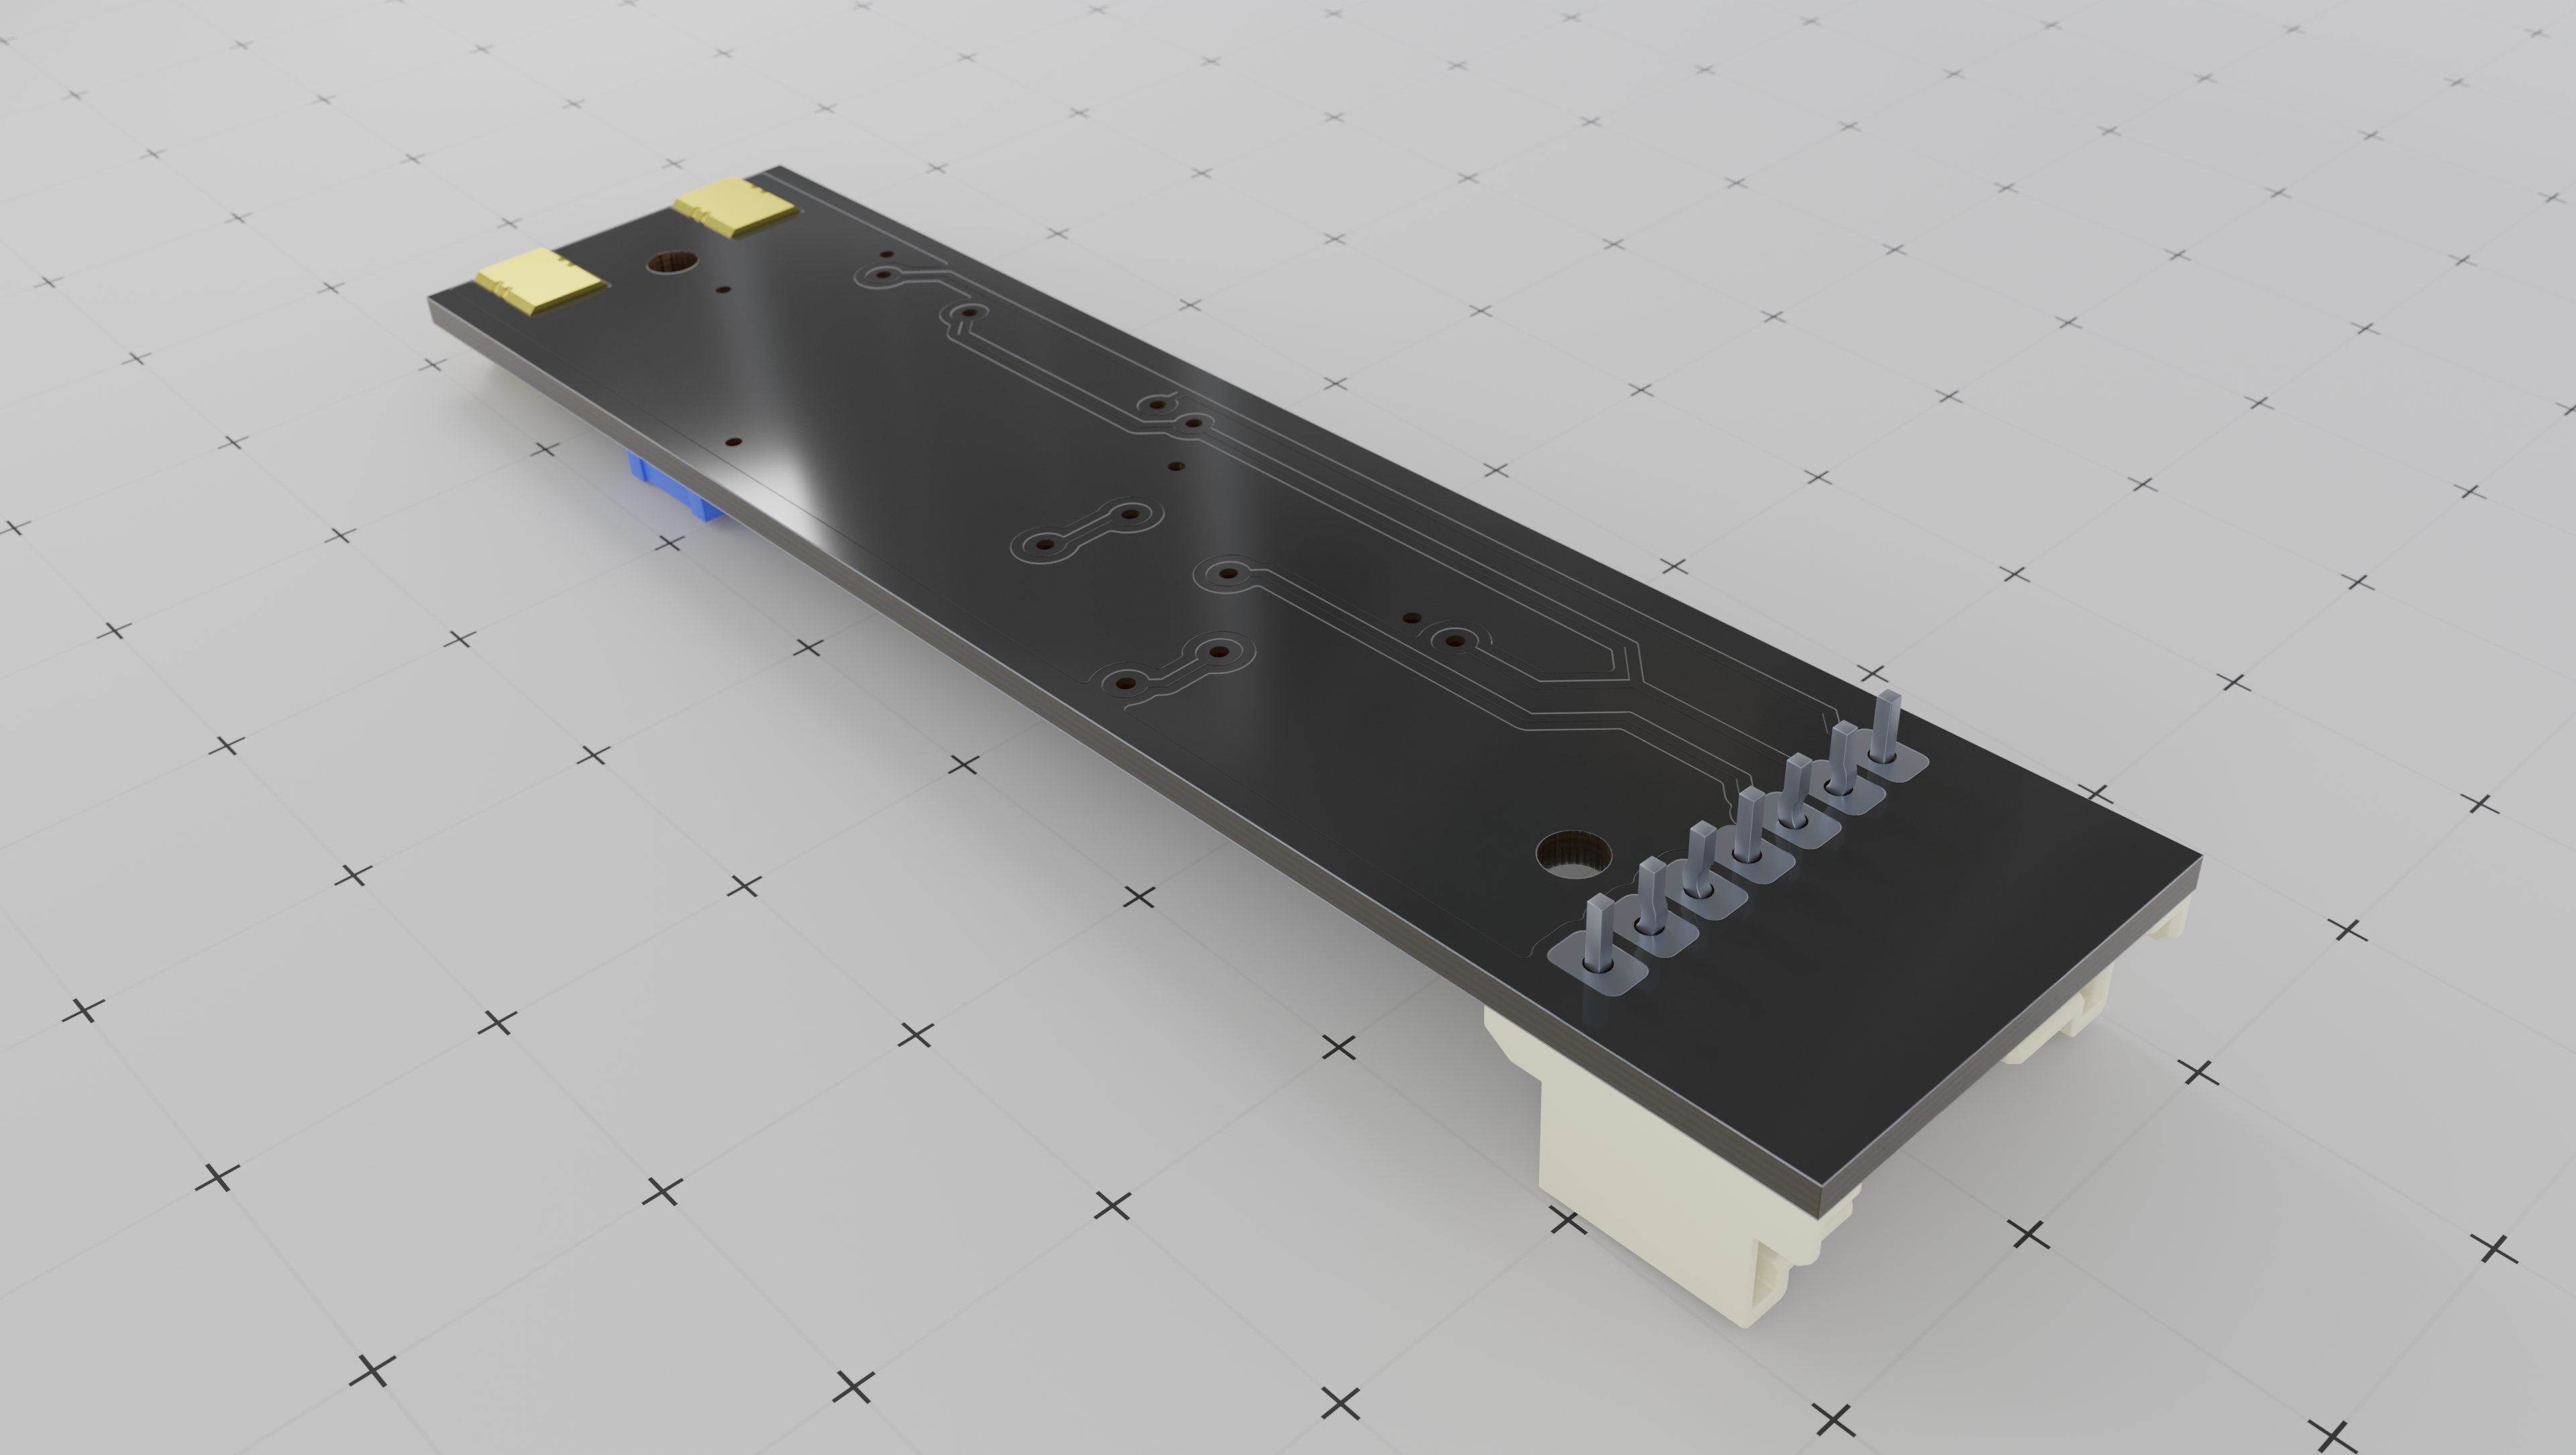
\includegraphics[width=\linewidth]{media/Render3.png}
                \end{minipage}
                \hspace{.04\linewidth}
                \begin{minipage}[H]{.45\linewidth}
                    \centering
                    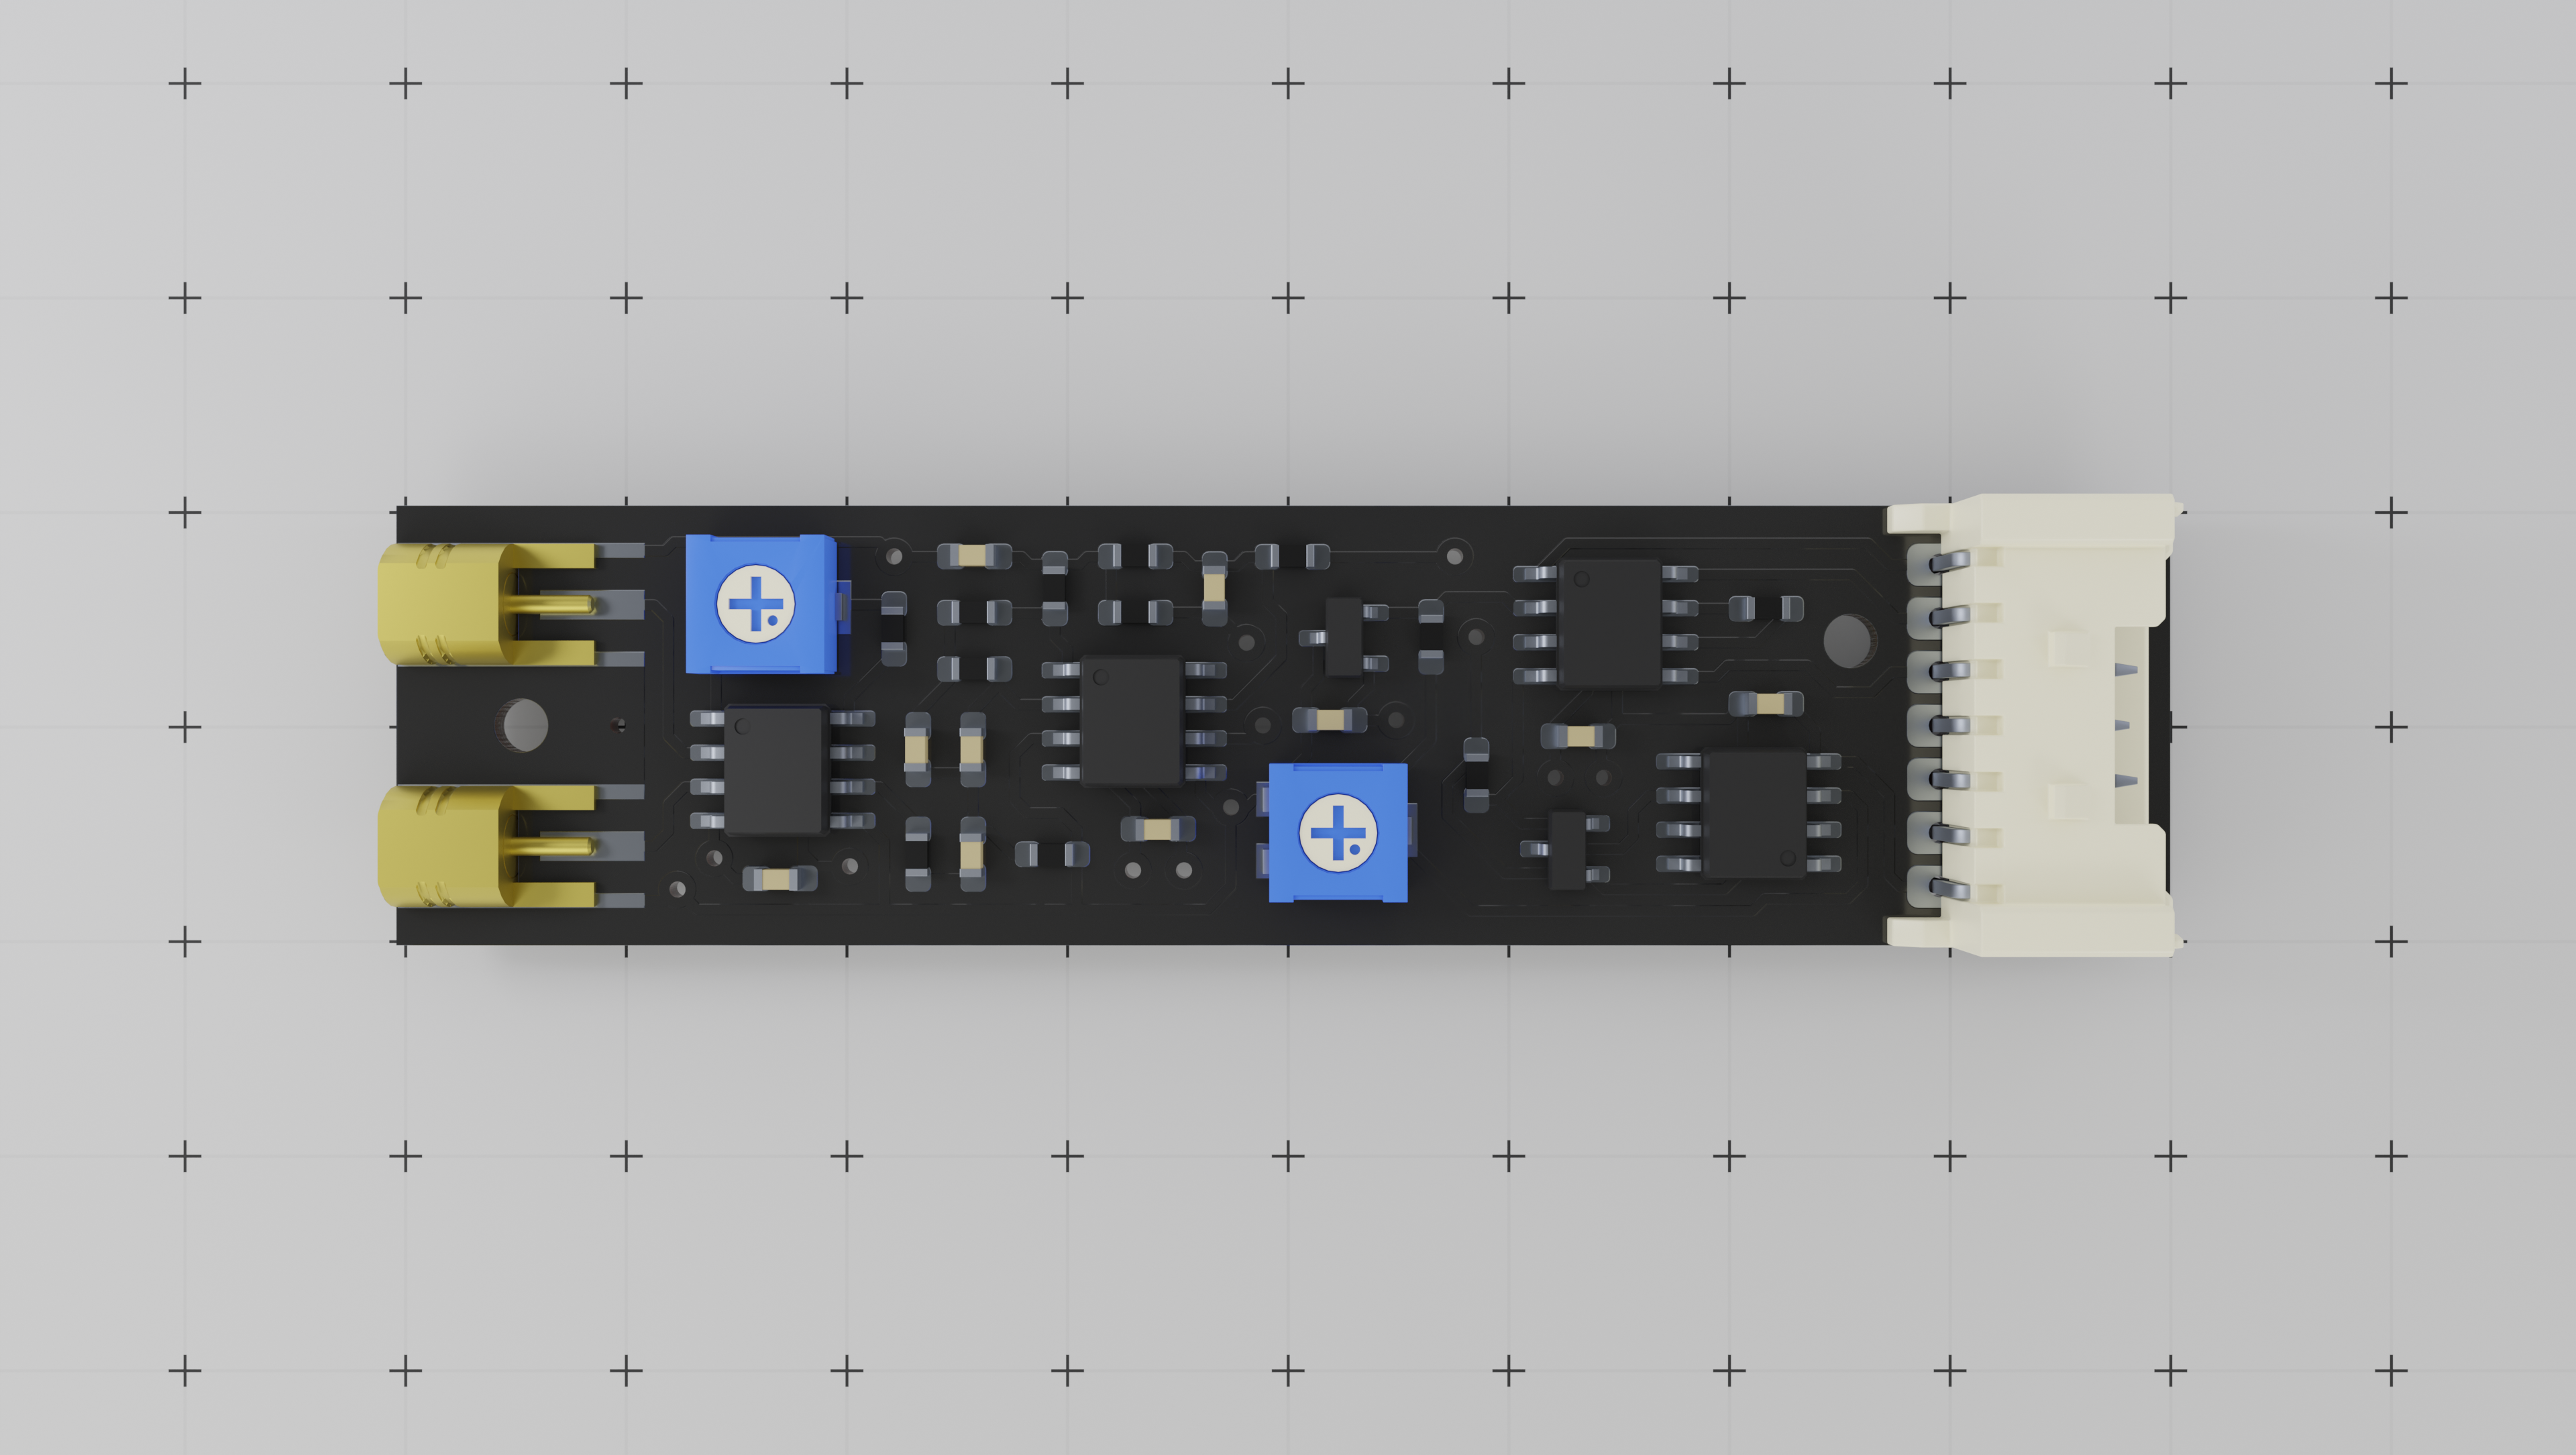
\includegraphics[width=\linewidth]{media/Render2.png}
                \end{minipage}
                \\
                \vspace*{.04\linewidth}
                \begin{minipage}[H]{.95\linewidth}
                    \centering
                    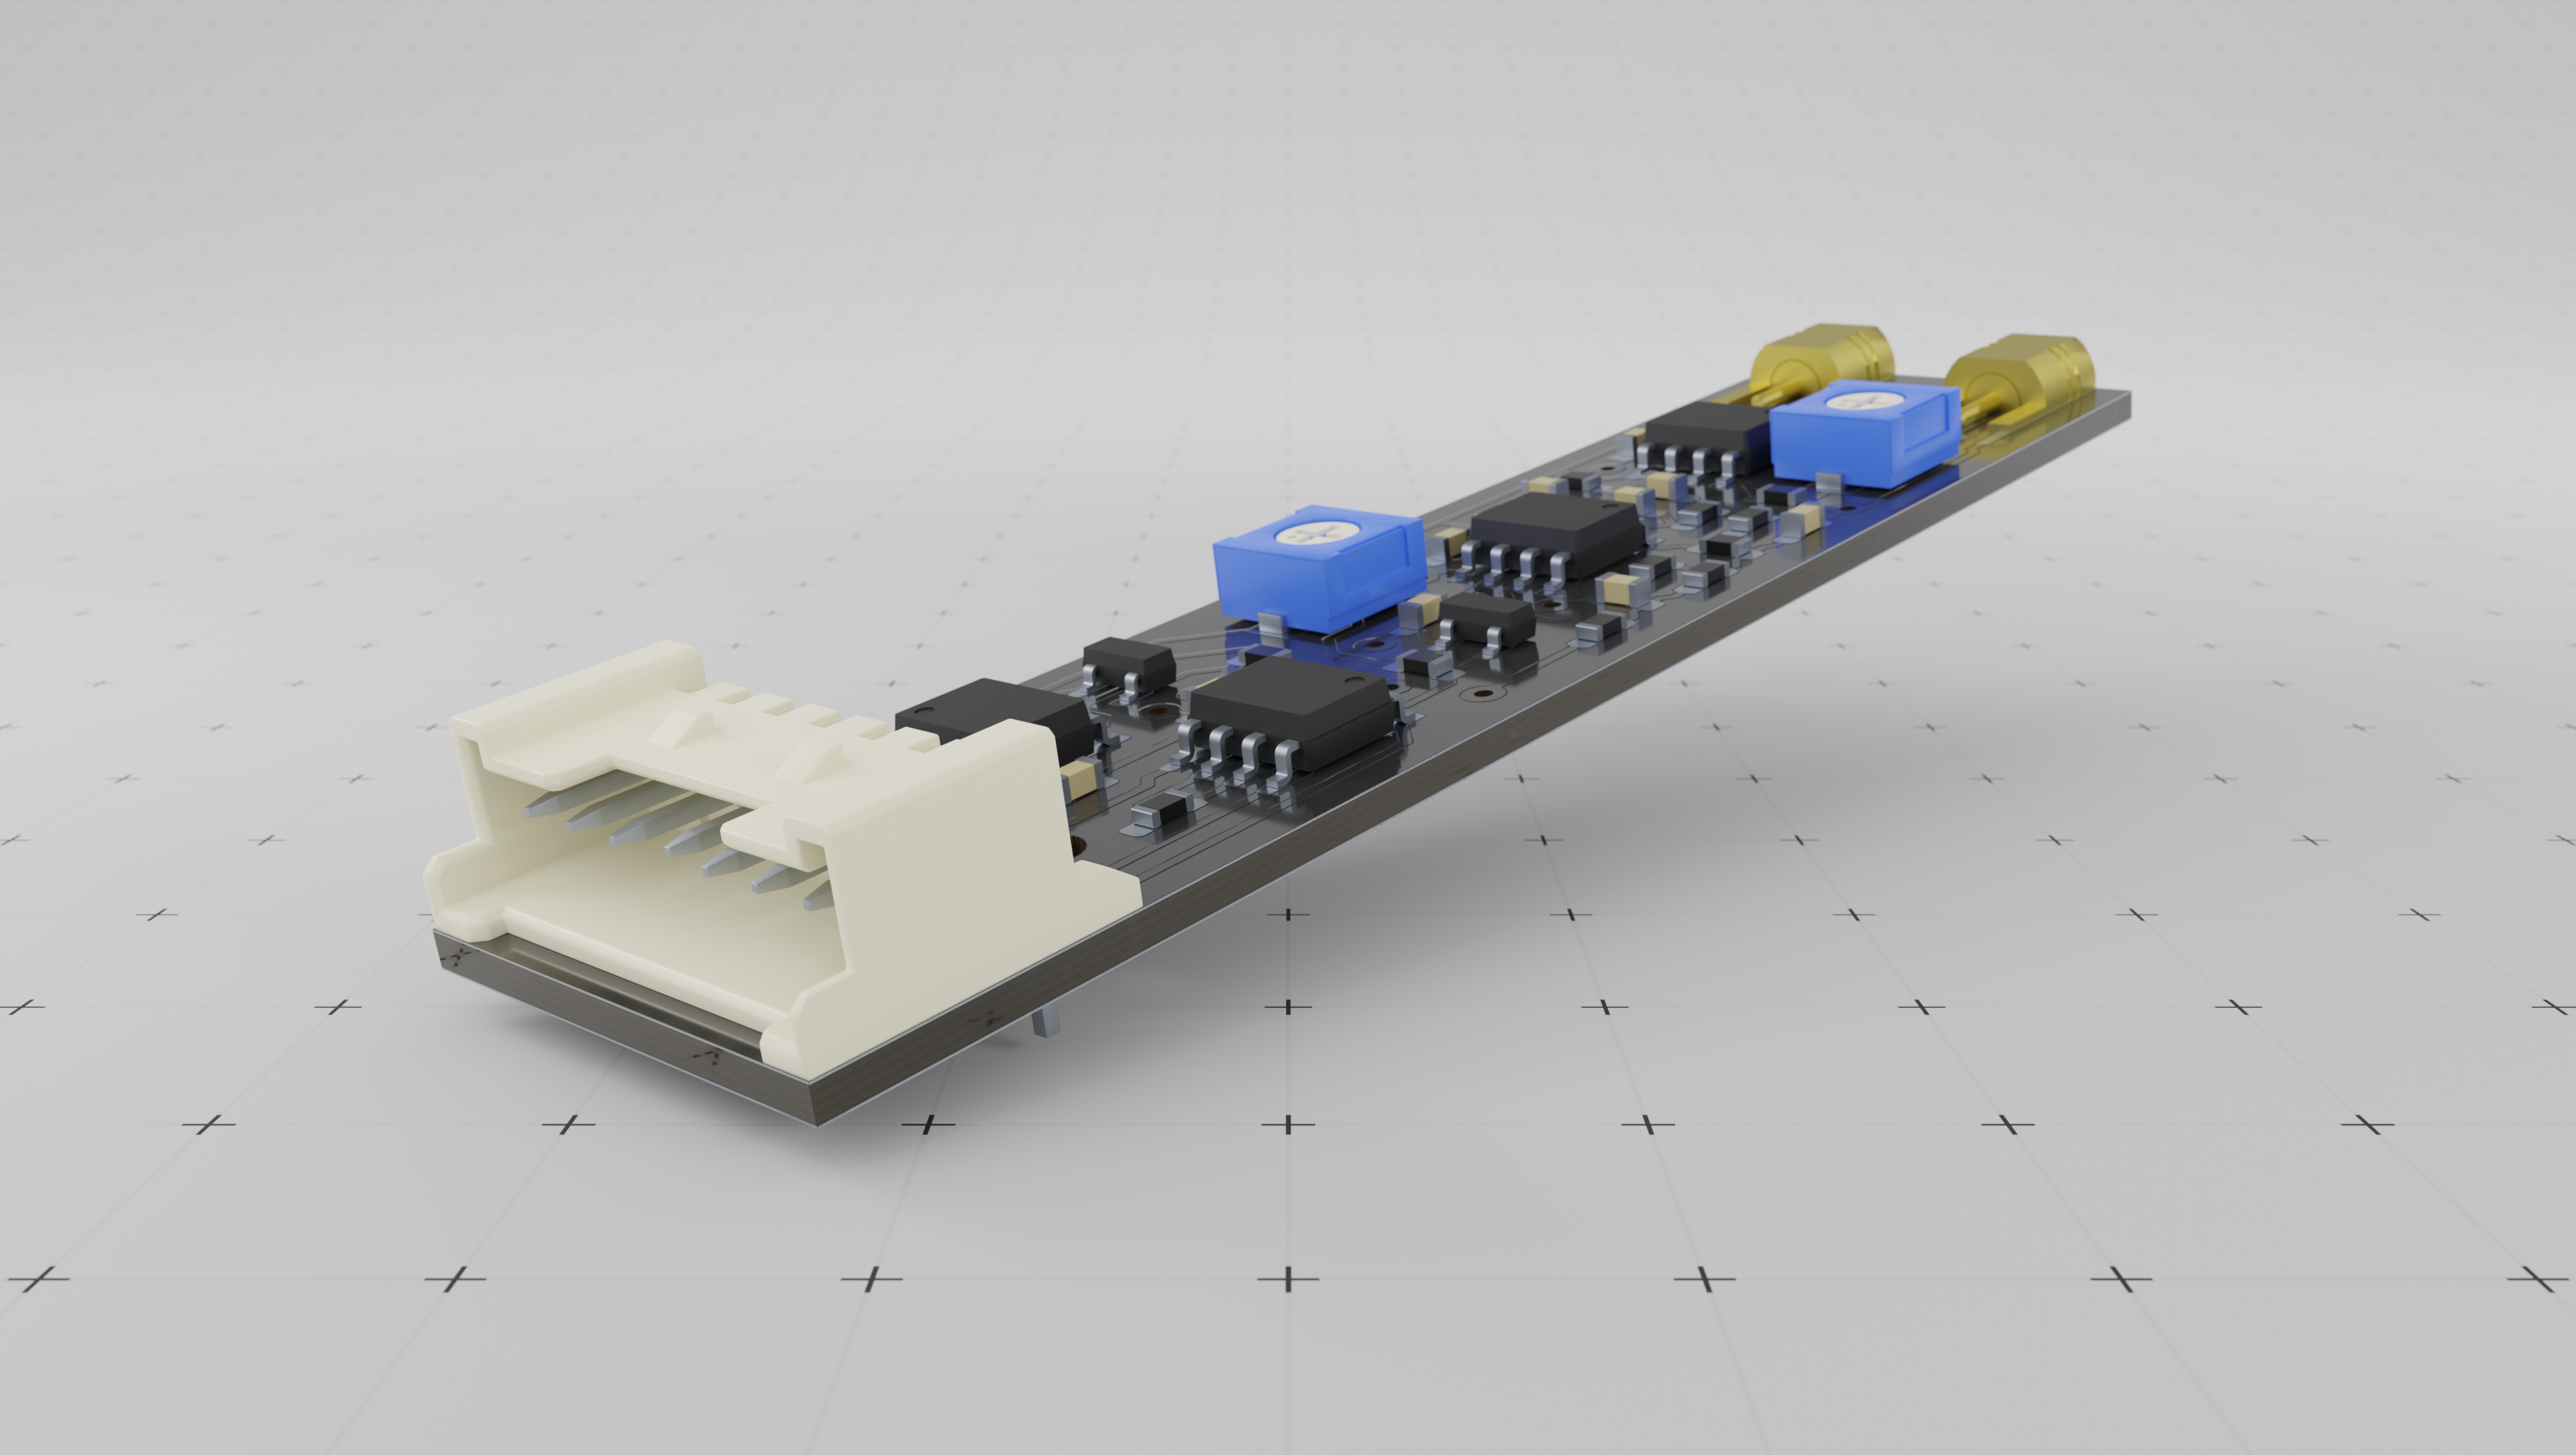
\includegraphics[width=\linewidth]{media/Render1.png}
                \end{minipage}
            \end{figure}
            
            \vspace*{\stretch{2}}
        \end{center}
    \end{titlepage}

    \clearpage
    % \listoftodos
    % \clearpage

    \section*{Abstract}
    \par I filtri analogici sono una componente inevitabile\footnote{Si discute dell'impossibilit\`{a} della loro eliminazione nella Sezione \ref{sec:ProjectDesignAbstractModel}, ultimo elenco di 6 punti}\todo{Controlla il numero di punti} ed indispensabile per la tecnologia del'XXI secolo: fanno parte delle componenti interiori dei dispositivi elettrici a partire dai smartphone e concludendo con apparechi scientifici di misurazione.
    Dalle sorgenti che si possono trovare in internet \`{e} molto complicato estrapolare le informazioni necessarie per essere in grado di fare un design pratico ed efficace dei filtri analogici.
    Proprio per questo motivo ci sono tanti individui tra le persone appassionate di elettrotecnica, le quali ritengono che il design dei filtri \`{e} facile da fare, ovvero con un paio di formule, che ovviamente danno delle informazioni, ma quello che lasciano fuori di considerazione viene coperto dal senso d'intuito della persona.
    Io, invece, ritengo che questo argomento deve essere perfettamente chiaro per tutte le persone che si reputano appassionate di elettrotecnica.
    Questo documento ha come argomento principale il design dei filtri analogici non solo a livello teorico, ma anche a livello pratico: alla fine del documento viene presentata una vera scheda che riesce a rilevare i segnali debolissimi dalla superficie della pelle, amplificarli e trasmetterli in forma di dati sul computer.
    La teoria che viene data \`{e} ampia, ma non troppo, proprio esatta per capire come funzionano i filtri, come si fa a fare dei design di quelli e in seguito realizzarli.
    \clearpage
    \tableofcontents

    \clearpage
    \section{Introduzione}\label{sec:Intro}
    \subsection{Motivazione}\label{sec:IntroMotivation}
    Prima dell'inizio dell'attivit\`{a} del lavoro di maturit\`{a} ho iniziato a notare sempre di pi\`{u} la mancanza di un mezzo di trasporto privato ed iniziai ad interessarmi della soluzione del problema.
    Tenendo conto del budget, della qualit\`{a} desiderata e delle specifiche caratteristiche: portatilit\`{a}, dimensioni e peso ridotto, riparabilit\`{a} e la possibilit\`{a} di sostituizione di un mezzo di trasporto, scelsi di creare uno skate elettrico.
    
    Una questione su cui mi soffermai maggiormente fu il telecomando perch\'{e} lo skate necessita il controllo della persona che lo conduce.
    Informandomi, scopersi che attualmente\footnote{Durante l'anno 2021} sul mercato tecnologico, gli skate elettrici possiedono telecomandi abbastanza semplici, dotati di pulsanti assieme a qualche sua variazione di tipo analogico\footnote{Con pi\`{u} di due stati} per poter dosare la potenza con cui attivare i motori.
    Dunque, decisi\footnote{I fattori che hanno avuto influenza sulla scelta saranno spiegati nella Sezione \ref{sec:IntroReader}} di aderire ad un'idea molto meno standard che, inoltre, mi risulta o nuova o raramente utilizzata: concetto del controllo gestuale in combinazione con un mezzo di trasporto.
    
    Per una coincidenza comoda di date, durante lo sviluppo del progetto ebbi anche la necessit\`{a} di fare un lavoro di maturit\`{a} con un'argomento su robotica, ovvero anche fisico-matematica, che implicava la creazione di un prototipo robotico in base a degli studii e a delle ricerche personali. Ovviamente, cercai di mantenere il progetto in corso, che purtroppo, se preso intero, fu eccessivamnete ampio per un lavoro di maturit\`{a}. Allora guidato dalla positivit\`{a} di creare un dispositivo che non occuperebbe la mano durante l'uso\footnote{Durante la caduta o qualsiasi situazione imprevista \`{e} desiderata l'immediata disponibilit\`{a} delle mani e inoltre ritengo che aumenti la comodit\`{a}} e dalla propria opinione dell'originalit\`{a} dell'idea, decisi di portare una sua piccola parte: la parte analogica del sensore elettromiografico\footnote{I termini e le motivazioni della scelta verranno chiariti nella Sezione \ref{sec:IntroReader}}, in seguito\footnote{Sezione \ref{sec:IntroMotivation}} verr\`{a} chiarito che principalmente si tratta di un filtro.
    
    \subsection{Obiettivo del lavoro}\label{sec:IntroAim}
    \noindent L'obiettivo di questo lavoro di maturit\`{a} \`{e}:
    \begin{enumerate}[label=\emph{(\roman*)}]
        \item Introdurre il lettore al concetto dei filtri e del loro funzionamento in termini dei segnali
        \item Fornire la terminologia loro riguardante
        \item Rispondere a domande che sono sorte durante lo sviluppo del progetto
        \item Portare a conoscenza di considerazioni da prendere durante design teorici e pratici 
        \item Costruire un prototipo come verifica del concetto
    \end{enumerate}
    Inoltre, tante conoscenze che verranno date nel lavoro di maturit\`{a} sono applicabili in diversi altri campi, ad esempio: il modello matematico dei filtri \`{e} completamente valido anche per i filtri digitali e i dettagli pratici\footnote{Come nella Sezione \ref{sec:BuildingHardware}} \todo{aggiungi parte dei condensatori bypass, induttanza, ground plane e skin effect} sul design dei circuiti sono applicabili a quasi ogni altra tipologia di circuito di precisione.
    
    Il contenuto include anche il procedimento mentale\footnote{Un ragionamento dettagliato sui motivi che guidano all'uso di un filtro, e le conseguenze che implica il loro utilizzo} precedente il processo dello sviluppo del filtro, che aiuta ad integrare il filtro in un progetto, al posto di separare il concetto e lasciare delle domande cruciali senza risposte, che possono sorgere durante il lavoro su un prossimo progetto.
    
    \subsection{Organizzazione del lavoro}\label{sec:IntroOrganization}
    Le caratteristiche specifiche del progetto, come le metodiche di project management\footnote{Il termine e la caratteristica che indica saranno discusse nella Sezione \ref{sec:ProjectCharacteristics}} utilizzate e la dimensione del progetto a confronto con la sua parte portata al lavoro di maturit\`{a}, stanno a dettare delle regole di organizzazione del progetto che discuto nella presente Sezione.
    Se il procedimento dato dalle metodiche e dalla complessit\`{a} del progetto, venisse documentato in modo cronologico, il contenuto risulterebbe essere troppo ampio nello scritto, poco coerente al tema del lavoro di maturi\`{a} e frequentemente confusionale.
    
    \begin{samepage}
        \noindent Lo schema che seguo durante la documentazione di tutto il lavoro di maturit\`{a} per risolvere i problemi di organizzazione \`{e} lo seguente:
        \begin{enumerate}[label=\emph{(\roman*)}]
            \item Teoria \& Pratica
            \item Caratteristiche
            \item Design
        \end{enumerate}
    \end{samepage}
    Conviene notare che questo schema tripartito non cerca di dare forma a tutto il lavoro di maturit\`{a} in stile "\emph{Introduzione}", "\emph{Corpo del lavoro}", "\emph{Conclusioni}", ma tenta riordinare i contenuti in gruppi concettuali per poi costruirci sopra un discorso coeso, con un andamento costante e logico, nel frattempo non negando la presenza dello schema principale come il "de facto"\footnote{Preso come standard formale per l'ovviet\`{a} a gran numero di persone} standard appena citato.
    
    La parte della \emph{Teoria \& Pratica} serve a fornire le informazioni necessarie al lettore per concepire gli agromenti toccati nelle parti seguenti.
    La parte delle \emph{Caratteristiche} serve a capire che caratteristiche deve possedere o possiede il soggetto, quali di quelle sono ad influire la prossima parte e i seguenti soggetti gerarchialmente sottostanti.
    La parte del \emph{Design} \`{e} la parte dove si motivano e si affermano, attraverso dei ragionamenti, delle scelte che si sono fatte, che sono sempre strettamente collegate alle parti precedenti del medesimo soggetto e dei soggetti precedenti.
    Ovviamente, le parti delle \emph{Caratteristiche} e del \emph{Design} contengono delle parti teoriche e pratiche, ma quando le informazioni prese in considerazione diventano troppo ampie nel descriverle in una Sezione, si ragruppano in un'altra Sezione di \emph{Teoria \& Pratica} che viene messa a precedere le due.
    
    \begin{samepage}
        \noindent L'esempio potrebbe essere:
        \begin{enumerate}[label=\emph{(\roman*)}]
            \item Sezione \ref{sec:IntroFiltersSignals} $\Rightarrow$ \emph{Teoria \& Pratica}
            \item Sezione \ref{sec:ProjectCharacteristics} $\Rightarrow$ \emph{Caratteristiche}
            \item Sezione \ref{sec:ProjectDesign} $\Rightarrow$ \emph{Design}
        \end{enumerate}
    \end{samepage}

    \subsection{Introduzione al lavoro}\label{sec:IntroReader}
    Per introdurre il lettore al lavoro di maturit\`{a} in questa Sezione spiego dei concetti di base, per essere in grado di seguire il discorso e riporto il ragionamento in forma sintetizzata, che appartiene alla parte del lavoro svolto prima di arrivare alla tappa dello sviluppo dei sensori.

    Tra la teoria e tra la pratica, io preferisco iniziare dalla parte teorica per mostrare al lettore un modello semplice che pu\`{o} essere sviluppato, complicato e perfezionato nel corso della lettura.
    
    Generalizzando massimamente, il problema che si cerca di risolvere \`{e} la trasmissione di informazioni ad una piccola distanza.
    Ho ritenuto, che l'unica scelta logica attraverso la quale cercare la soluzione, sarebbe l'elettronica per le possibilit\`{a} di creare dispositivi di dimensioni compatte e di trasmettere informazioni attraverso RF\footnote{Frequenze radio} che sono per definizione una caratteristica del fenomeno dell'elettromagnetismo\footcite["Il campo" (elettromagnetico) "pu\`{o} essere visto come la combinazione di un campo elettrico e un campo magnetico"]{Electromagnetism:Wiki} \footcite["L'elettricità è correlata al magnetismo, essendo entrambi parte del fenomeno dell'elettromagnetismo"]{Electricity:Wiki}.
    In seguito ho applicato una tecnica di astrazione con l'aiuto del paragone ai \emph{Input/Output} \footcite[]{IO:Wiki}.
    Consiste nel capire di quali "\emph{Output}\footnote{Uscite di informazioni}" possibili \`{e} dotato il soggetto dal quale si dovrebbero raccogliere le informazioni, che cosa coloro causerebbero dal punto di vista fisico e infine scegliere dei fenomeni per prossimamente convertirli in un feedback\footnote{Richiamo}, nel nostro caso un feedback elettrico.
    Nel caso dell'uomo come soggetto, solo il \emph{movimento} della persona o delle sue parti del corpo e la produzione dei \emph{suoni} \footnote{Voce, battito di mani, fischio, ecc...} possono permettere l'espressione delle informazioni.
    Ho scelto la trasmissione di informazioni attraverso i movimenti proprio per non influire sui suoni, per evitare possibili interferenze\footnote{Sono possibili anche con i movimenti, ma oggettivamente sono pi\`{u} rare mettendo come motivo la possibilit\`{a} dei suoni di diffondersi nell'aria} e per la piccola necessit\`{a} di avere un vocabolario eccessivamente complesso\footnote{Detto a riguardo del controllo vocale}.
    I movimenti possono essere di qualsiasi aspetto, come portare il peso del corpo avanti o indietro rispetto al mezzo, che per\`{o} si manifest\`{o} senza abbastanza granularit\`{a} di controllo e ad interferire con l'utilizzo del mezzo\footnote{Si deve avere un ideale senso di equilibrio per mantenere controllo durante momenti come accelerazione e frenata}.
    \clearpage  
    \noindent Siccome nessun altro movimento sembrava abbastanza comodo, l'ultima possibilit\`{a} rimantente fu quella della mano, che dimostr\`{o} essere molto efficace per la sua granularita di controllo e flessibilit\`{a}.
    Applicando una seconda volta la tecnica appena riferita\footnote{Tecnica utilizzata col paragone ai Input/Output},
    ci furono differenti idee di variazioni possibili dell'"\emph{Output}" del soggetto\footnote{Analisi Input/Output della mano} \emph{(indicato coi numeri)} ed idee di soluzioni per usufruirne \emph{(indicato con le lettere)}:
    \begin{enumerate}[label=\emph{(\arabic*)}]
        \item Cambiamento della posizione delle dita e della mano
            \begin{enumerate}[label=\emph{(\alph*)}]
                \item Guanto con rotary encoder\footnote{Encoder roatativo} \footnote{Ci sono diversi tipi di rotary encoder: a contatto, a luce, a effetto di Hall (a calamita)}\emph{(Figura \ref{fig:IdeaEncoderGlove})} con molla e fili, oppure flex sensors\footnote{Sensori di flessione} \footnote{Cambiano la loro resistenza in base a quanto sono piegati}\emph{(Figura \ref{fig:IdeaFlexGlove})}
                \item Bracciale con un radar elettromagnetico come il chip "Soli"\footcite[]{GoogleATAP:Wiki} \emph{(Figura \ref{fig:IdeaRadarGlove})}
                \item Sensori MEMS\footnote{Combinazione di giroscopio, accelerometro e alcune volte sensori del campo magnetico terrestre per identificare precisamente la posizione nello spazio} su ogni dito e sulla mano \emph{(Figura \ref{fig:IdeaMEMSGlove})}
            \end{enumerate}
        \item Cambiamento del diametro dei muscoli per la contrazione
        \item Cambiamento del campo elettrico nel nervo per il segnale che porta, di conseguenza anche nel muscolo per la sua contrazione \label{ItemDeltaChoice}
            \begin{enumerate}[label=\emph{(\alph*)}]
                \item Elettrodi ad ago \emph{(Figura \ref{fig:IdeaNeedleEMGBand})}, a contatto superficiale o a capacit\`{a} superficiale \emph{(Figura \ref{fig:IdeaSurfaceEMGBand})} che sono soggetti al cambiano di carica elettrica per i campi elettromagnetici generati dal muscolo e/o dal nervo \label{ItemEMG}
            \end{enumerate}
    \end{enumerate}

    \begin{figure}[H]
        \centering
        \begin{minipage}[H]{.32\linewidth}
            \centering
            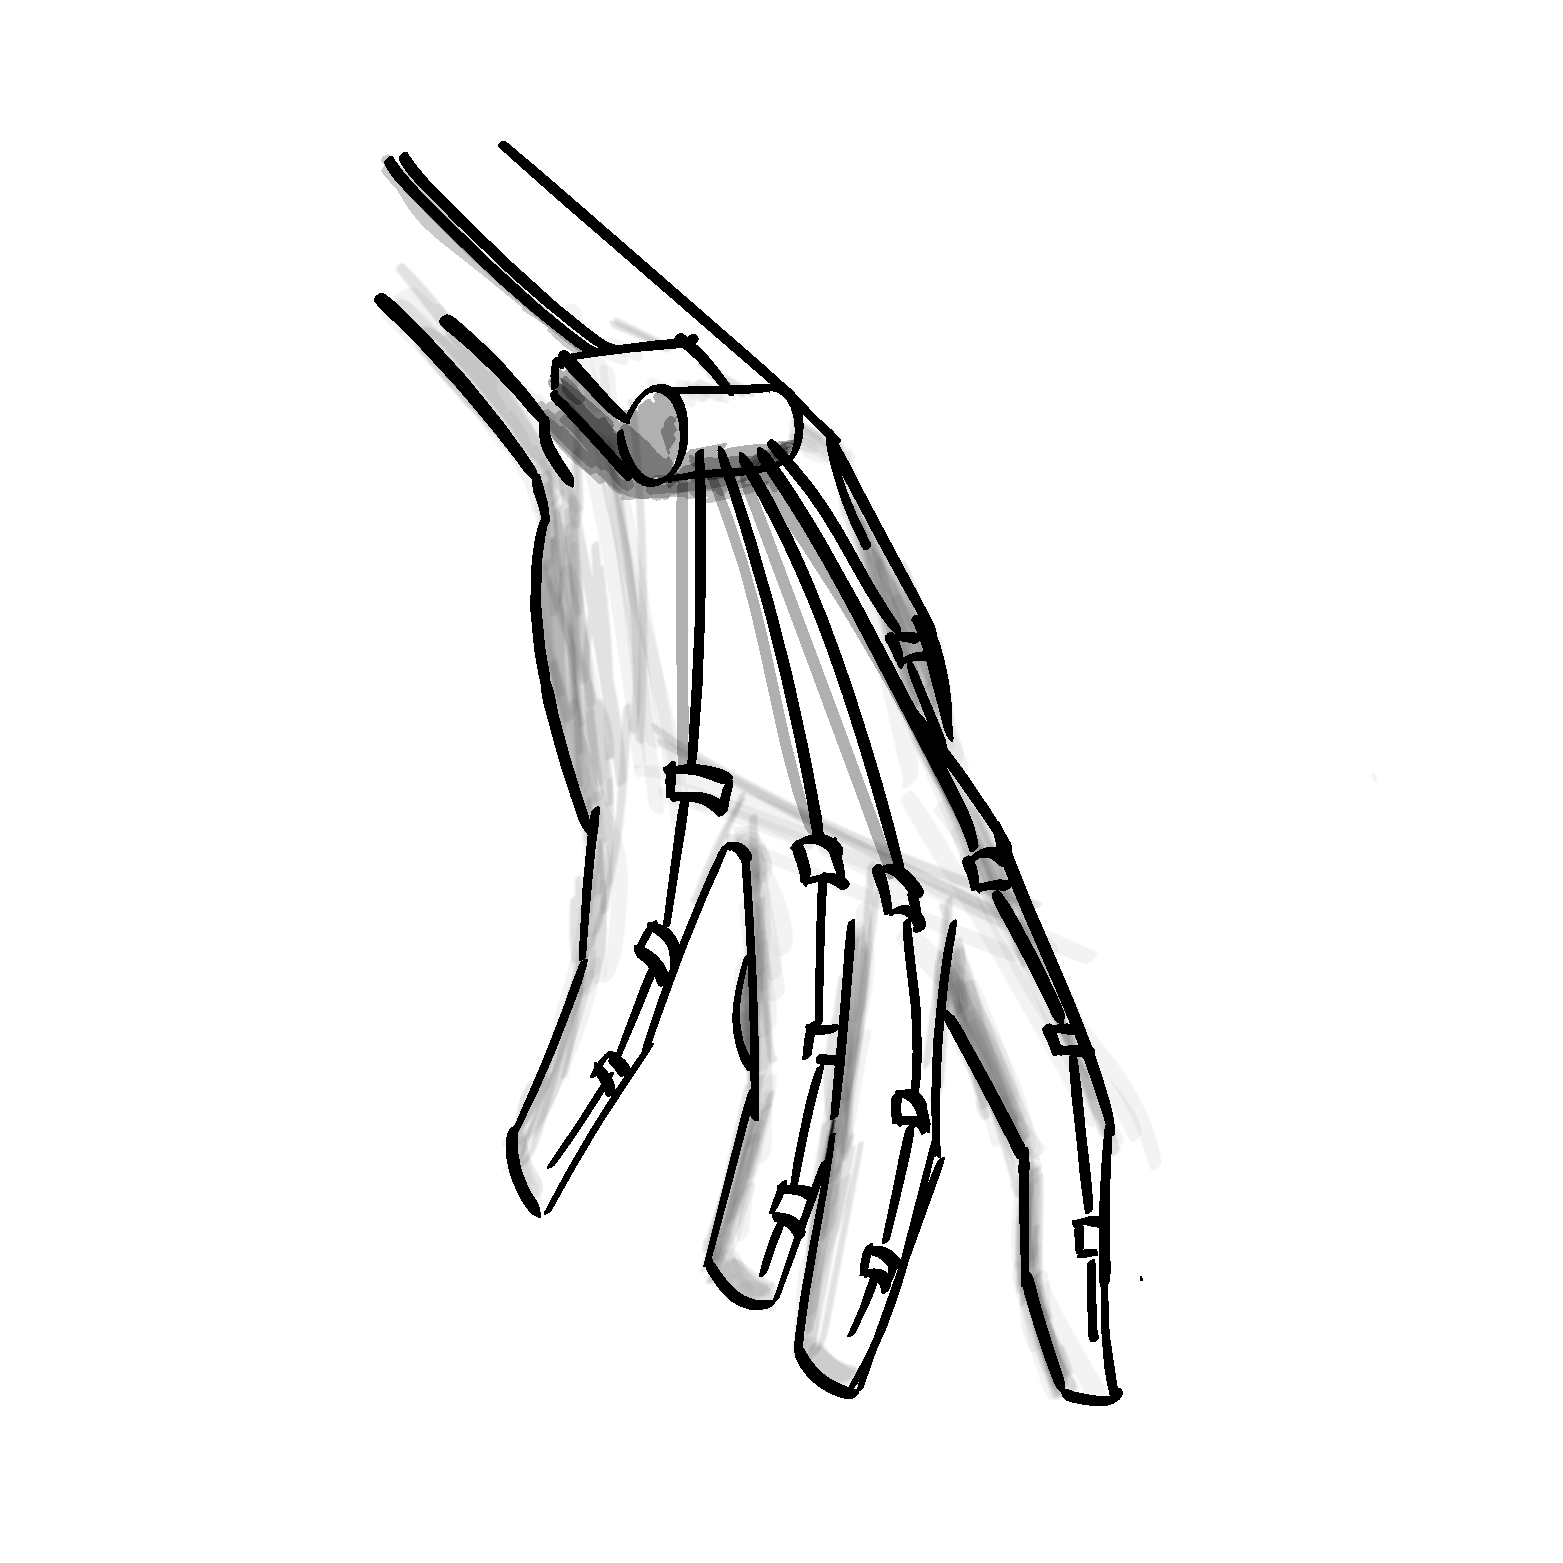
\includegraphics[page=1, width=\linewidth]{media/Ideasheet1.pdf}
            \subcaption{}\label{fig:IdeaEncoderGlove}
        \end{minipage}
        \begin{minipage}[H]{.32\linewidth}
            \centering
            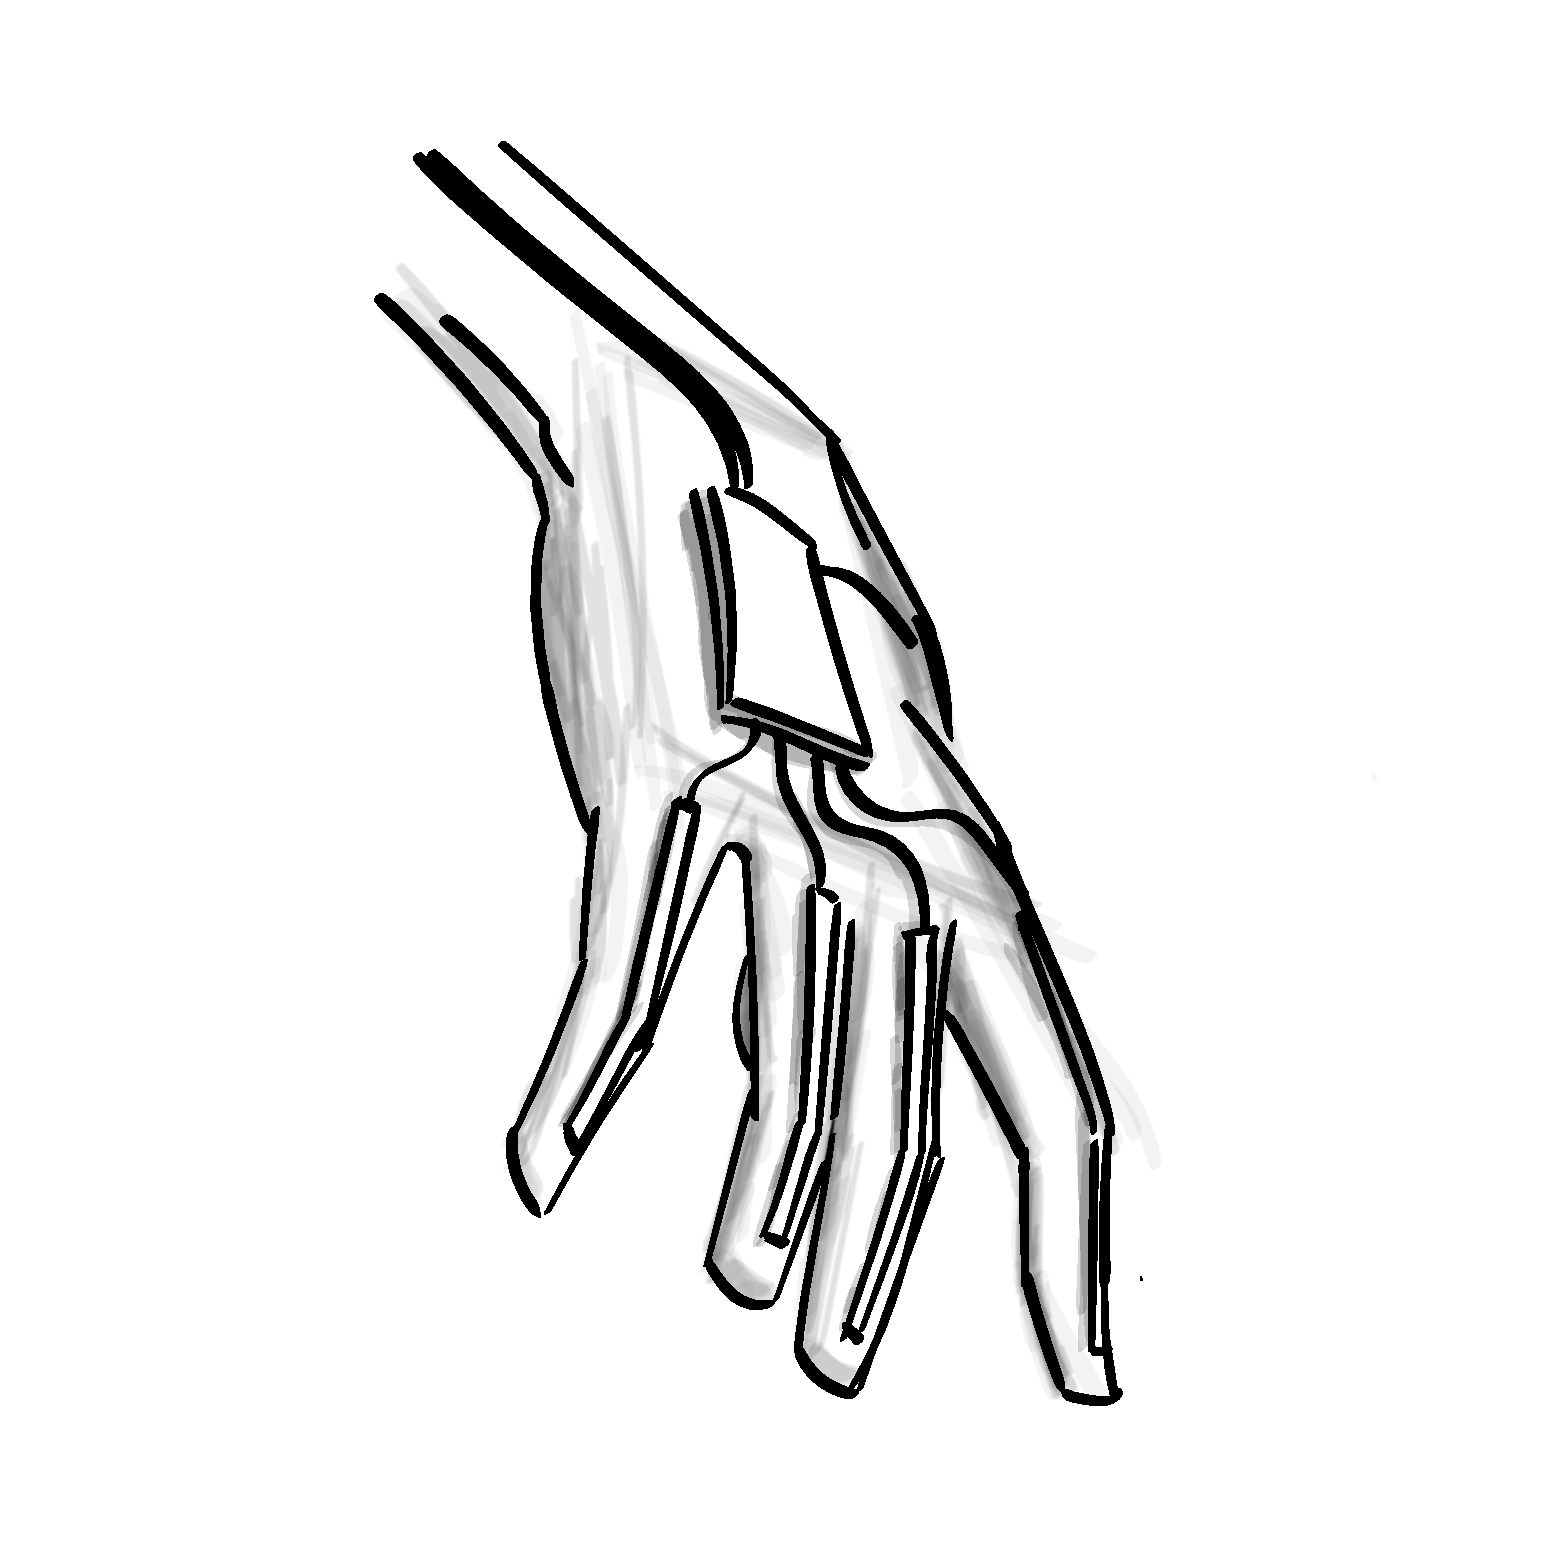
\includegraphics[page=1, width=\linewidth]{media/Ideasheet2.pdf}
            \subcaption{}\label{fig:IdeaFlexGlove}
        \end{minipage}
        \begin{minipage}[H]{.32\linewidth}
            \centering
            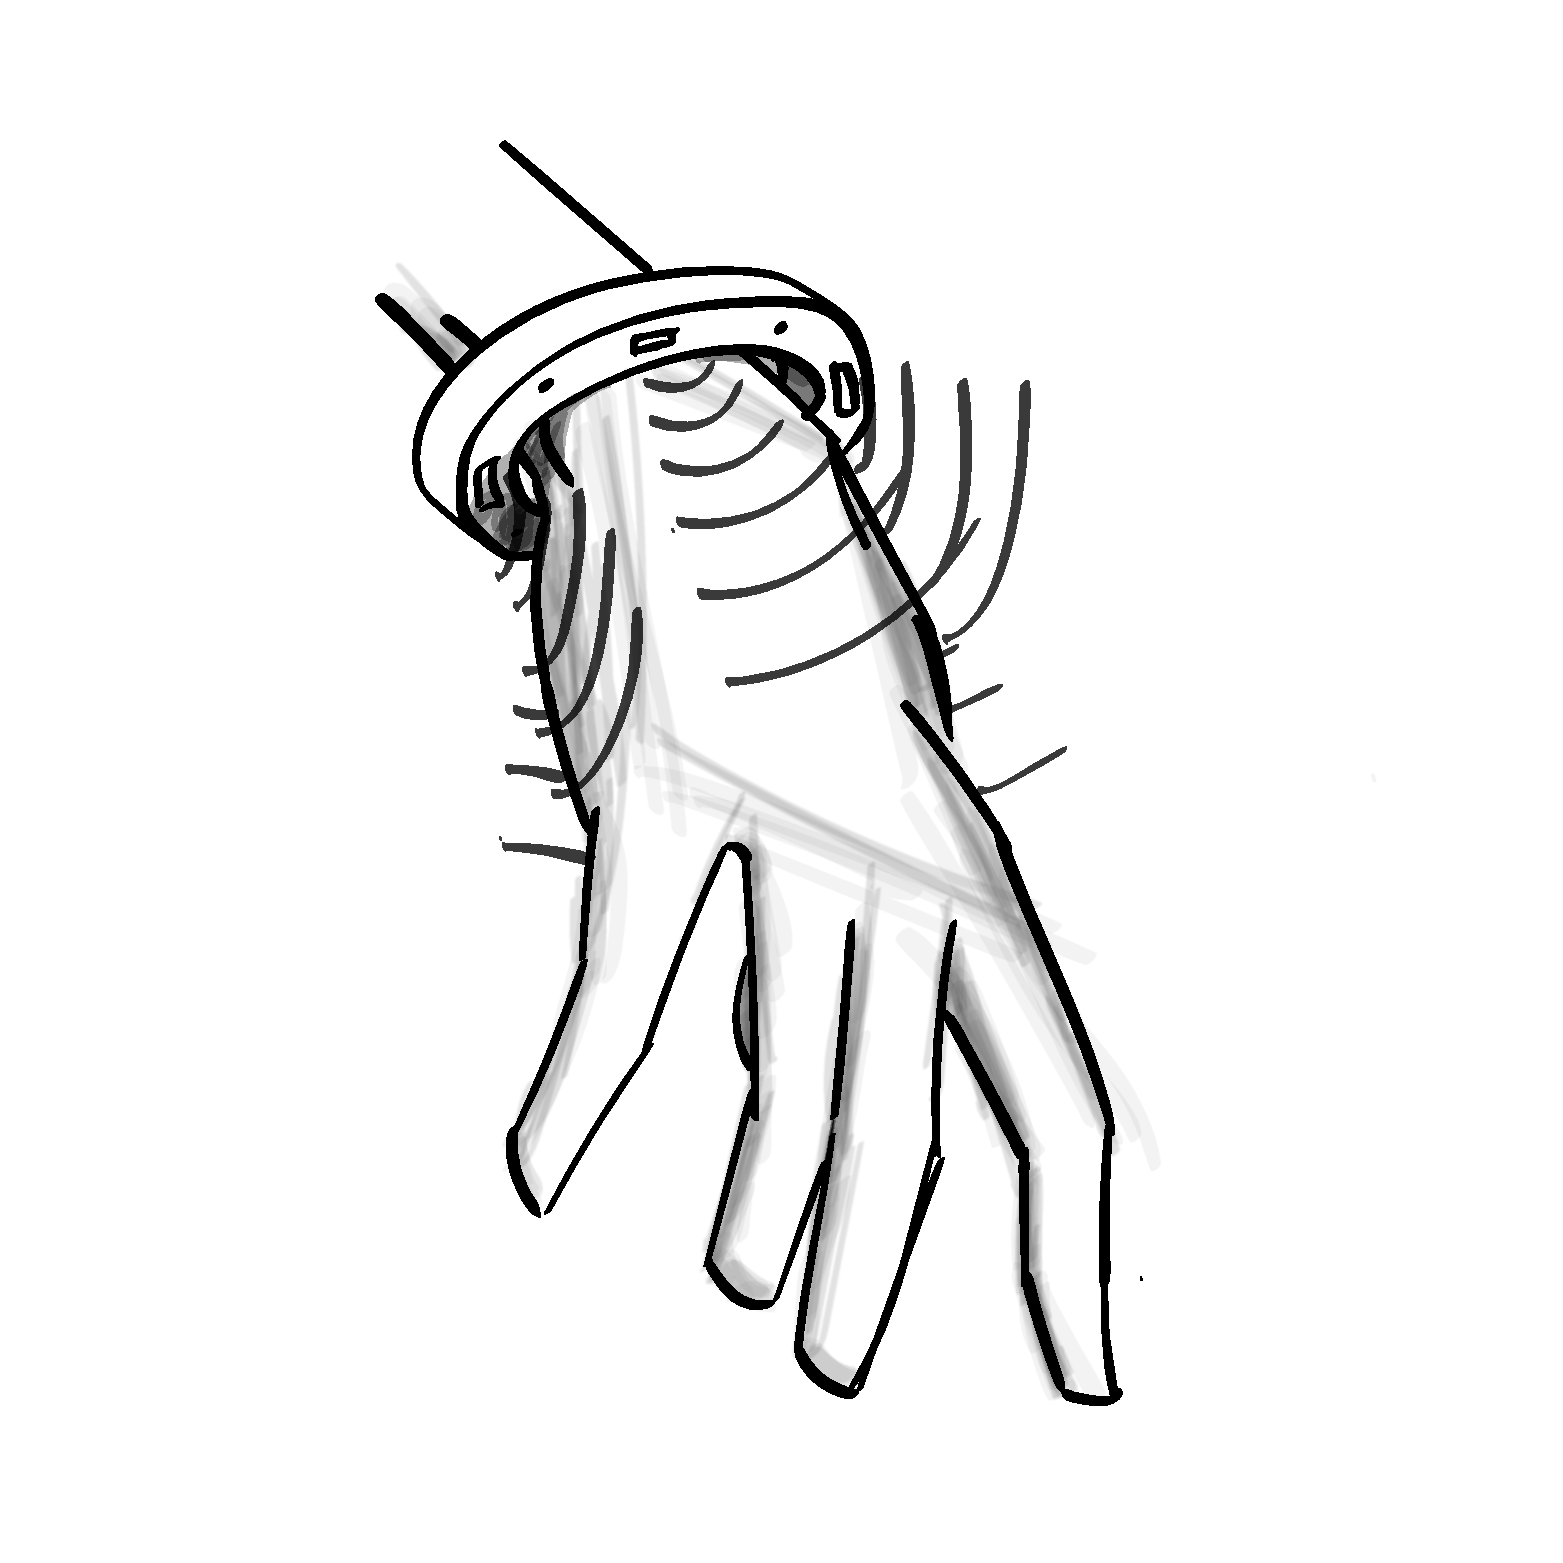
\includegraphics[page=1, width=\linewidth]{media/Ideasheet3.pdf}
            \subcaption{}\label{fig:IdeaRadarGlove}
        \end{minipage}
        \begin{minipage}[H]{.32\linewidth}
            \centering
            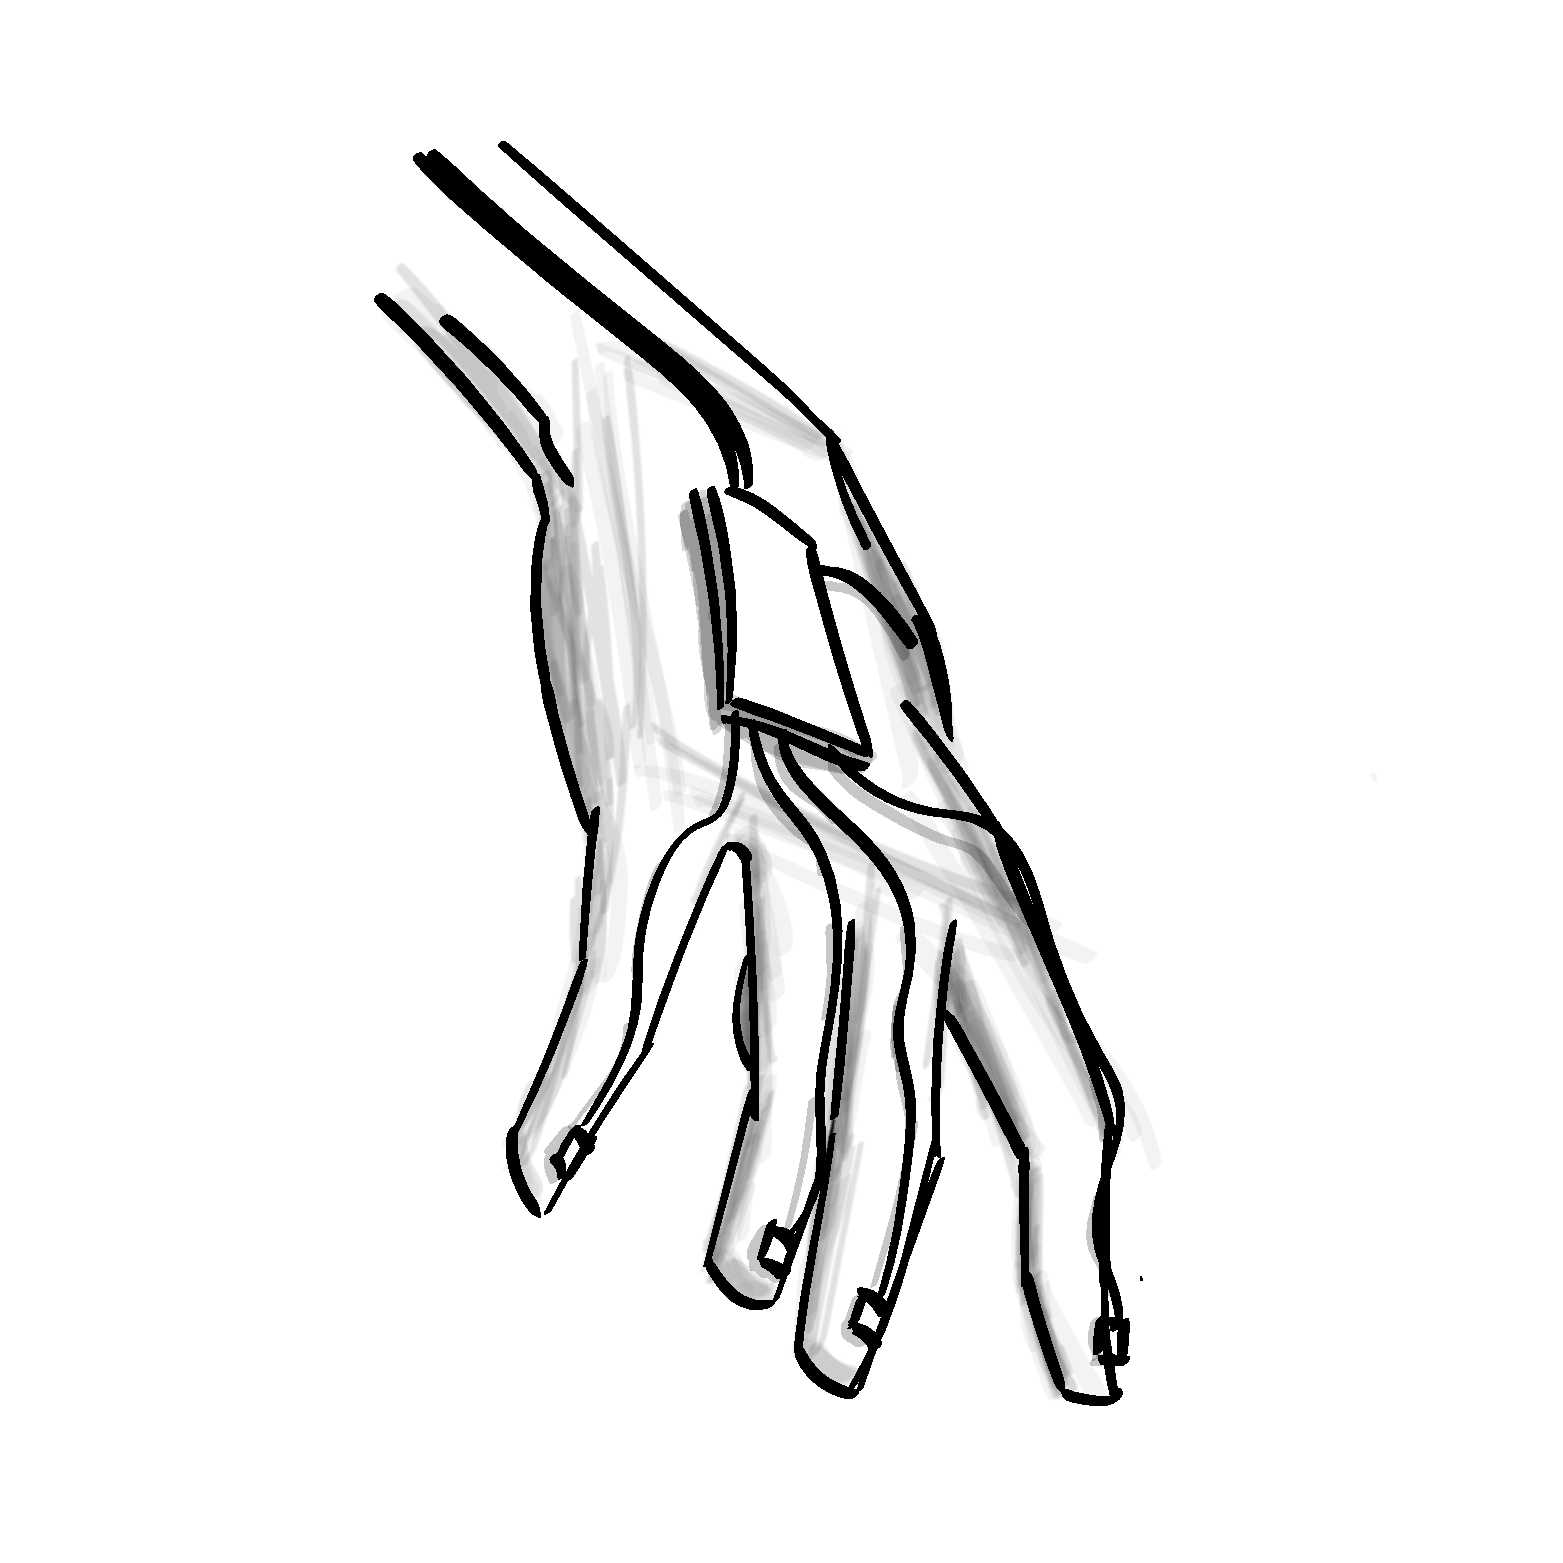
\includegraphics[page=1, width=\linewidth]{media/Ideasheet4.pdf}
            \subcaption{}\label{fig:IdeaMEMSGlove}
        \end{minipage}
        \begin{minipage}[H]{.32\linewidth}
            \centering
            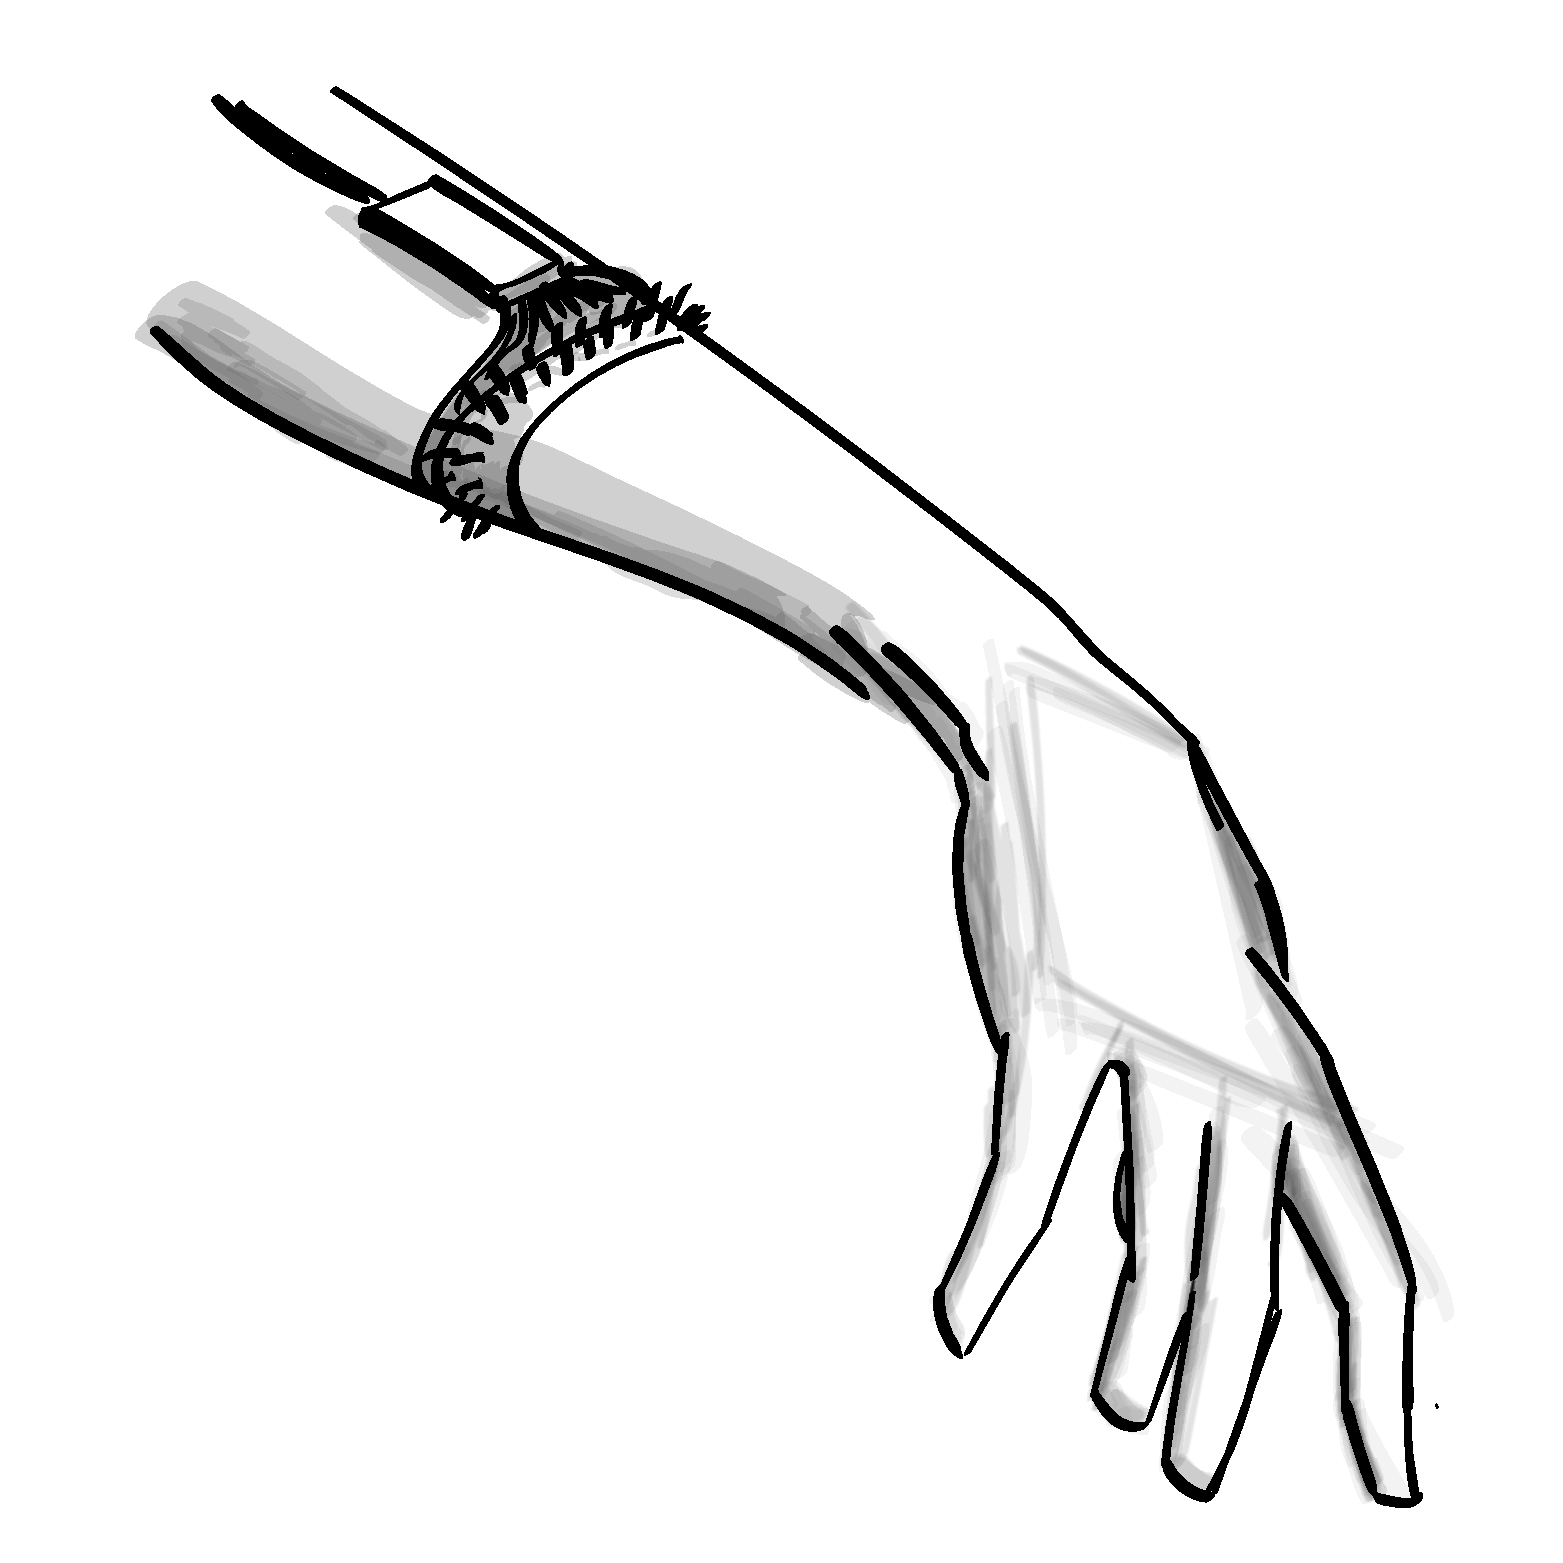
\includegraphics[page=1, width=\linewidth]{media/Ideasheet5.pdf}
            \subcaption{}\label{fig:IdeaNeedleEMGBand}
        \end{minipage}
        \begin{minipage}[H]{.32\linewidth}
            \centering
            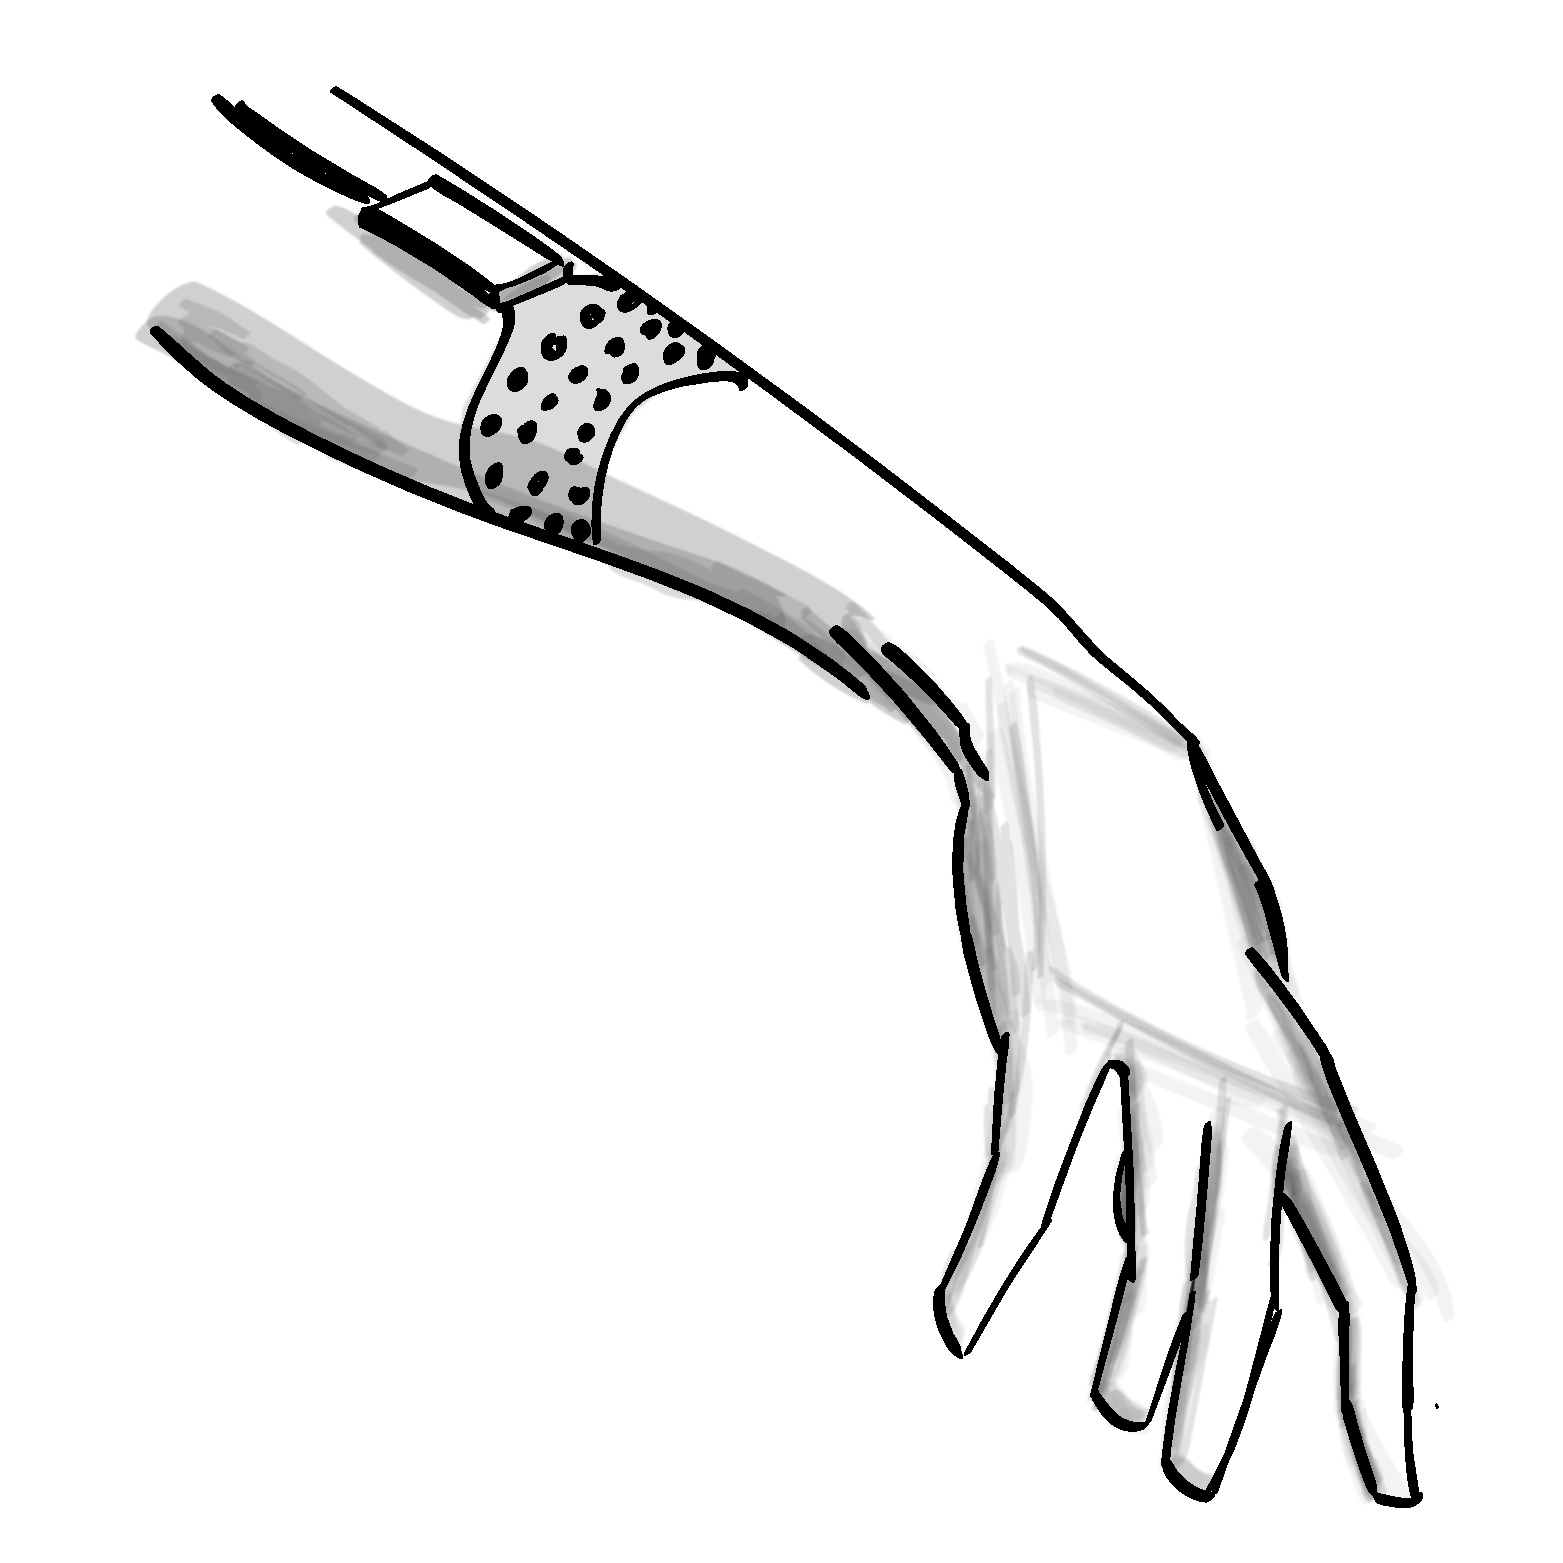
\includegraphics[page=1, width=\linewidth]{media/Ideasheet6.pdf}
            \subcaption{}\label{fig:IdeaSurfaceEMGBand}
        \end{minipage}
        \caption{Idee}\label{fig:Idea}
    \end{figure}
    
    Come si pu\`{o} capire dalla Sezione \emph{\ref{sec:IntroMotivation}}, ho scelto l'idea \ref{ItemDeltaChoice}\ref{ItemEMG} e di quella ovviamente la variazione dei metodi meno invasiva possibile, come la \emph{sEMG} \footnote{Surface Electromyography, ovvero elettromiografia superficiale} per le condizioni d'uso che possono essere classificate di grado automotivo\footcite[]{AutomotiveGrade:Wiki}\footnote{Si intende il grado di affidabilit\`{a} dei componenti dato dalle loro caratteristiche come resistenza a temperature elevate, a vibrazioni e ad altri impatti fisici} e perfino estreme.
    I lati negativi della scelta sono la debolezza del segnale iniziale a confronto con le \emph{EMI} \footcite[Interferenza elettromagnetica]{EMI:Wiki} dell'ambiente, ma questo problema \`{e} facilmente risolvibile con un design intelligente del sensore.
    
    \subsection{Introduzione alla teoria}\label{sec:IntroFiltersSignals}
    Un segnale serve a trasmettere informazioni, l'interferenza che causano altre sorgenti\footnote{Intenzionali o non} di segnale di stesso tipo, possono alterare le informazioni codificate dentro.
    In alcuni casi \`{e} possibile prevenire le interferenze, in alti si presenta impossibile o inefficace.
    La lettura del segnale EMG si presenta sotto la seconda categoria dei casi.
    In situazioni del genere si usano i filtri\footnote{Nella Sezione \ref{sec:SensorboardDesignInput} si capir\`{a} che si tratta di un filtro di frequenze}.
    
    Il filtro nei termini dell'elaborazione del segnale \`{e} un apparechio o un processo che \`{e} in grado di eliminare delle componenti dal segnale fornito \footcite[]{Filter:Wiki}.
    Dal punto di vista teorico, diversi tipi di filtri possono essere descritti col linguaggio matematico, ovvero con la propria funzione di trasferimento\footnote{Inoltre, non ogni funzione \`{e} possibile implementare, verr\`{a} chiarito nella Sezione \ref{sec:MathAndPhysics}}.
    Per non allungare il discorso sul concreto in questa Sezione, occorre capire, che per funzonare, l'astrazione deve essere implementata nel mondo reale utilizzando delle sue propriet\`{a} e fenomeni: come scelto precedentemente, utilizzer\`{o} l'elettricit\`{a} per rappresentare il modello iniziale.

    Prima di iniziare a capire come funzionano le implementazioni dei filtri, si deve capire come si rappresentano le informazioni attraverso l'uso del fenomeno dell'elettricit\`{a}.
    La tecnologia, nell'ambito elettronico, dispone di due metodi usati dappertutto per rappresentare le informazioni: in forma digitale e in forma analogica.
    \begin{figure}[H]
        \centering
        \begin{tikzpicture}
            \begin{axis}[
                axis x line=bottom,
                axis y line=middle,
                xlabel={$t[ms]$},
                ylabel={$U[{\mu}V]$},
                legend entries={$(a)$, $(b)$},
                legend pos=north east,
                height=.4\textwidth,
                width=.75\textwidth,
                clip=true,
                xtick distance=200,
                ytick distance=200,
                xmin=600,
                xmax=1600,
                ymin=-400,
                ymax=500,
                smooth,
                ymajorgrids=true,
                grid style=dashed,
                axis_style_default
            ]
                \addplot[
                    color=darkgray!75,
                    thick
                    ]
                    table {datasets/ecg_example_data/ecg_example_data};
                \addplot[
                    only marks,
                    color=red!75,
                    mark size=.275ex,
                    thick,
                    every mark/.append style={solid, fill=red!75, mark=*},
                    ]
                    table {datasets/ecg_example_data/ecg_bin_example_data};
            \end{axis}
        \end{tikzpicture}
        \caption{Il grafico rappresenta due segnali dell'ECG \emph{(Elettrocardiogramma)} umano, letto da un singolo sensore EMG \emph{(Elettromiografico)} mentre il segnale \`{e} analogico in $(a)$ e dopo che \`{e} stato digitalizzato in $(b)$ \parenciteit{}{ECGDataThesis}\parenciteit{}{ECGData}}
        \label{fig:AnalogDigital}
    \end{figure}

    Come si pu\`{o} vedere nella Figura \ref{fig:AnalogDigital}, al segnale analogico si pu\`{o} attribuire la caratteristica dell'andamento continuo: la funzione contiene un'infinit\`{a} di dati in un segmento di tempo non nullo.
    Il segnale digitale, invece, ci presenta periodicamente un singolo punto: il segnale \`{e} composto da un numero limitato\footnote{Pu\`{o} essere anche nullo se si sceglie il lasso di tempo minore del periodo di campionamento (detto anche sampling period)} di dati in un segmento di tempo non nullo.
    Inoltre, si sa che il segnale digitale \`{e} in relazione con quello analogico per via della \emph{digitalizzazione}, detta anche \emph{discretizzazione}\footcite["Processo di trasferimento di funzioni continue, modelli, variabili ed equazioni in controparti discrete"]{Discretization:Wiki} quando si tratta pi\`{u} di un ambito matematico.
    La differenza dei due metodi di rappresentazione di informazioni si discuter\`{a} pi\`{u} a fondo nella Sezione \ref{sec:ProjectDesign}.
    La divisone in tipologie del segnale riguarda ovviamente anche le parti che lo trasformano, per esempio i filtri.

    A questo punto le conoscenze sull'argomento che si tratter\`{a} prossimamente sono sufficienti per seguire il discorso.

    \section{Caratteristiche del progetto}\label{sec:ProjectCharacteristics}
    Tante volte \`{e} difficile fare delle scelte durante il processo del design.
    Per ridurre il tempo speso \`{e} buona pratica iniziare dal tentativo di definire le caratteristiche pi\`{u} importanti del progetto, ordinarle, concretizzarle e quantificarle al massimo possibile, in seguito scegliendo solo quelle che sono pi\`{u} rilevanti fra le altre.
    Non si deve dimenticare che la procedura, anche se fatta in maniera consistente, pu\`{o} comunque guidare a delle sequenze di scelte, che porteranno a un progetto impossibile, impratico o del tutto ad una situazione descrivibile con: "\emph{Non quello che si desiderava}".
    La soluzione sono le costanti modifiche delle caratteristiche necessarie e del design appena si nota una deviazione.
    Al posto di procedere a realizzare le idee tenendosi a delle scelte basate su dei modelli teorici ed esperienza pratica iniziali, che non si vogliono ammettere falsi, inadeguati o inattuali, meglio concentrarsi su cosa detta la realt\`{a} a questo proposito.

    \begin{figure}[H]
        \Centering
        \vspace{1ex}
        \textit{"Theory and practice sometimes clash. And when that happens, theory loses. Every single time."}

        \RaggedLeft
        \vspace{1ex}

        \textit{\scriptsize{Linus B. Torvalds}}
        \vspace{1ex}
    \end{figure}

    Considerando la complicatezza del progetto, tendo a scegliere una metodica del project management\footnote{Gestione delle attivit\`{a} del progetto} che in parte collego agli approcci dello sviluppo del software\footcite[]{SoftwareDevelopmentProcess:Wiki}.
    Ritengo che \`{e} pi\`{u} che possibile utilizzare\footnote{Ovviamente con delle modifiche} gli approcci del software development anche per progetti che non sono concisi solo nel campo informatico e che non sono esclusivamente in grande scala in termini di persone coinvolte.
    \begin{figure}[H]
        \centering
        \begin{tikzpicture}[
            node distance = 2mm and 2mm,
            start chain = Waterfall going below right,
            every node/.style = {
                block,
                text width=16ex,
                minimum height=2.5em,
                inner sep=.25em,
                on chain=Waterfall,
                font_size
            },
        ]
            \node {Caratteristiche};
            \node {Design};
            \node {Programmazione e Test};
            \node {Integrazione del sistema};
            \node {Adoperazione e mantenimento};
            \foreach \i [count=\j] in {2,...,5}{
                \draw[->, dashed] (Waterfall-\i) -| (Waterfall-\j);
                \draw[->] (Waterfall-\j) -| (Waterfall-\i);
            }
            \draw \InvisibleBorder;
        \end{tikzpicture}
        \caption{Approcio dello sviluppo software di tipo Waterfall}
        \label{fig:Waterfall}
    \end{figure}
    Nel corso del tempo l'approccio del design del software a modello Waterfall\footcite[]{WaterfallModel:Wiki} \emph{(Figura \ref{fig:Waterfall})} si \`{e} manifestato utopico ed inefficace per il mondo reale, in seguito \`{e} stato sostituito da approcci molto pi\`{u} nuovi, pi\`{u} efficaci e pi\`{u} dinamici come Agile\footcite[]{AgileModel:Wiki}, Scrum\footcite[]{ScrumModel:Wiki} e DevOps\footcite[]{DevOpsModel:Wiki}.
    Il consiglio di essere dinamici nei "\emph{Requirements}"\footnote{Ovvero caratteristiche, obiettivi}, il "\emph{Design}"\footnote{Scelte e motivazioni dei "\emph{Requirements}"} e cercare di cambiare le caratteristiche del progetto per adattarlo all'influenza del mondo concreto, \`{e} proprio il pensiero filosofico dietro agli approcci recenti che cerco di applicare alla mia metodica di lavoro.

    \noindent Le caratteristiche principali del progetto:
    \begin{enumerate}[label=\emph{(\arabic*)}]
        \item Riuscire a fare per ci\`{o} per cosa \`{e} stato ideato: \emph{leggere, trasformare e trasmettere il segnale affidabilmente} \label{char:Reliability}
        \item Cercare di fare in tale modo da \emph{non ostacolare il movimento} della mano e del braccio per le \emph{dimensioni} e \emph{peso} \label{char:CompactNoDriveImpact}
        \item Esser abbastanza \emph{compatto} per riuscire ad entrare sotto la giacca \label{char:Compact}
        \item Avere un qualche grado di \emph{riparabilit\`{a}} senza compromettere molto la caratteristica \ref{char:Compact} \label{char:Repairability}
        \item Essere \emph{comodo} nell'uso, non graffiare la mano, non distrarre la persona \label{char:ComfortableNoPain}
        \item Avere un periodo di \emph{funzionamento} pi\`{u} di 5 ore \label{char:Automaticity}
        \item Avere un \emph{controllo intuitivo} del mezzo \label{char:IntuitiveControl}
        \item Non essere un ostacolo nelle situazioni di \emph{stress} \label{char:StressReactionAdapted}
        \item Essere \emph{resistente a fattori esterni} come colpi, acqua, assenza flusso d'aria \label{char:ExternalImpactAdapted}
        \item Riuscire a impostare i gesti che servono \label{char:GestureVariability}
    \end{enumerate}
    \todo{controlla riferimento nel documento dei punti sopra}
    Dei punti possono sembrare incoerenti al design di una piccola parte come il sensore, ma il motivo dietro i punti presenti \`{e} che l'elenco non \`{e} frutto dello sviluppo lineare, ma quello dell'iterazione dell'approccio del design dinamico e ogni punto riportato sopra ha influenza sul design\footnote{Dei punti verranno ad essere menzionati con un riferimento nelle sezioni pi\`{u} concrete come la \ref{sec:ProjectDesignAbstractModel} o \ref{sec:MotherboardDesign}}. \todo{correct after previous fix}

    \section{Design del progetto}\label{sec:ProjectDesign}
    Il modus operandi\footnote{Tattica, abitudine di azione} applicato in questa Sezione, \`{e} quello dell'astrazione: consiste nella semplificazione dell'idea iniziale a un modello generico e poi la sua graduale concretizzazione.

    \subsection{Modello astratto}\label{sec:ProjectDesignAbstractModel}
    Il telecomando si pu\`{o} comodamente rappresentare con un diagramma a blocchi\footcite[]{BlockDiagram:Wiki} \emph{(Figura \ref{fig:BlockDiagram})} per riuscire a capire che architettura\footnote{Si intende il modello di implementazione} e implementazione del sistema scegliere.
    \begin{figure}[H]
        \centering
        \begin{tikzpicture}[auto,>=latex', font_size, box_width/.style={minimum width=5em}]
            \draw (0,0)
                node at (0,0) (input) {\textit{Segnale EMG}};
            \draw (input)
                node[box_width, block] at ++(2.2,0) (block_analogue1) {Analogico};
            \draw[->] (input.east) -- (block_analogue1.west);
            \draw (block_analogue1)
                node[box_width, block] at ++(2.2,0) (block_intermediate1) {A$\Rightarrow$D}
                [->] (block_analogue1.east) -- (block_intermediate1.west);
            \draw (block_intermediate1)
                node[box_width, block] at ++(2.2,0) (block_digital) {Digitale}
                [->] (block_intermediate1.east) -- (block_digital.west);
            \draw (block_digital)
                node[box_width, block] at ++(2.2,0) (block_intermediate2) {D$\Rightarrow$DcA}
                [->] (block_digital.east) -- (block_intermediate2.west);
            \draw (block_intermediate2)
                node[box_width, block] at ++(2.2,0) (block_analogue2) {Analogico}
                [->] (block_intermediate2.east) -- (block_analogue2.west);
            \draw (block_analogue2)
                node at ++(2.2,0) (output) {\textit{RF}}
                [->] (block_analogue2.east) -- (output.west);
            \draw \InvisibleBorder;
        \end{tikzpicture}
        \caption{}
        \label{fig:BlockDiagram}
    \end{figure}
    Come si pu\`{o} notare, l'\emph{Input} \`{e} il segnale EMG e per arrivare al canale di comunicazione RF, che corrisponde all'\emph{Output}, il segnale \`{e} costretto a passare attraverso a delle modifiche.
    La catena di trasformazioni contiene il blocco "\emph{Analogico}" che dovrebbe rappresentare una parte che trasforma il segnale in modo continuo, il blocco "\emph{A$\Rightarrow$D}" che digitalizza il segnale, il blocco "\emph{Digitale}" che trasforma le informazioni in modo discreto e il blocco "\emph{D$\Rightarrow$DcA}"\footnote{"DcA" sta per Digitale codificato in Analogico} che codifica delle informazioni digitali in un'altra forma\footnote{Attraverso una tecnica nominata "\emph{Modulazione}" \parencite[]{Modulation:Wiki} del segnale}, che si pu\`{o} trasmettere attraverso RF.

    \noindent Sorge la domanda sul perch\'{e} non eliminare i blocchi "\emph{A$\Rightarrow$D}", "\emph{Digitale}" e "\emph{D$\Rightarrow$DcA}" e sostituire tutto lo schema con un unico blocco "\emph{Analogico}"\footnote{Rappresenta una trasformazione del segnale analogico in RF senza la digitalizzazione e nessuna modulazione (cambiando anche il modo di trasmissione di informazioni, senza la metodica di modulazione per l'assenza del segnale in forma digitale)}.

    \nopagebreak
    \noindent Motivi:
    \begin{enumerate}[label=\emph{(\arabic*)}]
        \item Impraticit\`{a} attuale.
        Tanti calcoli tendono ad essere fatti su dispositivi digitali e di conseguenza sul mercato non si possono trovare soluzioni analogiche con simile costo e potenza di calcolo.
        \item Il secondo motivo \`{e} la precisione e la resistenza del sistema a fattori esterni.
        Il segnale quando viene rappresentato in modo analogico contiene un infinit\`{a} di pi\`{u} di informazioni\footnote{Si pu\`{o} vedere la differza nella Sezione \ref{sec:IntroFiltersSignals}} \footnote{Per segnali convertiti dalla rappresentazione digitale a all'analogica, le mancanze di informazioni vengono riempiti} a confronto con la sua forma digitalizzata e pu\`{o} essere modificato facilmente durante l'elaborazione o trasmissione.
        Per rappresentare un segnale digitale, normalmente, si usa il sistema binario: \`{e} molto meno probabile modificare il sengale che usa ad esempio la met\`{a} della sua ampiezza per un "1" e l'altra met\`{a} per lo "0", che un valore codificato in un infinitesimo della sua ampiezza.
        Inoltre, per modificare un segnale si usano dei componenti elettronici\footnote{Verr\`{a} approfondito nella Sezione \ref{sec:MathAndPhysics}} che in nel mondo reale possiedono delle imperfezioni che si possono rappersentare come elementi aggiuntivi chiamati parassitici \emph(Figura \ref{fig:ExampleParassiticElements}) e per la natura del segnale analogico, influiscono molto di pi\`{u} sulle informazioni in modi imprevisti\footnote{Anche il segnale digitale si altera durante l'elaborazione, ma le conseguenze possono essere rimediate con circuiti come trigger di schmitt\parenciteit{}{SchmittTrigger:Wiki}, mentre nel segnale analogico \`{e} inapplicabile}.
        A riguardo della trasmissione RF vale la identica cosa: il segnale senza modulazione, ovvero non digitalizzato sar\`{a} meno resistente alle EMI.
        \item Il terzo motivo \`{e} che non tutte le funzioni sono implementabili: per esempio \`{e} impossibile implementare sottoforma di una rete di componenti analogici delle funzioni non deterministiche\footnote{Mantenendo il modo del funzionamento del circuito in forma analogica} e difficile o impossibile per delle funzioni che descrivono dei sistemi TV\footnote{Time-variant, ovvero variabili nel tempo}\:\footcite[]{TimeVariantSystem:Wiki}.
    \end{enumerate}

    \begin{figure}[H]
        \centering
        \begin{minipage}[H]{.4\linewidth}
            \centering
            \begin{tikzpicture}[transform shape, use fpu reciprocal]
                \draw (0,0)
                    node[left]{$A$}
                    to[short, o-] ++(.5,0)
                    to[R, l=$R$] ++(2,0)
                    to[short, -o] ++(.5,0)
                    node[right]{$B$};
            \end{tikzpicture}
            \subcaption{Rappresentazione semplice di una resistenza di valore $R$}
            \label{fig:ExampleParassiticElementsSimple}
        \end{minipage}
        \hspace*{0.04\linewidth}
        \begin{minipage}[H]{.4\linewidth}
            \centering
            \begin{tikzpicture}[transform shape, use fpu reciprocal]
                \draw (0,0)
                    node[left]{$A$}
                    to[short, o-] ++(1,0)
                    coordinate(AR)
                    to[R, l=$R$, -*] ++(2,0)
                    coordinate(RL)
                    to[L, l=$L_p$] ++(2,0)
                    to[short, -o] ++(.5,0)
                    node[right]{$B$};
                \draw (AR)
                    to[short, *-] ++(0,1.25)
                    to[C, l=$C_p$] ++(2,0)
                    -- (RL);
            \end{tikzpicture}
            \subcaption{Rappresentazione pi\`{u} raffinata di una resistenza di valore $R$, che pu\`{o} essere influenzata da $C_p$ e $L_p$, capacit\`{a} e induttanza parassitiche}
            \label{fig:ExampleParassiticElementsRefined}
        \end{minipage}
        \caption{Esempio di due modelli di una resistenza}
        \label{fig:ExampleParassiticElements}
    \end{figure}

    \noindent Sorge una seconda domanda sul perch\'{e} non eliminare i due blocchi "\emph{Analogico}".

    \nopagebreak
    \noindent Motivi:
    \begin{enumerate}[label=\emph{(\arabic*)}]
        \item Il blocco "\emph{A$\Rightarrow$D}" necessita e "\emph{D$\Rightarrow$DcA}" emana un segnale conciso in dei limiti precisi di tensione: per questo \`{e} necessario adattare la tensione del segnale prima lasciarlo procedere.
        \item Il segnale \`{e} sempre contaminato da dei rumori e se viene digitalizzato senza filtrazione analogica, rischia di alterare i dati\footnote{Pu\`{o} guidare a un malfunzionamento del sistema se elaborati direttamente oppure a un ridotta quantit\`{a} di informazioni se si utilizzano implementazioni di filtri digitali}.
        \item Un'implementazione analogica del filtro costa meno a confronto con una digitale di stessa efficienza.
        \item La quantit\`{a} di dati raccolti ed elaborati in modo discreto \`{e} direttamente collegata alla potenza e alla velocit\`{a} di calcolo: con l'aumento di dati elaborati il filtro digitale per funzionare necessita di una maggiore potenza di calcolo, mentre il filtro analogico non sar\`{a} influenzato in nessun modo. \label{reas:SamplingRateVsDigitalAnalogFilters}
        \item Facendo riferimento al punto \ref{reas:SamplingRateVsDigitalAnalogFilters}, un'implementazione analogica del filtro in gran parte dei casi\footnote{Dipende dalla frequenza di acquisizione di dati discreti} consuma meno energia\footnote{Diventer\`{a} chiaro nella Sezione \ref{sec:ProjectDesignAbstractModel}} a confronto con una digitale di stessa efficienza .
        \item Durante la digitalizzazione di un segnale non filtrato si rischia di pi\`{u} di avere il clipping\footnote{L'uscire dai limiti predefiniti di tensione del circuito che si occupa della digitalizzazione, che guida normalmente alla perdita di una parte di dati} \footnote{Si pu\`{o} prevenire aumentando il limite massimo e minimo del circuito che si occupa della digitalizzazione, ma inizia a diminuire la risoluzione del segnale, che se si vuole mantenere, si deve scegliere una differente circuito digitalizzante pi\`{u} caro} del segnale.
    \end{enumerate}

    \subsection{Modello dell'implementazione}\label{sec:ProjectDesignImplementationModel}
    Il modello dell'implementazione \`{e} il modello pi\`{u} concreto possibile senza avere scelto i componenti concreti dell'implementazione, che potrebbe aiutare a capire tutte le possibilit\`{a} proprio prima della loro scelta.

    Il numero dei segnali EMG dipende dai muscoli dai quali si desidera rilevare informazioni.
    Queste informazioni sono dettate dai gesti\footnote{Il sistema deve essere flessibile per potere impostare i gesti che si desiderano} che si vogliono leggere, per questo\footnote{Riferimento alla caratteristica "\ref{char:GestureVariability}" del progetto nella Sezione \ref{sec:ProjectCharacteristics}} il numero degli elettrodi, la parte concettuale pi\`{u} vicina all'assunzione del segnale, deve essere variabile.
    Trasmettere il segnale cos\`{i} com'\`{e} percepito dagli elettodi \`{e} una brutta idea per la debolezza del segnale a confronto con le EMI dell'ambiente.
    Di conseguenza il segnale deve essere amplificato prima di essere trasmesso, ma rimane comunque il fatto della perdita di informazioni nel segnale analogico.
    Per far diventare la precisione delle informazioni meno sensibile alle EMI, \`{e} una buona pratica digitalizzare il segnale prima di trasmetterlo.
    La decisione appena riportata aumenta il costo dell'apparechio, per il valore dei ADC\footnote{Analog to digital converter, ovvero convertitore dall'analogico al digitale} a s\'{e} stanti, che, inoltre, devono essere tanti con singolo canale\footnote{Riduce la possibilit\`{a} di usare tipologie di ADC con dei MUX \parenciteit{}{Multiplexer:Wiki} che permettono di riutilizzare su pi\`{u} canali la parte con l'implementazione del circuito digitalizzante che si presenta la pi\`{u} costosa del circuito integrato}, ma la affidabilit\`{a} del circuito mi \`{e} pi\`{u} rilevante\footnote{Riferimento alla caratteristica "\ref{char:Reliability}" del progetto nella Sezione \ref{sec:ProjectCharacteristics}}.

    La parte digitale, a differenza della parte analogica e la parte digitalizzante, non deve essere decentralizzata, anche per il motivo della tendenza del costo maggiore\footnote{Nel nostro caso sono delle parti complesse che contengono memoria, processore e altre componenti, che si dovranno doppiare ogni chip che si usa in pi\`{u} (in tale modo aumentando il costo)} dei chip se usati di pi\`{u} al posto di usarne uno ed elevare le latenze di comunicazione\footnote{Se si vogliono evitare, si deve scegliere chip pi\`{u} specializzati, di nuovo aumentando il costo}.

    Per il modulatore e l'amplificatore del segnale RF si possono utilizzare dei chip gi\`{a} esistenti che implementano due funzioni assieme: in tale modo riducendo i costi e diminuendo la flessibilit\`{a} nelle scelte dei protocolli di comunicazione che si possono usare e il range del dispositivo.
    La scelta \`{e} totalmente possibile e logica per la piccola necessit\`{a} del supporto di tanti protocolli o utilizzo a un vario spettro di distanze.
    Inoltre, il chip che risponde alla modulazione pu\`{o} essere alcune volte trovato implementato direttamente nei circuiti che vediamo nella categoria della parte digitale\footnote{SoC \parenciteit{}{SoC:Wiki}, microcontrollori}.
    La decisione di unire il modulatore, amplificatore del segnale e parte digitale pu\`{o} ridurre la latenza e aumentare la velocita di trasmissione dei dati del sistema per un interfaccia parallela che si usa frequentemente dentro il silicio dei chip che sono anche meno costosi a differenza delle interfacce che sono su pezzi di silicio diverso, che escono dal chip\footnote{Le pi\`{u} frequenti sono $I_2 C$ \parenciteit{}{I2C:Wiki} e $SPI$ \parenciteit{}{SPI:Wiki}}, ma precisamente questa questione sar\`{a} concretizzata prossimamente nella Sezione \ref{sec:MotherboardDesignInterface}.

    \noindent Alla fine del ragionamento otteniamo due schemi come riportati nella Figura \ref{fig:ConcretizedBlockDiagram}
    \nopagebreak
    \begin{figure}[H]
        \centering
        \begin{minipage}[H]{\linewidth}
            \centering
            \begin{tikzpicture}[auto,>=latex', font_size, box_width/.style={minimum width=5.5em}]
                \foreach \n in {1,2}{
                    \node at (0,-\n+2) (input\n) {\textit{Segnale EMG \n}};
                };
                \node at (0,-3+2) (input3) {\textit{Segnale EMG n}};
                \foreach \n in {1,2,3}{
                    % \node at (0,-\n+2) (input\n) {\textit{Segnale EMG\n}};
                    \node[box_width, block] at ++(3,-\n+2) (block_analogue1_\n) {Analogico, A$\Rightarrow$D};
                    \draw[->] (input\n.east) -- (block_analogue1_\n.west);
                };
                \draw (block_analogue1_2)
                    node[box_width, block] at ++(3.25,0) (block_digital) {Digitale};
                \foreach \n in {1,2}{
                    \draw ($(block_analogue1_\n.east)!.5!(block_digital.west)$)
                        coordinate(iter_arrow_\n)
                        [-] (block_analogue1_\n.east) -- (iter_arrow_\n |- block_analogue1_\n.east)
                        coordinate(iter_arrow_end_\n);
                };
                \draw ($(block_analogue1_3.east)!.5!(block_digital.west)$)
                        coordinate(iter_arrow_3)
                        [dashed] (block_analogue1_3.east) -- (iter_arrow_3 |- block_analogue1_3.east)
                        coordinate(iter_arrow_end_3);
                \draw[-] (iter_arrow_end_1) -- (iter_arrow_end_2);
                \draw[dashed] (iter_arrow_end_2) -- (iter_arrow_end_3);
                \draw[->] (iter_arrow_end_2) -- (block_digital.west);
                \filldraw (iter_arrow_end_2) circle (1pt);
                \draw (block_digital)
                    node[box_width, block] at ++(3,0) (block_intermediate2) {D$\Rightarrow$DcA, Analogico}
                    [->] (block_digital.east) -- (block_intermediate2.west);
                \draw (block_intermediate2)
                    node at ++(2.5,0) (output) {\textit{RF}}
                    [->] (block_intermediate2.east) -- (output.west);
                \draw \InvisibleBorder;
            \end{tikzpicture}
            \subcaption{Modello con il modulatore e l'amplificatore del segnale separato dalla parte digitale}
            \label{fig:ConcretizedBlockDiagramMulti}
        \end{minipage}
        \begin{minipage}[H]{\linewidth}
            \centering
            \begin{tikzpicture}[auto,>=latex', font_size, box_width/.style={minimum width=5.5em}]
                \foreach \n in {1,2}{
                    \node at (0,-\n+2) (input\n) {\textit{Segnale EMG \n}};
                };
                \node at (0,-3+2) (input3) {\textit{Segnale EMG n}};
                \foreach \n in {1,2,3}{
                    % \node at (0,-\n+2) (input\n) {\textit{Segnale EMG\n}};
                    \node[box_width, block] at ++(3,-\n+2) (block_analogue1_\n) {Analogico, A$\Rightarrow$D};
                    \draw[->] (input\n.east) -- (block_analogue1_\n.west);
                };
                \draw (block_analogue1_2)
                    node[box_width, block] at ++(4,0) (block_digital) {Digitale, D$\Rightarrow$DcA, Analogico};
                \foreach \n in {1,2}{
                    \draw ($(block_analogue1_\n.east)!.5!(block_digital.west)$)
                        coordinate(iter_arrow_\n)
                        [-] (block_analogue1_\n.east) -- (iter_arrow_\n |- block_analogue1_\n.east)
                        coordinate(iter_arrow_end_\n);
                };
                \draw ($(block_analogue1_3.east)!.5!(block_digital.west)$)
                        coordinate(iter_arrow_3)
                        [dashed] (block_analogue1_3.east) -- (iter_arrow_3 |- block_analogue1_3.east)
                        coordinate(iter_arrow_end_3);
                \draw[-] (iter_arrow_end_1) -- (iter_arrow_end_2);
                \draw[dashed] (iter_arrow_end_2) -- (iter_arrow_end_3);
                \draw[->] (iter_arrow_end_2) -- (block_digital.west);
                \filldraw (iter_arrow_end_2) circle (1pt);
                \draw (block_digital)
                    node at ++(3,0) (output) {\textit{RF}}
                    [->] (block_digital.east) -- (output.west);
                \draw \InvisibleBorder;
            \end{tikzpicture}
            \subcaption{Modello con il modulatore e l'amplificatore del segnale unito alla parte digitale}
            \label{fig:ConcretizedBlockDiagramMono}
        \end{minipage}
        \caption{Modelli astratti del progetto concretizzati al massimo senza scelta definitiva di componenti}
        \label{fig:ConcretizedBlockDiagram}
    \end{figure}
    Da ora in poi per indicare l'unione concettuale dei blocchi utilizzer\`{o} i termini "scheda sensore" per blocchi "\emph{Analogico}", "\emph{A$\Rightarrow$D}" e "scheda madre"\footnote{Ragruppa tutti i blocchi che sono singoli e che non necessitano di essere posizionati in un posto specifico} per blocchi "\emph{Digitale}", "\emph{D$\Rightarrow$Dca}", "\emph{Analogico}": la separazione dei due concetti \`{e} data dall'interfaccia dal blocco "\emph{A$\Rightarrow$D}" al blocco "\emph{Digitale}".

    \subsection{Organizzazione delle parti seguenti}
    Iniziare a concretizzare le implementazioni nel nostro caso \`{e} pi\`{u} facile iniziando dalla scheda madre\footnote{Chiarito alla fine della Sezione \ref{sec:ProjectDesignImplementationModel}} che si presenta singola, pu\`{o} ragruppare pi\`{u} blocchi ed \`{e} meno flessibile della scheda sensore\footnote{Chiarito alla fine della Sezione \ref{sec:ProjectDesignImplementationModel}} dal punto di vista delle scelte.
    Il design della scheda sensore \`{e} fatto prevalentemente a livello di componenti SMD\footcite[]{SMT:Wiki}, TH\footcite[]{THT:Wiki}, mentre la scheda madre ci permette solo scegliere soluzioni\footnote{Per ridurre dimensioni e costi opterei a non aggiungere funzionalit\`{a} oltre a quella offerta dal chip principale (e forse dal modulatore)} gi\`{a} esistenti.
    Inoltre, nonostante la scheda madre non fa parte del soggetto del lavoro di maturit\`{a}, influenza la scelta del protocollo di trasmissione di informazioni digitale del segnale dalla scheda sensore alla scheda madre e che ha un ruolo indispensabie sia nella versione finale del sensore, sia nel modello del prototipo: per questo motivo deve essere anche concretizzata.

    \section{Scheda madre}\label{sec:Motherboard}
    \begin{samepage}
        \subsection{Caratteristiche}\label{sec:MotherboardCharacteristics}
            La scheda madre, l'insieme dei blocchi "\emph{Digitale}", "\emph{D$\Rightarrow$DcA}", "\emph{Analogico}", deve corrispondere alle segurenti caratteristiche:
            \begin{enumerate}[label=\emph{(\arabic*)}]
                \item Consumare poca energia per elaborare inforazioni (senza provocare danni alla latenza e potenza di calcolo)
                \item Consumare poca energia per codificare e amplificare il segnale (senza provocare danni alla latenza e potenza di calcolo)
                \item Avere la modalit\`{a} di risparmio energetico
                \item Avere interfacce per comunicare con tanti blocchi analogici (con interfacce digitali date dai ADC\footnote{Parte del blocco "\emph{A$\Rightarrow$D}" che la contiene})
            \end{enumerate}
    \end{samepage}

    \begin{samepage}
        \subsection{Design}\label{sec:MotherboardDesign}
        \noindent Le cose che possiamo scegliere, sono:
        \begin{enumerate}[label=\emph{(\arabic*)}]
            \item Il firmware\footnote{Si intende il programma che si occupa dei compiti di basso livello} del chip
            \item Il programma\footnote{Si intende il programma che si occupa dei compiti principali del chip} del chip
            \item Il chip "\emph{centrale}"\footnote{Che ha la funzione di eseguire gli algoritmi dati dai programmi per permettere il funzionamento del telecomando} (con o senza supporto di connessione tramite RF integrato)
            \item Il chip del supporto di connesione tramite RF (se si \`{e} deciso di optare per l'opzione del chip "\emph{centrale}" senza queste capacit\`{a})
            \item Il cicuito di alimentazione e battery management
        \end{enumerate}
    \end{samepage}

    Il chip deve consumare poca energia per non surriscaldarsi\footnote{La questione \`{e} secondaria per la possibilit\`{a} di risolvere il problema attraverso soluzioni di raffreddamento} e per non diminuire il tempo dell'automaticit\`{a}\footnote{Riferimento alla caratteristica del progetto \ref{char:Automaticity}} del dispositivo, ma allo stesso tempo il consumo di energia influenza\footnote{Non linearmente per le diverse ottimizzazioni implementate nel silicio del chip, dipendenti dal suo ISA \parenciteit{}{ISA:Wiki}} la potenza di calcolo\footnote{Riferimento alla caratteristica del progetto \ref{char:Reliability}}.

    \subsubsection{Software}\label{sec:MotherboardDesignSoftware}
    La scelta del firmware e del programma dipende dalla complessit\`{a} di elaborazione dei dati, dalle necessit\`{a} di multitasking\footnote{Lo svolgere pi\`{u} di un'attivit\`{a} allo stesso tempo} che devo avere e dall'hardware che intendo utilizzare.
    Primariamente, per eliminare il fattore che comporta l'hardware, faccio in tale modo da scegliere qualcosa che abbia abbastanza potenza di calcolo per coprire le necessit\`{a} di potenza di calcolo al programma.
    Il programma pu\`{o} essere o un programma crudo, che si avvia dal firmware dopo avere inizializzato tutte le funzioni del chip, oppure un sistema operativo che serve a controllare le risorse del chip per rendere equilibrato il loro utilizzo e per permettere l'utilizzo comodo dei protocolli pi\`{u} complessi\footnote{Come WiFi, Bluetooth, USB}.
    Il chip ideale per questa attivit\`{a}, sarebbe uno dei mediocri con una frequenza dei cicli del processore abbastanza alta\footnote{In questo modo cerco di diminuire la latenza di trasmissione ed elaborazione dei dati}, perch\`{e} il lavoro svolto deve essere solo quello di riuscire a leggere i segnali dai ADC e in seguito codificarli usando i protocolli delle RF.

    Intanto, alla tappa della creazione di un prototipo, andrebbe perfettamente bene utilizzare un programma scritto con l'aiuto di PlatformIO\footnote{Una piattaforma per sviluppo del codice C/C++ con un supporto elevato di hardware, framework (ad esempio Arduino e Zephyr RTOS, di cui viene detto in seguito) e comoda per sviluppo anche di grandi progetti composti da pi\`{u} file} e di un semplice framework come Arduino, mentre in seguito, alla tappa dello sviluppo della scheda madre\footnote{Non fa parte del lavoro di maturit\`{a}}, basterebbe utilizzare un sistema operativo (obbligatoriamente con la caratteristica di essere un RTOS\footcite[]{RTOS:Wiki} \footnote{La tipologia dei sistemi operatvi che si caratterizza con la possibilit\`{a} di riduzione al massimo possibile la latenza dell'inizio d'esecuzione dei comandi} \footnote{Viene applicata in condizioni di importanza critica per un'attivit\`{a} \parenciteit{}{MissionCritical:Wiki}}) come propongono i progetti $\mu$COS o Zephyr RTOS\todo{Aggiungi nelle caratteristiche globali}
    se si vuole aggiungere un'interfaccia visiva per la lettura dello stato del sistema e fisica per un controllo dettagliato\footnote{Comporta un programma pi\`{u} complesso con pi\`{u} algoritmi paralleli e che non serve sempre durante l'utilizzo del mezzo e di conseguenza potrebbe potenzialmente essere ottimizzata con l'utilizzo dei RTOS}.

    Ovviamente quando si parla dello sviluppo di dispositivi con le principali caratteristiche come efficienza con compromessi minimali alla latenza di elaborazione e trasmissione dei dati, subito vengono scartate le opzioni implicanti le GPOS\footnote{General Purpose Operating System, ad esempio Linux, MacOS, Windows} e lingue di programmaggio di alto livello\footnote{Normalmente sono interpretate e non compilate, che comporta pi\`{u} facilit\`{a} nello sviluppo, ma un compromesso alla potenza dell'hardware necessario per raggiungere simili risultati alle lingue di basso o medio livello come C o C++}\:\footnote{Ad esempio: Python, Java, C\#, JavaScript}.
    
    \todo {dell'hardware al posto del hardware}
    
    Vale nominare anche i programmi che potrei usare per visualizzare i dati raccolti dal sensore su dispositivi\footnote{Per elaborare e studiare i dati comodamente, utilizzo una comunicazione del prototipo della scheda madre col computer per esportare i dati al momento di raccolta} diversi per questioni di comodit\`{a} di sviluppo e presentazione\footnote{Attualmente, nel 2021 sistemi operativi Windows sono molto pi\`{u} diffusi di quelli basati su Linux, come Debian, che al momento uso per sviluppare e documentare questo progetto: di conseguenza devo riuscire a presentare e fare funzionare il progetto anche su piattaforme a me meno famigliari} del progetto e flessibilit\`{a} durante lo sviluppo: per me sarebbe Processing 4\footnote{Un programma crossplatform di sviluppo di codice in lingua basata su Java} e il viewer del grafico della porta seriale dell'Arduino IDE\footnote{Un programma crossplatform di sviluppo di codice in lingua basata su C/C++}.

    \subsubsection{Interfaccia}\label{sec:MotherboardDesignInterface}
    L'unica caratteristica del prototipo che non si intende cambiare nel modello finale \`{e} il protocollo di comunicazione tra la scheda madre e la scheda sensore.
    Le possibilit\`{a} di scelta sono piuttosto poche per la semplicit\`{a} del modello dell'implementazione\footnote{Setzione \ref{sec:ProjectDesignImplementationModel}} del sistema: non ha senso scegliere protocolli come UART o CAN\footnote{Anche se in questo caso specifico potrebbe essere utile l'integrit\`{a} del segnale, che non \`{e} supportata nei altri protocolli} non avendo un secondo Master con il quale comunicare.
    Di conseguenza l'utilizzo di protocolli meno sofisticati \`{e} favorita.

    Deducendo le caratteristiche del protocollo dalle caratteristiche\footnote{Sezione \ref{sec:ProjectCharacteristics}} principali del progetto \ref{char:Repairability}, \ref{char:Reliability} e un budjet limitato \`{e} chiaro che: in vista dell'architettura\footnote{Il modello dell'implementazione del telecomando nella Sezione \ref{sec:ProjectDesignImplementationModel}, prevvede l'uso di pi\`{u} schede sensori} della scheda sensore, \`{e} richiesta un'interfaccia tra le pi\`{u} diffuse\footnote{Rilevante per l'ampia implementazione dell'hardware, per supporto nel software e per una maggiore libert\`{a} di scelta dell'ADC} con abbastanza poca latenza nella comunicazione dei dati in due direzioni\footnote{Il fatto della laztenza in due direzioni \`{e} importante per la comunicazione della quantit\`{a} di amplificazione e la trasmissione dei dati, che potenzialmente potrebbe essere aggiunta in una delle versioni seguenti del prototipo per prevenire la calibrazione automatica del telecomando (facendo riferimento alla caratteristica del progetto \ref{char:IntuitiveControl})} da permettere di reagire velocemente al conducente del mezzo, e possibilmente semplicit\`{a} nella connesione\footnote{Si vuole che il sistema modulare dei sensori non crei confusione durante la connesione e che diminuisca la possibiit\`{a} di malfunzionamento durante l'utilizzo come potrebbe succedere con le interfacce paralleli}.

    \vspace{2ex}
    \Centering
    La scelta oscilla tra \emph{SPI} e \emph{I2C}.

    \vspace{2ex}
    \justifying

    Per il modo di comunicazione \`{e} noto che I2C introduce pi\`{u} latenza\footnote{Nel protocollo I2C tra il fatto della minore pi\`{u} alta frequenza di comunicazione possibile a confronto con SPI, il master deve comunicare prima l'indirizzo dello Slave e solo in seguito iniziare la trasmissione di dati, mentre l'SPI utilizza un pin che permette un accesso quasi istantaneo} nella comunicazione del segnale che SPI, nel frattempo avendo anche il lato positivo del mantenimento sempre il medesimo\footnote{Le informazioni sono sempre trasmesse da SDA (il conduttore che trasmette informazioni) e SCL (il conduttore che da il ritmo alla trasmissione)} numero di conduttori per trasmettere dati.
    Per SPI, inoltre, i conduttori per trasmettere informazioni ad essere 4\footnote{MOSI, Master Out Slave In, MISO, Master In Slave Out, SCLK, Serial Clock, CS/SS, Chip/Slave Select}, uno di quelli, CS/SS, deve essere dedicato\footnote{Per attivare o disattivare la comunicazione tra lo Slave e il Master, il Master deve cambiare lo stato dell'output CS/SS} a ogni singolo chip con cui si vole comunicare.
    Una migliore spiegazione \`{e} presente nella Figura \ref{fig:ExampleSPII2C}.
    Il numero dei Slave connessi alle due interfacce, nel caso dell'SPI \`{e} limitato da il numero dei pin\footnote{Gambette conducenti del chip, che permettono di comunicare con le cose alle quali sono connesse} del Master che possono emettere delle tensioni\footnote{Svolgere la funzione dell'Output} e nel caso dell'I2C dal numero di indirizzi fisici frequentemente\footnote{Alcune volte l'indirizzo si pu\`{o} scegliere con dei pin dello Slave riservati a quello e questa viene considerata un'opzione extra} implementati a livello del silicio dello Slave, che viene deciso\footnote{Esistono servizi dove si possono ordinare chip con un numero di indirizzi che si vuole, ma questo, di nuovo, viene considerato un'opzione extra} dal produttore dei chip.
    \todo{Aggiungere immagine di esempio su differenze di comunicazione SPI e I2C}
    \begin{figure}[H]
        \centering
        \begin{minipage}[H]{\linewidth}
            \centering
            \begin{tikzpicture}[auto,>=latex', font_size, box_width/.style={minimum width=5.5em}]
                \node [box_width, block, minimum height=5.5em] at (0,0) (Master) {\textit{Master}};
                \foreach \n [evaluate=\n as \x using (\n/(2+1))] in {1,2}{
                    \draw ($(Master.north)!\x!(Master.south)$)
                        coordinate(Master_mid\n);
                    \draw (Master.east |- Master_mid\n)
                        coordinate(Master\n);
                };
                \foreach \i in {1,2}{
                    \node [box_width, block] at (\i*2.75,1.5) (Slave_\i) {\textit{Slave \i}};
                };
                \node [box_width, block] at (3*2.75,1.5) (Slave_3) {\textit{Slave n}};
                \foreach \i in {1,2,3}{
                    \foreach \n [evaluate=\n as \x using (\n/(2+1))] in {1,2}{
                        \draw ($(Slave_\i.west)!\x!(Slave_\i.east)$)
                            coordinate(Slave_\i_mid\n);
                        \draw (Slave_\i.south -| Slave_\i_mid\n)
                            coordinate(Slave_\i\n);
                    };
                };
                \foreach \n in {1,2}{
                    \draw [-] (Master\n) -- (Master\n -| Slave_2\n);
                    \foreach \i in {1,2}{
                        \filldraw (Master\n -| Slave_\i\n) circle (1pt);
                        \draw [-] (Master\n -| Slave_\i\n) -- (Slave_\i\n);
                    };
                    \draw
                        [dashed] (Master\n -| Slave_2\n) -- (Master\n -| Slave_3\n)
                        [dashed] (Master\n -| Slave_3\n) -- (Slave_3\n);
                };
                \foreach \masteri / \name / \intname in {1/SDA/sda, 2/SCL/scl}{
                        \node [anchor=south west] at ($(Master\masteri)+(0.05,0.05)$) (\intname) {\texttt{\name}};
                };
                \draw \InvisibleBorder;
            \end{tikzpicture}
            \subcaption{Protocollo I2C}
            \label{fig:ExampleI2C}
        \end{minipage}
        \begin{minipage}[H]{\linewidth}
            \centering
            \begin{tikzpicture}[auto,>=latex', font_size, box_width/.style={minimum width=5.5em}, baseline={(current bounding box.center)}]
                \node [box_width, block, minimum height=11em] at (0,0) (Master) {\textit{Master}};
                \foreach \n [evaluate=\n as \x using (\n/(6+1))] in {1,2,...,6}{
                    \draw ($(Master.north)!\x!(Master.south)$)
                        coordinate(Master_mid\n);
                    \draw (Master.east |- Master_mid\n)
                        coordinate(Master\n);
                };
                \foreach \i in {1,2}{
                    \node [box_width, block] at (\i*2.75,2.5) (Slave_\i) {\textit{Slave \i}};
                };
                \node [box_width, block] at (3*2.75,2.5) (Slave_3) {\textit{Slave n}};
                \foreach \i in {1,2,3}{
                    \foreach \n [evaluate=\n as \x using (\n/(4+1))] in {1,2,...,4}{
                        \draw ($(Slave_\i.west)!\x!(Slave_\i.east)$)
                            coordinate(Slave_\i_mid\n);
                        \draw (Slave_\i.south -| Slave_\i_mid\n)
                            coordinate(Slave_\i\n);
                    };
                };
                \foreach \n in {1,2,3}{
                    \draw [-] (Master\n) -- (Master\n -| Slave_2\n);
                    \foreach \i in {1,2}{
                        \filldraw (Master\n -| Slave_\i\n) circle (1pt);
                        \draw [-] (Master\n -| Slave_\i\n) -- (Slave_\i\n);
                    };
                    \draw
                        [dashed] (Master\n -| Slave_2\n) -- (Master\n -| Slave_3\n)
                        [dashed] (Master\n -| Slave_3\n) -- (Slave_3\n);
                };
                \foreach \masteri / \slave in {4/1, 5/2}{
                    \draw
                        [-] (Master\masteri) -- (Master\masteri -| Slave_\slave4)
                        [-] (Master\masteri -| Slave_\slave4) -- (Slave_\slave4);
                };
                \draw
                        [dashed] (Master6) -- (Master6 -| Slave_34)
                        [dashed] (Master6 -| Slave_34) -- (Slave_34);
                \foreach \masteri / \name / \intname in {1/MOSI/mosi, 2/MISO/miso, 3/SCLK/sclk, 4/{SS/CS1}/sscs1, 5/{SS/CS2}/sscs2, 6/{SS/CS3}/sscs3}{
                        \node [anchor=south west] at ($(Master\masteri)+(0.05,0.05)$) (\intname) {\texttt{\name}};
                };
                \draw \InvisibleBorder;
            \end{tikzpicture}
            \subcaption{Protocollo SPI}
            \label{fig:ExampleSPI}
        \end{minipage}
        \caption{Diagrammi a blocco caratterizzanti la comunicazione tra Master e Slave}
        \label{fig:ExampleSPII2C}
    \end{figure}
    \noindent Infine, la scelta viene data della caratteristica principale \ref{char:Repairability} del progetto, la riparabilit\`{a} che con la scelta dell'I2C diventa molto pi\`{u} complessa (le schede sensore smettono di essere intercambiabili), mentre l'altra caratteristica principale \ref{char:Compact}, non viene negata: i conduttori possono essere fini, flessibili e nascosti leggermente da due strati di stoffa\footnote{Le caratteristiche del desing del progetto (si intende la forma, materiali) saranno da discutere nelle prossime tappe di sviluppo, che non fa parte del lavoro di maturit\`{a}}. Per questo ho deciso di utilizzare il protocollo SPI.

    \subsubsection{Hardware}\label{sec:MotherboardDesignHardware}
    La scelta perfetta sarebbe la linea di prodotti ESP32\footnote{Precisamente si intende la linea dei chip su cui sono basati} (esempio presentato nella Figura \ref{fig:ESP32_WROVER_B}), per le loro caratteristiche qualitative (parzialmente presentate nella Figura \ref{fig:ESP32_BD}), come il supporto dei protocolli WiFi, Bluetooth, BLE\footnote{Bluetooth Low Energy, da non confondere con Bluetooth "classico" (Bluetooth Basic Rate/Enhanced Data Rate, abreviato BR/EDR) perche\'{e} i protocolli sono differenti nelle loro caratteristiche e funzionamento} \footcite[]{BLE:Wiki}, SPI, I2C\footnote{Potrebbe essere utile per l'aggiunta di uno schermo nelle versioni future del prototipo}, PWM e altri, la possibilit\`{a} di avere pi\`{u} di un microprocessore\footnote{Si intendono i nuclei fisici, detti anche "physical cores", che a dipendenza dell'architettura, in questo caso Xtensa LX6 che non ha capacit\`{a} SMT (Simultaneous Multirheading) \parenciteit{}{CPUSMT:Wiki} come amd64 oppure ppc, ha il numero di nuclei logici o "logical cores" ugugale al numero di nuclei fisici} \footnote{In tale modo si possono eseguire algoritmi in parallelo} la modalit\`{a} di risparmio energetico\footnote{Funziona abbassando la clock frequency, la frequenza che da il ritmo al processore}, costo bassissimo.
    A proposito delle caratteristiche quantitative\footcite[]{ESP32:Datasheet} come la frequenza del sistema, la tensione del microcontrollore sono anche compatibili con cosa si desidera raggiungere:
    \begin{enumerate}[label=\emph{(\arabic*)}]
        \item La frequenza massima del microcontrollore: $190MHz$ - $240MHz$\footcite[Sezione 1.4.1]{ESP32:Datasheet}, che sembra approssimativamente essere abbastanza per elaborare i dati:
            \begin{figure}[H]
                \centering
                \begin{minipage}[b]{.35\linewidth}
                    \centering
                    \[
                        \frac{f_{controller}}{n_{sensors} \cdot f_{sampling}} = N_{possible} \mathrm{,}
                    \]
                \end{minipage}
                \begin{minipage}[b]{.35\linewidth}
                    \centering
                    \[
                        \frac{190MHz}{25 \cdot 2.5kHz} = 3.04\mathrm{e}3
                    \]
                \end{minipage}
            \end{figure}
            \noindent Sapendo oltre la frequenza del microcontrollore $f_{controller}$, la risoluzione di $12bit$\footnote{Viene specificato nella Sezione \ref{sec:SensorboardCharacteristics}} delle misure prese che \`{e} minore della risoluzione delle parole del microcontrollore di $32bit$\footnote{Le librerie e differenti funzioni sono normalmente ottimizzate alla lunghezza delle parole dell'architettura del microcontrollore e di conseguenza riescono ad essere mantenute in una parola che viene elaborata una volta al ciclo} e la frequenza di lettura\footnote{O campionamento, che corrisponde a "sampling" in Inglese} $f_{sampling}$ e il numero stimato\footnote{Il numero di muscoli che si usano per contrarre le dita sono 10 e moltiplicando per un fattore di "sanit\`{a}" di $1.5$ (una regola non detta ad alta voce per il design dei dispositivi e circuiti elettronici) e dando del posto alla variazione della conFigurazione dei gesti e muscoli utilizzati, otteniamo apporssivamente 20 o 25 sensori} (in modo assurdo) dei sensori $n_{sensors}$ possiamo stimare quanti cicli sono disponibili per l'elaborazione di un singolo dato $N_{possible}$.
            Una cifra con ordine di grandezza di $3$, mi sembra\footnote{Si pu\`{o} utilizzare questo tipo di espressione perch\`{e} si cerca di dare una stima} pi\`{u} che abbastanza per elaborare i dati con cicli liberi per altro, ma perch\'{e} i programmi non sono normalmente deterministici, questa misura deve essere verificata sperimentalmente in seguito.
            \label{est:ControllerSpeed}
        \item La frequenza della comunicazione SPI aggiustabile: fino a $50MHz$\footcite[Sezione 4.1.9]{ESP32:Datasheet} \footnote{Nei calcoli viene indicato $f_{MSCLK}$}, che sembra anche di soddisfare approssimativamente le richieste:
            \begin{figure}[H]
                \centering
                \begin{minipage}[b]{.3\linewidth}
                    \centering
                    \[
                        f_{MSCLK} - f_{SSCLK} > 0Hz \mathrm{,}
                    \]
                \end{minipage}
                \begin{minipage}[b]{.3\linewidth}
                    \centering
                    \[
                        50MHz - 10MHz > 0Hz
                    \]
                \end{minipage}
                \begin{minipage}[b]{.3\linewidth}
                    \centering
                    \[
                        40MHz > 0Hz
                    \]
                \end{minipage}
            \end{figure}
            \noindent Sapendo anche la frequenza massima di comunicazione dell'ADC possiamo dire che il microcontrollore non risulta il fattore limitante\footnote{Anche se verr\`{a} detto nella Sezione \ref{sec:SensorboardCharacteristics}che di pi\`{u} non \`{e} necessario}. \todo{Aggiungi la parte dove discuti del quanto veloce in SCLK dell'ADC deve essere}
        \item Tensione del microcontrollore: $3.3V$, che tra un'altra opzione dei $5V$ risulta uno svantaggio per l'immunit\`{a} del segnale digitale alle EMI, ma sicuramente non diventer\`{a} un problema perch\'{e} la tensione e la resistenza della sorgente del segnale\footnote{Ne viene parlato nella Sezione \ref{sec:SensorboardDesignInput}} e delle seguenti tappe analogiche sono molto pi\`{u} sospette all'introduzione di rumori\footnote{Anche se per evitarli alla sorgente,\`{e} presente un'INA (Instrumentation Amplifier) \parenciteit{}{INA:Wiki}, del quale viene menzionato nella Sezione \ref{sec:SensorBoardSchematic}} \todo{Aggiungi le citazioni da wikipedia di OA e INA la prossima volta che le menzioni}
        \item La velocit\`{a} di trasmissione BLE con Bluetooth v4.2 BR/EDR\footnote{Nome vero di Bluetooth "classico"} massima\footcite[]{BLEThroughput:Wiki}: $0.803Mbps$
            \begin{figure}[H]
                \centering
                \begin{minipage}[b]{.35\linewidth}
                    \centering
                    \[
                        \frac{v_{BLE}}{n_{sensors} \cdot r_{data} \cdot f_{sampling}} = k_{times} \mathrm{,}
                    \]
                \end{minipage}
                \begin{minipage}[b]{.35\linewidth}
                    \centering
                    \[
                        \frac{0.803Mbps}{25 \cdot 12bit \cdot 2.5kHz} = 1.12
                    \]
                \end{minipage}
            \end{figure}
            \noindent In questo caso il calcolo \`{e} l'analogo del punto \ref{est:ControllerSpeed}, che, per\`{o} aggiunge anche il fattore della risoluzione dei dati in bit con $r_{data}$ e ci da il numero di volte che si possono trasmettere i dati che vengono letti al secondo dai sensori\footnote{Sempre usando la stima nell'\ref{est:ControllerSpeed}} $k_{times}$, che ci da una stima di $0$ come ordine di grandezza, che ritengo accettabile perch\'{e} in caso di fallimento della stima, posso cambiare il protocollo a Bluetooth 4.2 "classico" che ha una velocit\`{a} pi\`{u} elevata di BLE nei moduli Bluetooth 4.2.
    \end{enumerate}
    \noindent Sono presenti altri fattori quantitativi meno importanti, pi\`{u} ovvi anche a livello di intuito, o quelli inprevvedibili, dei quali non occorre pensare per ridurre il tempo di sviluppo avendo la possibilit\`{a} di creare un prototipo e sperimentare con quello.
    \todo{add to adc this reason piece}
    % : Occorrereebbe stabilire se basta per leggere da un massimo di $20$ - $25$\footnote{Il numero di muscoli che si usano per contrarre le dita sono 10 e moltiplicando per un fattore di "sanit\`{a}" di $1.5$ (una regola non detta ad alta voce per il design dei dispositivi e circuiti elettronici) e dando del posto alla variazione della conFigurazione dei gesti e muscoli utilizzati, otteniamo apporssivamente 20 o 25 sensori} sensori con una frequenza di $2.5kHz$\footnote{Questo numero verr\`{a} discusso nella Sezione \ref{sec:INPUTSTUDY}} con una SCLK di $~7.5MHz$\footnote{Diventa chiaro nella Sezione \ref{sec:SensorboardADCCC}} e riuscirla codificare in BLE e trasmetterla \todo{Aggiungi fattore sanita al calcolo della frequenza di comunicazione SPI}
    %     Il calcolo per approssimativamente sapere se si riescono a leggere le informazioni dai ADC in tempo:
    %     \begin{figure}[H]
    %         \centering
    %         \begin{minipage}[b]{.3\linewidth}
    %             \centering
    %             \[
    %                 \frac{f_{SCLK}}{n_{cicli} \cdot n_{sensori}}>f_{sampling} \mathrm{,}
    %             \]
    %         \end{minipage}
    %         \begin{minipage}[b]{.3\linewidth}
    %             \centering
    %             \[
    %                 \frac{7.5MHz}{30 \cdot 25}>2.5kHz \mathrm{,}
    %             \]
    %         \end{minipage}
    %         \begin{minipage}[b]{.3\linewidth}
    %             \centering
    %             \[
    %                 10kHz>2.5kHz \mathrm{,}
    %             \]
    %         \end{minipage}
    %     \end{figure}
    %     la $f_{SCLK}$ corrisponde al numero di bit trasmessi, la lunghezza
        
    %     ma questo calcolo serve per essere molto approssimativo: il vero risultato si pu\`{o} vedere attraverso i prototipi e i test con quelli.

    Per il prototipo ovviamente devo scegliere qualcosa che, idealmente, dovrei avere gi\`{a} a disposizione, che permetterebbe di modificare con pi\`{u} facilit\`{a} il prototipo a confronto con un ESP32 e che supporti tutte le caratteristiche appena riportate che riguardino l'acquisizione dei dati\footnote{La connessione RF viene temporalmente sostituita dalla porta seriale attraverso USB per esportare i dati sul computer}: nel mio caso sarebbe un Arduino Due (Figura \ref{fig:ArduinoDue}) con il microcontroller ATSAM3X8E.

    \noindent Le sue caratteristiche\footcite[]{SAM3X:Datasheet}:
    \begin{enumerate}[label=\emph{(\arabic*)}]
        \item La frequenza massima del chip: $84MHz$, che non importa per la frequenza comunque elevata, con per\`{o} una singola sorgente di dati al posto delle stimate $25$
        \item La frequenza della comunicazione SPI: non importa per la presenza di una singola scheda sensore di cui si deve occupare
        \item La tensione del chip: $3.3V$
        \item La velocit\`{a} di comunicazione seriale con il computer: $115200baud$ o $bit/s$
            \begin{figure}[H]
                \centering
                \begin{minipage}[b]{.35\linewidth}
                    \centering
                    \[
                        \frac{v_{serial}}{n_{sensors} \cdot r_{data} \cdot f_{sampling}} = k_{times} \mathrm{,}
                    \]
                \end{minipage}
                \begin{minipage}[b]{.35\linewidth}
                    \centering
                    \[
                        \frac{115200bit/s}{1 \cdot 12bit \cdot 2.5kHz} = 3.84
                    \]
                \end{minipage}
            \end{figure}
            \noindent Di nuovo, sapendo la velocit\`{a} di trasmissione seriale $v_{serial}$, possiamo stimare un fattore di $0$ come ordine di grandezza, che ritengo accettabile perch\`{e} nel caso avessi problemi, posso abbassare la $f_{sampling}$\footnote{Per la regola della frequenza di campionamento minima occorre guardare nella Sezione \ref{sec:Calculations} nella parte che riguarda l'ADC, dove la frequenza minima necessaria \`{e} di $1kHz$, ma nel documento \parenciteit{p2, Sezione 3}{EMGFreq} viene espresso un consiglio di utilizzare $2.5kHz$}.
    \end{enumerate}

    \begin{figure}[H]
        \centering
        \begin{minipage}[H]{.4\linewidth}
            \centering
            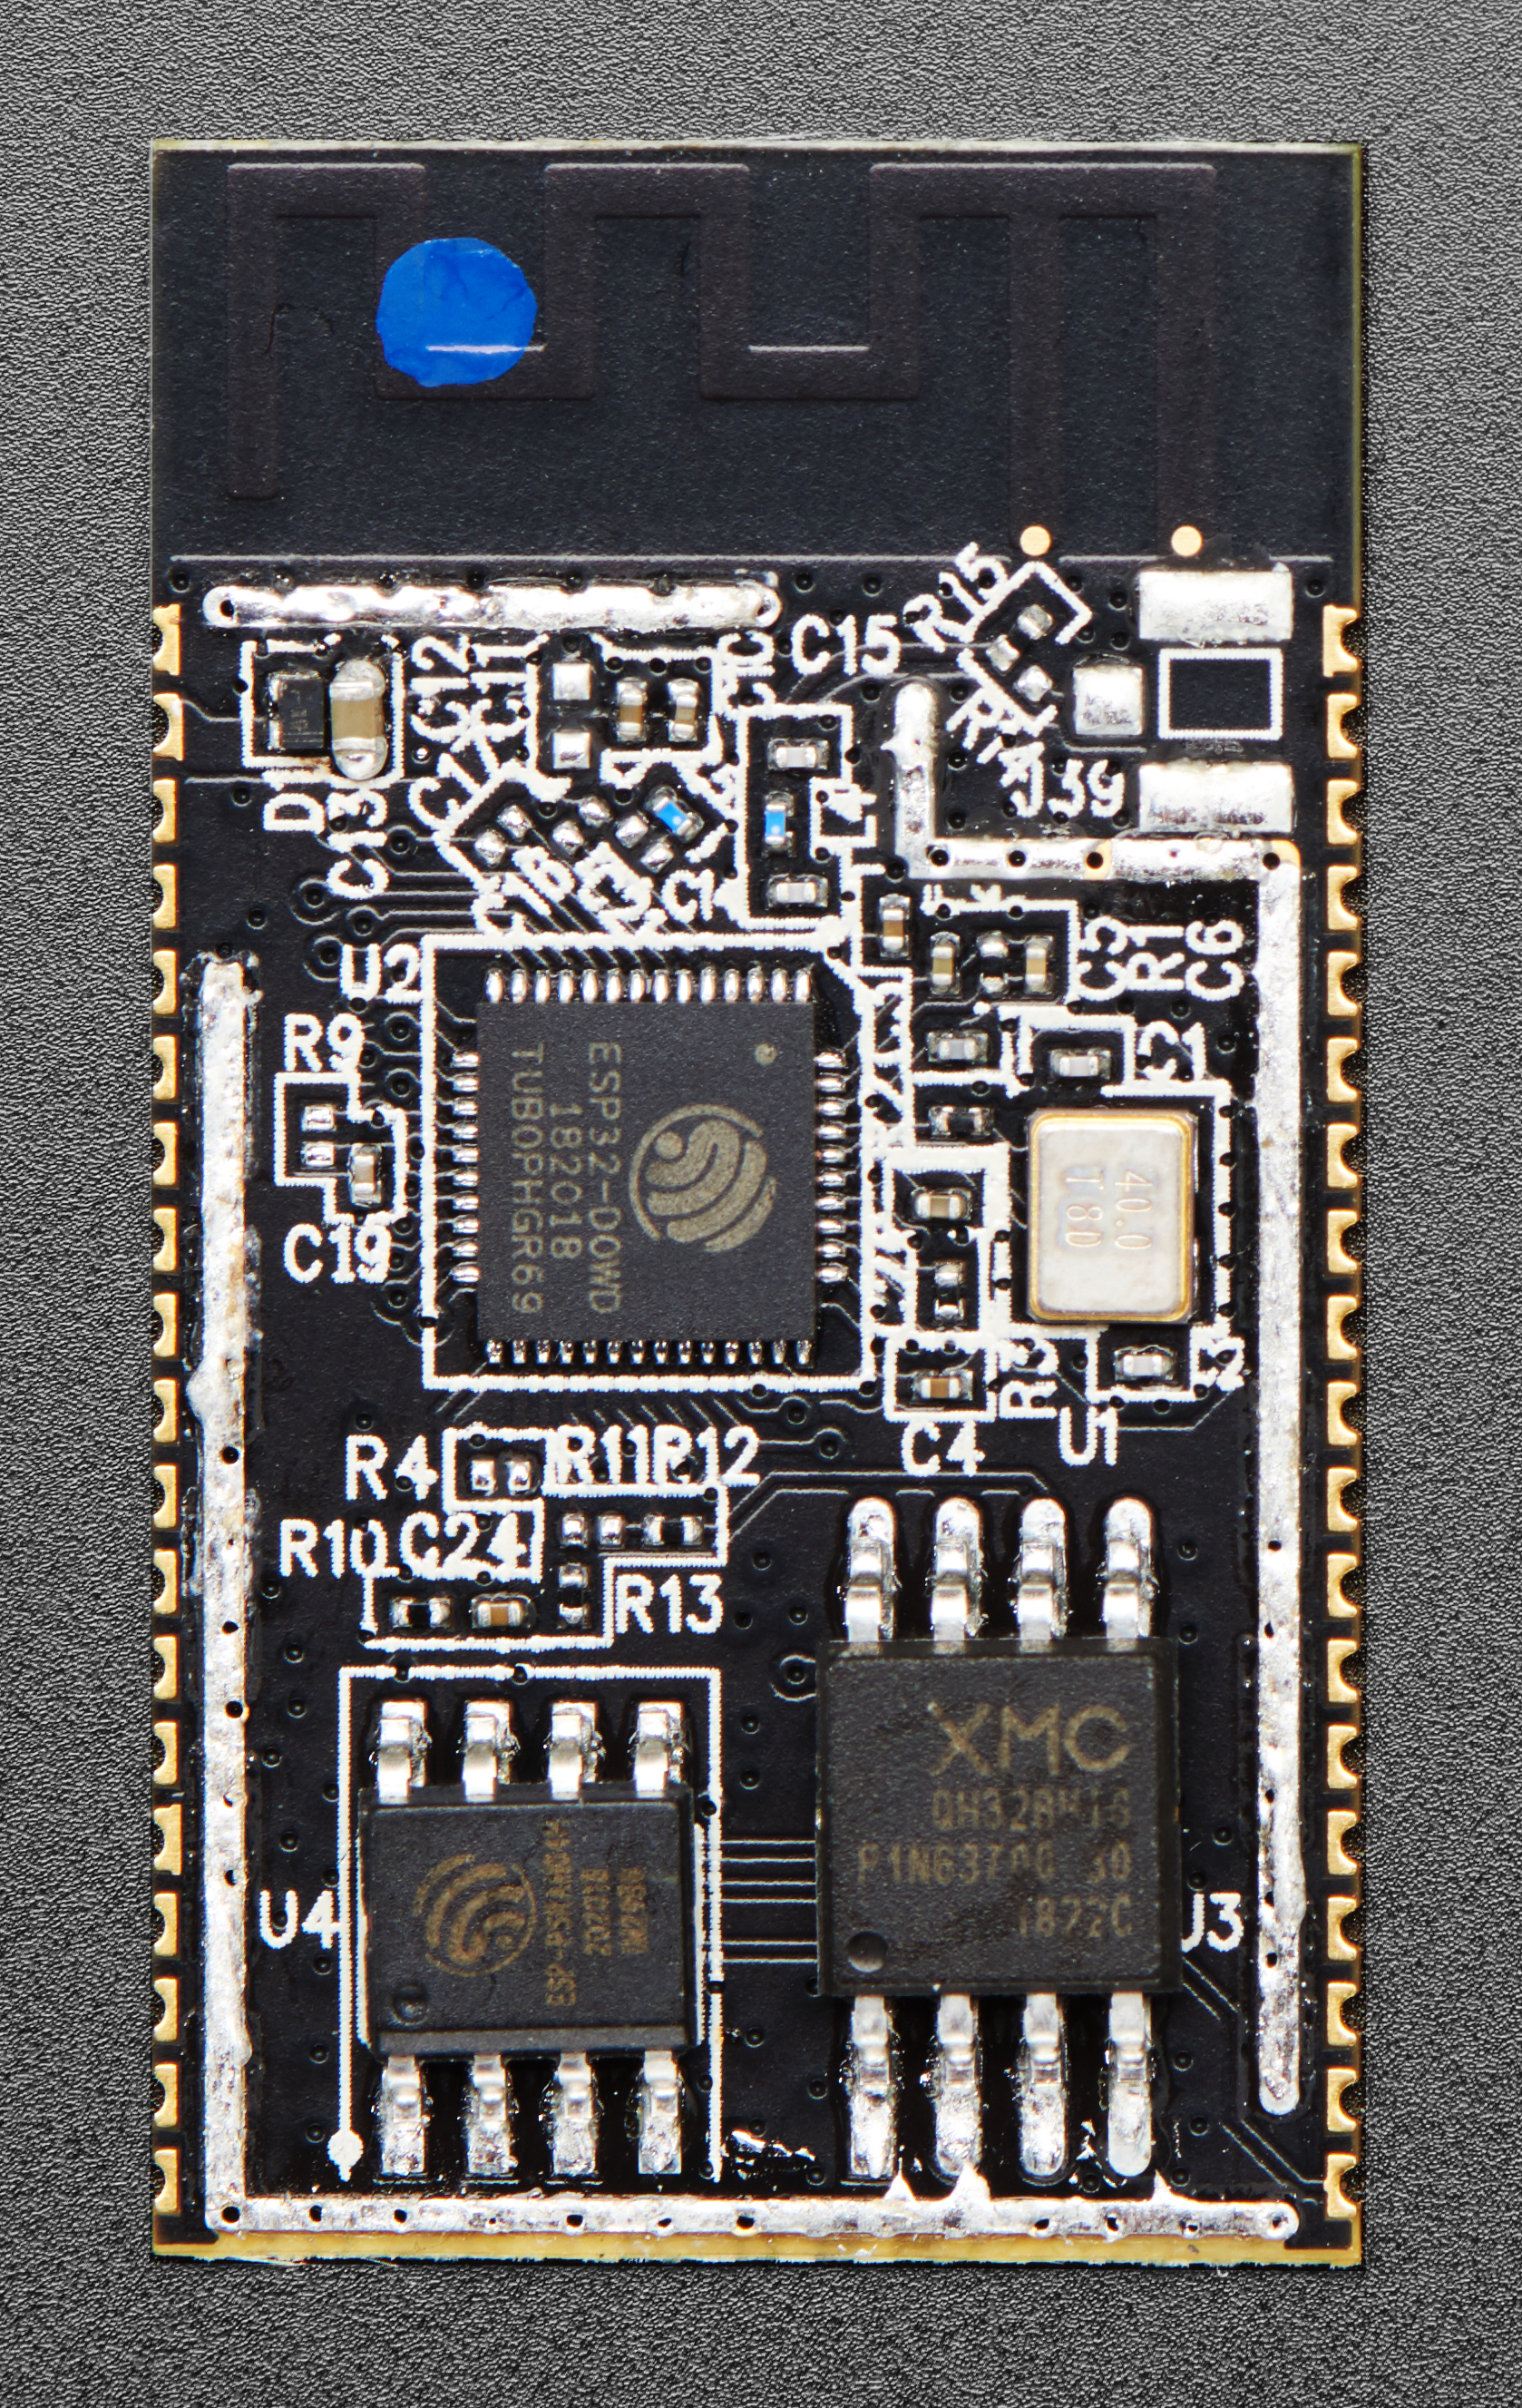
\includegraphics[width=.85\linewidth]{media/esp32_wrover_b.png}
            \subcaption{Foto di un modolo ESP32-WROVER-B basato sul chip ESP32 \parenciteit{}{ESP32_WROVER_B:Image}}
            \label{fig:ESP32_WROVER_B}
        \end{minipage}
        \hspace{.04\linewidth}
        \begin{minipage}[H]{.5\linewidth}
            \centering
            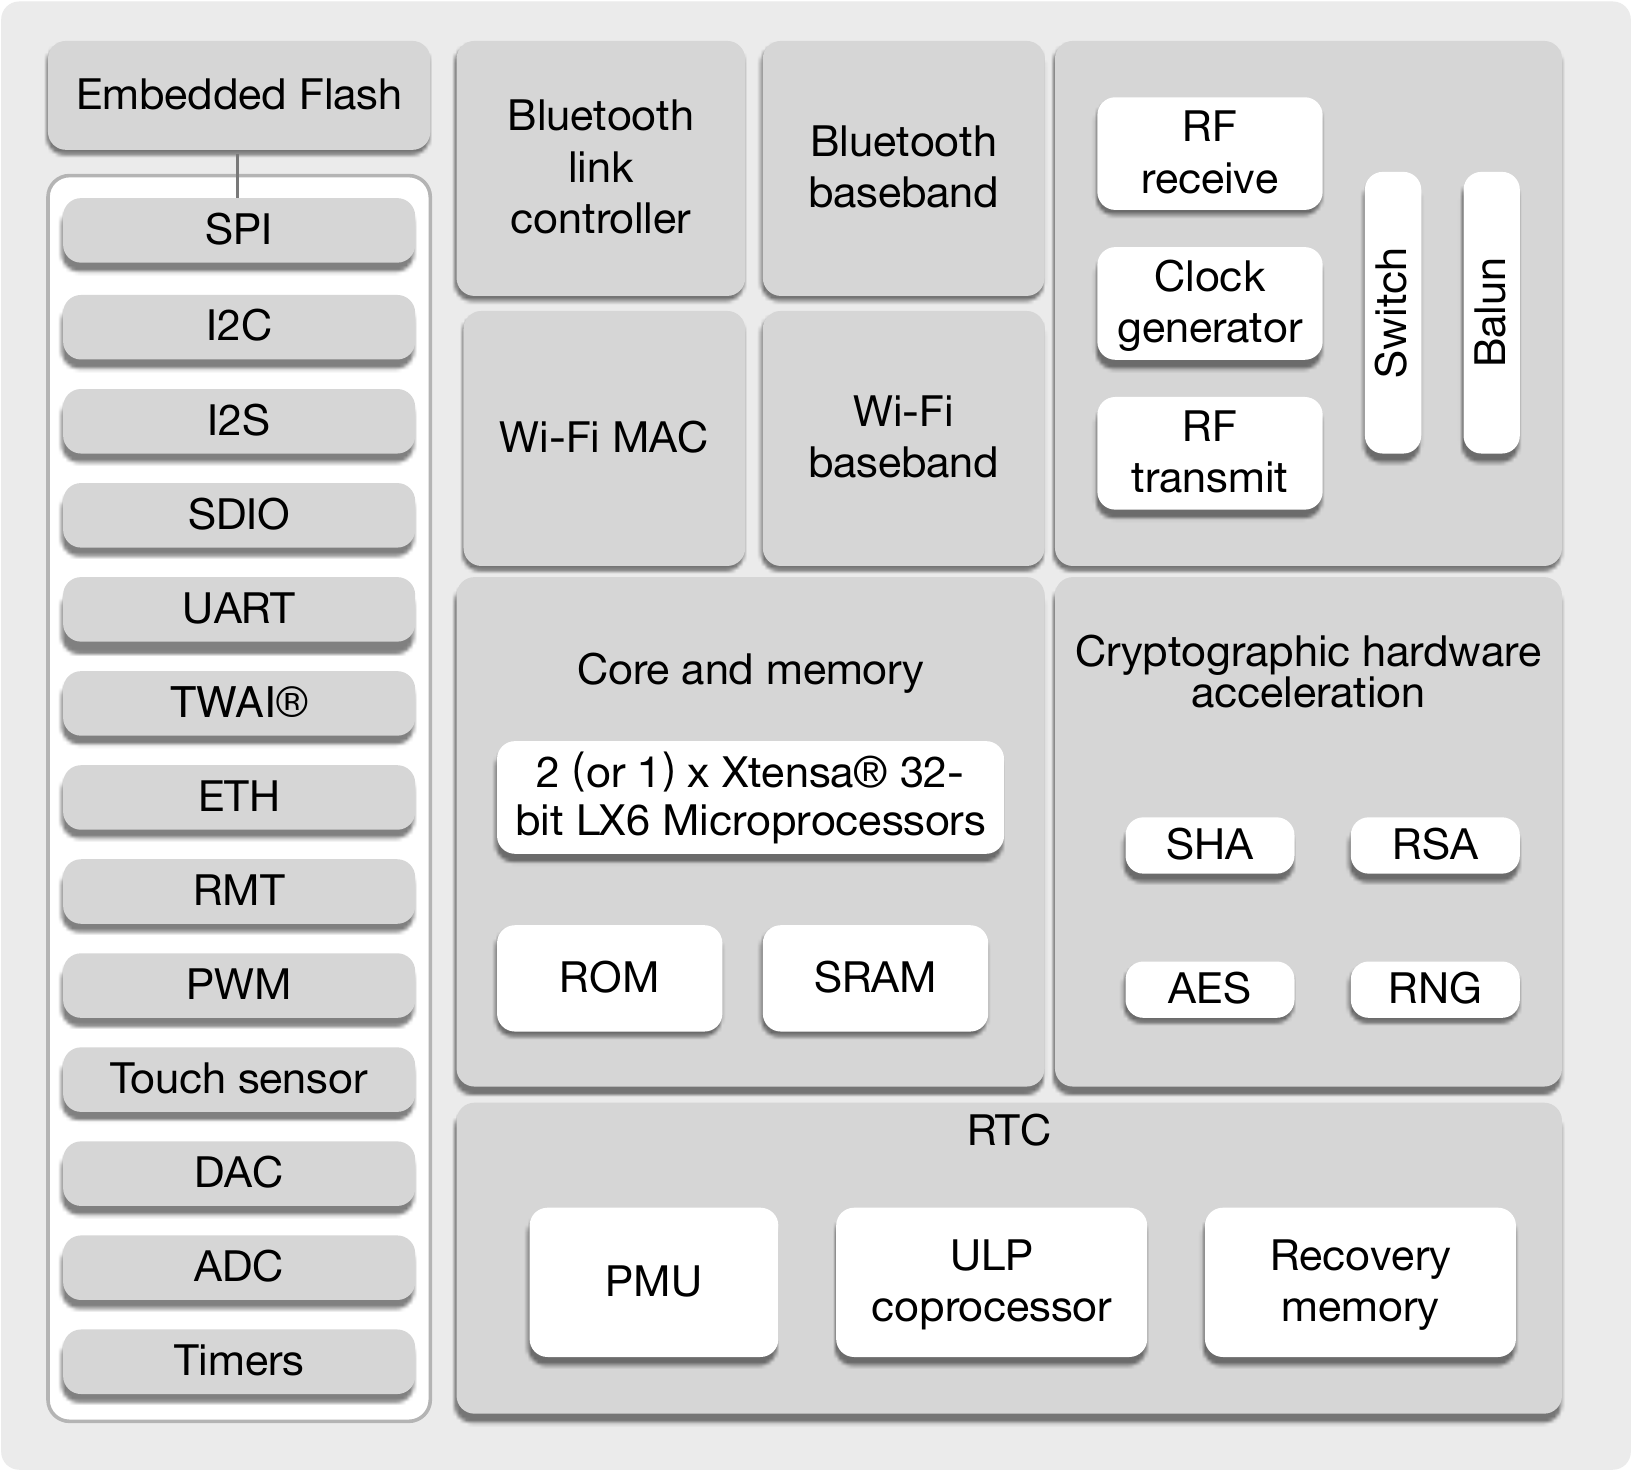
\includegraphics[width=\linewidth]{media/esp32_block_diagram.png}
            \subcaption{Diagramma a blocchi di un chip generico della linea ESP32 \parenciteit{p12}{ESP32:Datasheet}}
            \label{fig:ESP32_BD}
        \end{minipage}
        \caption{}
        \label{fig:ESP32}
    \end{figure}

    \begin{figure}[!htb]
        \centering
        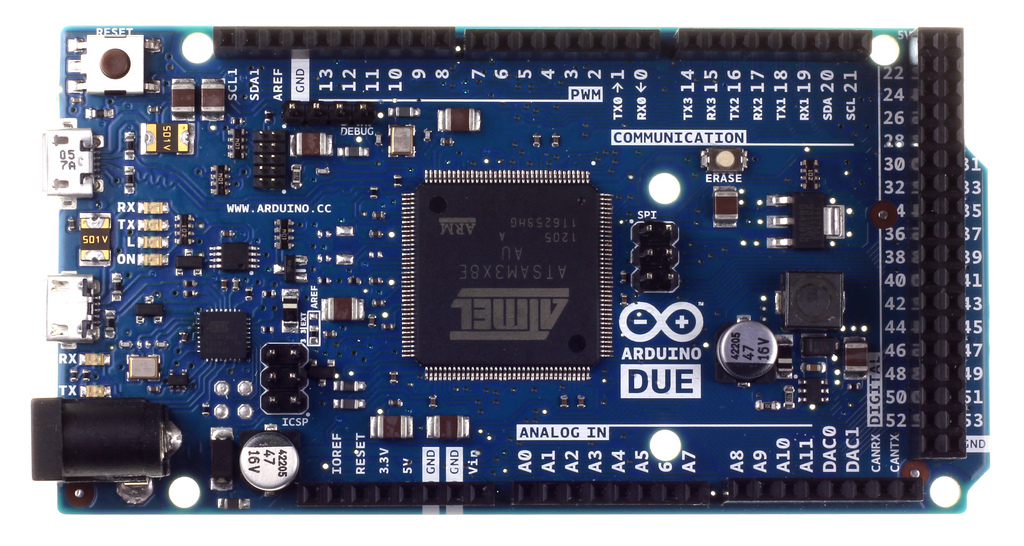
\includegraphics[width=.7\linewidth]{media/ArduinoDue_Front.jpg}
        \caption{Scheda Arduino Due \parenciteit{}{ArduinoDue:Image}}
        \label{fig:ArduinoDue}
    \end{figure}
    \clearpage
    \todo{search for all ?? references}
    \subsubsection{Alimentazione}\label{sec:MotherboardDesignSupply}
    L'alimentazione del circuito \`{e} una delle parti indispensabili ed importanti per il suo funzionamento corretto, soprattutto quando sono presenti circuiti analogici.
    Nel mio caso l'alimentazione deve avere la tensione costante nel tempo e deve possedere relativamente bassi livelli di rumori\footnote{La tensione deve essere costante e senza disturbi in tutte le possibili modalit\`{a} di operazione del circuito (ovvero con consumi differenti di corrente)}.
    Di conseguenza devo scegliere la topologia che creerebbe disturbi minimi mentre trasforma la tensione, che potrei applicare sia nella versione presente, sia nelle versioni future del prototipo.
    La migliore tecnica in assoluto per farlo \`{e} di utilizzare un regolatore lineare a principio di resistenza.
    Il motivo dietro la sua precisione \`{e}, che per abbassare la tensione al livello desiderato scarta la differenza necessaria sottoforma di calore: questo \`{e} l'effetto del clipping applicato al rumore contenuto nella sorgente\footnote{Si intende l'alimentazione del regolatore} a scapito della propria efficienza.

    La tensione delle sorgenti, che si tende anche a non modificare, deve essere tale per fornire la sua regolazione con un sistema poco complesso ed efficacie alimentato dalla batteria\footnote{Si intendono batterie Li-po che hanno delle tensioni minime (senza sovrascarica) di $3.6V$}, per permettere all'ADC di comunicare allo stesso livello di tensione della logica\footnote{Tensione alla quale adoperano le interfacce logiche del chip} dell'ESP32 di $3.3V$ e per alimentare l'ESP32 stesso.    
    Il quadro della situazione dell'utilizzo dei $3.3V$ si completa perfettamente con la decisione per il prototipo finale di una combinazione di un buck\footnote{Un circuito che riduce la tensione per via della propriet\`{a} dell'induttanza (con possibilit\`{a} di isolazione galvanica) con alta efficienza, a scapito del rumore ad alta frequenza che viente introdotto nel sistema, che aumenta con l'aumento del consumo della corrente} convertitore per rendere efficiente\footnote{}\todo{<-- add reference about efficency} la conversione della tensione dai $4.2V-3.6V$ ai approssimativi\footnote{Si dovr\`{a} concretizzare questa misura durante il design della sorgente del prototipo finale per le caratteristiche specifiche ai componenti scelti} $3.5V$ concatenato a dei regolatori lineari per eliminare il rumore introdotto dal nodo precedente\todo{<--add reference about reliability} e fornire i necessari $3.3V$.
    Questa decisione che ci guida alla conseguenza di poter utilizzare per il prototipo esclusivamente dei regolatori lineari per simulare\footnote{Per l'effetto del clipping dei regolatori lineari tendiamo a non percepire i rumori introdotti nella sorgente dai nodi precedenti (ovviamente i rumori che non vanno sotto il limite detto "dropout", dopo il quale i regolatori lineari smettono di mantenere tensione costante): di conseguenza si possono eliminare} la situazione finale del progetto e per ridurre la complessit\`{a} dei circuiti utilizzati.

    Nel caso concreto del prototipo, la sorgente positiva di tensione costante \`{e} gi\`{a} presente\footnote{La regolazione \`{e} di tipo resistivo lineare} nell'Arduino DUE, che viene alimentata dal cavo USB di $5V$ quando la scheda viene connessa al computer per la necessaria comunicazione di dati attraverso la porta seriale.
    La sorgente negativa, della quale avremo bisogno per i filtri\footnote{Vengono discussi i motivi nella Sezione\ref{sec:SensorBoardSchematic}}\todo{aggiungi che quando filtriamo dc, abbiamo un segnale con una parte negativa},viene data da un trasformatore\footnote{Figura \ref{fig:ProtoSupplyPhoto}} di $\Delta U = 12V$ senza connessione al \texttt{GND}\footnote{Si intende un conduttore che ha il potenziale $0V$ di riferimento} della presa, con isolazione galvanica dalla corrente della presa per riuscire a connetterla nel modo corretto senza causare corti-circuiti.
    In seguito la tensione viene ritotta con un regolatore resistivo lineare ai $3.3V$.
    Ci\`{o} mi permette creare due sorgenti di tensione di $3.3V$ e di $-3.3$ per via della connesione delle sorgenti in serie con un \texttt{GND} del circuito nel punto della loro connesione, come dimostrato nella Figura \ref{fig:ProtoSupplyConnection}.
    \begin{figure}[H]
        \centering
        \begin{minipage}{.44\linewidth}
            \centering
            \begin{tikzpicture}[transform shape, use fpu reciprocal]
                \draw (0,0)
                    node[above]{$U_{+}$}
                    to[short, o-] ++(0,0)
                    ++(0,-2)
                    to[V=$5V$, l_=$V_1$] ++(0,2)
                    ++(0,-2)
                    coordinate(joint)
                    to[short, -o] ++(1,0)
                    node[right]{$U_{GND}$}
                    (joint) 
                    ++(0,-2)
                    to[V=$12V$, -*, l_=$V_2$] ++(0,2)
                    ++(0,-2)
                    to[short, o-] ++(0,0)
                    node[below]{$U_{-}$};
            \end{tikzpicture}
            \subcaption{Sorgenti $V_1$ e $V_2$ sono connessi in serie con \texttt{GND} al loro centro per fornire $\Delta U_{GND\rightarrow +}=5V$ $\Delta U_{GND\rightarrow -}=-12V$}
            \label{fig:ProtoSupplyConnection}
        \end{minipage}
        \hspace{.04\linewidth}
        \begin{minipage}[H]{.44\linewidth}
            \centering
            % [2026 revision] replaced 4608x2229 prototype-era snapshot with a clean photo of the
            % 12V charger (was: media/album/PSX_20220227_234319.jpg — kept on disk unchanged)
            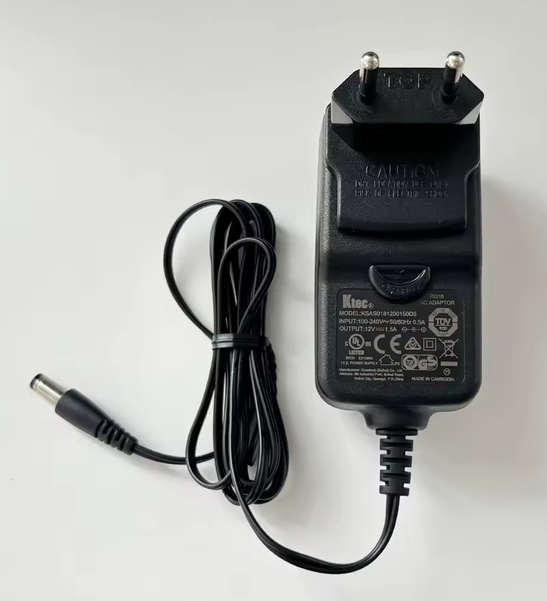
\includegraphics[width=\linewidth]{media/album/12v-charger.jpg}
            \subcaption{Alimentatore che uso per trasformare la tensione in $12V$ dalla tensione della presa con corrente massima di $500mA$}
            \label{fig:ProtoSupplyPhoto}
        \end{minipage}
        \caption{}
        \label{fig:ProtoSuppy}
    \end{figure}
    \clearpage

    \noindent Il circuito che uso per ridurre la tensione dai $12V$ ai $3.3V$ \`{e} nella seguente Figura:
    \begin{figure}[H]
        \centering
        \begin{minipage}[H]{.44\linewidth}
        \centering
        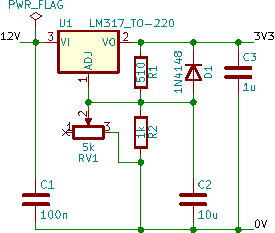
\includegraphics[page=1, width=\linewidth]{media/power_source_board_pcb_cropped.pdf}
        \subcaption{Diagramma del circuito composto nel software KiCad \parenciteit{}{KiCad:Software}, dove attraverso il potenziometro $RV1$ si pu\`{o} variare la tensione di uscita \emph{(Il circuito \`{e} stato progettato in vista del riuso coi prototipi futuri, per questo ci sono condensatori bypass $C1$ \& $C3$, di cui ne parlo nella Sezione \ref{sec:SensorBoardSchematic}, e il diodo $D1$ con il condensatore $C2$ per proteggere dai corti-circuiti)} \emph{(Parzialmente preso da \cite[p9]{LM317:Datasheet})}}
        \label{fig:PowerSourceBoardSchematic}
        \end{minipage}
        \hspace{.04\linewidth}
        \begin{minipage}[H]{.45\linewidth}
            \centering
            \begin{minipage}[H]{\linewidth}
                \centering
                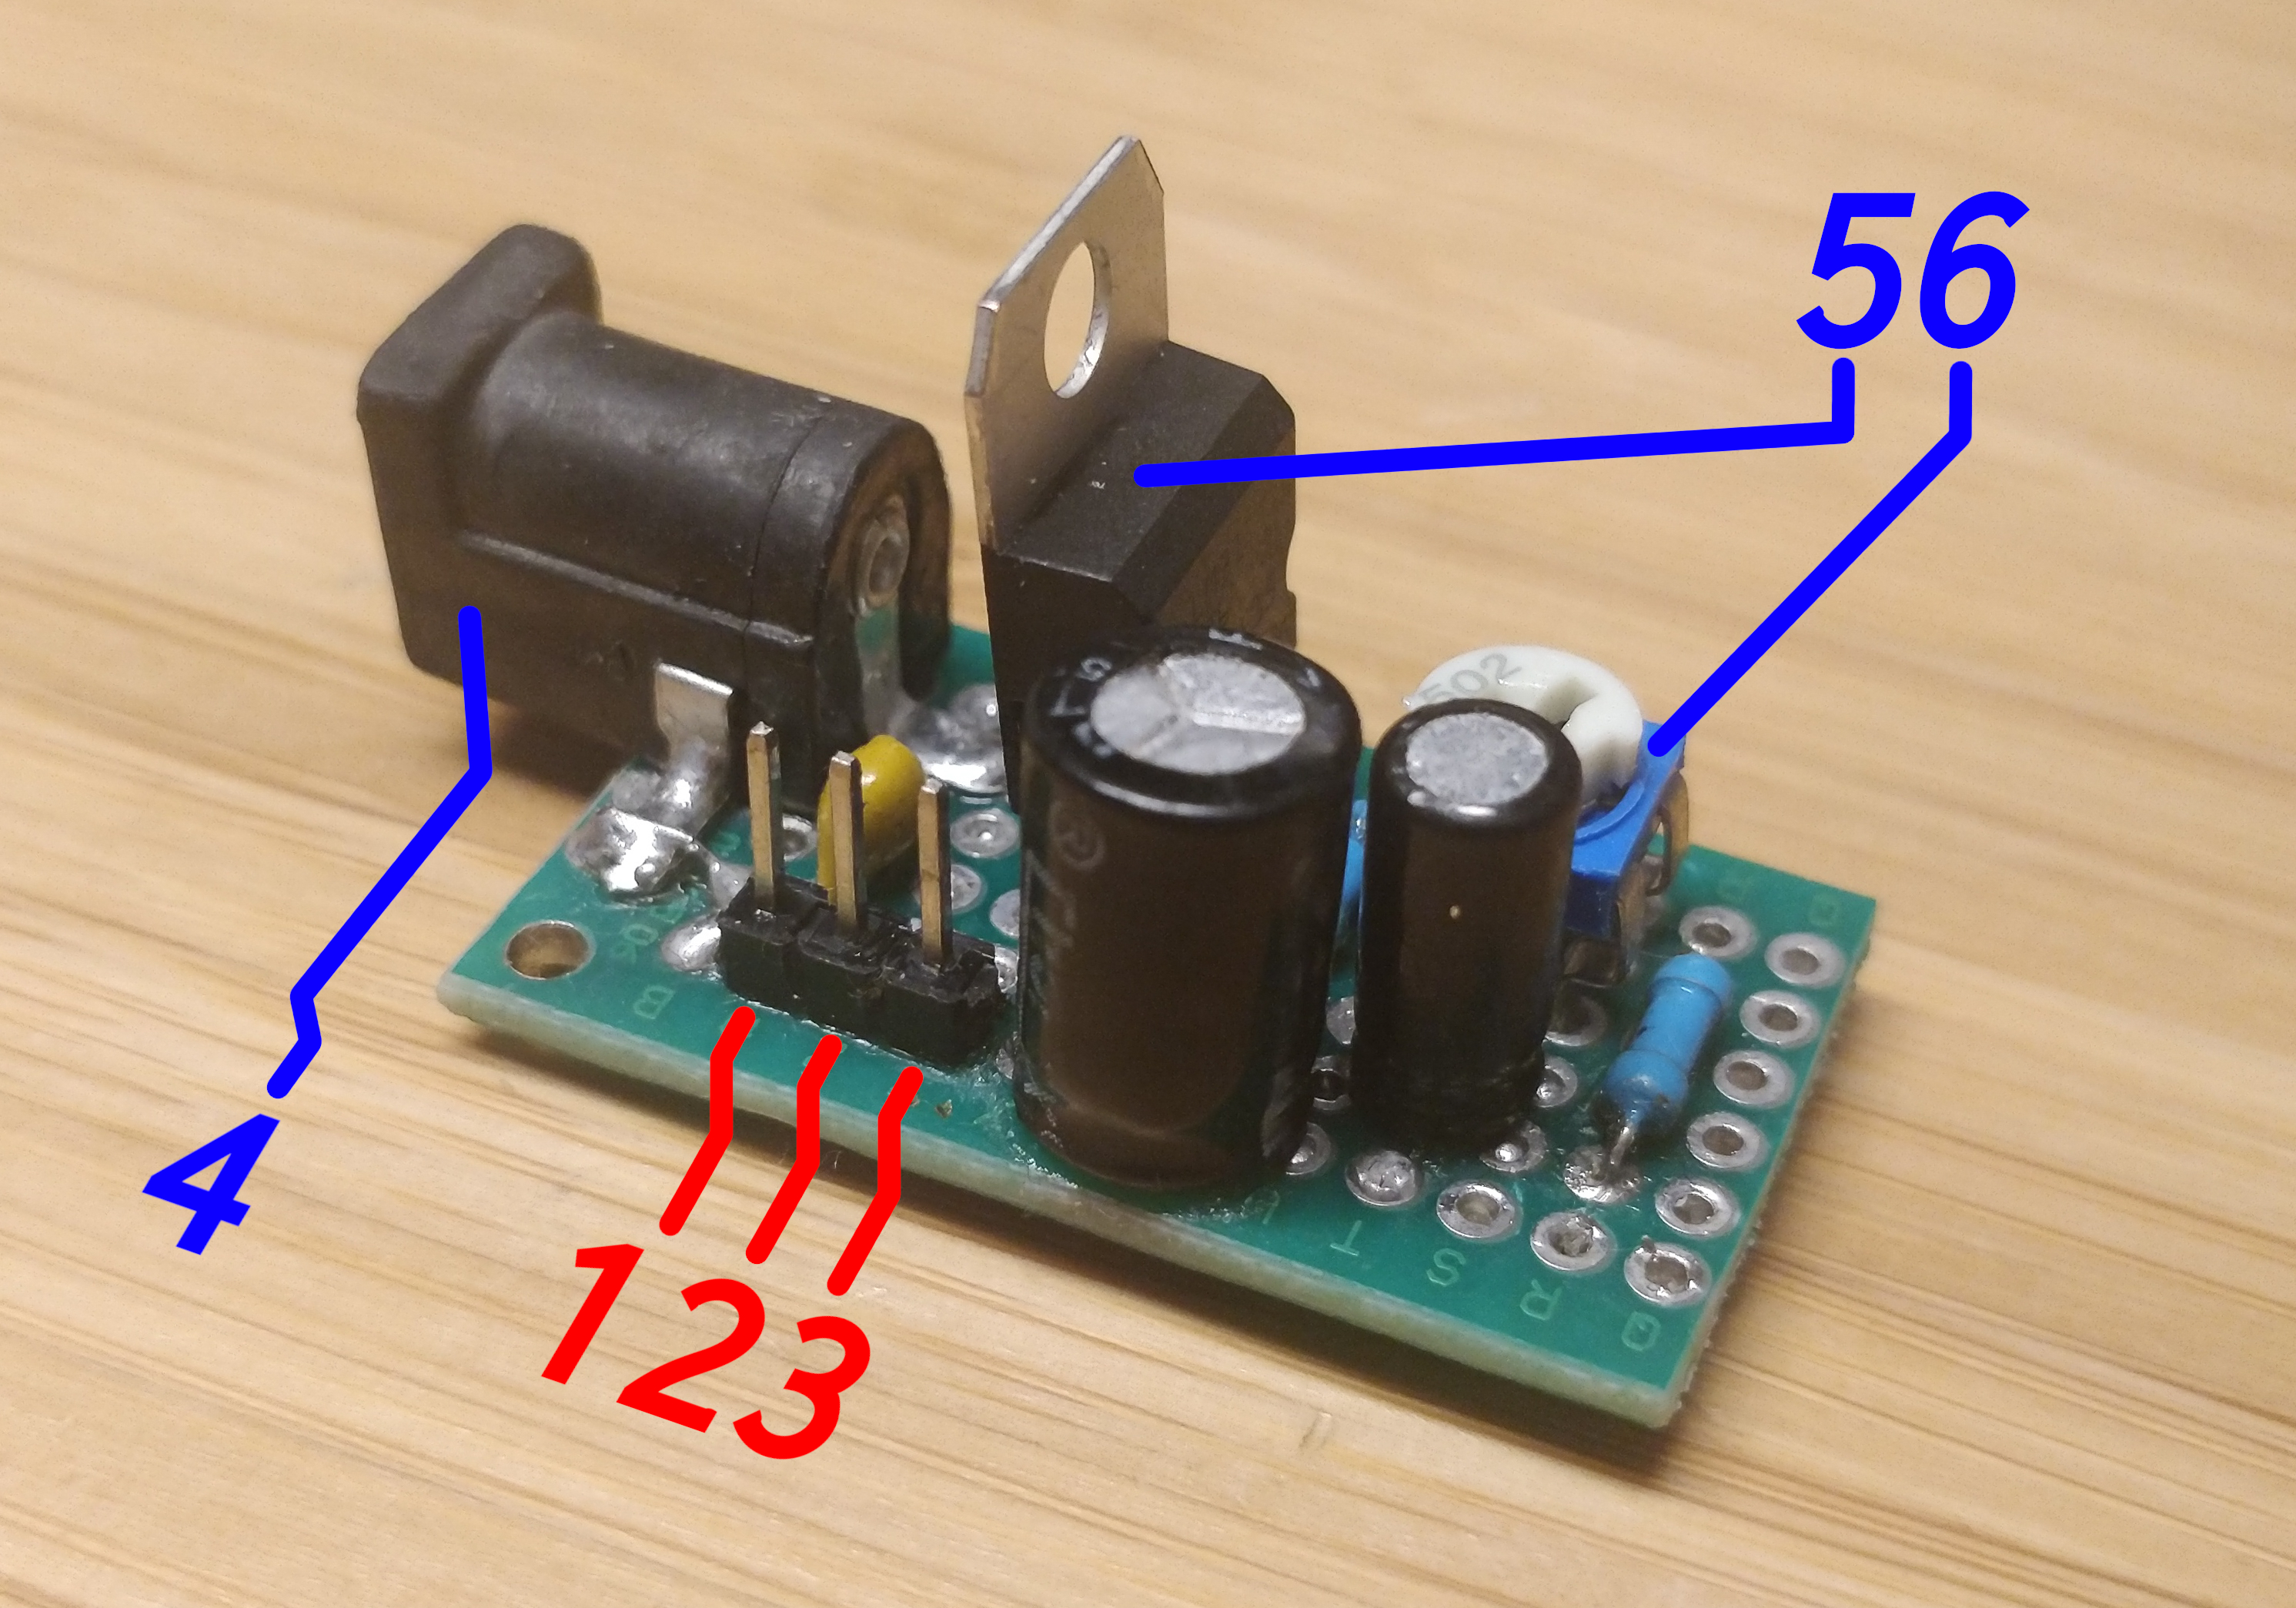
\includegraphics[width=.66\linewidth]{media/album/PSX_20220227_234533_ed.jpg}
                \subcaption{Scheda del regolatore e le sue componenti. In rosso: $1$ - pin $0V$, $2$ - pin $12V$, $3$ - pin $3V3$. In blu: $4$ - connettore per l'alimentatore, $5$ - LM317, $6$ - potenziometro $RV1$ \emph{(Al momento della costruzione non avevo il condensatore di tipo ceramico $C3$ e l'ho sostituito con un tipo elettrolitico)}}
                \label{fig:PowerSourceBoardPhoto}
            \end{minipage}
            \\
            \begin{minipage}[H]{\linewidth}
                \centering
                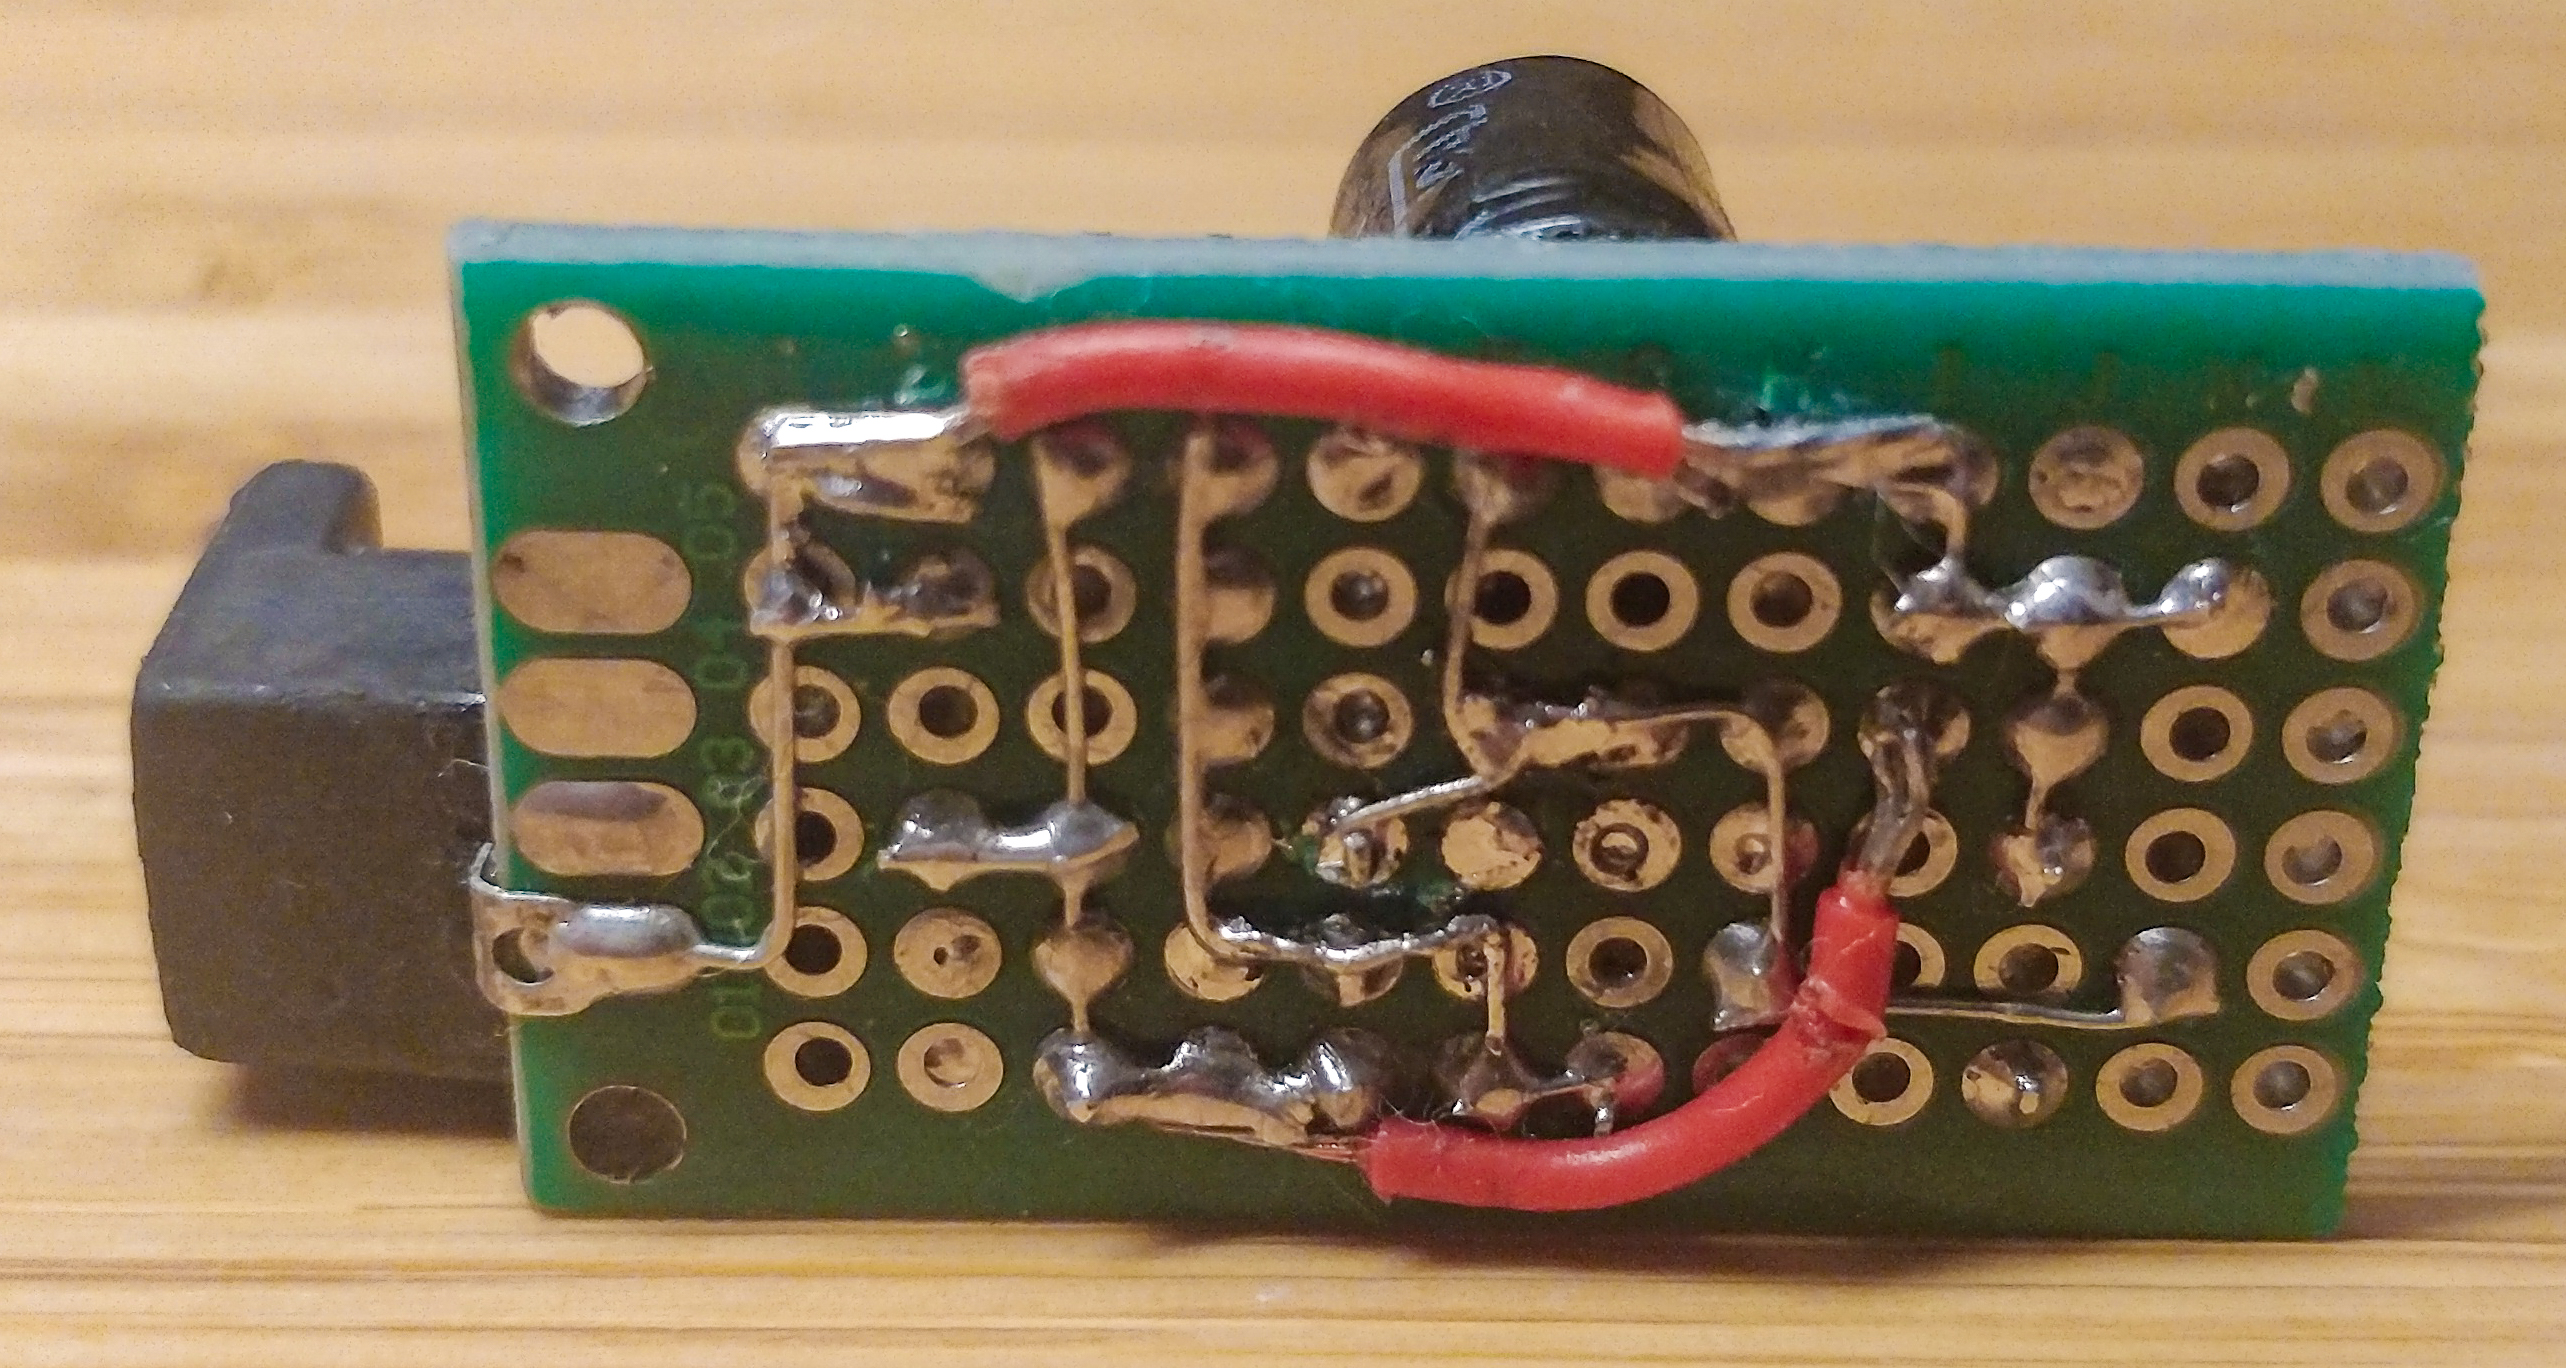
\includegraphics[width=.8\linewidth]{media/album/PSX_20220227_234420.jpg}
                \subcaption{Connessioni del componenti sul retro della scheda del regolatore: il circuito \`{e} stato saldato con THT \emph{(Through Hole Tecnology, ovvero tecnologia attraverso i fori)} per ridurre tempo speso sulla proggettazione, costruzione}
                \label{fig:PowerSourceBoardPhotoBack}
            \end{minipage}
        \end{minipage}
        \caption{Scheda del regolatore lineare aggiustabile ai $1.25V-3.375V$ basata su LM317 \parenciteit{}{LM317:Datasheet}}
        \label{fig:PowerSourceBoard}
    \end{figure}
    \todo{aggiungi riferenza su github del progetto}
    \noindent I conti necessari per determinare le resistenze sono i seguenti:
    
    \begin{figure}[H]
        \centering
        \begin{minipage}[H]{.15\linewidth}
            \[U_{out} \approx 3.3V\]
        \end{minipage}
        \begin{minipage}[H]{.15\linewidth}
            \[U_{ref}=1.25V\]
        \end{minipage}
        \begin{minipage}[H]{.15\linewidth}
            \[R_2=1k\Omega\]
        \end{minipage}
        \begin{minipage}[H]{.15\linewidth}
            \[RV_1=5k\Omega\]
        \end{minipage}
        \begin{minipage}[H]{.15\linewidth}
            \[I_{adj}=100\mu A\]
        \end{minipage}
        \begin{minipage}[H]{\linewidth}
            \vspace{3ex}
            \[U_{out}=U_{ref}\left(1+\frac{RV_1 \parallel R_2}{R_1}\right)+I_{adj} \left(RV_1 \parallel R_2\right)\]
        \end{minipage}
    \end{figure} \todo{aggiungi riferimento a come si fa a fare il segno parallele nel circuito}
    \noindent $I_{adj}$ \`{e} la corrente che fluisce attraverso il pin \texttt{ADJ} del regolatore LM317, che come si vede ha influsso sull'$U_{out}$, che con la scelta equilibrata dei valori delle resistenze e tende ad essere piccolo.
    I valori delle resistenze sono da scegliere in base alla scala dei valori standardizzati serie E\footnote{I valori si applicano non solo alle resistenze, ma anche ai condensatori}\:\footcite[]{ESeries:Wiki}.
    Dopo un po'di ricerca di componenti che avevo gi\`{a} a disposizione e un po'di tentativi con i calcoli sono arrivato ai valori\footnote{I valori dei condensatori sono stati presi direttamente dalla sorgente del diagramma nella Figura \ref{fig:PowerSourceBoardSchematic}} che si vedono nel diagramma del circuito nella Figura \ref{fig:PowerSourceBoardSchematic}.
    \clearpage

    \section{Filtri - Teoria}\label{sec:FilterTheory}
    Sotto il termine "filtri", tenendo conto anche del contenuto della Sezione \ref{sec:SensorboardDesignInput} e della Sezione \ref{sec:SensorboardDesignOutput}, si intendono i filtri di frequenza, che comodamente\footnote{Si discute il motivo nella Sezione \ref{sec:ElectronicsCalculusLaplace}} fanno parte dei sistemi LTI\footnote{Si discute del termine e il suo significato nella prossima Sezione, Sezione \ref{sec:FilterTheorySystems}}.

    \subsection{Sistemi}\label{sec:FilterTheorySystems}
    Quando menziono \emph{Input} ed \emph{Output}, mi riferisco al concetto dei sistemi dato dalla teoria dei sistemi e del controllo\footcite[]{ControlTheory:Wiki}.
    La teoria, nel nostro caso, risulta utile perch\'{e} fornisce un modello, attraverso il quale possiamo progettare un sistema\footnote{Il sistema inizialmente \`{e} un concetto astratto di un soggetto che elabora delle entrate dando delle uscite, il quale in seguito \`{e} possibile implementare} che ci permetterebbe di raggiungere dei desiderati stati di qualche numero di \emph{Output} attraverso dei stati di qualche numero di \emph{Input} in modo pi\`{u} ottimale possibile.

    \begin{samepage}
        \noindent Esistono diverse categorie dei sistemi date dalle loro caratteristiche, ma noi siamo interessati solo di una specifica, nella quale entra il nostro filtro:
        \begin{enumerate}[label=\emph{(\arabic*)}]
            \item Tipologia dell'interfaccia: SISO, ovvero Single Input Single Output\footnote{Unica Entrata Unica Uscita}
            \item Tipologia del sistema: LTI, ovvero Linear Time Invariant\footnote{Lineare Invariante nel Tempo}
        \end{enumerate}
    \end{samepage}
    Il nome della prima caratteristica parla per se stesso, mentre la seconda caratteristica pu\`{o} parere meno chiara.
    I due concetti che racchiude l'LTI, linearit\`{a} ed invarianza nel tempo, devono essere discussi.

    A s\'{e}, la caratteristica della linearit\`{a}, si pu\`{o} presentare in diversi sistemi se non utilizzati al loro limite fisico al quale sono stati progettati anche se, prevalentemente, i sistemi nel mondo reale sono tendenzialmente non-lineari\footcite[]{TransferFunction:Wiki}.
    \begin{samepage}
        \noindent Concretizzando, il concetto della linearit\`{a} \`{e} descritto dalla soddisfazione di due condizioni:
        \begin{enumerate}[label=\emph{(\arabic*)}]
            \item Additivit\`{a}, descritta dalla seguente formula: \[f(x + y) = f(x) + f(y)\]
            \item Omogeneit\`{a}, descritta dalla seguente formula: \[f(a \cdot x) = a \cdot f(x)\]
        \end{enumerate}
    \end{samepage}

    Un esempio reale di un sistema lineare pu\`{o} essere un circuito, come nella Figura \ref{fig:ExampleLTICircuit}, contenente un transistor\footnote{Nel caso dell'esempio consideriamo un MOSFET}, l'\emph{Output} del quale si comporter\`{a} nel modo lineare\footnote{Si pu\`{o} vedere nella Figura \ref{fig:ExampleLTIIRFZ44N_Plot_Vgs}} con la variazione della tensione\footnote{Il fenomeno avviene coi MOSFET, ma non tutti i transistor funzionano allo stesso modo} all'\emph{Input} se \`{e} operato nel regime di saturazione.
    Il regime di saturazione, che si pu\`{o} identificare nella Figura \ref{fig:ExampleLTIIRFZ44N_Plot_Vds}, \`{e} una gamma di tensioni $U_{out}$ (corrispondente al $V_{DS}$) per $V_{DS_{saturazione}} < V_{DS}$ per le quali il transistor si comporta linearmente con la variazione della tensione $U_{in}$\footnote{Deve essere presa in considerazione anche lei perch\'{e} \`{e} un parametro della funzione presentata nel grafico: aumentando il $V_{GS}$, aumenta la tensione $V_{DS_{saturazione}}$} (corrispondente al $V_{GS}$).
    Se il circuito, invece, viene adoperato nel regime tripole, la gamma di $V_{DS}$ per $0 < V_{DS} < V_{DS_{saturazione}}$, l'$I_D$ inizia a dipendere anche da $V_{DS}$ o $U_{out}$: con questo comportamento il circuito viola le due condizioni definite dal comportamento lineare, in tale modo rendendosi un sistena non-lineare.
    \begin{figure}[H]
        \centering
        \begin{minipage}{.84\linewidth}
            \centering
            \begin{tikzpicture}[transform shape, use fpu reciprocal]
                \draw (0,0)
                    node[above]{$U_{+}$}
                    to[short, o-] ++(0,-.25)
                    to[R, l=$R$, -*] ++(0,-2)
                    coordinate(joint)
                    to[short, -o] ++(1,0)
                    node[right]{$U_{out}$}
                    (joint) to[short] ++ (0,-.5)
                    node[nigfete, anchor=D, bodydiode, tr circle] (fet) {$Q$}
                    (fet.S) node[anchor=south east] {\footnotesize{\texttt{S}}}
                    (fet.D) node[anchor=north east] {\footnotesize{\texttt{D}}}
                    (fet.G) node[anchor=south west] {\footnotesize{\texttt{G}}}
                    (fet.S) node[ground]{} ++(0,-.5)
                    (fet.G) to[short, -o] ++(-.5,0)
                    node[left]{$U_{in}$};
            \end{tikzpicture}
            \subcaption{IRFZ44N si nomina $Q$ \emph{(}\texttt{G}\emph{ = Gate, }\texttt{D}\emph{ = Drain, }\texttt{S}\emph{ = Source)}, una resistenza ideale $R$, sorgente di tensione costante $U_{+}$, l'\emph{Input} $U_{in}$ e l'\emph{Output} $U_{out}$}
            \label{fig:ExampleLTICircuit}
        \end{minipage}
        \\
        \vspace{3ex}
        \begin{minipage}[t]{.4\linewidth}
            \centering
            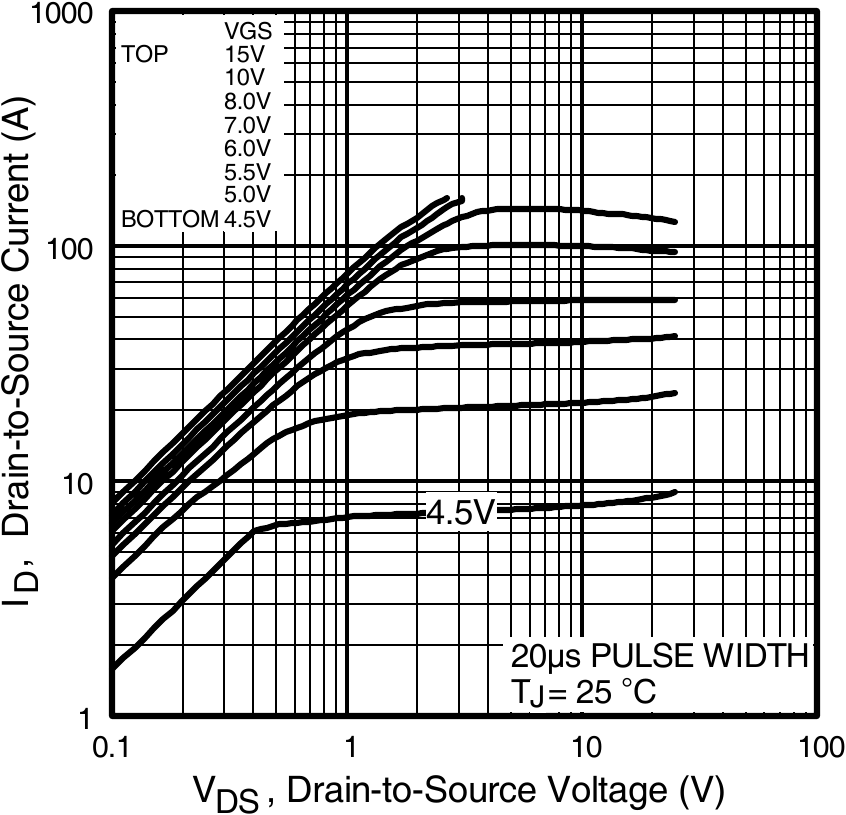
\includegraphics[width=\linewidth]{media/irfz44n_vds_id_plot.png}
            \subcaption{Variazione dell'$I_D$ in funzione al $V_{DS}$ con parametro $V_{GS}$ \emph{(il regime di saturazione \`{e} definito per $V_{DS}$ dopo la approssimativa cessazione di crescita di $I_D$)}}
            \label{fig:ExampleLTIIRFZ44N_Plot_Vds}
        \end{minipage}
        \hspace{.04\linewidth}
        \begin{minipage}[t]{.4\linewidth}
            \centering
            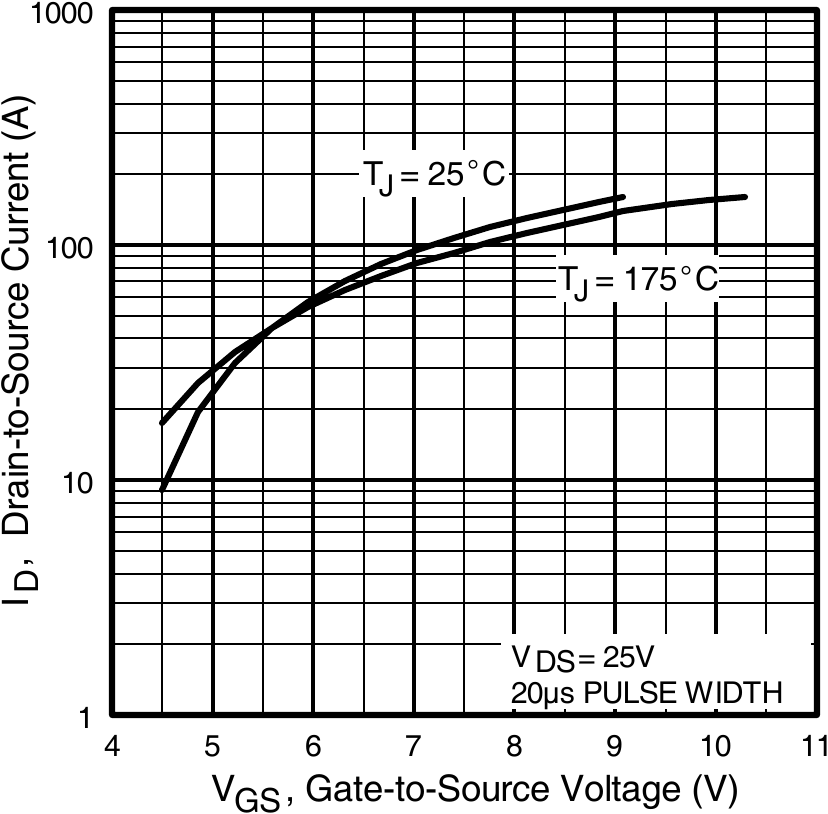
\includegraphics[width=\linewidth]{media/irfz44n_vgs_id_plot.png}
            \subcaption{Variazione dell'$I_D$ in funzione al $V_{GS}$ nel regime di saturazione per \emph{($V_{DS} = 25V$)}, che \`{e} approssimativamente lineare}
            \label{fig:ExampleLTIIRFZ44N_Plot_Vgs}
        \end{minipage}
        \caption{Esempio di un amplificatore a base di un IRFZ44N \emph{(Un transisor, se piu specifico, un MOSFET di tipo N-canale di modalit\`{a} Enhancement)} \parenciteit{}{IRFZ44N:Datasheet} con rispettivo circuito in \ref{fig:ExampleLTICircuit} e i grafici \parenciteit{}{IRFZ44N:Datasheet} delle Volt-Amper caratteristiche in \ref{fig:ExampleLTIIRFZ44N_Plot_Vds}, \ref{fig:ExampleLTIIRFZ44N_Plot_Vgs}}
        \label{fig:ExampleLTI}
    \end{figure}


    Il concetto dell'invarianza nel tempo \`{e} dato dalla consistenza dei risultati nel tempo del sistema: il sistema non deve dare diversi \emph{Output} per medesimi \emph{Input} in momenti distinti per essere considerato invariante nel tempo.

    Un bell'esempio del sistema variante nel tempo potrebbe essere un sito-web che serve a far vedere fusi orari in tempo reale.
    Se viene richiesta la data e il tempo di un preciso fuso orario, ogni volta i valori ricevuti saranno diversi da quelli richiesti in un prossimo momento.


    I motivi per i quali il filtro di frequenze analogico a noi necessario si considera un sistema LTI, sono per la propriet\`{a} dei circuiti analogici di tendere a descrivere facilmente determinati sistemi invarianti nel tempo\footnote{La varianza nel tempo di un sistema elettronico progettato ad essere invariante, come la linearit\`{a}, pu\`{o} dipendere da fenomini fisici come variazione di resistenza a temperature diverse, oppure le EMI} ed essere lineari nella loro risposta se non utilizzati fuori dai parametri porgettati, come la tensione di saturazione dei MOSFET nell'esempio precedente.
    Un'informazione aggiuntiva sarebbe che la varianza nel tempo pu\`{o} avere senso nei termini dell'elaborazione del segnale quando si usano sistemi digitali, dove i dati non sono strettamente legati al tempo, ma sono discreti.

    Il vero vantaggio di avere classificato il fitro sotto i sistemi LTI si nota quando si riescono a capire le loro propriet\`{a}\footnote{Le propriet\`{a} e le relazioni tra loro sono discusse nella Sezione \ref{sec:TransformsAndLaplace}}, che sono la possibilit\`{a} di descrivere il sistema con un impulso e la diretta conseguenza di questo primo fatto, il poter rappresentare il sistema con una funzione, detta funzione di trasferimento.
    \clearpage

    \subsection{Matematica \& Fisica} \label{sec:MathAndPhysics}
    Ho accenato delle funzioni di trasferimento\footcite[]{TransferFunction:Wiki} nelle sezioni\footnote{Sezione \ref{sec:IntroFiltersSignals} e Sezione \ref{sec:FilterTheorySystems}} precedenti e della loro caratteristica di essere un'astrazione del filtro.
    \begin{samepage}
        Si deve tenere conto delle seguenti uguaglianze:
        \begin{figure}[H]
            \centering
            \begin{minipage}[b]{.35\linewidth}
                \centering
                \[
                    H(s) = \frac{Output}{Input} = \frac{U_{out}}{U_{in}}
                \]
            \end{minipage}
            \begin{minipage}[b]{.35\linewidth}
                \centering
                \[
                    s = j\omega\ + \sigma
                \]
            \end{minipage}
        \end{figure}
    \end{samepage}

    Le funzioni di trasferimento, generalmente indicate con la lettera maiuscola $H(s)$ con una notazione della funzione matematica, sono delle funzioni che descrivono la relazione di un dominio, ovvero \emph{Input}, e un codominio, ovvero \emph{Output}, in funzione della variabile complessa $s$ mettendo in relazione l'\emph{Input} e l'\emph{Output} per via della divisione dell'uno per l'altro.
    Inoltre, sapendo che il segnale che stiamo studiando \`{e} descritto da variazioni di tensione, facciamo corrispondere l'\emph{Input} a $U_{in}$ e l'\emph{Output} a $U_{out}$.

    In termini di fisica e matematica sappiamo che $j$, che nel nostro caso rappresenta il valore immaginario della \(i\), viene moltiplicato per $\omega$ costituendo in tale modo la parte immaginaria dell'$s$ a condizione di $\Im(\omega) = 0$.
    La \(\sigma\), invece, costituisce la parte reale della \(s\), sempre tenendo conto dell'identica condizione $\Im(\sigma) = 0$.

    \noindent Una funzione di trasferimento \`{e} descrivibile anche da due polinomi $N_n(x)$ al numeratore e $D_m(y)$ al denominatore nel modo seguente:
    \begin{figure}[H]
        \centering
        \begin{minipage}[b]{.3\linewidth}
            \centering
            \[
                N_n(x) = \sum^{n}_{k=0} a_k x^k \mathrm{,}
            \]
        \end{minipage}
        \begin{minipage}[b]{.3\linewidth}
            \centering
            \[
                D_m(y) = \sum^{m}_{j=0} b_j y^j \mathrm{,}
            \]
        \end{minipage}
        \begin{minipage}[b]{.3\linewidth}
            \centering
            \[
                H(s) = \frac{N_n(s)}{D_m(s)}
            \]
        \end{minipage}
    \end{figure}
    \noindent Allora $H(s)$ pu\`{o} essere riscritta con polinomi in forma espansa o fattorizzata
    \begin{figure}[H]
        \centering
        \begin{minipage}[b]{.45\linewidth}
            \centering
            \[
                H(s) = \frac{a_0 + a_1 s + \dotsm + a_{n-1} s^{n-1} + a_n s^n}{b_0 + b_1 s + \dotsm + b_{m-1} s^{m-1} + b_m s^m} \mathrm{,}
            \]
        \end{minipage}
        \hspace{0.04\linewidth}
        \begin{minipage}[b]{.45\linewidth}
            \centering
            \[
                H(s) = \frac{z_0 \left(s - z_1\right) \dotsm \left(s^{n-1} - z_{n-1}\right) \left(s^n - z_n\right)}{p_0 \left(s - p_1\right) \dotsm \left(s^{m-1} - p_{m-1}\right) \left(s^m - p_m\right)}
            \]
        \end{minipage}
    \end{figure}
    \noindent e sostituendo nell'uguaglianza la seguente espressione $K = \frac{z_0}{p_0}$ che corrisponde al coefficiente di amplificazione\footnote{Questa variabile ci servir\`{a} in seguito} \todo{Rigurarda il footnote per i riferimenti}
    \begin{figure}[H]
        \centering
        \[
            H(s) = K \frac{\left(s - z_1\right) \left(s^2 - z_2\right) \dotsm \left(s^{n-1} - z_{n-1}\right) \left(s^n - z_n\right)}{\left(s - p_1\right) \left(s^2 - p_2\right) \dotsm \left(s^{m-1} - p_{m-1}\right) \left(s^m - p_m\right)}
        \]
    \end{figure}
    \noindent Dalle uguaglianze segue:
    \begin{figure}[H]
        \centering
        \begin{minipage}[b]{.3\linewidth}
            \centering
            \[
                \lim_{s \to z_i} H(s) = 0
            \]
        \end{minipage}
        \hspace{0.04\linewidth}
        \begin{minipage}[b]{.3\linewidth}
            \centering
            \[
                \lim_{s \to p_i} H(s) = \infty
            \]
        \end{minipage}
    \end{figure}
    \noindent Per ogni $s$ che tende ai valori di $z_i$, logicamente nominati "\emph{zeri}", il valore della funzione $H(s)$ tende a $0$, mentre quando $s$ tende a $p_i$, non meno logicamente nominati "\emph{picchi}", $H(s)$ diventa $\infty$.
    Da allora in poi possiamo descrivere funzioni di trasferimento solo con dei \emph{zeri}, dei \emph{picchi} e $K$, la costante di amplificazione.

    La caratteristica della funzione di trasferimento che ci sarebbe utile \todo{Aggiungi end riferimento dell'ordine dei filtri} nella parte fisica \`{e} l'ordine della funzione di trasferimento.
    L'ordine \`{e} dato dal numero di picchi presenti nella funzione:
    \[
        ordine = m
    \]

    Nei termini della comprensione delle modifiche fatte all'\emph{Input} della funzione, il numero complesso $s$ pu\`{o} essere rappresentato sul piano con l'$\omega$ sull'asse dei numeri reali e $\sigma$ sull'asse dei numeri immaginari, in tale modo costruendo un cosiddetto "\emph{s-plot}"\footnote{Figura \ref{fig:ExampleSPlot}}, sul quale possiamo rappresentare con delle crocette i \emph{picchi} e con dei cerchietti gli \emph{zeri}.

    \begin{figure}[!htb]
        \centering
        \hspace{0.15\textwidth}
        \begin{tikzpicture}
            \begin{axis}[
                axis x line=middle,
                axis y line=middle,
                xlabel={$\sigma$},
                ylabel={$\omega$},
                legend entries={$\lim_{s \to p_i} H(s)$, $\lim_{s \to z_i} H(s)$},
                legend pos=north east,
                height=.4\textwidth,
                width=.4\textwidth,
                clip=true,
                xtick distance=.5,
                ytick distance=.5,
                xmin=-1.25,
                xmax=1.25,
                ymin=-1.25,
                ymax=1.25,
                ymajorgrids=true,
                xmajorgrids=true,
                grid style=dashed,
                axis_style_default
            ]
            \addplot[
                only marks,
                color=blue!75,
                mark size=.75ex,
                thick,
                mark=x
            ]
                coordinates{(-0.707,0.707)(-0.707,-0.707)};
            \addplot[
                only marks,
                color=blue,
                mark size=.75ex,
                thick,
                mark=o
            ]
                coordinates{(0,0)};
            \end{axis}
        \end{tikzpicture}
        \caption{Esempio di un s-plot di $H(s)$, una funzione di II grado}
        \label{fig:ExampleSPlot}
    \end{figure}
    
    Proseguendo col ragionamento, rispondiamo a che cosa equivale \(\omega\).
    Per \(\omega\) in fisica frequentemente si indica la frequenza angolare, ovvero la frequenza misurata in \([\frac{rad}{s}]\) e non \([Hz]\). La relazione \`{e} semplice:
    \[ \omega = 2\pi\cdot f\]

    Nel frattempo, la \(\sigma\), dal punto di vista fisico indica il coefficiente di rafforzamento del segnale, il significato del quale \`{e} molto pi\`{u} facile capire se utilizzare \(\zeta\) al posto suo, che ci presenta come un classico coefficiente di smorzamento di un moto armonico.
    \[ \sigma = -\zeta\]

    \begin{samepage}
        \noindent Per capire meglio l'influenza della $\zeta$ su un \emph{Input} propongo un esempio nella Figura \ref{fig:ExampleDampingAndFrequencyDifference}
        \begin{figure}[H]
            \centering
            \begin{tikzpicture}
                \begin{axis}[
                    axis x line=middle,
                    axis y line=middle,
                    xlabel={$x$},
                    ylabel={$y$},
                    legend entries={$(a)$ $\zeta=0.1$, $(b)$ $\zeta=0.2$, $(c)$ $\zeta=0.6$},
                    legend pos=north east,
                    height=.4\textwidth,
                    width=.9\textwidth,
                    clip=true,
                    domain=0*pi:7*pi,
                    x_axis_style_pi=2,
                    ytick distance=0.5,
                    xmin=0,
                    xmax=20,
                    ymin=-1.1,
                    ymax=+1.1,
                    smooth,
                    ymajorgrids=true,
                    xmajorgrids=true,
                    grid style=dashed,
                    axis_style_default
                ]
                \addplot [thick, color=gray!75] {1.00503 * sin(x * 0.99498) * (2.71828 ^(-0.1 * x)) };
                \addplot [thick, color=blue!75] {1.02062 * sin(x * 0.97979) * (2.71828 ^(-0.2 * x)) };
                \addplot [thick, color=red!75]  {1.25    * sin(x * 0.8)     * (2.71828 ^(-0.6 * x)) };
            \end{axis}
            \end{tikzpicture}
            \caption{Esempio di tre segnali di un sistema di II ordine con $\omega=1$, generati dalla risposta ad una funzione impulso $\delta(x)$ \emph{(funzione, detta anche "Dirac delta", che per qualsiasi $x$ equivale a $y = 0$ tranne che a $x = 0$, dove vale $y = +\infty$)} \parenciteit{}{Impulse:Wiki}}
            \label{fig:ExampleDampingAndFrequencyDifference}
        \end{figure}
    \end{samepage}

    Rimane comunque ignoto come si fa a convertire la funzione di trasferimento, che si presenta in funzione dei valori $s$, in una che prende i valori del tempo $t$ e che ci descriverebbe la reazione a un segnale, che pu\`{o} essere sia un impulso, come nella Figura \ref{fig:ExampleDampingAndFrequencyDifference}, sia a un qualsiasi altro tipo di segnale.
    Per questi casi ci si dovrebbe rivolgere prima all'argomento delle trasformate in generale e poi in specifico alla trasformata di Laplace.

    \begin{samepage}%
        \subsubsection{Trasformate \& Laplace} \label{sec:TransformsAndLaplace}
        Iniziamo dalla definizione di una trasformata\footnote{Detta anche "trasformazione integrale" o "trasformata integrale"}: \nopagebreak
        \begin{figure}[H]
            \Centering
            \vspace{1ex}
            \textit{"La trasformazione integrale mappa una funzione dal suo spazio funzionale originale in un altro spazio funzionale tramite l'integrazione, dove alcune delle proprietà della funzione originale potrebbero essere caratterizzate e manipolate più facilmente rispetto allo spazio funzionale originale." }

            \RaggedLeft
            \vspace{1ex}

            \scriptsize{\parenciteit{}{Transform:Wiki}}
            \vspace{1ex}
        \end{figure}
        \noindent Riformulando, le trasformate servono a cambiare il dominio delle funzioni per riuscire a lavorarci con pi\`{u} comodit\`{a}.
    \end{samepage}%

    \begin{samepage}%
        Partiamo innanzitutto dalle funzioni di trasferimento, ovvero l'"\emph{Input}" delle trasformate: le funzioni di trasferimento sono originalmente date da equazioni differenziali\footnote{Propongo un esempio nella Sezione \ref{sec:ElectronicsCalculusLaplace}} che descrivono il comportamento del segnale d'uscita in relazione al segnale d'entrata nel dominio del tempo, come:
        \begin{figure}[H]
            \centering
            \begin{minipage}[b]{.3\linewidth}
                \centering
                \[
                    3\frac{\mathrm{d}^2y}{\mathrm{d}t^2} + 2\frac{\mathrm{d}y}{\mathrm{d}t} + 7 = 1 + 5\frac{\mathrm{d}y}{\mathrm{d}t} \mathrm{,}
                \]
            \end{minipage}
            \hspace{0.04\linewidth}
            \begin{minipage}[b]{.3\linewidth}
                \centering
                \[
                    H(s) = \frac{5s + 1}{3s^2 + 2s + 7}
                \]
            \end{minipage}
        \end{figure}
        \noindent Questo tipo di espressioni differenziali per essere ridotte implicano la convoluzione\footnote{Viene spiegato in seguito nella presente Sezione}\:\footcite[]{Convolution:Wiki} di funzioni, che nella risoluzione senza applicare propriet\`{a} come quelle della trasformata di Laplace pu\`{o} diventare molto complicato.
    \end{samepage}%

    \begin{samepage}
        \noindent La trasformata di Laplace \`{e} definita in un seguente\footnote{Esistono due tipi della trasformata: quella unilaterale definita dai intevalli $\{0,\infty\}$ usata per sistemi casuali detti anche non-anticipativi (vale $f(t<0)=0$) e quella bilaterale $\{-\infty,\infty\}$ per sistemi non-casuali detti anticipativi (il risultato pu\`{o} essere presente prima della presenza di un input)}\:\footnote{Utilizzo la definizione della trasformata di Laplace unilaterale per i sistemi casuali come i sistemi LTI} modo: \nopagebreak
        \[
            \mathcal{L}\{f\}(s) = \int_{0}^{\infty} f(t) \cdot e^{-st} \mathrm{d}t
        \]
    \end{samepage}%
    \noindent La trasformata di Laplce prende una funzione nel dominio del tempo e la converte in una funzione nel dominio dell'$s$, che, come gi\`{a} detto, possiede le due componenti: $\omega$, la frequenza angolare, $\sigma$, il coefficiente di rafforzamento del segnale.
    \begin{samepage}
        Per percepire meglio cosa succede dietro le quinte, si pu\`{o} pensare della trasformata di Laplace, come della trasformata di Fourier che come la precedente\footnote{Con la trasformata di Fourier non si tiene conto della $\sigma$, si assume che $\sigma = 0$}, prende le funzioni col dominio $t$ e le mappa alle funzioni col dominio $\omega$\footnote{La trasformata di Fourier ci da la scomposizione in frequenze della funzione adoperata}, ma con un parametro in meno, la $\sigma$:
        \[
            \mathcal{F}\{f\}(\omega) = \int_{0}^{\infty} f(t) \cdot e^{-j\omega t} \mathrm{d}t
        \]
        \noindent Di conseguenza con la trasformata di Laplace possiamo vedere le funzioni di Fourier dei diversi coefficienti di rafforzamento.
    \end{samepage}%
    
    L'utilit\`{a} della trasformata di Laplace non \`{e} solo dal punto di vista che ho appena spiegato, ma anche per un'altra sua propriet\`{a}: se otteniamo una convoluzione attraverso i calcoli differenziali, con l'utilizzo di Laplace si trasforma in una moltiplicazione\footnote{Si vedr\`{a} nella Sezione \ref{sec:ElectronicsCalculusLaplace}}

    Un metodo per capire da che cosa provengono le convoluzioni nei calcoli differenziali dei sistemi, \`{e} ragionare sulla relazione dei Input e Output della trasformata.
    Con l'inversa\footnote{Si scambiano semplicemente i domini nei quali la trasformata trasforma: dall'$s$ alla $t$} di Laplace $\mathcal{L}^{-1}$ possiamo generare la risposta nel tempo di un sistema LTI a un impulso\footnote{Dirac Delta, menzionato nella Figura \ref{fig:ExampleDampingAndFrequencyDifference}}.
    Se prendiamo una sequenza infinita di impulsi \emph{(di altezza corrispondente all'altezza della funzione che desideriamo descrivere nell'istante di interesse)} si riesce a comporre una funzione continua.
    L'output di un sistema sarebbe la convoluzione\footnote{Come nell'esempio della Figura \ref{fig:ConvolutionExample}} del segnale all'input, ovvero la funzione che possiamo descrivere con impulsi, con la risposta del sistema alla funzione di un impulso Dirac Delta.
    \begin{figure}[H]
        \centering
        \begin{minipage}[H]{.3\linewidth}
            \centering
            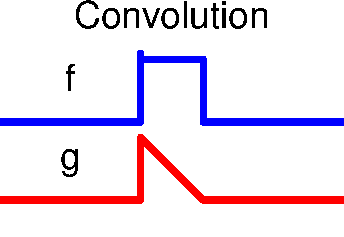
\includegraphics[page=1, width=\linewidth]{media/convolution1.pdf}
        \end{minipage}
        \hspace{.04\linewidth}
        \begin{minipage}[H]{.3\linewidth}
            \centering
            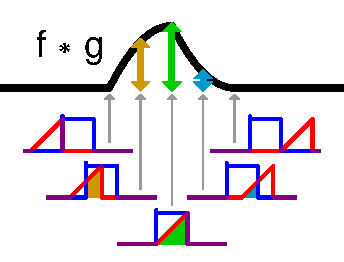
\includegraphics[page=1, width=\linewidth]{media/convolution2.pdf}
        \end{minipage}
        \caption{Esempio di una convoluzione di due funzioni \parenciteit{}{Convolution:Image}}
        \label{fig:ConvolutionExample}
    \end{figure} 
    \noindent La caratteristica \`{e} molto utile quando i calcoli differenziali si iniziano a complicare. Per capire meglio e sviluppare il discorso anche in direzione del collegamento con la fisica, proviamo a risolvere nella seguente Sezione un esempio che si collega all'elettrotecnica.
    
    \subsubsection{Elettrotecnica \& Calcolo differenziale \& Laplace} \label{sec:ElectronicsCalculusLaplace}
    Poniamo il circuito nella seguente Figura \ref{fig:CapTrasferFunctionExampleSchematic}:
    \begin{figure}[H]
        \centering
        \begin{tikzpicture}[transform shape, use fpu reciprocal]
            \draw (0,-2)
                to[sV=$U$, l_=$V_1$] ++(0,2)
                -- ++(.5,0)
                to[nopb=$SW_1$] ++(2,0)
                to[R, l=$R_1$] ++(2,0)
                -- ++(.5,0)
                to[C, l=$C_1$] ++(0,-2)
                -- ++(-5,0);
        \end{tikzpicture}
        \caption{Il circuito composto da una sorgente di tensione alternata $V_1$ di $U[V]$, un condensatore $C_1$, una resistenza $R_1$ e un interruttore $SW_1$}
        \label{fig:CapTrasferFunctionExampleSchematic}
    \end{figure}
    \noindent Quando l'interruttore $SW_1$ viene premuto, chiude il circuito e permette alla corrente di fluire dalla sorgente $U_1$ attrverso il condensatore $C_1$ e la resistenza $R_1$.

    \noindent Proviamo a descrivere la situazione dal punto di vista fisico per trovare la corrente $I$ del circuito per via del calcolo differenziale:
    \begin{figure}[H]
        \centering
        \begin{minipage}[b]{.21\linewidth}
            \centering
            \begin{equation} \label{eqn:CapTrasferFunctionExample1}
                U = A \cdot e^{j \left( \omega t + \phi \right)}
            \end{equation}
        \end{minipage}
        \hspace{0.04\linewidth}
        \begin{minipage}[b]{.21\linewidth}
            \centering
            \begin{equation} \label{eqn:CapTrasferFunctionExample2}
                \phi = 0
            \end{equation}
        \end{minipage}
        \hspace{0.04\linewidth}
        \begin{minipage}[b]{.21\linewidth}
            \centering
            \begin{equation} \label{eqn:CapTrasferFunctionExample3}
                Q = C \cdot U
            \end{equation}
        \end{minipage}
        \hspace{0.04\linewidth}
        \begin{minipage}[b]{.21\linewidth}
            \centering
            \begin{equation} \label{eqn:CapTrasferFunctionExample4}
                I = \frac{\textrm{d}Q}{\textrm{d}t}
            \end{equation}
        \end{minipage}
    \end{figure}

    \noindent Dunque:
    \begin{itemize}
        \item (\ref{eqn:CapTrasferFunctionExample1}), ci da la funzione della tensione che segue la sorgente $V_1$, che \`{e} un 
        fasore col modulo allungato di $A$ volte \emph{(l'ampiezza)}, di frequenza $\omega$, con lo sfasamento $\phi$.
        \item (\ref{eqn:CapTrasferFunctionExample2}), ci da l'informazione che la fase della funzione d'onda della sorgente non ci importa perch\`{e} se variamo lo sfasamento, lo possiamo compensare col tempo $t$ \emph{(Noi invece alla fine vedremo che troveremo una funzione che non dipende dal tempo)}.
        \item (\ref{eqn:CapTrasferFunctionExample3}), ci da la relazione tra carica $Q$, capacit\`{a} $C$ del condensatore e la sua tensione che corrisponde ad $U$.
        \item (\ref{eqn:CapTrasferFunctionExample4}), ci da un altro metodo di scrittura della corrente $I$ del circuito.
    \end{itemize} 
    \begin{align}
        I &= C \cdot \frac{\textrm{d}U}{\textrm{d}t} \label{eqn:CapTrasferFunctionExample5} \\
        I &= C \cdot \frac{\textrm{d}e^{j \left( \omega t + \phi \right)}}{\textrm{d}t} \label{eqn:CapTrasferFunctionExample6} \\
        I &= C \cdot \frac{\textrm{d}e^{j \left( \omega t\right)}}{\textrm{d}t} \label{eqn:CapTrasferFunctionExample7} \\
        I &= C \cdot e^{j \left( \omega t \right)} \cdot j \omega \label{eqn:CapTrasferFunctionExample8} \\
        I &= C U j \omega \label{eqn:CapTrasferFunctionExample9}
    \end{align}
    \begin{itemize}
        \item (\ref{eqn:CapTrasferFunctionExample5}), sostituiamo l'equazione (\ref{eqn:CapTrasferFunctionExample3}) nella carica $Q$ dell'equazione (\ref{eqn:CapTrasferFunctionExample4}).
        \item (\ref{eqn:CapTrasferFunctionExample6}), mettiamo al posto dell'$U$ l'equivalenza definita in (\ref{eqn:CapTrasferFunctionExample1}).
        \item (\ref{eqn:CapTrasferFunctionExample7}), sostituiamo lo sfasamento $\phi$ con il suo valore definito in (\ref{eqn:CapTrasferFunctionExample2}).
        \item (\ref{eqn:CapTrasferFunctionExample8}), viene ottenuta con la semplificazione della derivata su tempo $t$.
        \item (\ref{eqn:CapTrasferFunctionExample9}), la funzione d'onda viene semplificata con la $U$ per la relazione data in (\ref{eqn:CapTrasferFunctionExample1})\footnote{Occorre notare che la variabile $t$ scompare del tutto}.
    \end{itemize}

    \noindent A questo punto possiamo provare a trovare la "resistenza totale", o se detto in maniera corretta l'impedenza totale $Z$\footnote{$Z$, l'impedenza \`{e} la stessa resistenza $R$ (anche quella si misura in $[\Omega]$), che si usa quando si vuole indicare una resistenza con un valore complesso (verr\`{a} chiarito in seguito in questa Sezione)} del circuito:
    \begin{figure}[H]
        \centering
        \begin{minipage}[b]{.21\linewidth}
            \centering
            \begin{equation} \label{eqn:CapTrasferFunctionExample10}
                U = I \cdot Z
            \end{equation}
        \end{minipage}
        \hspace{0.04\linewidth}
        \begin{minipage}[b]{.21\linewidth}
            \centering
            \begin{equation} \label{eqn:CapTrasferFunctionExample11}
                I = C U j \omega
            \end{equation}
        \end{minipage}
        \hspace{0.04\linewidth}
        \begin{minipage}[b]{.21\linewidth}
            \centering
            \begin{equation} \label{eqn:CapTrasferFunctionExample12}
                s = j\omega + \sigma
            \end{equation}
        \end{minipage}
        \hspace{0.04\linewidth}
        \begin{minipage}[b]{.21\linewidth}
            \centering
            \begin{equation} \label{eqn:CapTrasferFunctionExample13}
                \sigma = 0
            \end{equation}
        \end{minipage}
    \end{figure}
    \begin{itemize}
        \item (\ref{eqn:CapTrasferFunctionExample10}), La legge di Ohm\footcite[]{Ohm:Wiki} con la variabile complessa dell'impedenza $Z$ al posto della resistenza reale $R$.
        \item (\ref{eqn:CapTrasferFunctionExample11}), riferimento all'equazione ottenuta nel calcolo precedente (\ref{eqn:CapTrasferFunctionExample9}).
        \item (\ref{eqn:CapTrasferFunctionExample12}), definizione dell'$s$ che viene data nella Sezione \ref{sec:MathAndPhysics}.
        \item (\ref{eqn:CapTrasferFunctionExample13}), assunzione che $\sigma$, il coefficiente di rafforzamento del segnale \`{e} pari a $0$.
    \end{itemize}
    \begin{align}
        Z &= \frac{U}{C U j \omega} \label{eqn:CapTrasferFunctionExample14} \\
        Z &= \frac{1}{C s} \label{eqn:CapTrasferFunctionExample15}
    \end{align}
    \begin{itemize}
        \item (\ref{eqn:CapTrasferFunctionExample14}), viene ottenuto per via della sostituzione dell'(\ref{eqn:CapTrasferFunctionExample11}) nell'$I$ della legge di Ohm (\ref{eqn:CapTrasferFunctionExample10}).
        \item (\ref{eqn:CapTrasferFunctionExample15}), semplificazione dell'equazione per la definizione dell's nel (\ref{eqn:CapTrasferFunctionExample12}).
    \end{itemize}
    \noindent Esattamente a questo punto nel procedimento ci accorgiamo che $Z$, \`{e} definita da una costante\footnote{Un condensatore ideale non cambia il suo valore di capacit\`{a}} $C$ e la variabile $s$.
    Di conseguenza possiamo scrivere la seguente funzione:
    \begin{equation} \label{eqn:CapTrasferFunctionExample16}
        Z(s) = \frac{1}{C s}
    \end{equation}

    \noindent La caratteristica di $Z(s)$ di essere una funzione con le immagini complesse, ci permette separare i valori delle impedenze in parti delle resistenze "classiche" della corrente continua, attraverso le componenti reali, e le resistenze della corrente alternata, attraverso le componenti immaginarie.

    Il calcolo differenziale che abbiamo appena risolto per trovare $Z(s)$ si pu\`{o} fare per anche altri componenti passivi\footnote{I componenti passivi si ritengono gli elementi resistenze $R$, induttanze $L$, condensatori $C$} per ottenere:
    \begin{figure}[H]
        \centering
        \begin{minipage}[b]{.3\linewidth}
            \centering
            \begin{equation*}
                Z_R(s)=R
            \end{equation*}
        \end{minipage}
        \hspace{0.04\linewidth}
        \begin{minipage}[b]{.3\linewidth}
            \centering
            \begin{equation*}
                Z_C(s) = \frac{1}{C s}
            \end{equation*}
        \end{minipage}
        \hspace*{0.04\linewidth}
        \begin{minipage}[b]{.3\linewidth}
            \centering
            \begin{equation*}
                Z_L(s) = {L s}
            \end{equation*}
        \end{minipage}
    \end{figure}
    
    Anche a livello intuitivo si pu\`{o} capire che la funzione della impedenza del condensatore mi da dei valori sempre pi\`{u} piccoli con l'aumento della frequenza.
    Questa caratteristica del condensatore potrebbe indurre il pensiero di utilizzare questa propriet\`{a} a nostro favore, ovvero per attenuare delle prime frequenze di pi\`{u} a confronto a delle seconde.
    In tale modo ci portiamo alla comprensione del concetto del funzionamento dei filtri di frequenza analogici.

    Mi permetto di modificare leggermente i nomi delle variabili e il circuito per convertirlo in un vero filtro di frequenza:
    \begin{figure}[H]
        \centering
        \begin{tikzpicture}[transform shape, use fpu reciprocal]
            \draw (0,0)
                node[left]{$U_{in}$}
                to[short, o-] ++(.25,0)
                to[R, -*, l=$R_1$] ++(2,0)
                coordinate(joint)
                to[short, -o] ++(.5,0)
                node[right]{$U_{out}$}
                (joint) to[C, l=$C_1$] ++(0,-2)
                node[ground]{} ++(0,0);
        \end{tikzpicture}
        \caption{Filtro LPF \emph{(Low Pass Filter, o filtro passa-basso che svolge la funzione di attenuare le frequenze alte del segnale)} di I grado con il segnale di entrata $U_{in}$, il segnale di uscita $U_{out}$, le altre parti sono rimaste uguali alla Figura \ref{fig:CapTrasferFunctionExampleSchematic}}
        \label{fig:CapFilterExample}
    \end{figure}

    \noindent Adesso cerchiamo di dedurre la funzione di trasferimento del filtro con la funzione dell'impedenza che abbiamo appena trovato:
    \begin{figure}[H]
        \centering
        \begin{minipage}[b]{.3\linewidth}
            \centering
            \begin{equation} \label{eqn:CapTrasferFunctionExample17}
                H(s) = \frac{U_{out}}{U_{in}}
            \end{equation}
        \end{minipage}
        \hspace{0.04\linewidth}
        \begin{minipage}[b]{.3\linewidth}
            \centering
            \begin{equation} \label{eqn:CapTrasferFunctionExample18}
                Z(s) = \frac{1}{C s}
            \end{equation}
        \end{minipage}
        \hspace*{0.04\linewidth}
        \begin{minipage}[b]{.3\linewidth}
            \centering
            \begin{equation} \label{eqn:CapTrasferFunctionExample19}
                U_{out} = U_{in} \cdot \frac{Z_b}{Z_a + Z_b}
            \end{equation}
        \end{minipage}
    \end{figure}
    \begin{itemize}
        \item (\ref{eqn:CapTrasferFunctionExample17}), uno dei modi per definire una funzione di trasferimento menzionato nella Sezione \ref{sec:MathAndPhysics}.
        \item (\ref{eqn:CapTrasferFunctionExample18}), funzione dell'impedenza del condensatore appena calcolata (\ref{eqn:CapTrasferFunctionExample16}).
        \item (\ref{eqn:CapTrasferFunctionExample19}), formula che provviene dalle leggi di Ohm e Kirchhoff\footcite[]{Kirchhoff:Wiki} che ci permette di calcolare la tensione nel punto $U_{out}$ sapendo il valore delle resistenze e la tensione di entrata $U_{in}$.
    \end{itemize}
    \begin{align}
        U_{out} &= U_{in} \cdot \frac{\frac{1}{C s}}{\frac{1}{C s}+R} \label{eqn:CapTrasferFunctionExample20} \\
        \frac{U_{out}}{U_{in}} &= \frac{\frac{1}{C s}}{\frac{1}{C s}+R} \label{eqn:CapTrasferFunctionExample21} \\
        H(s) &= \frac{\frac{1}{C s}}{\frac{1}{C s}+R} \label{eqn:CapTrasferFunctionExample22} \\
        H(s) &= \frac{1}{R C s + 1} \label{eqn:CapTrasferFunctionExample23}
    \end{align}
    \begin{itemize}
        \item (\ref{eqn:CapTrasferFunctionExample20}), sostituzione dei valori di $R_1$ e $C_1$ \emph{(l'impedenza $Z$ (\ref{eqn:CapTrasferFunctionExample18}))} nel (\ref{eqn:CapTrasferFunctionExample19}) \emph{(ovviamente sostituendo i i nomi della prima impedenza $Z_a$ con $R$ e la seconda $Z_b$ con $Z(s)$)}.
        \item (\ref{eqn:CapTrasferFunctionExample21}), divisione da due parti dell'equazione per $U_{in}$.
        \item (\ref{eqn:CapTrasferFunctionExample22}), sostituzione dell'$\frac{U_{out}}{U_{in}}$ con (\ref{eqn:CapTrasferFunctionExample17}).
        \item (\ref{eqn:CapTrasferFunctionExample23}), moltiplicazione per $C s$ al numeratore e al denominatore della frazione.
    \end{itemize}
    \noindent La funzione che abbiamo trovato ha la caratteristica forma della funzione di trasferimento gi\`{a} vista nella Sezione \ref{sec:TransformsAndLaplace}, che in questo caso \`{e} solamente di I grado.
    Inoltre vale il fatto che ho gi\`{a} riportato precedentemente\footnote{Sezione \ref{sec:TransformsAndLaplace}}: i calcoli sono abbastanza numerosi per un circuito davvero semplice. 
    Ecco il momento dove viene d'aiuto\footnote{Il suo maggiore potenziale si fa vedere quando i circuiti diventano delle reti di componenti passivi che sono molto difficili da descrivere col calcolo differenziale e in seguito semplificarli per renderli adoperabili} la trasformata di Laplace.

    \noindent Proviamo a complicare il filtro cancatenandoci delle sue copie all'input:
    \begin{figure}[H]
        \centering
        \begin{tikzpicture}[transform shape, use fpu reciprocal]
            \draw (0,0)
                node[left]{$U_{in}$}
                to[short, o-] ++(.25,0)
                to[R, -*, l=$R_1$] ++(2,0)
                coordinate(joint)
                to[C, l=$C_1$] ++(0,-2)
                node[ground]{} ++(0,-.15)
                (joint) to[R, -*, l=$R_2$] ++(2,0)
                coordinate(joint1)
                to[C, l=$C_2$] ++(0,-2)
                node[ground]{} ++(0,-.15)
                (joint1) to[R, -*, l=$R_3$] ++(2,0)
                coordinate(joint2)
                to[C, l=$C_3$] ++(0,-2)
                node[ground]{} ++(0,0)
                (joint2) to[short, -o] ++(.5,0)
                node[right]{$U_{out}$};
        \end{tikzpicture}
        \caption{Filtro LPF di III grado con il segnale di entrata $U_{in}$, il segnale di uscita $U_{out}$, con i componenti passivi \emph{($R_x$, $C_x$)} ottenuti dalla concatenazione delle copie del filtro in Figura \ref{fig:CapFilterExample}}
        \label{fig:CapFilterExample2}
    \end{figure}
    \noindent In questo esempio poniamo che per avere fatto delle copie del filtro dell'esempio precedente\footnote{\ref{fig:CapFilterExample}} la seguente condizione:
    \begin{figure}[H]
        \centering
        \begin{minipage}[b]{.31\linewidth}
            \centering
            \begin{equation*}
                R = R_1 = R_2 = R_3
            \end{equation*}
        \end{minipage}
        \hspace{0.04\linewidth}
        \begin{minipage}[b]{.31\linewidth}
            \centering
            \begin{equation*}
                C = C_1 = C_2 = C_3
            \end{equation*}
        \end{minipage}
    \end{figure}
    \noindent Per trovare la risposta del sistema $U_{out}$ a un segnale $U_{in}$ al posto di descrivere il circuito con il calcolo differenziale basta comporre la seguente espressione:
    \begin{equation*}
        H_{LPF\_III}(s) = \frac{1}{RCs+1} \cdot \frac{1}{RCs+1} \cdot \frac{1}{RCs+1} = \frac{1}{\left(RCs+1\right)^3}
    \end{equation*}
    \noindent In seguito si prende la trasformata inversa di Laplace della funzione di trasferimento appena ottenuta:
    \begin{equation*}
        \mathcal{L}^{-1}\{H_{LPF\_III}\}(t) = \int_{c-j\infty}^{c+j\infty} e^{f_{LPF\_III}t} H_{LPF\_III}(s) \mathrm{d}s
    \end{equation*}
    \noindent La trasformata inversa \`{e} pi\`{u} difficile dal punto di vista del calcolo della trasformata stessa, ma esistono le tavole delle espressioni gi\`{a} calcolate di concetto simili alle regole della derivazione.
    Inoltre, per comodit\`{a} e per evitare di commettere errori utilizzo una lingua di programmaggio chiamata Maple\footcite[]{Maplesoft:Software} che possiede la possibilit\`{a} di adoperare espressioni matematiche in forma algebrica\footnote{Python, R, Matlab, delle lignue di programmaggio molto conosciute per la loro comodit\`{a} d'uso per calcoli matematici, che purtroppo non riescono ad adoperare i calcoli con dei parametri non dichiarati} e che ha uso di un Software per comodit\`{a}.
    Dunque, attraverso Maple otteniamo:
    \begin{equation*}
        \mathcal{L}^{-1}\{H_{LPF\_III}\}(t) = f_{LPF\_III}(t) = t^2 \cdot \frac{e^{-\frac{t}{RC}}}{2RC^3}
    \end{equation*}
    Come verifica di correttezza del risultato ottenuto, possiamo notare che la funzione \`{e} una funzione armonica.

    A questo punto possiamo transitare il discorso dalle trasformate di Laplace nella direzione dell'elettrotecnica con le conoscenze a disposizione.

    \subsubsection{Tipi di filtri di frequenza}
    Per lavorare con le funzioni di trasferimento nel dominio delle frequenze dal punto di vista grafico dobbiamo prima convertirle in un determinato modo perch\'{e} inizialmente le immagini sono dei numeri complessi.
    Per ottenere il fattore di quanto le funzioni di trasferimento amplificano il segnale dobbiamo prendere il modulo della funzione di trasferimento, mentre per ottenere lo sfasamento occorre prendere l'argomento della funzione:
    \begin{figure}[H]
        \centering
        \begin{minipage}[b]{.31\linewidth}
            \centering
            \begin{equation*}
                A = \left|H(s)\right|
            \end{equation*}
        \end{minipage}
        \hspace{0.04\linewidth}
        \begin{minipage}[b]{.31\linewidth}
            \centering
            \begin{equation*}
                \theta = \angle\left(H(s)\right)
            \end{equation*}
        \end{minipage}
    \end{figure}
    \noindent Sapendo questo possiamo studiarle.

    Per semplificare i concetti suddivido le funzioni di trasferimento dei filtri in semplici e complicate: le semplici sono le funzioni di trasferimento che si possono combinare in modi diversi per variare la funzione complicata che si ottiene.
    
    \noindent Scopra i grafici seguenti \ref{fig:SimpleBodeExample} e \ref{fig:ComplicateBodeExample}:
    \begin{figure}[H]
        \centering
        \begin{minipage}[H]{.45\linewidth}
            \centering
            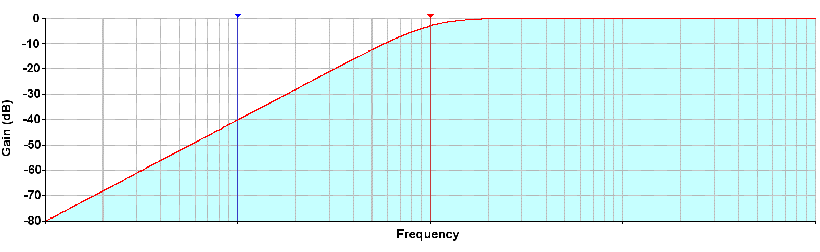
\includegraphics[width=\linewidth]{media/sloa093_HPF.pdf}
            \subcaption{}
            \label{fig:SimpleBodeExampleHPF}
        \end{minipage}
        \hspace{.04\linewidth}
        \begin{minipage}[H]{.45\linewidth}
            \centering
            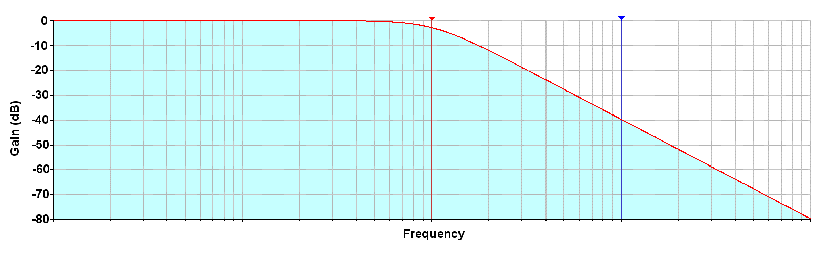
\includegraphics[width=\linewidth]{media/sloa093_LPF.pdf}
            \subcaption{}
            \label{fig:SimpleBodeExampleLPF}
        \end{minipage}
        \caption{Esempio di risposta dell'amplificazione nel dominio della frequenza delle funzioni di trasferimento semplici: \ref{fig:SimpleBodeExampleHPF} High-Pass o HPF, passa-alto che attenua le frequenze basse, \ref{fig:SimpleBodeExampleLPF} Low-Pass o LPF, passa-basso che attenua le frequenze alte \emph{(l'"F" delle abbreviazioni indica la parola Filter o filtro) \parenciteit{}{FilterPassStopTypes:Image}}}
        \label{fig:SimpleBodeExample}
    \end{figure}
    \noindent Le funzioni complicate invece sono:
    \begin{figure}[H]
        \centering
        \begin{minipage}[H]{.45\linewidth}
            \centering
            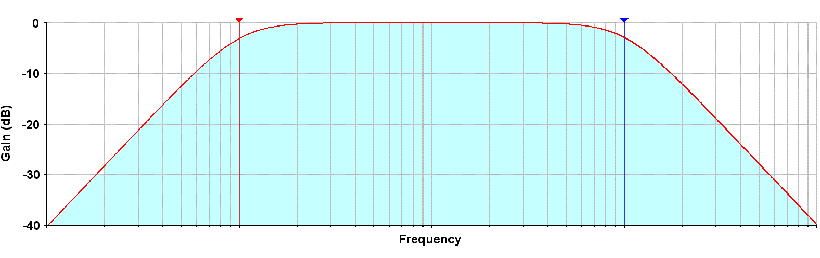
\includegraphics[width=\linewidth]{media/sloa093_BPF.pdf}
            \subcaption{}
            \label{fig:ComplicateBodeExampleBPF}
        \end{minipage}
        \hspace{.04\linewidth}
        \begin{minipage}[H]{.45\linewidth}
            \centering
            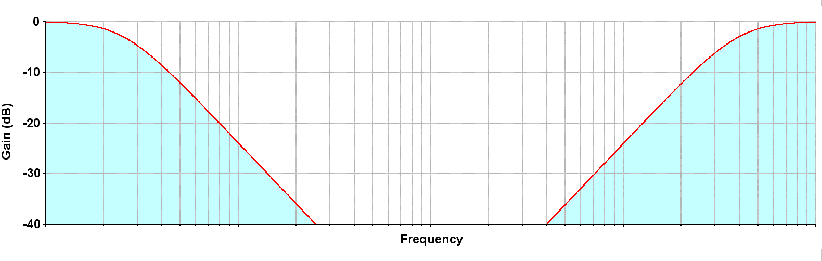
\includegraphics[width=\linewidth]{media/sloa093_BSF.pdf}
            \subcaption{}
            \label{fig:ComplicateBodeExampleBSF}
        \end{minipage}
        \\
        \begin{minipage}[H]{.45\linewidth}
            \centering
            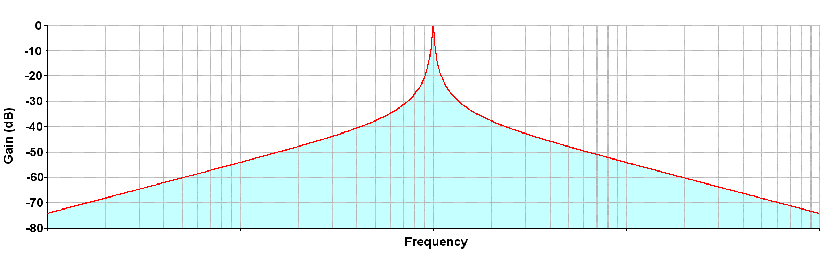
\includegraphics[width=\linewidth]{media/sloa093_NPF.pdf}
            \subcaption{}
            \label{fig:ComplicateBodeExampleNPF}
        \end{minipage}
        \hspace{.04\linewidth}
        \begin{minipage}[H]{.45\linewidth}
            \centering
            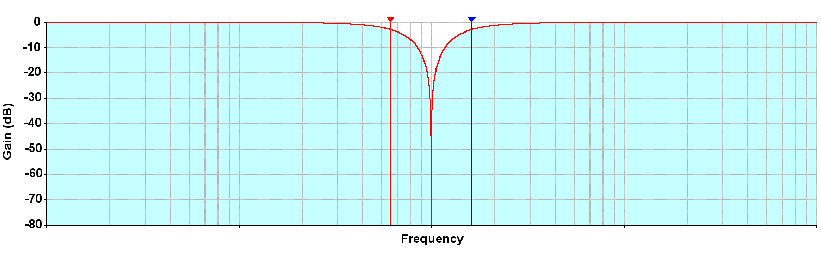
\includegraphics[width=\linewidth]{media/sloa093_NSF.pdf}
            \subcaption{}
            \label{fig:ComplicateBodeExampleNSF}
        \end{minipage}
        \caption{Esempio di risposta dell'amplificazione nel dominio della frequenza delle funzioni di trasferimento complicate: \ref{fig:ComplicateBodeExampleBPF} Band-Pass o BPF, passa-banda che fa passare una banda di frequenze, \ref{fig:ComplicateBodeExampleBSF} Band-Rejection o BRF, ferma-banda che attenua una banda di frequenze, \ref{fig:ComplicateBodeExampleNPF} Narrow-Band-Pass o NPF, passa-banda sottile che fa passare una sottile banda di frequenze, \ref{fig:ComplicateBodeExampleNSF} Narrow-Band-Rejection o NRF, ferma-banda sottile che attenua una sottile banda di frequenze \parenciteit{}{FilterPassStopTypes:Image}}
        \label{fig:ComplicateBodeExample}
    \end{figure}
    \clearpage

    \noindent La variazione dell'ordine del filtro e del parametro $\sigma$ nel dominio delle frequenze si manifestano nel seguente modo, come nella Figura \ref{fig:FunctionShapesOrder}:
    \begin{figure}[H]
        \centering
        \begin{minipage}[H]{.45\linewidth}
            \centering
            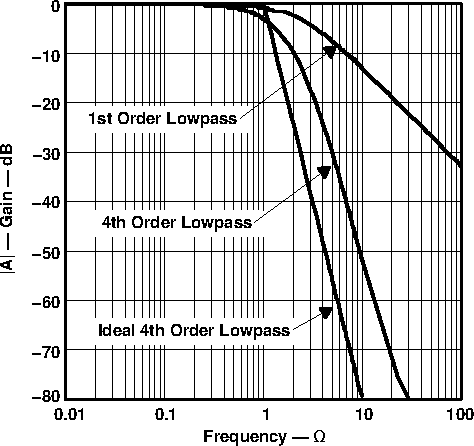
\includegraphics[width=\linewidth]{media/sloa088_order.pdf}
            \label{fig:FunctionOrder}
            \subcaption{Le funzioni di trasferimento di forma  di diversa forma che viene data dalla variazione del loro ordine}
        \end{minipage}
        \hspace{.04\linewidth}
        \begin{minipage}[H]{.45\linewidth}
            \centering
            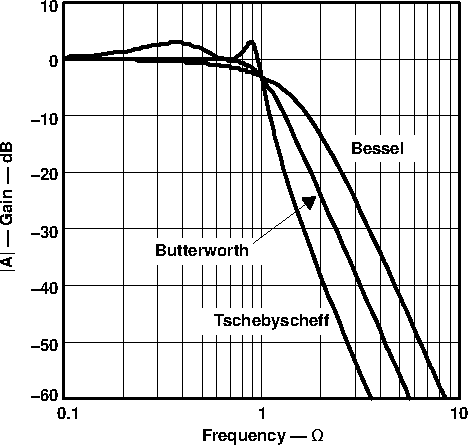
\includegraphics[width=\linewidth]{media/sloa088_shape.pdf}
            \label{fig:FunctionShapes}
            \subcaption{Le funzioni di trasferimento di diversa forma che viene data dalla variazione della $\sigma$}
        \end{minipage}
        \caption{Esempio di risposta dell'amplificazione nel dominio della frequenza delle funzioni normalizzate \emph{(Con $\Omega$ si indica che la frequenza normalizzata, ovvero la frequenza cutoff o di taglio della funzione \`{e} stata spostata al valore $1$)} di trasferimento passa-basso \parenciteit{}{SLOA088}}
        \label{fig:FunctionShapesOrder}
    \end{figure}
    \noindent L'ordine del filtro analogico si pu\`{o} variare solo aggiungendo componenti nella rete\footnote{Si pu\`{o} dedurre dalle conoscenze date nella Sezione \ref{sec:ElectronicsCalculusLaplace}} di impedenze, per il fatto che un elemento elettrotecnico passivo pu\`{o} al massimo contenerne una.
    La forma della funzione invece \`{e} un compromesso della velocit\`{a} di taglio delle frequenze e il quanto piatta \`{e} la risposta della parte della funzione che deve rimanere intatta.

    Nel mio progetto, lo sfasamento della funzione di trasferimento risulta indifferente\footnote{Ritengo che l'intelligenza artificiale che dovr\`{a} elaborare le informazioni ricevute nelle future iterazioni del progetto, non \`{e} influenzata dallo sfasamento del segnale: basta che sia una funzione identica in tutte le schede sensore}, per questo mi permetto di saltare la parte della descrizione delle caratteristiche delle diverse forme della funzione.
    Presento invece una singola forma: Butterworth\footnote{Viene dimostrata nella Figura \ref{fig:FunctionShapesOrder}}, la pi\`{u} efficace dal punto di vista del quanto \`{e} piatta la parte della funzione che deve rimanere intatta e quanto veloce viene tagliata alla frequenza necessaria\footnote{Concetto preso dalla spiegazione di \parenciteit{p6}{SLOA088}}.
    Butterworth, ha la velocit\`{a} di taglio\footnote{Detta anche rolloff rate} di 20dB/dec\footnote{L'unit\`{a} di misura indica di quanto diminuisce l'amplificazione del filtro dopo il cambio della frequenza di un fattore di dieci} per ordine\footnote{La velocit\`{a} del taglio di un determinato ordine si pu\`{o} trovare moltiplicando l'ordine del filtro per la velocit\`{a} del taglio di ordine I}.

    Per vedere meglio come si formano le funzioni di trasferimento variando il parametro $\sigma$, ho deciso di metterlo su uno degli assi delle coordinate ed ho ottenuto i seguenti grafici nella Figura \ref{fig:3DFUNCExample}:
    \begin{figure}[H]
        \centering
        \begin{minipage}[H]{.45\linewidth}
            \centering
            \newcommand{\plotDir}{datasets/s_plot_example_data}
            \newcommand{\plotName}{hpf_2}
            \import{\plotDir}{\plotName_def.tex}%
            \begin{tikzpicture}
                \begin{axis}[
                    width=\linewidth,
                    view = {20}{30},
                    % ymode=log,
                    xmin = \minX,
                    xmax = \maxX,
                    ymin = \minY,
                    ymax = \maxY,
                    zmin = \minZ,
                    zmax = \maxZ,
                    xtick = {\minTickX,\nextTickX,...,\maxTickX},
                    ytick = {\minTickY,\nextTickY,...,\maxTickY},
                    ztick = {\minTickZ,\nextTickZ,...,\maxTickZ},
                    xlabel={\legendX},
                    ylabel={\legendY},
                    zlabel={\legendZ},
                    label style={font=\footnotesize},
                    tick label style={font=\tiny},
                    smooth,
                    grid = both,
                    ymajorgrids = true,
                    line join=round,
                    clip=false
                ]
                \addplot3[
                    surf,
                    /pgfplots/colormap={bone}{rgb255=(0,0,0) rgb255=(84,84,116) rgb255=(167,199,199) rgb255=(240,240,240)},
                    opacity=0.9375,
                    shader=faceted interp,
                    patch type=coons,
                    z buffer=sort,
                    patch table=\plotDir/\plotName_anchors.csv
                ] table [col sep=comma,header=false] {\plotDir/\plotName.csv};
                \end{axis}
            \end{tikzpicture}
            \import{\plotDir}{All_plots_undef.tex}%
            \let\plotDir\undefined
            \let\plotName\undefined
            \subcaption{}
            \label{fig:HPF2Example}
        \end{minipage}
        \hspace{.04\linewidth}
        \begin{minipage}[H]{.45\linewidth}
            \centering
            \newcommand{\plotDir}{datasets/s_plot_example_data}
            \newcommand{\plotName}{lpf_2}
            \import{\plotDir}{\plotName_def.tex}%
            \begin{tikzpicture}
                \begin{axis}[
                    width=\linewidth,
                    view = {20}{30},
                    % ymode=log,
                    xmin = \minX,
                    xmax = \maxX,
                    ymin = \minY,
                    ymax = \maxY,
                    zmin = \minZ,
                    zmax = \maxZ,
                    xtick = {\minTickX,\nextTickX,...,\maxTickX},
                    ytick = {\minTickY,\nextTickY,...,\maxTickY},
                    ztick = {\minTickZ,\nextTickZ,...,\maxTickZ},
                    xlabel={\legendX},
                    ylabel={\legendY},
                    zlabel={\legendZ},
                    label style={font=\footnotesize},
                    tick label style={font=\tiny},
                    smooth,
                    grid = both,
                    ymajorgrids = true,
                    line join=round,
                    clip=false
                ]
                \addplot3[
                    surf,
                    /pgfplots/colormap={bone}{rgb255=(0,0,0) rgb255=(84,84,116) rgb255=(167,199,199) rgb255=(240,240,240)},
                    opacity=0.9375,
                    shader=faceted interp,
                    patch type=coons,
                    z buffer=sort,
                    patch table=\plotDir/\plotName_anchors.csv
                ] table [col sep=comma,header=false] {\plotDir/\plotName.csv};
                \end{axis}
            \end{tikzpicture}
            \import{\plotDir}{All_plots_undef.tex}%
            \let\plotDir\undefined
            \let\plotName\undefined
            \subcaption{}
            \label{fig:LPF2Example}
        \end{minipage}
        \\
        \begin{minipage}[H]{.45\linewidth}
            \centering
            \newcommand{\plotDir}{datasets/s_plot_example_data}
            \newcommand{\plotName}{bpf_2}
            \import{\plotDir}{\plotName_def.tex}%
            \begin{tikzpicture}
                \begin{axis}[
                    width=\linewidth,
                    view = {20}{30},
                    % ymode=log,
                    xmin = \minX,
                    xmax = \maxX,
                    ymin = \minY,
                    ymax = \maxY,
                    zmin = \minZ,
                    zmax = \maxZ,
                    xtick = {\minTickX,\nextTickX,...,\maxTickX},
                    ytick = {\minTickY,\nextTickY,...,\maxTickY},
                    ztick = {\minTickZ,\nextTickZ,...,\maxTickZ},
                    xlabel={\legendX},
                    ylabel={\legendY},
                    zlabel={\legendZ},
                    label style={font=\footnotesize},
                    tick label style={font=\tiny},
                    smooth,
                    grid = both,
                    ymajorgrids = true,
                    line join=round,
                    clip=false
                ]
                \addplot3[
                    surf,
                    /pgfplots/colormap={bone}{rgb255=(0,0,0) rgb255=(84,84,116) rgb255=(167,199,199) rgb255=(240,240,240)},
                    opacity=0.9375,
                    shader=faceted interp,
                    patch type=coons,
                    z buffer=sort,
                    patch table=\plotDir/\plotName_anchors.csv
                ] table [col sep=comma,header=false] {\plotDir/\plotName.csv};
                \end{axis}
            \end{tikzpicture}
            \import{\plotDir}{All_plots_undef.tex}%
            \let\plotDir\undefined
            \let\plotName\undefined
            \subcaption{}
            \label{fig:BPF2Example}
        \end{minipage}
        \hspace{.04\linewidth}
        \begin{minipage}[H]{.45\linewidth}
            \centering
            \newcommand{\plotDir}{datasets/s_plot_example_data}
            \newcommand{\plotName}{bpf_4}
            \import{\plotDir}{\plotName_def.tex}%
            \begin{tikzpicture}
                \begin{axis}[
                    width=\linewidth,
                    view = {20}{30},
                    % ymode=log,
                    xmin = \minX,
                    xmax = \maxX,
                    ymin = \minY,
                    ymax = \maxY,
                    zmin = \minZ,
                    zmax = \maxZ,
                    xtick = {\minTickX,\nextTickX,...,\maxTickX},
                    ytick = {\minTickY,\nextTickY,...,\maxTickY},
                    ztick = {\minTickZ,\nextTickZ,...,\maxTickZ},
                    xlabel={\legendX},
                    ylabel={\legendY},
                    zlabel={\legendZ},
                    label style={font=\footnotesize},
                    tick label style={font=\tiny},
                    smooth,
                    grid = both,
                    ymajorgrids = true,
                    line join=round,
                    clip=false
                ]
                \addplot3[
                    surf,
                    /pgfplots/colormap={bone}{rgb255=(0,0,0) rgb255=(84,84,116) rgb255=(167,199,199) rgb255=(240,240,240)},
                    opacity=0.9375,
                    shader=faceted interp,
                    patch type=coons,
                    z buffer=sort,
                    patch table=\plotDir/\plotName_anchors.csv
                ] table [col sep=comma,header=false] {\plotDir/\plotName.csv};
                \end{axis}
            \end{tikzpicture}
            \import{\plotDir}{All_plots_undef.tex}%
            \let\plotDir\undefined
            \let\plotName\undefined
            \subcaption{}
            \label{fig:BPF4Example}
        \end{minipage}
        \begin{minipage}[H]{.45\linewidth}
            \centering
            \newcommand{\plotDir}{datasets/s_plot_log_example_data}
            \newcommand{\plotName}{hpf_2}
            \import{\plotDir}{\plotName_def.tex}%
            \begin{tikzpicture}
                \begin{axis}[
                    width=\linewidth,
                    view = {70}{30},
                    ymode=log,
                    log ticks with fixed point,
                    xmin = \minX,
                    xmax = \maxX,
                    ymin = \minY,
                    ymax = \maxY,
                    zmin = \minZ,
                    zmax = \maxZ,
                    xtick = {\minTickX,\nextTickX,...,\maxTickX},
                    ytick = {\minTickY,\nextTickY,...,\maxTickY},
                    ztick = {\minTickZ,\nextTickZ,...,\maxTickZ},
                    xlabel={\legendX},
                    ylabel={\legendY},
                    zlabel={\legendZ},
                    label style={font=\footnotesize},
                    tick label style={font=\tiny},
                    smooth,
                    grid = both,
                    ymajorgrids = true,
                    line join=round,
                    clip=false,
                    y tick label style = {rotate=-60, anchor=west}
                ]
                \addplot3[
                    surf,
                    /pgfplots/colormap={bone}{rgb255=(0,0,0) rgb255=(84,84,116) rgb255=(167,199,199) rgb255=(240,240,240)},
                    opacity=0.9375,
                    shader=faceted interp,
                    patch type=coons,
                    z buffer=sort,
                    patch table=\plotDir/\plotName_anchors.csv
                ] table [col sep=comma,header=false] {\plotDir/\plotName.csv};
                \end{axis}
            \end{tikzpicture}
            \import{\plotDir}{All_plots_undef.tex}%
            \let\plotDir\undefined
            \let\plotName\undefined
            \subcaption{}
            \label{fig:HPF2logExample}
        \end{minipage}
        \hspace{.04\linewidth}
        \begin{minipage}[H]{.45\linewidth}
            \centering
            \newcommand{\plotDir}{datasets/s_plot_log_example_data}
            \newcommand{\plotName}{lpf_2}
            \import{\plotDir}{\plotName_def.tex}%
            \begin{tikzpicture}
                \begin{axis}[
                    width=\linewidth,
                    view = {70}{30},
                    ymode=log,
                    log ticks with fixed point,
                    xmin = \minX,
                    xmax = \maxX,
                    ymin = \minY,
                    ymax = \maxY,
                    zmin = \minZ,
                    zmax = \maxZ,
                    xtick = {\minTickX,\nextTickX,...,\maxTickX},
                    ytick = {\minTickY,\nextTickY,...,\maxTickY},
                    ztick = {\minTickZ,\nextTickZ,...,\maxTickZ},
                    xlabel={\legendX},
                    ylabel={\legendY},
                    zlabel={\legendZ},
                    label style={font=\footnotesize},
                    tick label style={font=\tiny},
                    smooth,
                    grid = both,
                    ymajorgrids = true,
                    line join=round,
                    clip=false,
                    y tick label style = {rotate=-60, anchor=west}
                ]
                \addplot3[
                    surf,
                    /pgfplots/colormap={bone}{rgb255=(0,0,0) rgb255=(84,84,116) rgb255=(167,199,199) rgb255=(240,240,240)},
                    opacity=0.9375,
                    shader=faceted interp,
                    patch type=coons,
                    z buffer=sort,
                    patch table=\plotDir/\plotName_anchors.csv
                ] table [col sep=comma,header=false] {\plotDir/\plotName.csv};
                \end{axis}
            \end{tikzpicture}
            \import{\plotDir}{All_plots_undef.tex}%
            \let\plotDir\undefined
            \let\plotName\undefined
            \subcaption{}
            \label{fig:LPF2logExample}
        \end{minipage}
        \\
        \begin{minipage}[H]{.45\linewidth}
            \centering
            \newcommand{\plotDir}{datasets/s_plot_log_example_data}
            \newcommand{\plotName}{bpf_2}
            \import{\plotDir}{\plotName_def.tex}%
            \begin{tikzpicture}
                \begin{axis}[
                    width=\linewidth,
                    view = {70}{30},
                    ymode=log,
                    log ticks with fixed point,
                    xmin = \minX,
                    xmax = \maxX,
                    ymin = \minY,
                    ymax = \maxY,
                    zmin = \minZ,
                    zmax = \maxZ,
                    xtick = {\minTickX,\nextTickX,...,\maxTickX},
                    ytick = {\minTickY,\nextTickY,...,\maxTickY},
                    ztick = {\minTickZ,\nextTickZ,...,\maxTickZ},
                    xlabel={\legendX},
                    ylabel={\legendY},
                    zlabel={\legendZ},
                    label style={font=\footnotesize},
                    tick label style={font=\tiny},
                    smooth,
                    grid = both,
                    ymajorgrids = true,
                    line join=round,
                    clip=false,
                    y tick label style = {rotate=-60, anchor=west}
                ]
                \addplot3[
                    surf,
                    /pgfplots/colormap={bone}{rgb255=(0,0,0) rgb255=(84,84,116) rgb255=(167,199,199) rgb255=(240,240,240)},
                    opacity=0.9375,
                    shader=faceted interp,
                    patch type=coons,
                    z buffer=sort,
                    patch table=\plotDir/\plotName_anchors.csv
                ] table [col sep=comma,header=false] {\plotDir/\plotName.csv};
                \end{axis}
            \end{tikzpicture}
            \import{\plotDir}{All_plots_undef.tex}%
            \let\plotDir\undefined
            \let\plotName\undefined
            \subcaption{}
            \label{fig:BPF2logExample}
        \end{minipage}
        \hspace{.04\linewidth}
        \begin{minipage}[H]{.45\linewidth}
            \centering
            \newcommand{\plotDir}{datasets/s_plot_log_example_data}
            \newcommand{\plotName}{bpf_4}
            \import{\plotDir}{\plotName_def.tex}%
            \begin{tikzpicture}
                \begin{axis}[
                    width=\linewidth,
                    view = {70}{30},
                    ymode=log,
                    log ticks with fixed point,
                    xmin = \minX,
                    xmax = \maxX,
                    ymin = \minY,
                    ymax = \maxY,
                    zmin = \minZ,
                    zmax = \maxZ,
                    xtick = {\minTickX,\nextTickX,...,\maxTickX},
                    ytick = {\minTickY,\nextTickY,...,\maxTickY},
                    ztick = {\minTickZ,\nextTickZ,...,\maxTickZ},
                    xlabel={\legendX},
                    ylabel={\legendY},
                    zlabel={\legendZ},
                    label style={font=\footnotesize},
                    tick label style={font=\tiny},
                    smooth,
                    grid = both,
                    ymajorgrids = true,
                    line join=round,
                    clip=false,
                    y tick label style = {rotate=-60, anchor=west}
                ]
                \addplot3[
                    surf,
                    /pgfplots/colormap={bone}{rgb255=(0,0,0) rgb255=(84,84,116) rgb255=(167,199,199) rgb255=(240,240,240)},
                    opacity=0.9375,
                    shader=faceted interp,
                    patch type=coons,
                    z buffer=sort,
                    patch table=\plotDir/\plotName_anchors.csv
                ] table [col sep=comma,header=false] {\plotDir/\plotName.csv};
                \end{axis}
            \end{tikzpicture}
            \import{\plotDir}{All_plots_undef.tex}%
            \let\plotDir\undefined
            \let\plotName\undefined
            \subcaption{}
            \label{fig:BPF4logExample}
        \end{minipage}
        \caption{Quattro funzioni di trasferimento di tipi e ordini diversi con l'asse dell'amplificazione in scala logaritmica con l'asse delle frequenze $\omega$ in scala decimale in \ref{fig:HPF2Example} \ref{fig:LPF2Example} \ref{fig:BPF2Example} \ref{fig:BPF4Example} e in scala logaritmica \ref{fig:HPF2logExample} \ref{fig:LPF2logExample} \ref{fig:BPF2logExample} \ref{fig:BPF4logExample}}
        \label{fig:3DFUNCExample}
    \end{figure}
    \clearpage

    \subsubsection{Elettrotecnica \& Filtri}
    I filtri che abbiamo visto nella Sezione \ref{sec:ElectronicsCalculusLaplace} nelle Figure \ref{fig:CapFilterExample} e \ref{fig:CapFilterExample2} aumentano la resistenza dell'output e la lunica cosa che fanno \`{e} attenuare il segnale segnale\footnote{Nel mondo reale per leggere una tensione da un conduttore fluisce della corrente e per l'impedenza del filtro (anche per la parte delle frequenze che non devono essere attenuate) la tensione diminuisce}.
    Di conseguenza dobbiamo amplificare il segnale per aumentare l'ordine del filtro.
    La prima idea che viene \`{e} quella di mettere in serie al filtro un amplificatore operazionale o OA, ma questa scelta non \`{e} la migliore, perch\`{e} esistono direttamente dei filtri attivi, ovvero che includono nella loro topologia un amplificatore.
    Le pi\`{u} semplici e popolari sono SK o Sallen-Key e MFB o Multiple-Feedback-Filter, che si possono vedere nella seguente Figura \ref{fig:SKMFBSchematic}
    \begin{figure}[H]
        \centering
        \begin{minipage}[H]{.45\linewidth}
            \centering
            \begin{tikzpicture}[transform shape, use fpu reciprocal, scale=.75]
                \draw (0,0)
                    to[R, l=$R_1$, -*] ++(2,0)
                    coordinate(C1)
    
                    to[R, l=$R_2$, -*] ++(2,0)
                    coordinate(C2)
    
                    (C2)
                    -- ++(1.25,0)
                    node[op amp, noinv input up, fill=cyan!20, anchor=+](OA1){\texttt{OA1}}
    
                    (C2)
                    to[C, l=$C_2$] ++(0,-2)
                    node[tlground]{}
    
                    (OA1.-)
                    -- ++ (-.25,0)
                    -- ++(0,-1.75)
                    coordinate(Rg1Rg2)
                    to[R, l=$R_{G1}$, *-] (Rg1Rg2-|OA1.out)
                    to[short, -*] (OA1.out)
    
                    (Rg1Rg2) to[R, l=$R_{G2}$] ++(0,-2)
                    node[tlground]{}
    
                    (C1)
                    -- ++(0,1.5)
                    coordinate(R1start)
                    to[C, l=$C_1$] (R1start-|OA1.out)
                    -- (OA1.out)
    
                    (OA1.up)
                    node[vcc]{$V_{CC}$}
    
                    (OA1.down)
                    node[ground]{}
    
                    (OA1.out) ++(.5,0)
                    node[right]{$U_{out}$}
                    to[short, o-] ++(-.5,0)
    
                    (0,0)
                    node[left]{$U_{in}$}
                    to[short, o-] ++(0,0)
                    ;
            \end{tikzpicture}
            \subcaption{Topologia Sallen-Key, ha il lato positivo di avere i valori della $\sigma$ e dell'amplificazione indipendenti \emph{($R_{GX}$ aggiustano l'amplificazione, $RX$ e $CX$ la $\sigma$)}}
            \label{fig:SKSchematic}
        \end{minipage}
        \hspace{.04\linewidth}
        \begin{minipage}[H]{.45\linewidth}
            \centering
            \begin{tikzpicture}[transform shape, use fpu reciprocal, scale=.75]
                \draw (0,0)
                    to[R, l=$R_1$, -*] ++(2,0)
                    coordinate(C1)
    
                    to[R, l=$R_3$, -*] ++(2,0)
                    coordinate(C2)
                    -- ++(.75,0)
                    node[op amp, noinv input down, fill=cyan!20, anchor=-](OA1){\texttt{OA1}}
    
                    (OA1.+)
                    -- ++(-.25,0)
                    node[ground]{}
    
                    (OA1.up)
                    node[vcc]{$V_{CC}$}
    
                    (OA1.down)
                    node[ground]{}
    
                    (C1)
                    to[C, l=$C_1$] ++(0,-2)
                    node[tlground]{}
    
                    (C2)
                    -- ++(0,1.5)
                    coordinate(R2start)
                    to[C, l=$C_2$, -*] (R2start-|OA1.out)
                    coordinate(R2)
                    to[short, -*] (OA1.out)
    
                    (C1)
                    -- ++(0,2.5)
                    coordinate(C3start)
                    to[R, l=$R_2$] (C3start-|OA1.out)
                    -- (R2)
    
                    (OA1.out) ++(.5,0)
                    node[right]{$U_{out}$}
                    to[short, o-] ++(-.5,0)
    
                    (0,0)
                    node[left]{$U_{in}$}
                    to[short, o-] ++(0,0)
                    ;
            \end{tikzpicture}
            \subcaption{Topologia Multiple-Feedback, ha il lato positivo di avere meno componenti passivi ed essere meno sensibile al cambio dei loro valori \emph{(I componenti passivi hanno i loro valori non totalmente costanti, prevalentemente dipendono dalla temperatura dell'ambiente nel quale si trovano)} e la caratteristica di invertire il segnale}
            \label{fig:MFBSchematic}
        \end{minipage}
        \hspace{.04\linewidth}
        \caption{Diagramma di due circuiti LPF attivi di II ordine}
        \label{fig:SKMFBSchematic}
    \end{figure}


    \noindent Per calcolare la funzione di trasferimento di questi filtri ho applicato la seguente tecnica:
    \begin{enumerate}[label=\emph{(\roman*)}]
        \item Utilizzare le funzioni ricavate dalla trasformata di Laplace per i componenti passivi.
        \item Utilizzare le leggi di Ohm e leggi di Kirchhoff per comporre le equazioni del circuito, ovvero le relazioni tra le correnti differenti che sono presenti nel circuito
        \item Comporre un sistema di equazioni che descrive le relazioni tra le differenti correnti definite in forma $I=\frac{U}{Z(s)}$
        \item Eliminare tutte le correnti tranne $\frac{U_{out}}{U_{in}}$
        \item Portare da una parte $\frac{U_{out}}{U_{in}}$
    \end{enumerate}
    In tale modo sono riuscito a descrivere i diversi tipi delle due topologie del circuito e se \`{e} di interesse del lettore si pu\`{o} vedere nelle pagine della Sezione \ref{sec:Calculations} dei calcoli.

    \clearpage
    \section{Scheda sensore}\label{sec:Sensorboard}
    \subsection{Caratteristiche}\label{sec:SensorboardCharacteristics}
    \begin{enumerate}[label=\emph{(\arabic*)}]
        \item Resistenza a rumori esterni, ovvero abilit\`{a} di selezionare parte del segnale necessario
        \item Resistenza a shock d'urto
        \item Introdurre il minimo possibile del rumore interno o esterno al circuito per mantenere un'alta qualit\`{a} del segnale: mirare ai $12bit$ di risoluzione\footcite[p9]{EMGBitdepth}
        \item Modularit\`{a}
        \item Piccole dimensioni
    \end{enumerate}

    \subsection{Design}\label{sec:SensorboardDesign}
    Per essere in grado di prendere le decisioni adeguate occorre prima studiare la situazione concreta.
    \subsubsection{Studio dell'input}\label{sec:SensorboardDesignInput}
    Per studiare l'input, si deve essere informati anche della sorgente.
    I segnali che derivano dalla spina dorsale chiamati APs\footnote{Action potentials, ovvero potenziali di azione \parenciteit{}{MerlettiMuceli}}, viaggiano attraverso i nervi per la legge di "All or None"\footnote{Causato dalle propriet\`{a} delle cellule nervose: precisamente i canali del sodio \parenciteit{}{SodiumChannel:Wiki} sensibili alla tensione che creano la reazione a catena.}, una reazione a catena che fa diventare\footnote{I neuroni nello stato non attivo hanno un potenziale negativo attorno ai $-70mV$ \parenciteit{}{AP:Wiki}} positivi\footnote{Se un neurone supera i $-55mV$ i canali di sodio sensibili alla tensione si aprono facendo entrare i cationi di sodio e di conseguenza il neurone assume una carica positiva \parenciteit{}{AP:Wiki}} i neuroni uno dopo l'altro, infine arrivando all'innervazione del muscolo \footnote{Connessione del nervo con il muscolo \parenciteit{"NMJ" e "innervation zone" p3}{MerlettiMuceli}}.
    Subito dopo parte la seconda reazione a catena: quella del muscolo.
    Le cellule muscolari si contraggono una dopo l'altra, facendo in tale modo attivare le altre e il segnale del muscolo \todo{Aggiungere l'esempio della somposizione del segnale in frequenze e il segnale puro} si amplifica pi\`{u} volte creando un segnale come nella Figura \ref{fig:ExampleEMGSignal} \ref{fig:ExampleEMGSignalTime}

    Vale notare che l'intensit\`{a} del totale del segnale\footnote{Occorre capire che in questo caso non ci sono separazioni } ha l'ampiezza maggiore quando tende alle frequenze basse\footnote{Potrebbe essere anche parzialmente la componente introdotta dal rumore Flicker, Pink o rosa dai circuiti del sensore}.

    Quando il segnale arriva tramite il nervo all'innervazione del muscolo, le cellule muscolari iniziano a contrarsi\footnote{Contraendosi generano a loro volta pi\`{u} segnale in tale modo amplificando il segnale anche alle altre cellule muscolari} creando anche loro una reazione a catena per determinati processi elettro-chimici.
    Sulla superficie della pelle umana, nel momento della contrazione dei muscoli sottostanti, sono presenti dei campi elettrici.
    La tensione di picco tra l'elettrodo che riceve il segnale e l'elettrodo che si connette alla superficie della pelle elettricamente neutrale\footnote{Dove i campi elettrici non sono presenti} \`e pari a $10mV$ \footcite[p435]{Naik}\: \footcite[p1]{Xiaoou}.
    La frequenza del segnale utile del muscolo generico \`{e} principalmente tra i $20-500Hz$\footcite[p1]{EMGFreq}.
    La diffusione del segnale non \`{e} istantanea, ma ha una velocita\`{a} tra i $3-5m/s$\footcite[p2]{MerlettiMuceli}.
    La resistenza della pelle umana, di che sempre si deve tenere conto per l'influenza della corrente di picco, pu\`{o} variare dai $1k\Omega$ ai $100k\Omega$\footcite["Under dry conditions, the resistance offered by the human body may be as high as 100,000Ohms.  Wet or broken skin may drop the body's resistance to 1,000 Ohms", p7]{ElectricalDeaths}.
    La variazione dei dati sopracitati dipende dalla qualit\`{a} di contatto con la pelle, disposizione corretta degli elettrodi.

    \begin{figure}[H]
        \centering
        \begin{minipage}[H]{\linewidth}
            \raggedright
            \begin{tikzpicture}
                \begin{axis}[
                    axis x line=bottom,
                    axis y line*=left,
                    ylabel style={rotate=-90},
                    xlabel={$t[ms]$},
                    ylabel={$U[V]\cdot k$},
                    legend entries={$($Canale $1)$, $($Canale $2)$, $($Canale $3)$, $($Canale $4)$, $($Canale $5)$, $($Canale $6)$, $($Canale $7)$, $($Canale $8)$},
                    legend pos=north east,
                    height=.4\textwidth,
                    width=.85\textwidth,
                    smooth,
                    clip=true,
                    xmin=2500,
                    xmax=17500,
                    axis_style_default_data,
                    colormap/twilight,
                    ymajorgrids=true,
                    xmajorgrids=false,
                    grid style=dashed,
                    cycle list={[colors of colormap={130,200,280,370,630,720,800,870},]},
                    every axis plot/.append style={mark=none, thick, draw opacity=.7},
                    ]
                    \begin{scope}[blend group=hard light]
                        \addplot table [x=time, y=channel1, col sep=comma]{datasets/cf_fft_hand_muscles/snip_s.csv};
                        \addplot table [x=time, y=channel2, col sep=comma]{datasets/cf_fft_hand_muscles/snip_s.csv};
                        \addplot table [x=time, y=channel3, col sep=comma]{datasets/cf_fft_hand_muscles/snip_s.csv};
                        \addplot table [x=time, y=channel4, col sep=comma]{datasets/cf_fft_hand_muscles/snip_s.csv};
                        \addplot table [x=time, y=channel5, col sep=comma]{datasets/cf_fft_hand_muscles/snip_s.csv};
                        \addplot table [x=time, y=channel6, col sep=comma]{datasets/cf_fft_hand_muscles/snip_s.csv};
                        \addplot table [x=time, y=channel7, col sep=comma]{datasets/cf_fft_hand_muscles/snip_s.csv};
                        \addplot table [x=time, y=channel8, col sep=comma]{datasets/cf_fft_hand_muscles/snip_s.csv};
                    \end{scope}
                \end{axis}
            \end{tikzpicture}
            \subcaption{Un pezzo di segnale consistente da 8 canali, da $($Canale $1)$ a $($Canale $8)$, in funzione del tempo \emph{(l'aumento dell'ampiezza corrisponde alla tensione dei muscoli)}}
            \label{fig:ExampleEMGSignalTime}
        \end{minipage}
        \vspace{3ex}
        \begin{minipage}[H]{\linewidth}
            \raggedright
            \begin{tikzpicture}
                \begin{axis}[
                    axis x line=bottom,
                    axis y line*=left,
                    ylabel style={rotate=-90},
                    xlabel={$f[Hz]$},
                    ylabel={$U[V]\cdot k$},
                    legend entries={$(a)$ Totale, $(b)$ Rumore},
                    legend pos=north east,
                    height=.305\textwidth,
                    width=.8\textwidth,
                    smooth,
                    clip=true,
                    xmode=log,
                    ymode=log,
                    domain=1:500,
                    samples=50,
                    xmin=1,
                    xmax=500,
                    ymin=2e-8,
                    ymax=3e-5,
                    axis_style_default_data,
                    colormap/twilight_shifted,
                    ymajorgrids=true,
                    xmajorgrids=true,
                    grid style=dashed,
                    cycle list={[colors of colormap={145,250},]},
                    every axis plot/.append style={mark=none, thick, draw opacity=.7},
                    ]
                    \begin{scope}[blend group=hard light]
                        \addplot table [x=freqs, y=spect, col sep=comma]{datasets/cf_fft_hand_muscles/sfft.csv};
                        \addplot table [x=freqs, y=spect, col sep=comma]{datasets/cf_fft_hand_muscles/noise_sfft.csv};
                    \end{scope}
                \end{axis}
            \end{tikzpicture}
            \subcaption{Spettro di frequenze della media totale $(a)$ e la media del rumore $(b)$}
            \label{fig:ExampleEMGSignalFFT}
        \end{minipage}
        \vspace{3ex}
        \begin{minipage}[H]{\linewidth}
            \raggedright
            \begin{tikzpicture}
                \begin{axis}[
                    axis x line=bottom,
                    axis y line*=left,
                    ylabel style={rotate=-90},
                    xlabel={$f[Hz]$},
                    ylabel={$U[V]\cdot k$},
                    legend entries={$(c)$ Palmo esteso (impuro), $(d)$ Pugno (impuro)},
                    legend pos=north east,
                    height=.305\textwidth,
                    width=.8\textwidth,
                    smooth,
                    clip=true,
                    xmode=log,
                    ymode=log,
                    domain=1:500,
                    samples=50,
                    xmin=1,
                    xmax=500,
                    ymin=2e-8,
                    ymax=3e-5,
                    axis_style_default_data,
                    colormap/twilight_shifted,
                    ymajorgrids=true,
                    xmajorgrids=true,
                    grid style=dashed,
                    cycle list={[colors of colormap={280,720},]},
                    every axis plot/.append style={mark=none, thick, draw opacity=.7},
                    ]
                    \begin{scope}[blend group=hard light]
                        \addplot table [x=freqs, y=spect, col sep=comma]{datasets/cf_fft_hand_muscles/extended_sfft.csv};
                        \addplot table [x=freqs, y=spect, col sep=comma]{datasets/cf_fft_hand_muscles/fist_sfft.csv};
                    \end{scope}
                \end{axis}
            \end{tikzpicture}
            \subcaption{Spettro di frequenze della media, senza sottrazione di rumori, durante i gesti del palmo della mano esteso $(c)$ e durante i gesti del pugno $(d)$}
            \label{fig:ExampleEMGSignalFFTGestures}
        \end{minipage}
        \vspace{3ex}
        \begin{minipage}[H]{\linewidth}
            \raggedright
            \begin{tikzpicture}
                \begin{axis}[
                    axis x line=bottom,
                    axis y line*=left,
                    ylabel style={rotate=-90},
                    xlabel={$f[Hz]$},
                    ylabel={$U[V]\cdot k$},
                    legend entries={$(e)$ Palmo esteso, $(f)$ Pugno},
                    legend pos=north east,
                    height=.305\textwidth,
                    width=.8\textwidth,
                    smooth,
                    clip=true,
                    xmode=log,
                    ymode=log,
                    domain=1:500,
                    samples=50,
                    xmin=1,
                    xmax=500,
                    ymin=2e-8,
                    ymax=3e-5,
                    axis_style_default_data,
                    colormap/twilight_shifted,
                    ymajorgrids=true,
                    xmajorgrids=true,
                    grid style=dashed,
                    cycle list={[colors of colormap={750,855},]},
                    every axis plot/.append style={mark=none, thick, draw opacity=.7},
                    ]
                    \begin{scope}[blend group=hard light]
                        \addplot table [x=freqs, y=spect, col sep=comma]{datasets/cf_fft_hand_muscles/extended_filt_sfft.csv};
                        \addplot table [x=freqs, y=spect, col sep=comma]{datasets/cf_fft_hand_muscles/fist_filt_sfft.csv};
                    \end{scope}
                \end{axis}
            \end{tikzpicture}
            \subcaption{Spettro di frequenze della media, dopo la sottrazione di rumori, durante i gesti del palmo della mano esteso $(e)$ e durante i gesti del pugno $(f)$}
            \label{fig:ExampleEMGSignalFFTGesturesPure}
        \end{minipage}
        \caption{Esempio del seganle dell'AP del muscolo misurato in $U[V]\cdot k$ \emph{(}$k$\emph{, indica l'ignota amplificazione delle tensioni lette e digitalizzate, che sono presenti nei grafici)}, in funzione al tempo in \ref{fig:ExampleEMGSignalTime} e scomposto in frequenze \emph{(ovvero nello spettro di frequenza)} con la trasformata di Fourier in grafici \ref{fig:ExampleEMGSignalFFT}, \ref{fig:ExampleEMGSignalFFTGestures}, \ref{fig:ExampleEMGSignalFFTGesturesPure} \emph{\parenciteit{}{EMGData}}}
        \label{fig:ExampleEMGSignal}
    \end{figure}

    \subsubsection{Studio dell'output}\label{sec:SensorboardDesignOutput}
    L'output dipende totalmente dall'ADC che si sceglie.
    Basta che l'output del circuito analogico\footnote{Uscita dei filtri} possa entrare nei limiti predefiniti del circuito integrato.
    Come buona pratica ritengo che la massima ampiezza del segnale deve essere moltiplicata per 4 per ottenere limiti dell'input dell'ADC per prevenire il clipping del segnale.
    L'output ovviamente non pu\`{o} essere negativo per non rischiare di eccedere le specificazioni dell'ADC.
    La soluzione sarebbe un rettificatore di precisione a mezzo\footnote{Il segnale si taglier\`{a} se diventa inferiore ad una certa soglia della tensione} ponte o a ponte intero\footnote{Il segnale si inverte se diventa inferiore ad una certa soglia della tensione}.
    Anche la tensione massima non deve eccedere i limiti, per questo utilizzerei sorgenti di tensione lineari\footnote{La tensione necessita di essere stabile e il convertitore non deve creare problemi di EMI, per questo i convertitori DC-DC "switch-mode" non possono essere usati direttamente come detto nella Sezione \ref{sec:MotherboardDesignSupply}} di precisione non superiori alla massima tensione del voltaggio.

    \subsubsection{Circuito} \label{sec:SensorBoardSchematic}
    Il circuito della scheda sensore per prima cosa deve eliminare le interferenze esterne che arrivano agli elettrodi.
    Possiamo utilizzare la caratteristica della latenza della diffuzione del segnale attraverso il muscolo: le interferenze esterne che arrivano ai due\footnote{Numero minimo di elettrodi che ci serve per attenuare grande parte delle interferenze dal segnale} elettrodi sono tendenzialmente istantanee come le RF, mentre la differenza di distanza tra gli elettrodi ha impatto sul segnale del muscolo che viene letto da loro.
    Per questo ci basta sottrarre i due segnali.
    Nella pratica del design dei circuiti esiste un componente attivo che \`{e} stato progettato per la funzione della sottrazione\footnote{Ha comunque la caratteristica di essere analogico} di due segnali che si chiama INA o Instrumentation Amplifier o amplificatore da strumentazione.
    \begin{figure}[H]
        \centering
        \hspace{.02\linewidth}
        \begin{minipage}[H]{.24\linewidth}
            \centering
            \begin{tikzpicture}[transform shape, use fpu reciprocal, scale=.75]
                \draw (0,0)
                    node[inst amp, noinv input up, fill=cyan!20](INA1){\texttt{INA1}}
                    \opampPMCenter{INA1}

                    (INA1.+) ++(-.5,0)
                    node[left]{$U_1$}
                    to[short, o-] ++(.5,0)

                    (INA1.-) ++(-.5,0)
                    node[left]{$U_2$}
                    to[short, o-] ++(.5,0)

                    (INA1.up)
                    node[vcc]{$V_{CC}$}

                    (INA1.down)
                    node[vee]{$V_{EE}$}

                    (INA1.out) ++(.5,0)
                    node[right]{$U_{out}$}
                    to[short, o-] ++(-.5,0)
                    ;
            \end{tikzpicture}
            \subcaption{Il simbolo dell'INA, che viene alimentato da due sorgenti di tensione, $V_{CC}$ la positiva e $V_{EE}$ la negativa, con $U_1$ un segnale di entrata all'input $+$, un altro segale di entrata $U_2$ all'input invertente $-$ \emph{(Moltiplica il segnale per $-1$)} e un output $U_{out}$}
            \label{fig:INASymbol}
        \end{minipage}
        \hspace{.04\linewidth}
        \begin{minipage}[H]{.64\linewidth}
            \centering
            \begin{tikzpicture}[transform shape, use fpu reciprocal, scale=.75]
                \draw (0,0)
                    node[op amp, noinv input up, fill=cyan!20](OA1){\texttt{OA1}}
                    \opampPMCenter{OA1};
                \draw (OA1.+) ++(-1,0)
                    node[left]{$U_1$}
                    to[short, o-] ++(1,0);
                \draw (OA1.out)
                    to[short, -*] ++(0,0)
                    to[R, l=$R_1$, -*] ++(0,-2)
                    coordinate(OA1-R1Rg)
                    to[R, l=$R_{G}$, -*] ++(0,-2)
                    coordinate(OA2-R1Rg)
                    to[R, l=$R_1$, -*] ++(0,-2)
                    node[op amp, fill=cyan!20, anchor=out](OA2){\texttt{OA2}};
                \draw (OA2.+) ++(-1,0)
                    node[left]{$U_2$}
                    to[short, o-] ++(1,0);
                \draw (OA1-R1Rg)
                    -- (OA1.- |- OA1-R1Rg)
                    -- (OA1.-);
                \draw (OA2-R1Rg)
                    -- (OA2.- |- OA2-R1Rg)
                    -- (OA2.-);
                \draw (OA1.out)
                    to[R, l=$R_2$, -*] ++(2,0)
                    coordinate(R2R3-up);
                \draw (OA2.out)
                    to[R, l=$R_2$, -*] ++(2,0)
                    coordinate(R2R3-down);
                \draw ($(R2R3-up)!.5!(R2R3-down)$) ++(opampPMCenter)
                    node[op amp, noinv input up, fill=cyan!20, anchor=center](OA3){\texttt{OA3}};
                \draw (OA3.+)
                    -- (R2R3-up);
                \draw (OA3.-)
                    -- (R2R3-down);
                \draw (R2R3-up)
                    to[R, l=$R_3$] ++(2,0)
                    -- (OA3.out |- R2R3-up)
                    to[short, -*](OA3.out)
                    coordinate(OA3-Vout);
                \draw (OA3.out) ++(1,0)
                    node[right]{$U_{out}$}
                    to[short, o-] ++(-1,0);
                \draw (R2R3-down)
                    to[R, l=$R_3$] ++(2,0)
                    -- (OA3.out |- R2R3-down)
                    node[ground]{};
            \end{tikzpicture}
            \subcaption{La composizione dell'INA all'interno: l'amplificazione viene data dalla resistenza $R_G$ che normalmente non viene inclusa nel circuito integrato per permettere di decidere il coefficiente al designer di un circuito}
            \label{fig:INAInternalSchematic}
        \end{minipage}
        \hspace{.04\linewidth}
        \caption{Diagrammi di un INA generico}
        \label{fig:INASchematic}
    \end{figure}

    Il secondo tipo di interferenza \`{e} quello che appartiene allo spettro di frequenza, che abbiamo identificato dalle informazioni di articoli scientifici e dal dataset nel grafico nella Figura \ref{fig:ExampleEMGSignal}.
    Proprio qui ho deciso di usare due filtri di frequenza di topologia MFB per i seguenti motivi:
    \begin{itemize}
        \item Non necessito di variare la forma della funzione di trasferimento
        \item Non necessito di variare l'amplificazione del segnale\footnote{La variazione pu\`{o} avvenire pienamente al nodo della catena dell'INA}
        \item Sarebbe utile avere meno deviazioni dalla funzione di trasferimento progettata per variazione di valori dei componenti passivi 
        \item Sarebbe utile far occupare meno spazio al circuito\footnote{Se pensare dal punto di vista della produzione di massa, l'utilizzo di meno componenti possibile, \`{e} desiderato}
        \item Sono indifferente al fatto che il segnale sia invertito o meno\footnote{Basta che tutti i segnali che vengono digitalizzati siano invertiti in stessa maniera}
    \end{itemize}
    
    \noindent Nelle seguenti pagine inserisco i documenti dei circuiti\footnote{Ho utilizzato il software KiCad per comporrli} finali della scheda sensore \emph{(Figure \ref{fig:CircuitDiagramSensorBoard} \ref{fig:CircuitDiagramSensorBoardCMRBPF} \ref{fig:CircuitDiagramSensorBoardRECT})}.
    \begin{figure}[H]
        \centering
        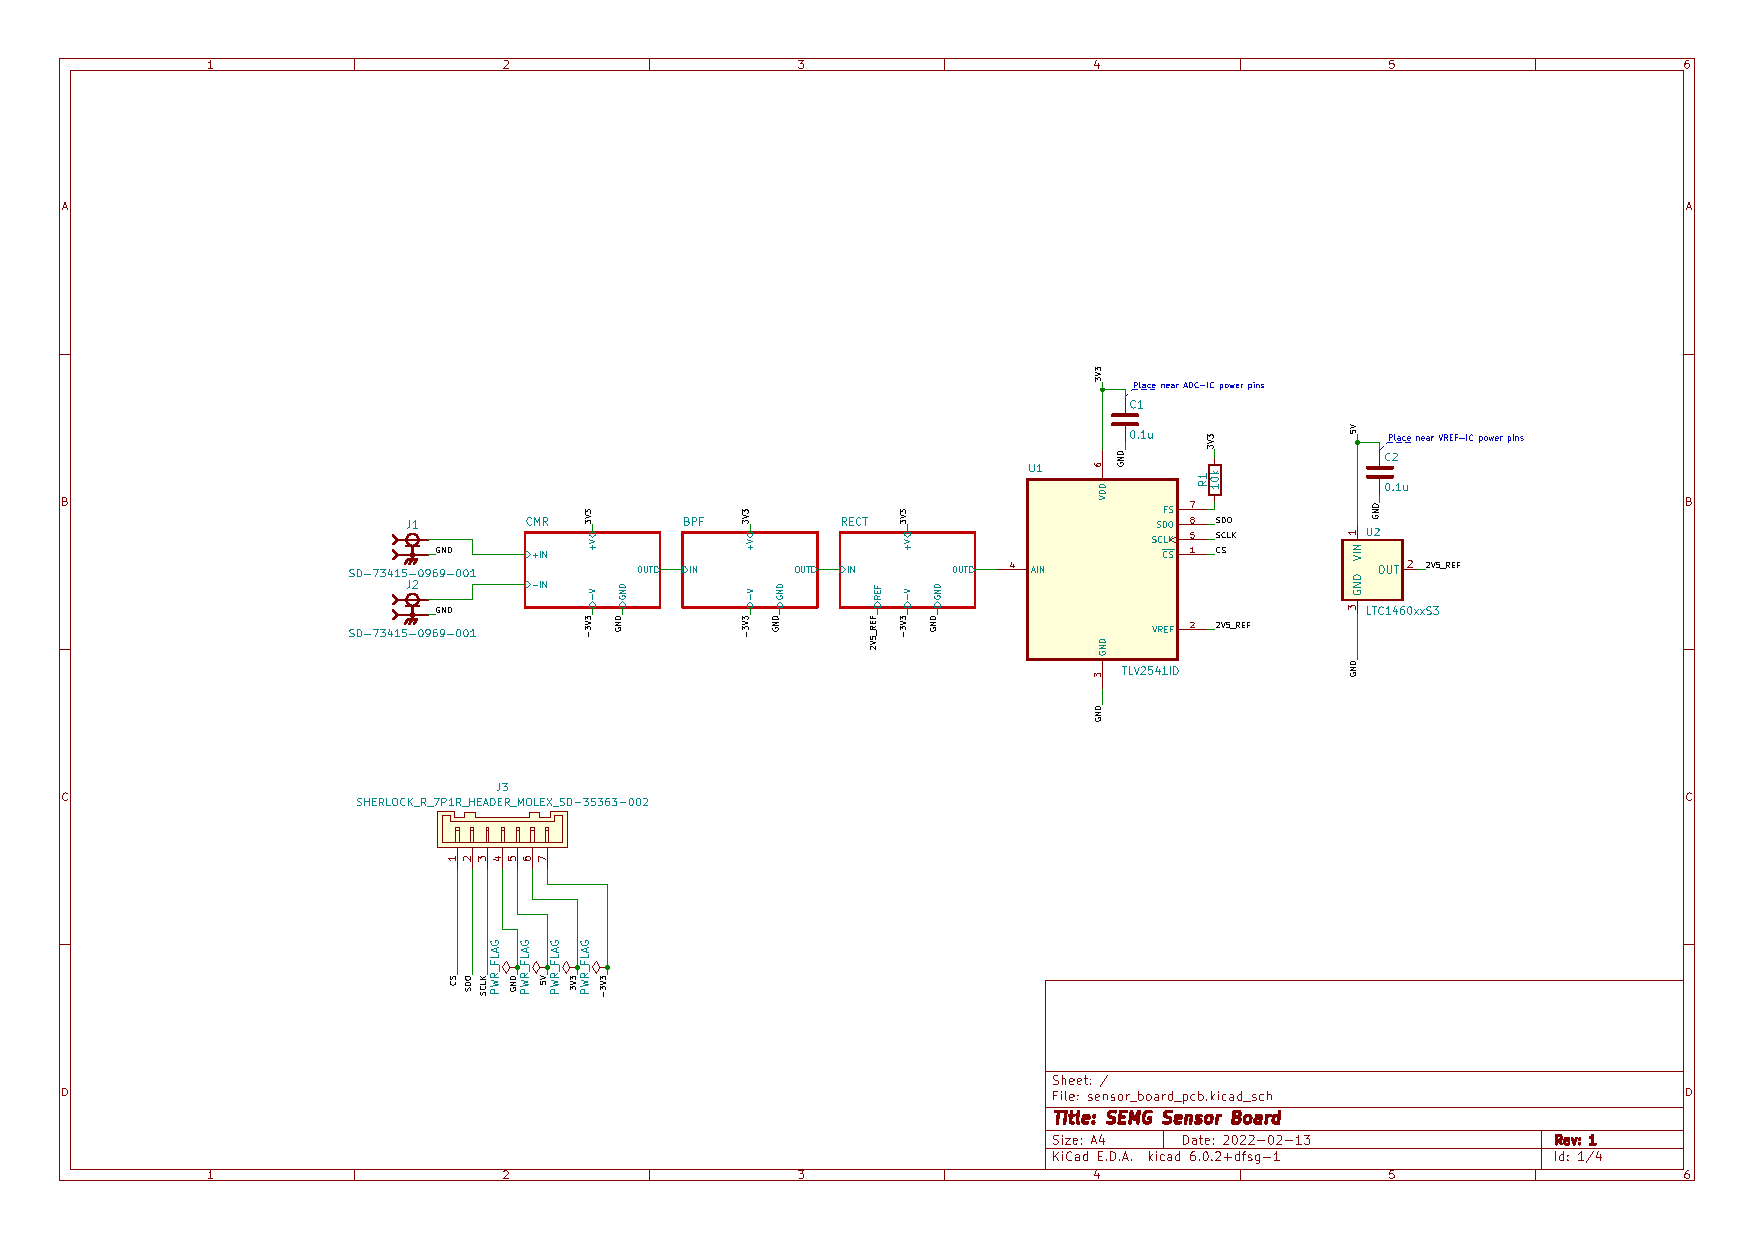
\includegraphics[height=\textwidth, angle=90]{media/sensor_board_pcb.pdf}
        \caption{Circuito pi\`{u} importante gerarchialmente della scheda sensore, che contiene tre nodi \emph{(CMR, BPF, RECT)} presentati nelle segueni Figure \ref{fig:CircuitDiagramSensorBoardCMR}, \ref{fig:CircuitDiagramSensorBoardBPF}, \ref{fig:CircuitDiagramSensorBoardRECT} e un ADC}
        \label{fig:CircuitDiagramSensorBoard}
    \end{figure}
    \begin{figure}[H]
        \begin{minipage}[H]{\linewidth}
            \centering
            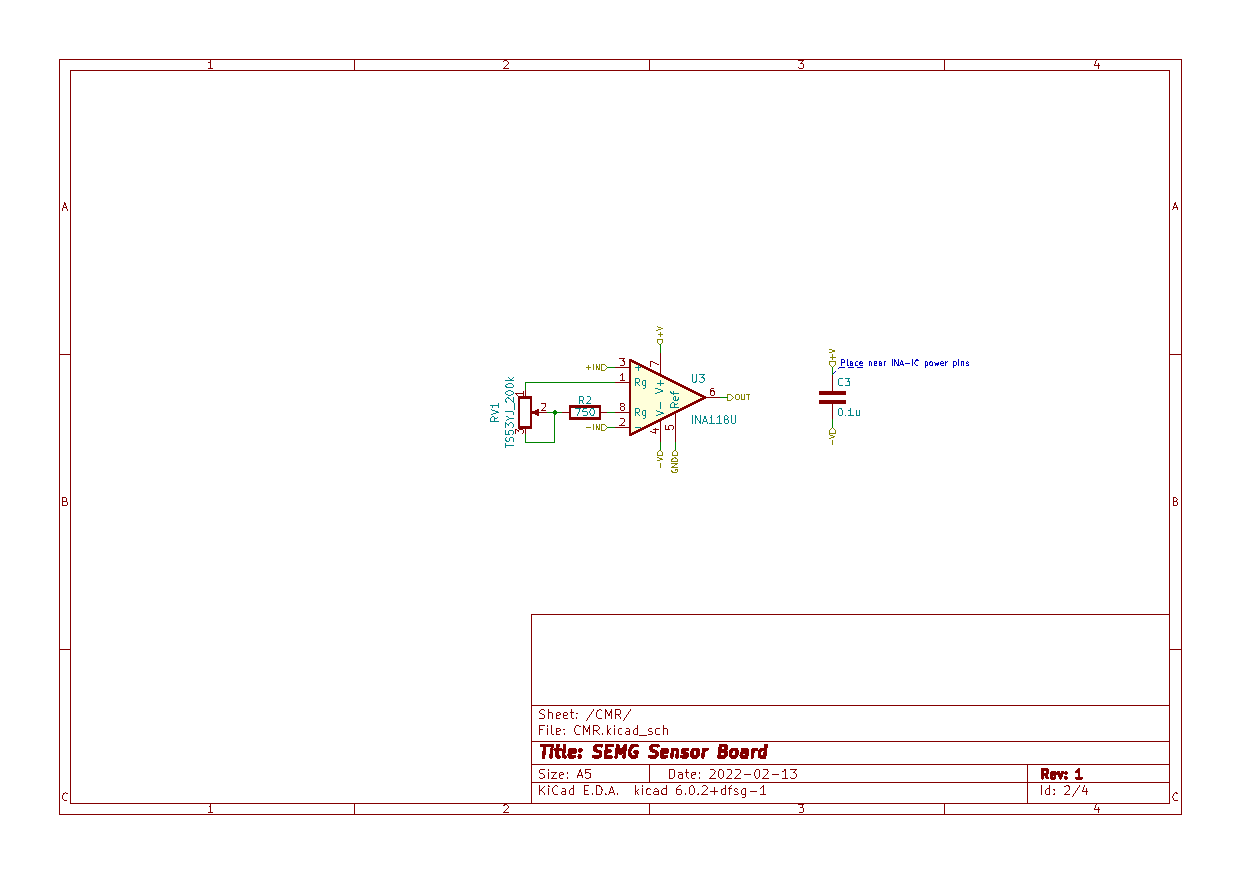
\includegraphics[width=\textwidth]{media/sensor_board_pcb-CMR.pdf}
            \subcaption{Circuito composto da un INA filtrare le parti del segnale differenti ed attenuare le parti identiche}
            \label{fig:CircuitDiagramSensorBoardCMR}
        \end{minipage}
        \begin{minipage}[H]{\linewidth}
            \centering
            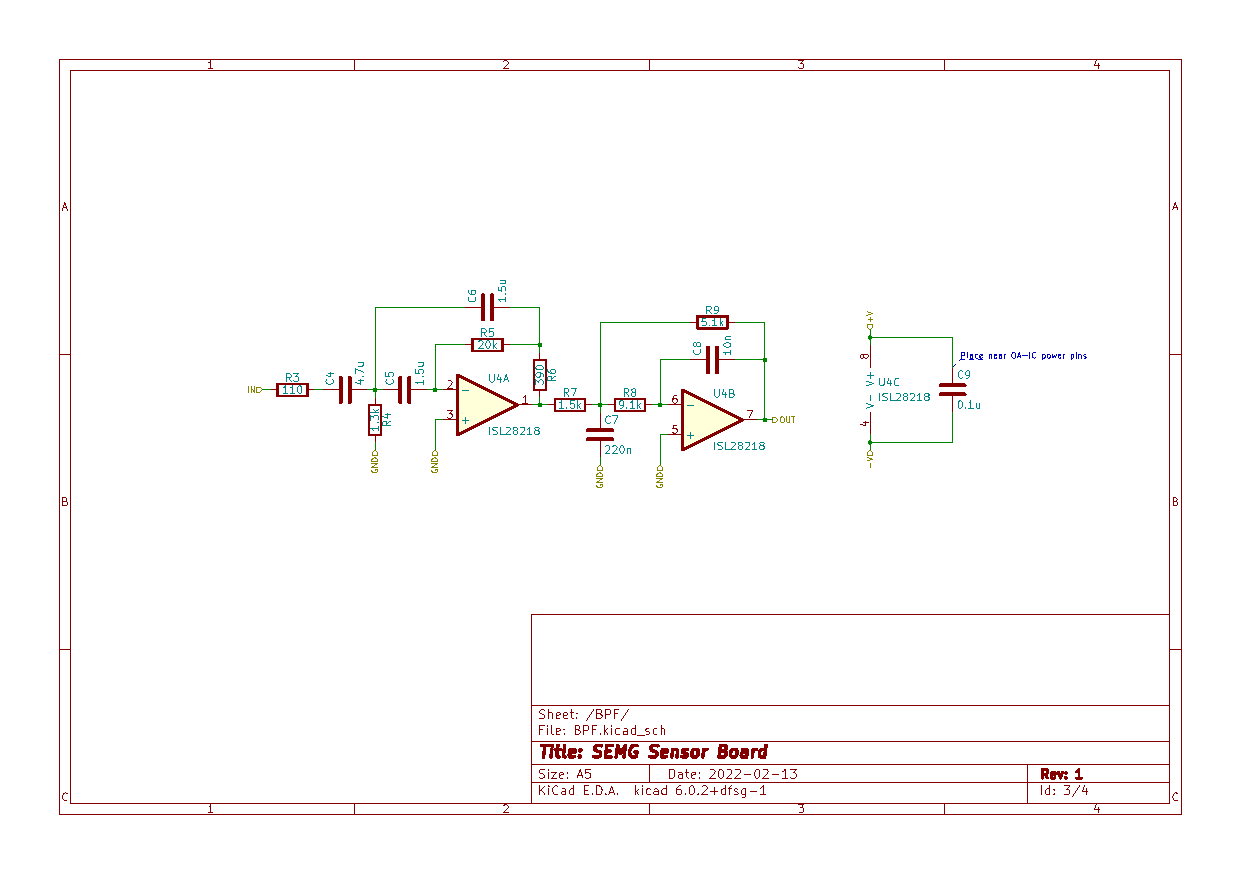
\includegraphics[width=\textwidth]{media/sensor_board_pcb-BPF.pdf}
            \subcaption{Circuito composto da un filtro HPF e un LPF di topologia MFB per filtrare la banda del segnale $20-500Hz$  \emph{(Il circuito inverte due volte il segnale)}}
            \label{fig:CircuitDiagramSensorBoardBPF}
        \end{minipage}
        \caption{}
        \label{fig:CircuitDiagramSensorBoardCMRBPF}
    \end{figure}
    \begin{figure}[H]
        \centering
        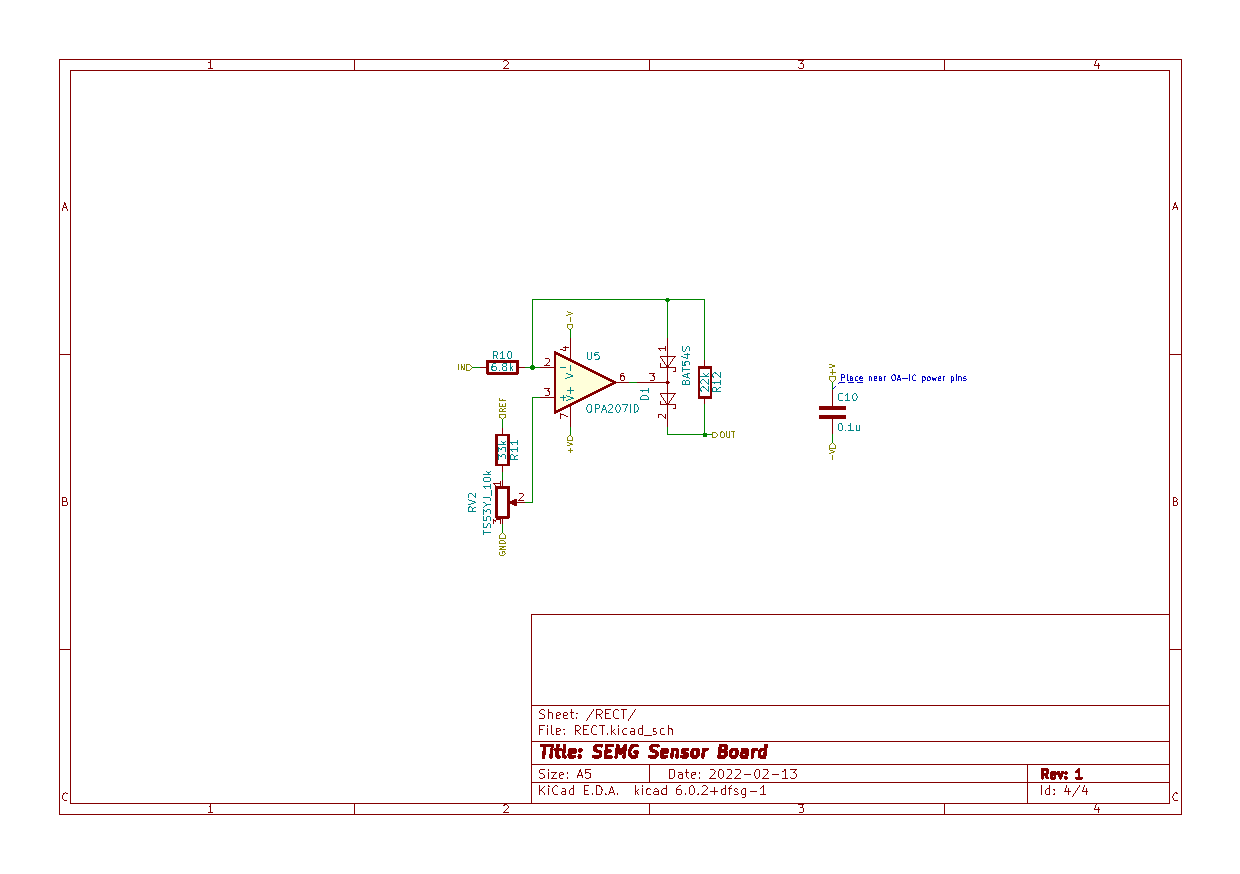
\includegraphics[width=\textwidth]{media/sensor_board_pcb-RECT.pdf}
        \caption{Circuito per rettificare il segnale \emph{(In questa topologia si inverte il segnale e si taglia la sua parte negativa)}}
        \label{fig:CircuitDiagramSensorBoardRECT}
    \end{figure}

    \noindent I circuiti che ho messo sono:
    \begin{itemize}
        \item SEMG Sensor Board --- la scheda del sensore
        \item SEMG Sensor Board - CMR --- la parte dell'INA che ho chiamato in tale modo per Common Mode Rejection oppure rifiuto del segnale nella modalit\`{a} comune
        \item SEMG Sensor Board - BPF --- la parte della filtrazione di frequenze che serve a filtrare la banda di frequenze $20-500Hz$
        \item SEMG Sensor Board - RECT --- la parte della rettificazione del segnale\footnote{L'ADC non pu\`{o} ricevere la tensione negativa minore di $0.3V$ \parenciteit{p8}{TLV2541:Datasheet}}
    \end{itemize}
    Il circuito funziona da due sorgenti, una negativa e una positiva, servono all'INA per mettere la tensione di riferimento al livello del corpo e per adoperare il segnale quando utilizziamo un filtro HPF\footnote{Tutte le componenti delle frequenze basse e della corrente continua vengono filtrate, centrarndo il segnale attorno i $0V$}.
    Ho aggiunto il circuito con nome "SEMG Sensor Board - RECT" per non eccedere i limiti di tensione dell'ADC, anche se il segnale pu\`{o} essere centrato attorno un valore tra i $2.5-0V$\footnote{I $2.5V$ sono dati dal regolatore LTO fisso di $2.5V$ $U2$} dato dal potenziometro $RV2$.
    L'ampiezza del segnale \`{e} aggiustata dal potenziometro $RV1$\footnote{All'ultimo momento ho scoperto che i valori di amplificazione che ho calcolato erano imprecisi e ho variato il valore della resistenza $R2$ dai $10k\Omega$ ai $750\Omega$ in tale modo aumentando il massimo coefficiente di amplificazione del circuito}.
    Le altre modifiche che si possono notare del circuito concettuale proposto in grande parte della Sezione \ref{sec:FilterTheory}, sono le resistenze $R3$ ed $R6$\footnote{Le resistenze sono due per non modificare la funzione di trasferimento}\:\footnote{I valori di queste resistenze sono stati ottenuti dalle simulazioni in KiCad con il metodo del tuning (a tentativi)}che servono a limitare la massima corrente che pu\`{o} fluire dall'output dell'amplificatore $U4A$ o l'INA $U3$ a delle frequenze altissime, che riducono l'Impedenza dei condensatori $C6$ e $C4$ potendo in tale modo causare un malfunzionamento dell'$U3$ o dell'$U4A$.
    Inoltre si nota la presenza dei condensatori $C1$, $C2$, $C3$, $C9$, e $C10$ che hanno il loro nome: bypass capacitors, hanno la funzione di soppressione di rumori di alta frequenza nelle linee di alimentazione, che possono provenire dalla parte digitale del circuito\footnote{Non solo dall'ADC, ma anche dalla parte della sorgente, che viene connessa attrverso il connettore $J3$}.
    L'ADC possiede tre pin, che servono a trasmettere le informazioni con il protocollo SPI, che sono connessi al connettore $J3$.
    Gli altri due connettori $J1$ e $J2$ servono a connettere i cavi degli elettrodi\footnote{Sono connessi al GND per il motivo che il cavo degli elettrodi \`{e} schermato per ridurre le interferenze e perch\'{e} gli elettrodi hanno due contatti: uno di riferimento e uno del segnale stesso}
    L'$R1$ \`{e} una formalit\`{a} dettata dal datasheet dell'ADC\footcite[p5,p21]{TLV2541:Datasheet} per farli capire in che modalit\`{a} deve operare.

    \subsubsection{Scelta componenti}
    Avendo le formule dei filtri e i dati dei datasheet dei componenti ho scelto\footnote{La scelta dei componenti \`{e} stata effettuata sempre col "modus operandi" iterativo con l'aiuto del database dei componenti del mercato di scelta \parencite[]{Mouser:Web}} dei componenti passivi col metodo dei tentativi per equilibrare diversi fattori come i rumori\footnote{Nei calcoli nella Sezione \ref{sec:Calculations}, ho utilizzato solo componenti con i dati del loro White noise o rumore bianco (uguale in tutto lo spettro) e Pink o Flicker noise, rumore rosa (pi\`{u} pronunciato nelle frequenze basse)} che vengono generati dal circuito.

    In seguito ho iniziato a fare delle simulazioni del circuito per ottenere valori dei componenti passivi in scale E standardizzate e che siano maggiormente dei valori uguali per ridurre il BOM\footnote{Bill of Materials, un termine per indicare la lista dei componenti da acquistare per potere comporre il circuito}, ma senza fare dei compromessi sui parametri predefiniti\footnote{Amplificazione, frequenze di taglio nei filtri e i rumori dei componenti (la dimensione dei rumori viene definita nei calcoli della Sezione \ref{sec:Calculations})}.

    \begin{figure}[H]
        \centering
        \begin{minipage}[H]{\linewidth}
            \centering
            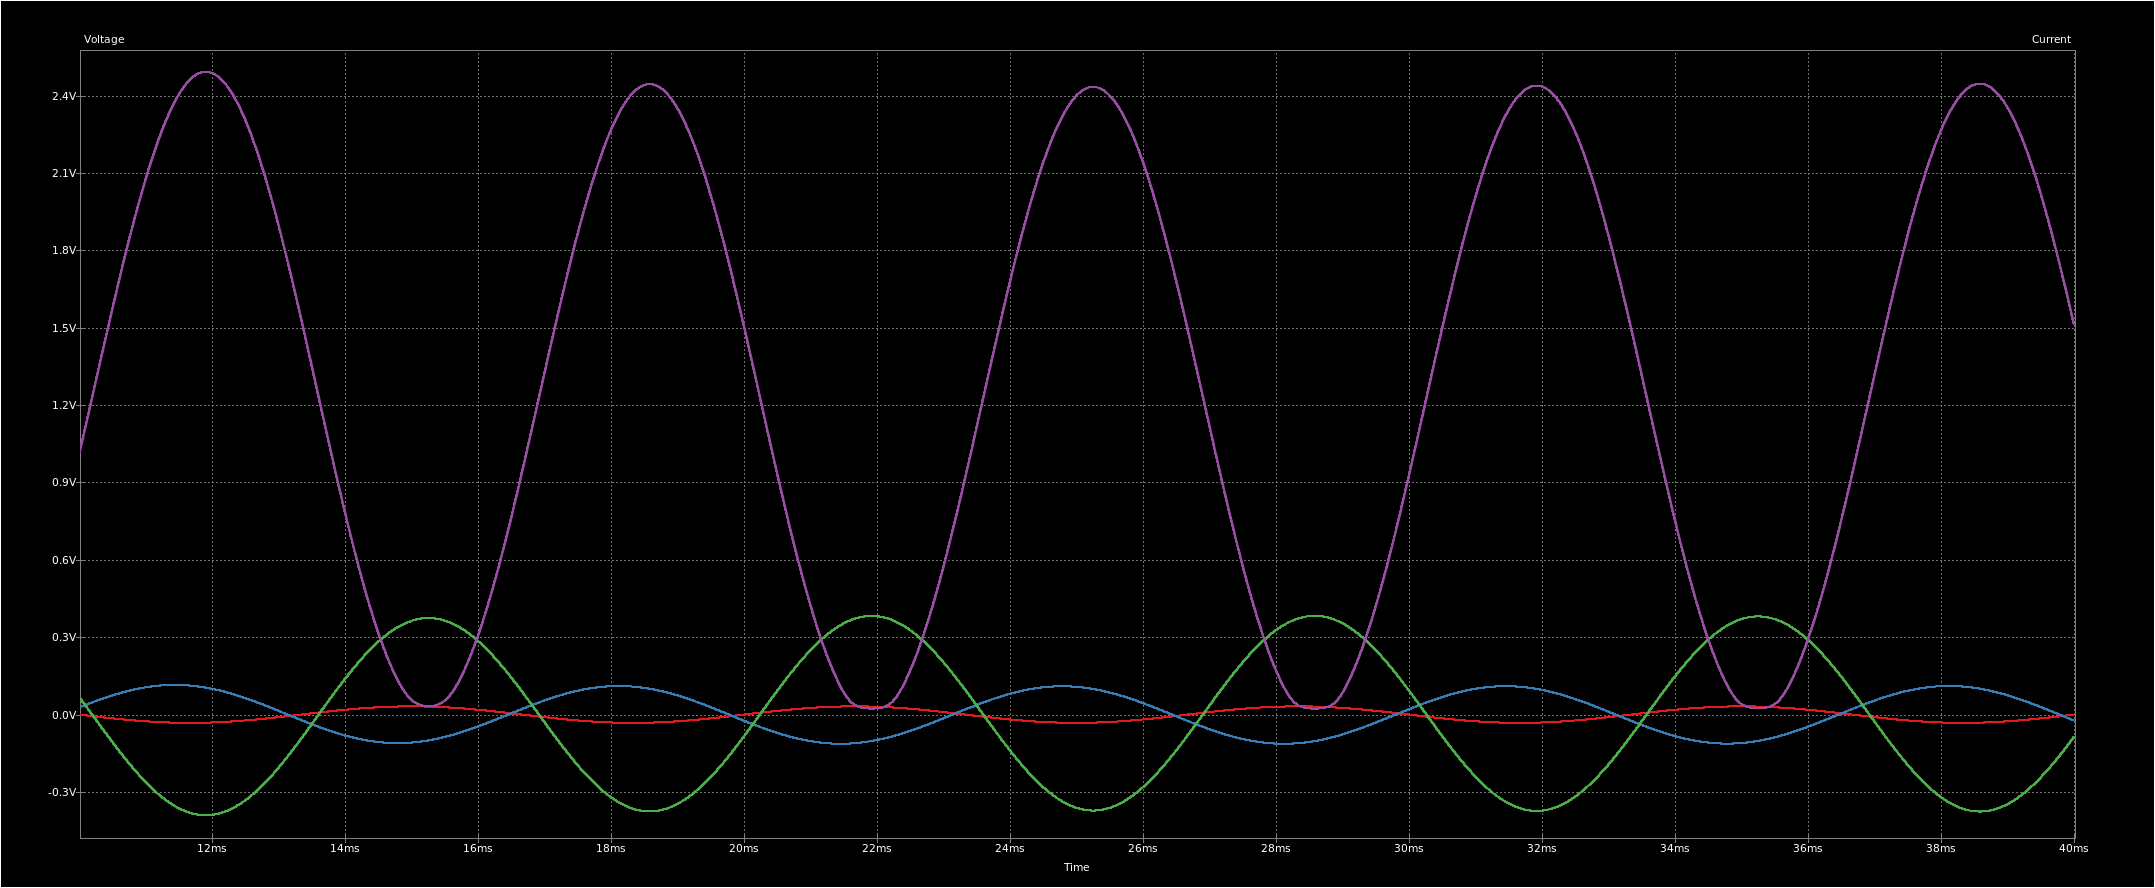
\includegraphics[width=\linewidth]{media/simtimeresp.png}
            \subcaption{Risposta della simulazione del circuito nel tempo, con il segnale rosso all'uscita del nodo dell'ipotetico INA \emph{($SIG\_IN$)}, con il segnale blu all'uscita del HPF \emph{(Uscita di $U1$)}, con il segnale verde all'uscita del LPF \emph{(Uscita di $U2$)} e con il segnale viola all'usicta del rettificatore \emph{($SIG\_OUT$)} \emph{(In questo caso il segnale d'entrata nel nodo dei filtri di frequenza \`{e} di $32mV$ con frequenza di $150Hz$, che \`{e} stato centrato all'ultimo nodo attorno $1.25V$)}}
            \label{fig:timeresp}
        \end{minipage}
        \\
        \begin{minipage}[H]{\linewidth}
            \centering
            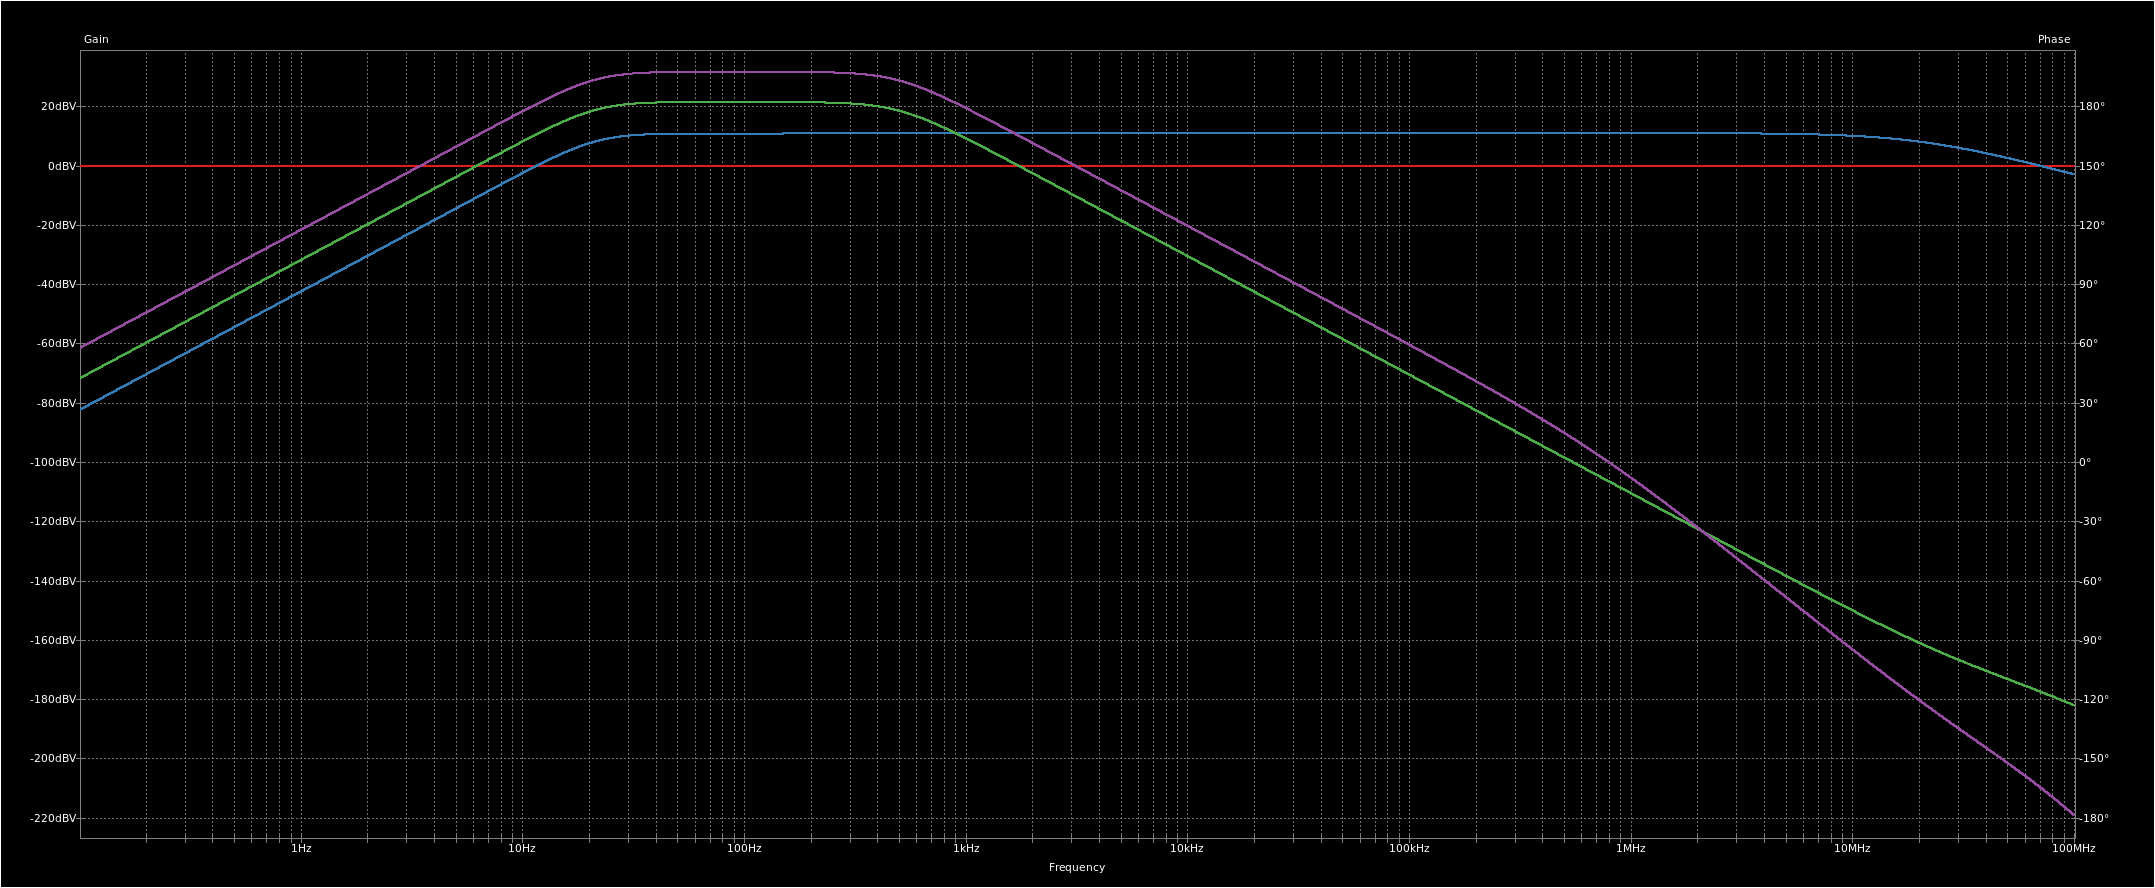
\includegraphics[width=\linewidth]{media/simfreqresp.png}
            \subcaption{Risposta del circuito nello spettro delle frequenze con il segnale rosso all'uscita dell'ipotetico INA \emph{($SIG\_IN$)}, con il segnale blu all'uscita del HPF \emph{(Uscita di $U1$)}, con il segnale verde all'uscita del LPF \emph{(Uscita di $U2$)} e con il segnale viola all'usicta del rettificatore \emph{($SIG\_OUT$)}}
            \label{fig:freqresp}
        \end{minipage}
        \caption{Grafici descriventi il comportamento del filtro nella simulazione}
        \label{fig:freqtimeresp}
    \end{figure}

    \begin{figure}[H]
        \centering
        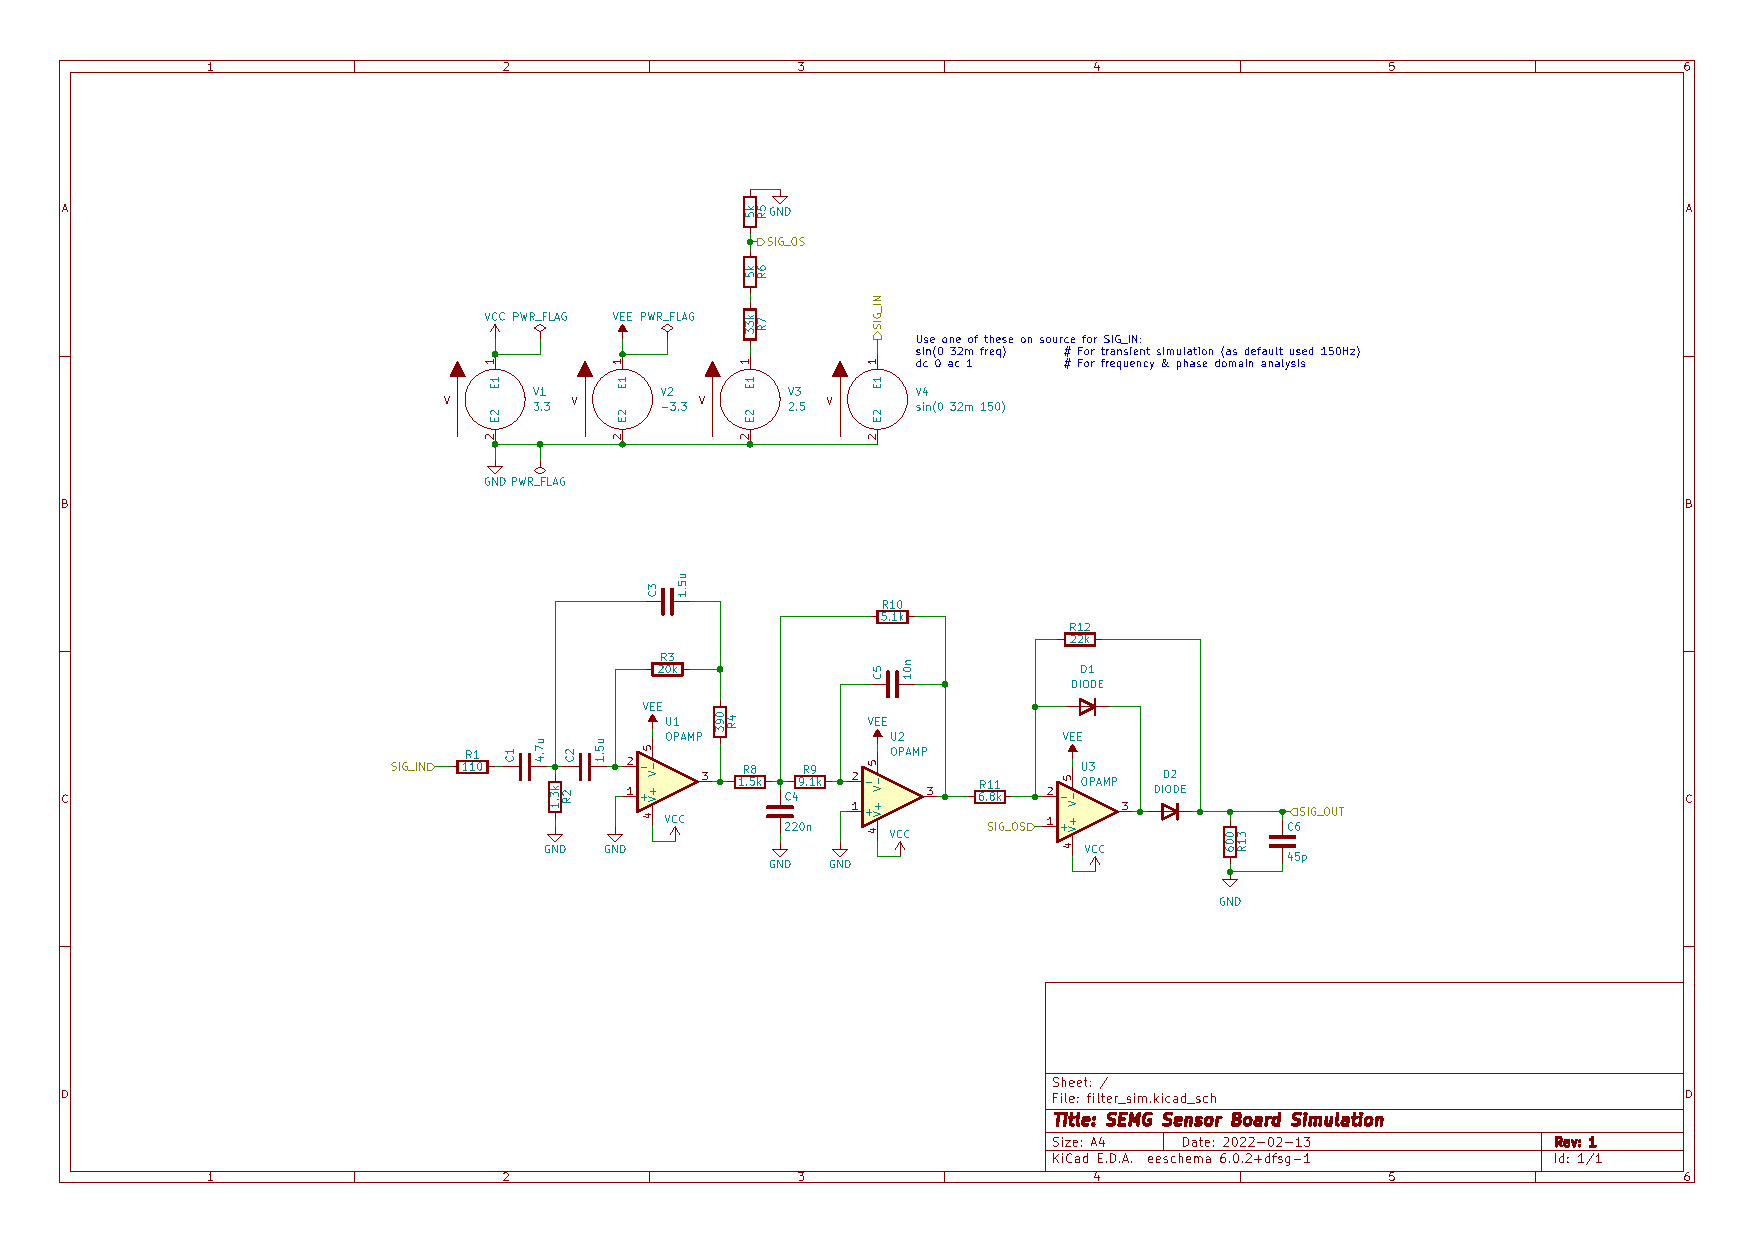
\includegraphics[height=\textwidth, angle=90]{media/filter_sim.pdf}
        \caption{Il circuito nel quale sono state fatte le simulazioni}
    \end{figure}

    \noindent Per prima cosa ho scelto l'ADC che era adatto alla tensione della logica di $3.3V$ e di risoluzione $12bit$\footnote{Con l'SNR (Signal to Noise Ratio o coefficiente della potenza del segnale a confronto con la potenza del rumore) di approssimativamente $72dB$ perch\'{e} \`{e} la risoluzione stessa convertita in $[dB]$, che viene calcolato nella Sezione \ref{sec:Calculations}}.
    \todo{Put more detailed references to calculations (to single files)}

    Per scegliere i componenti attivi\footnote{Si indendono i circuiti integrati menzionati con $UX$ nel circuito in Figure \ref{fig:CircuitDiagramSensorBoard} \ref{fig:CircuitDiagramSensorBoardCMRBPF} \ref{fig:CircuitDiagramSensorBoardRECT}} della parte analogica ho cercato di calcolare i minimi e i massimi per delle diverse caratteristiche per ogni componente, come GBPW\footnote{Gain Bandwidth Power, oppure }, slew rate\footnote{La velocit\`{a} di reazione dell'amplificatore, ovvero quanta tensione riesce a variare in un certo intervallo tempo (si misura in $[V/\mu s]$)}, correnti massime dell'output e altri\footnote{Si possono vedere nella Sezione \ref{sec:Calculations}} per gli OA e l'INA per adattarli all'ADC scelto

    \subsubsection{Layout}
    Per il layout\footnote{La disposizione dei componenti e delle traccie che faranno da conduttori} della scheda ho scelto le figure dei componenti simili, ovvero tutti i circuiti integrati sono di formato SOIC-8\footcite[]{SOIC:Wiki}, i diodi e il riferimento di tensione sono di formato SOT-223\footcite[]{SOT:Wiki} e i componenti passivi di dimensione 1608\footnote{Si intende in misura metrica}\:\footcite[]{SMT:Wiki} per poterli comodamente saldare a col saldatore senza compromettere la piccola dimensione del circuito.

    Ovviamente per la scheda ho scelto la variante con il minore numero di strati possibile per diminuire la complessit\`{a} del circuito e la possibilit\`{a} di farlo in casa con il metodo del ferro da stiro\footnote{Se ne racconta nella Sezione \ref{sec:BuildingHardware}} e l'incisione chimica\footnote{Se ne racconta nella Sezione \ref{sec:BuildingHardware}}.
    Inoltre ho dedicato lo strato inferiore per GND per aumentare il decoupling\footnote{Tutti i componenti introducono dei rumori anche nella sorgente quando consumano diverse quantit\`{a} di corrente in istanti diversi} dei componenti come una buona pratica.

    Lo spessore delle tracce era scelto arbitrariamente\footnote{Si pu\`{o} ignorare il contributo dello skin effect \parenciteit{}{SkinEffect:Wiki} per le basse frequenze come con quelle con le quali lavoriamo}

    \begin{figure}[H]
        \centering
        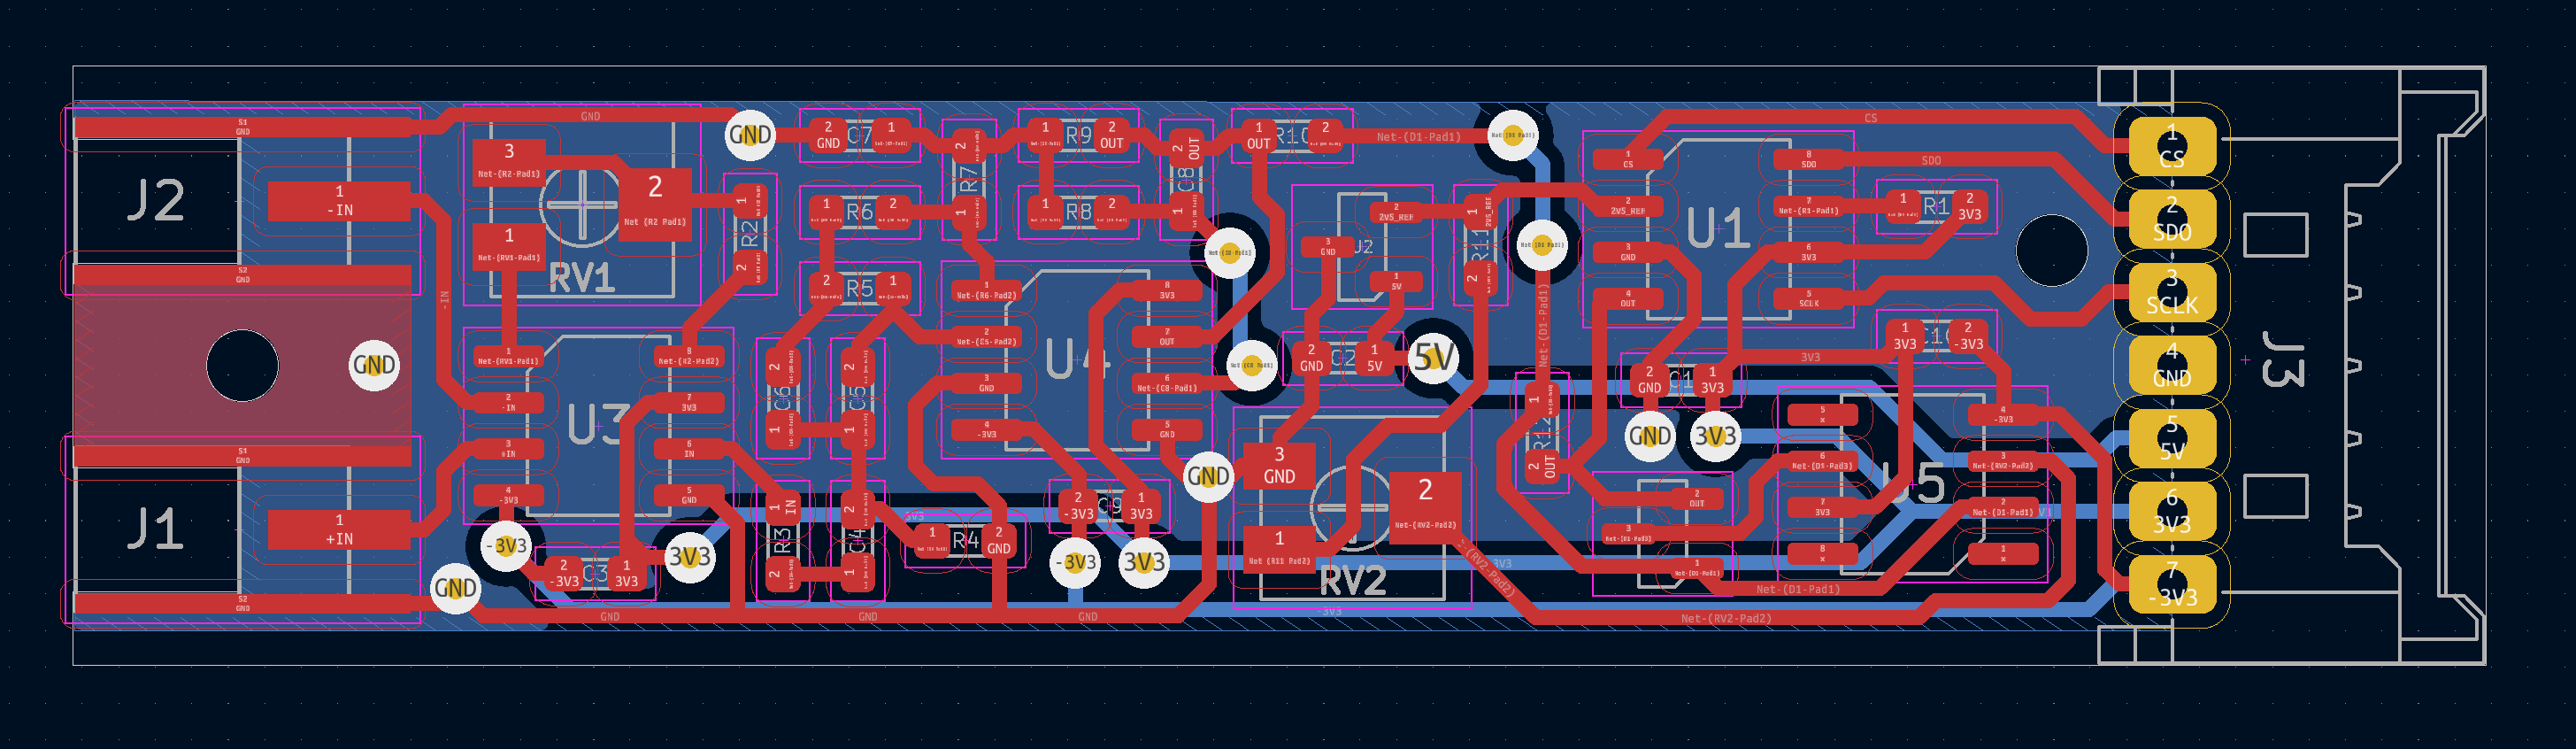
\includegraphics[width=\linewidth]{media/Layout.png}
        \caption{Layout della scheda sensore, la parte conduttiva inferiore della scheda in blu e la parte conduttiva superiore della scheda in rosso, le vias sono dei cerchietti in giallo e bianco}
        \label{fig:Layout}
    \end{figure}
    \clearpage

    \section{Costruzione}\label{sec:Building}
    \subsection{Hardware}\label{sec:BuildingHardware}
    Prima ho stampato su dei fogli di carta da ufficio delle variazioni del circuito\footnote{Figura \ref{fig:BuildingHardwarePaperSheet}}.
    \begin{figure}[H]
        \centering
        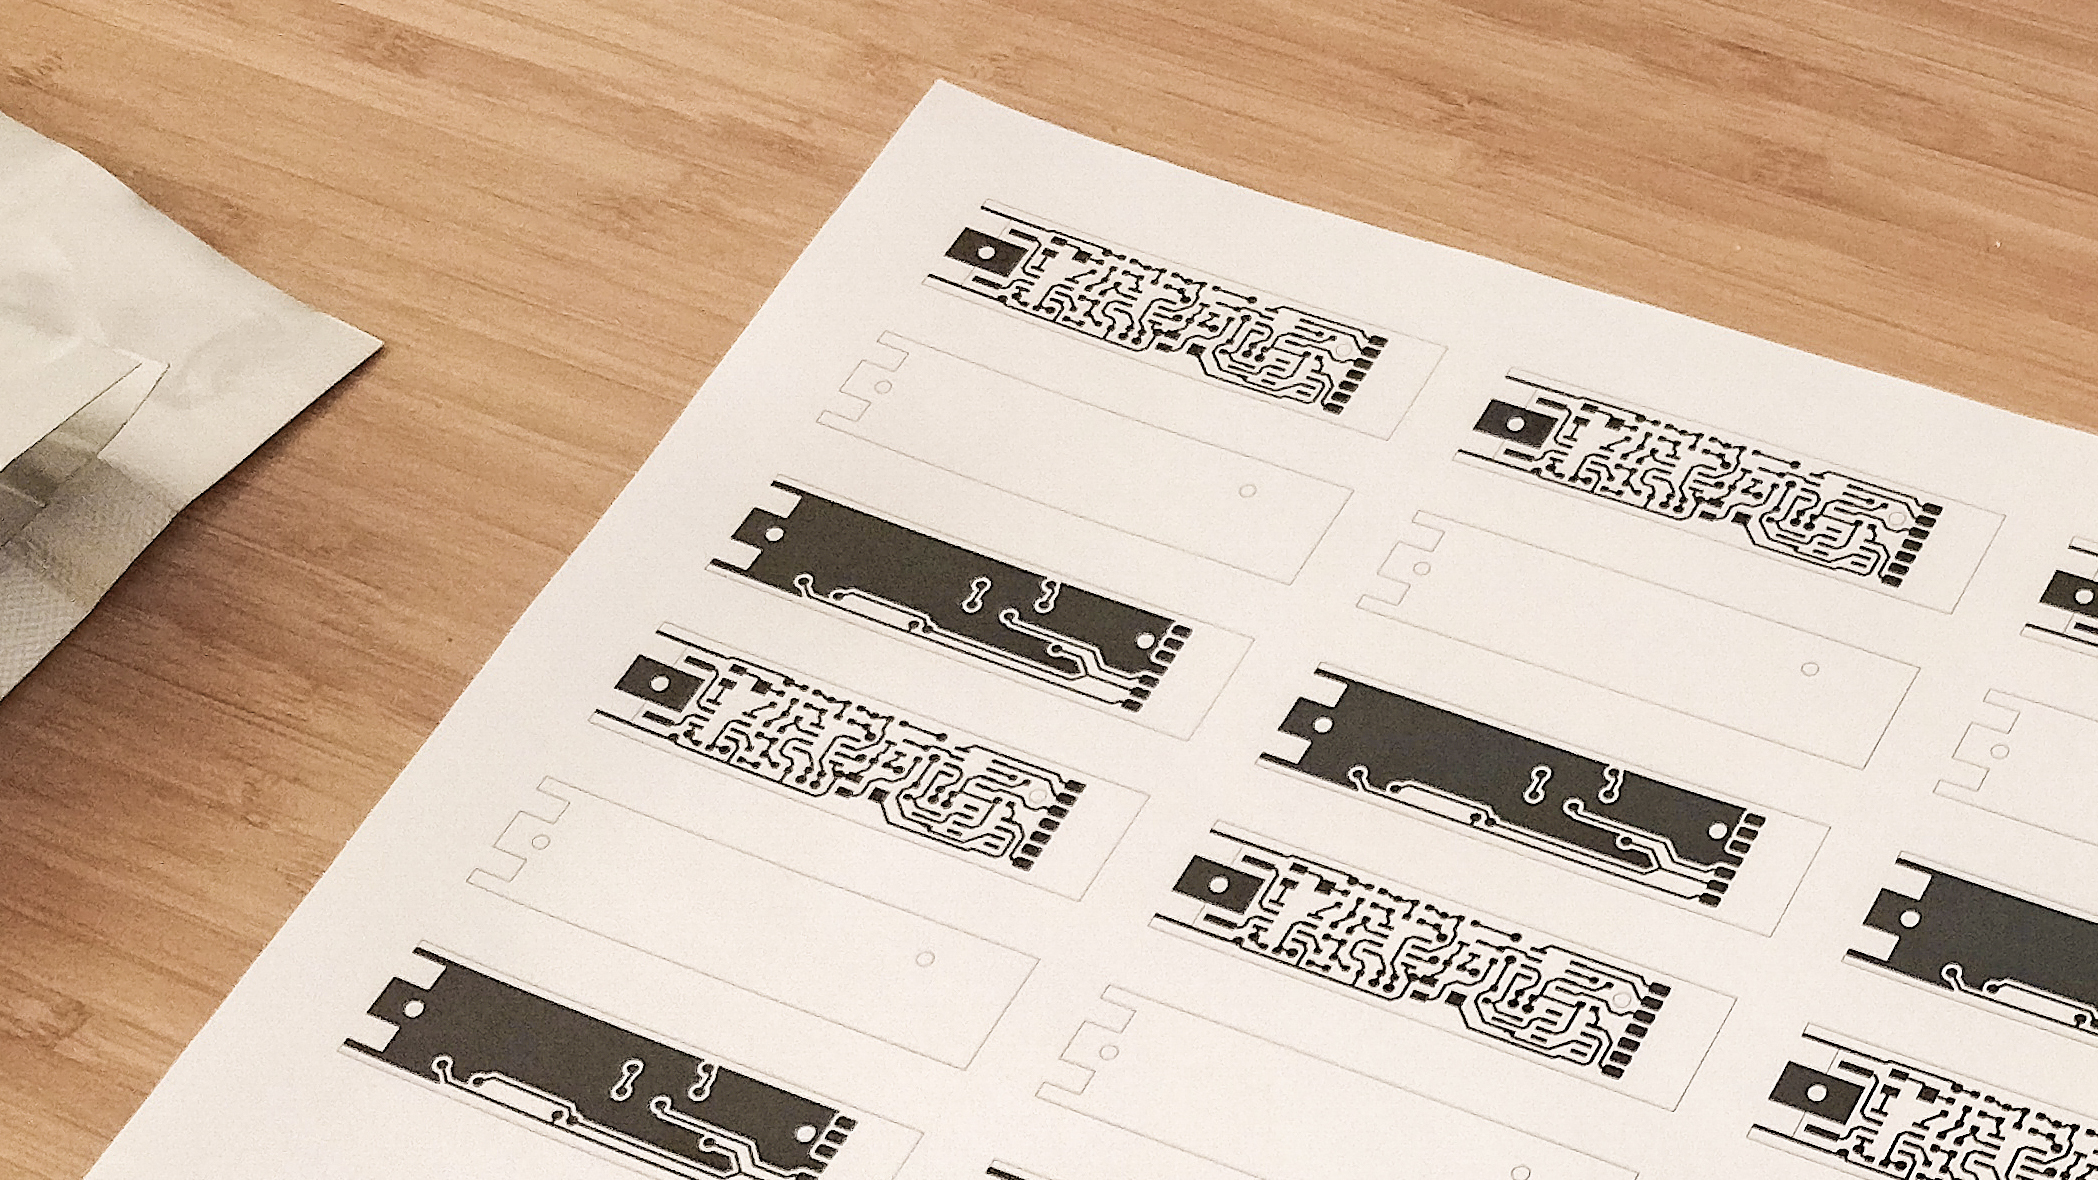
\includegraphics[width=.95\linewidth]{media/album/PSX_20220228_025610.jpg}
        \caption{}
        \label{fig:BuildingHardwarePaperSheet}
    \end{figure}
    Ho scelto in seguito le versioni del circuito che sono uscite meglio e le ho messe da parte per utilizzarle come maschere per l'incisione chimica e quelle uscite peggio, le ho usate come guida per preparare il pezzo della scheda\footnote{Figura \ref{fig:PhotoPCBCut}}.
    La preparazione consisteva nel fare dei fori\footnote{Figura \ref{fig:PhotoPCBDrill}} in delle determinate posizioni per le vias\footnote{Delle connessioni tra i strati della scheda che ho fatto banalmente con un buco e un conduttore del cavo} e nella seguente pulizia della superficie della scheda.

    \begin{figure}[H]
        \centering
        \begin{minipage}[H]{.45\linewidth}
            \centering
            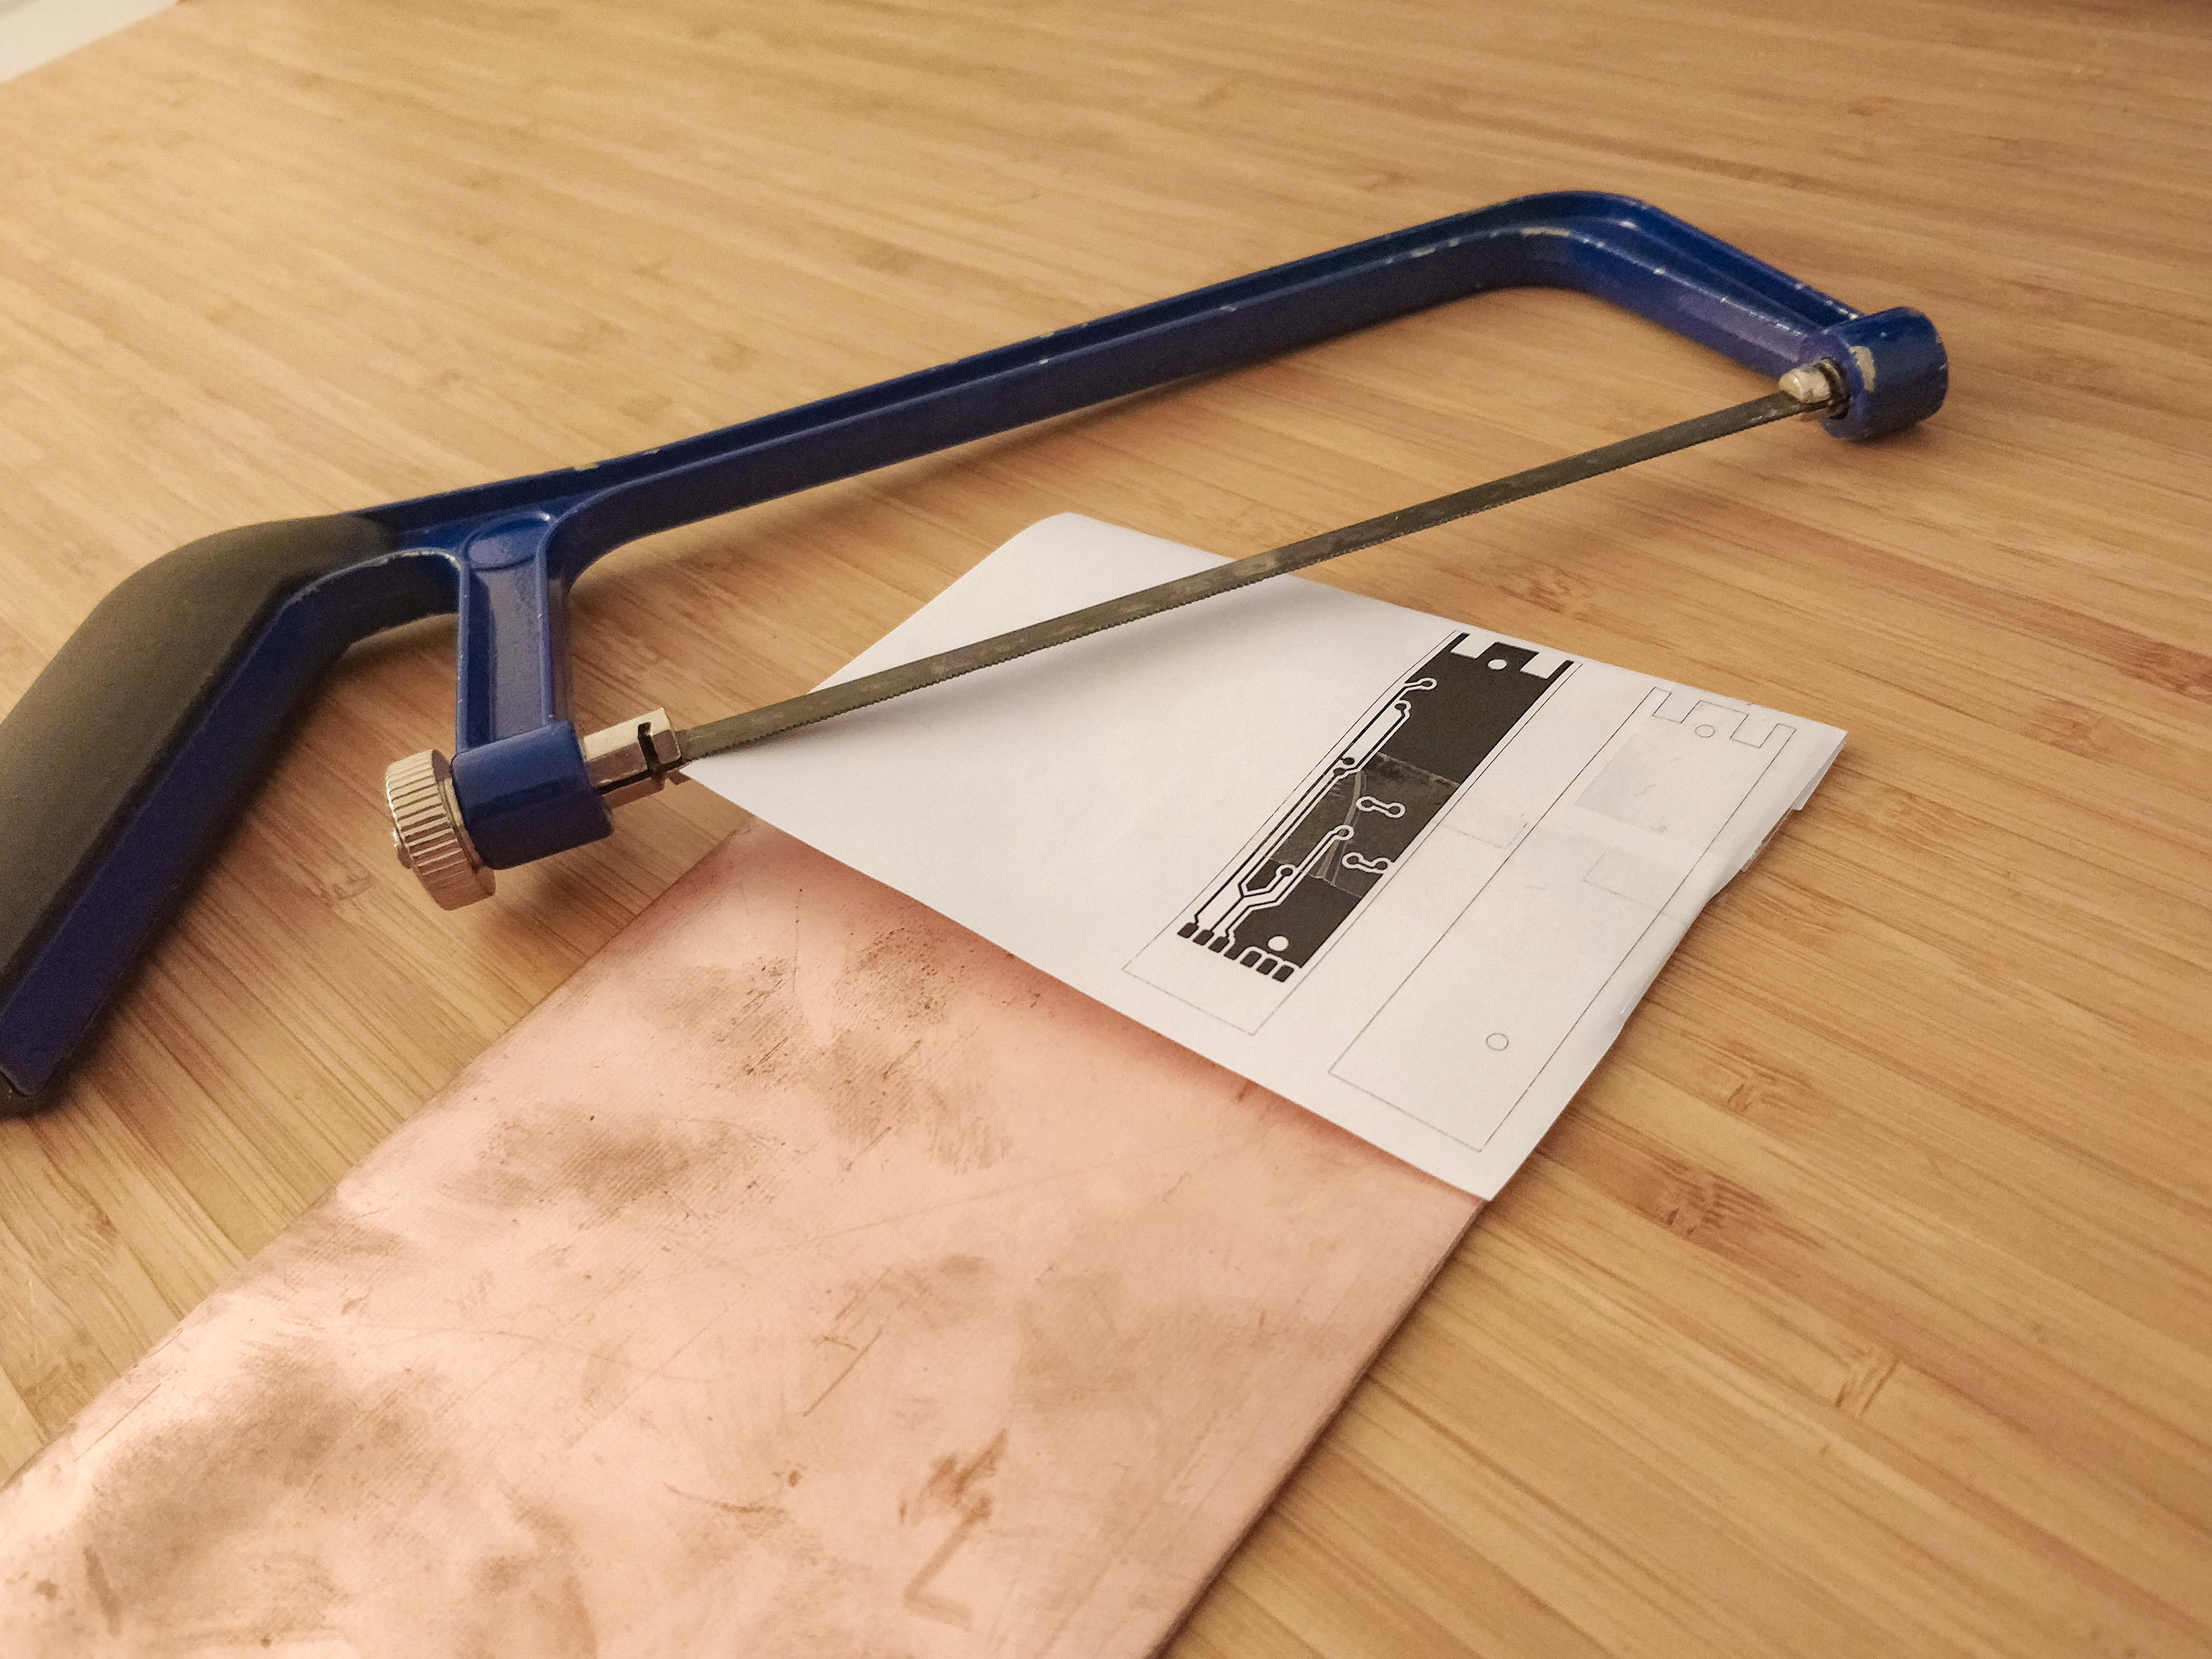
\includegraphics[width=\linewidth]{media/album/PSX_20220228_025933.jpg}
            \caption{}
            \label{fig:PhotoPCBCut}
        \end{minipage}
        \hspace{.04\linewidth}
        \begin{minipage}[H]{.45\linewidth}
            \centering
            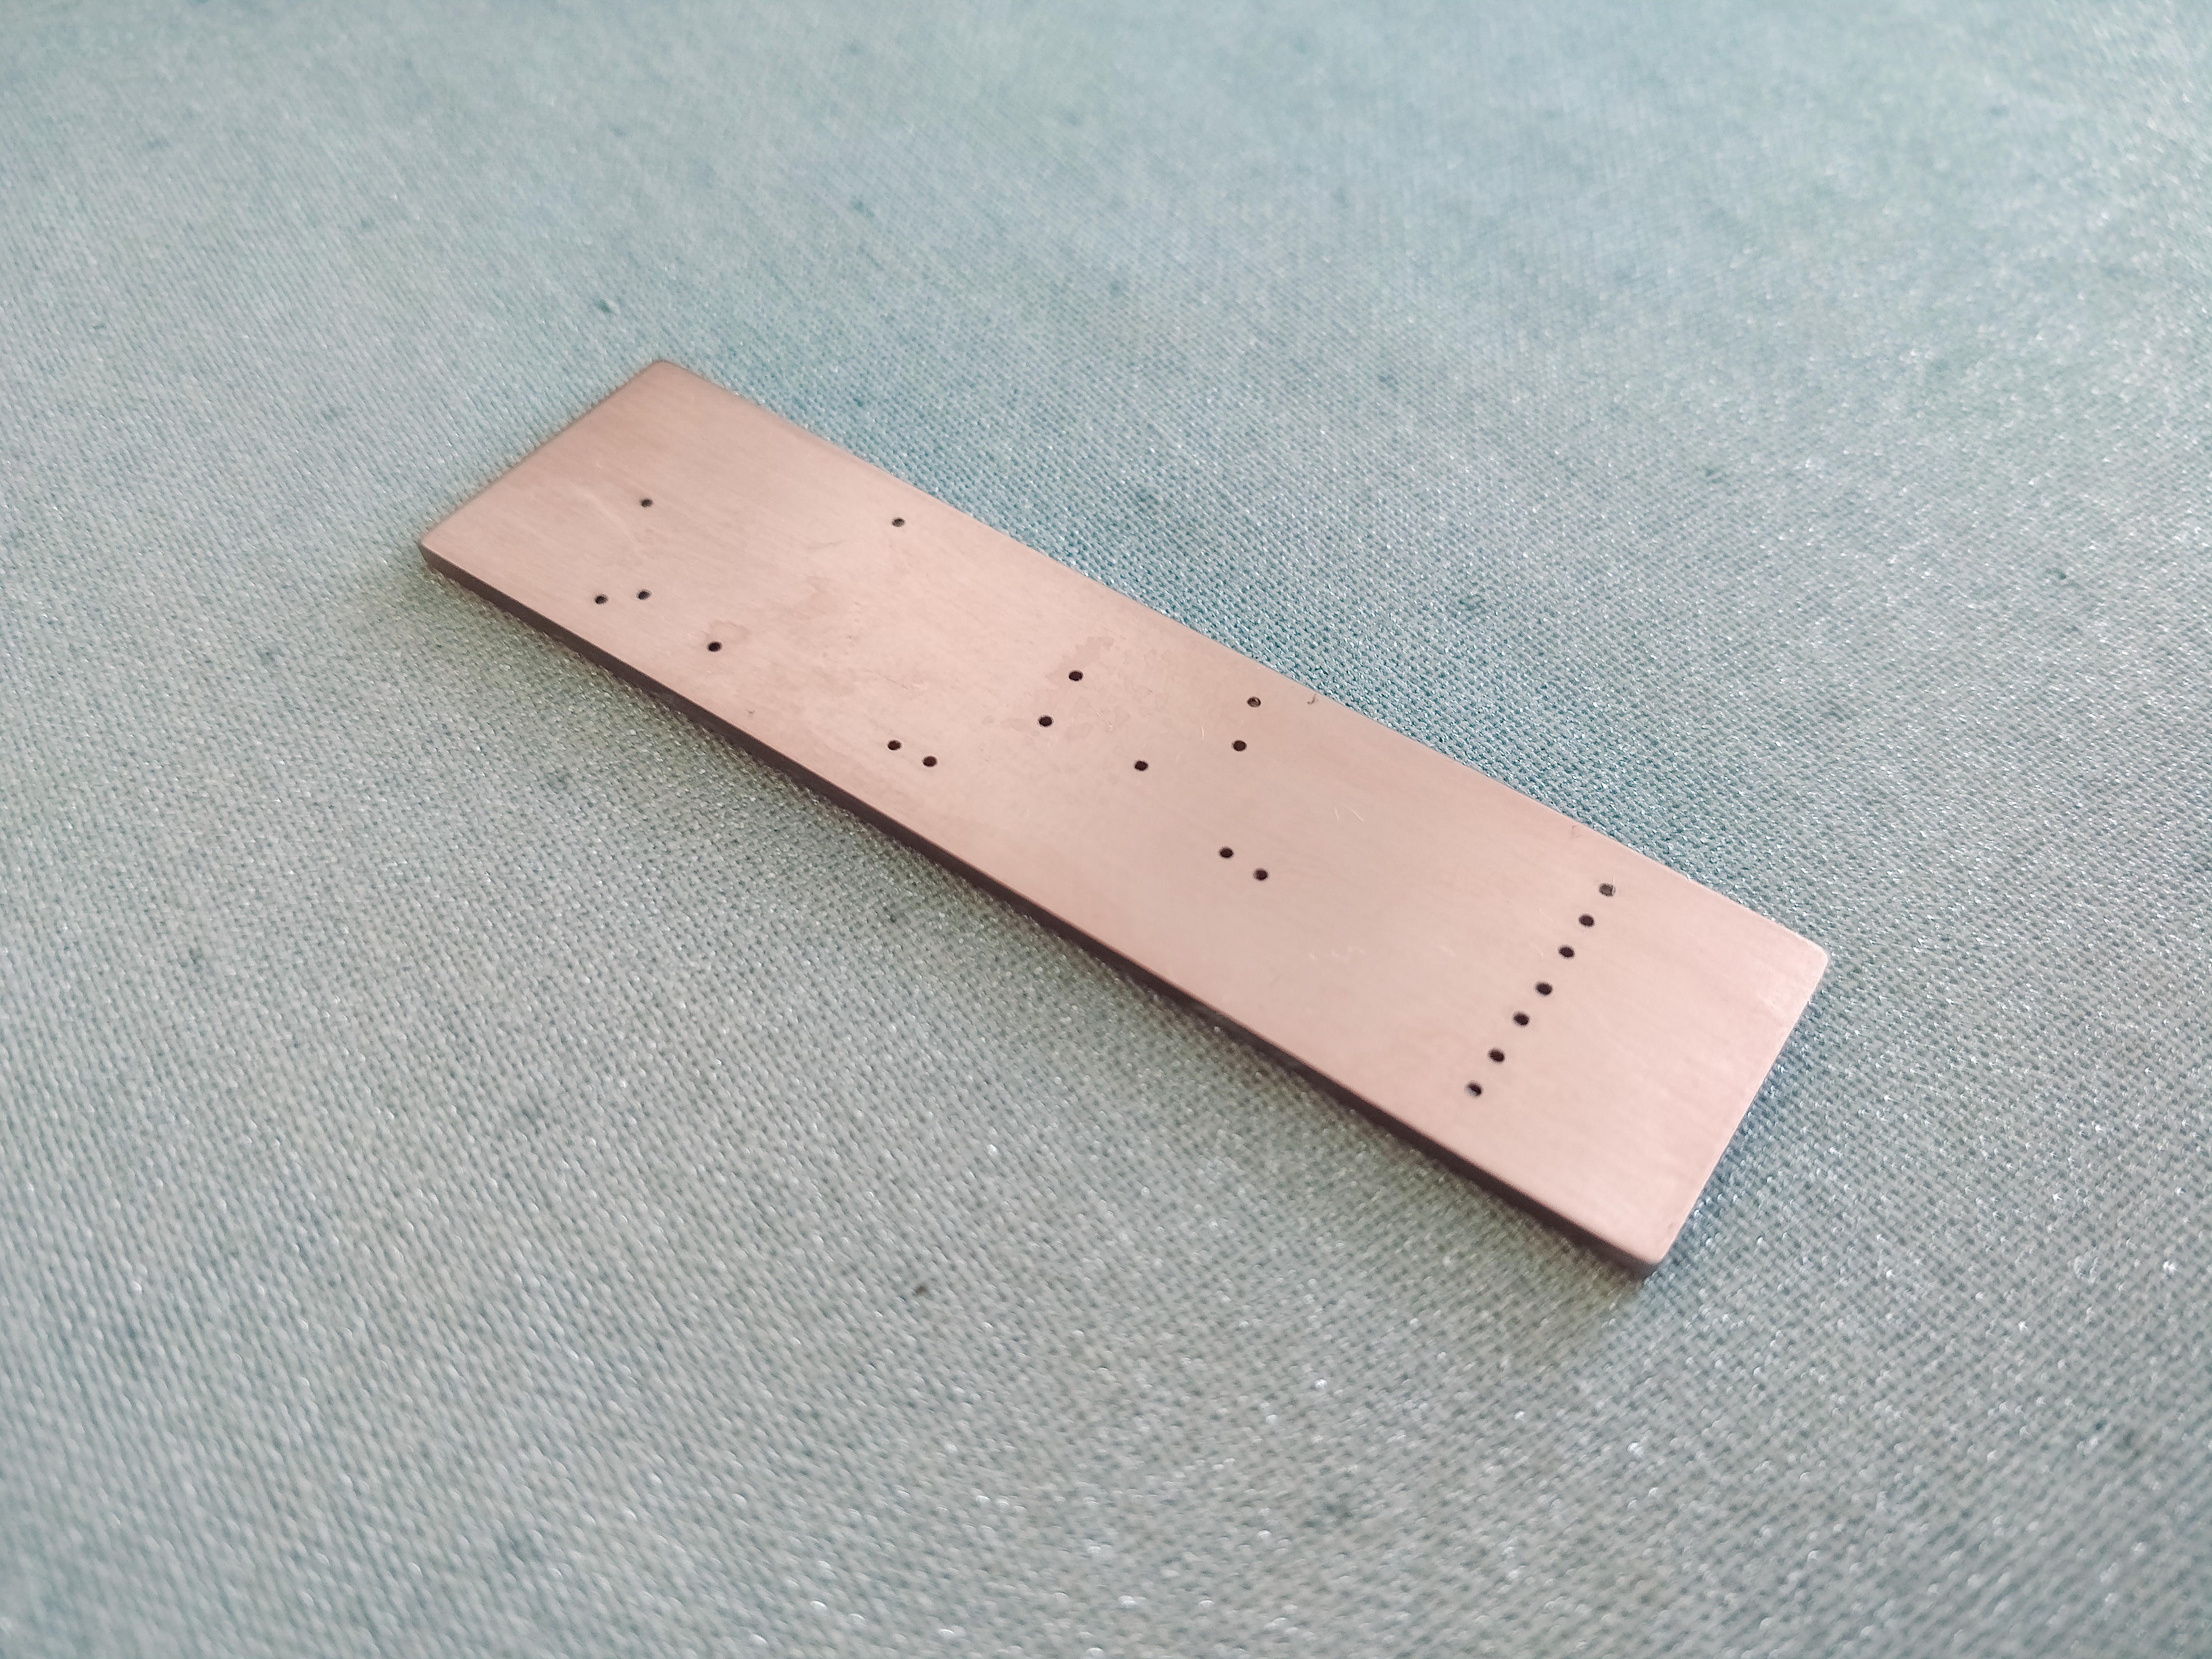
\includegraphics[width=\linewidth]{media/album/PSX_20220228_174045.jpg}
            \caption{}
            \label{fig:PhotoPCBDrill}
        \end{minipage}
    \end{figure}
    \clearpage

    Dopo aver preparato una soluzione\footnote{Figure \ref{fig:PhotoSolutionPrep}, \ref{fig:PhotoSolution}} del 40\%\emph{(m/m)}\footnote{Ho deciso di replicare una soluzione commerciale per l'incisione delle schede \parenciteit{p1}{FECL3:Datasheet}} di FeCl3\footnote{Si deve aggiungere a poco a poco il soluto nella soluzione controllando la sua temperatura che non superi i $55^{\circ}C$ \parenciteit{p2}{FECL3:Datasheet} perch\'{e} avviene un fenomeno esotermico} ho iniziato il processo dell'incisione in un posto ben ventilato\footnote{Nella reazione con il rame si pu\`{o} formare il gas $Cl_2$: $FeCl_3 + Cu \Rightarrow CuCl + FeCl_2$ e in seguito $FeCl_2 + Cu \Rightarrow CuFe + Cl_2$}.

    \begin{figure}[H]
        \centering
        \begin{minipage}[H]{.525\linewidth}
            \centering
            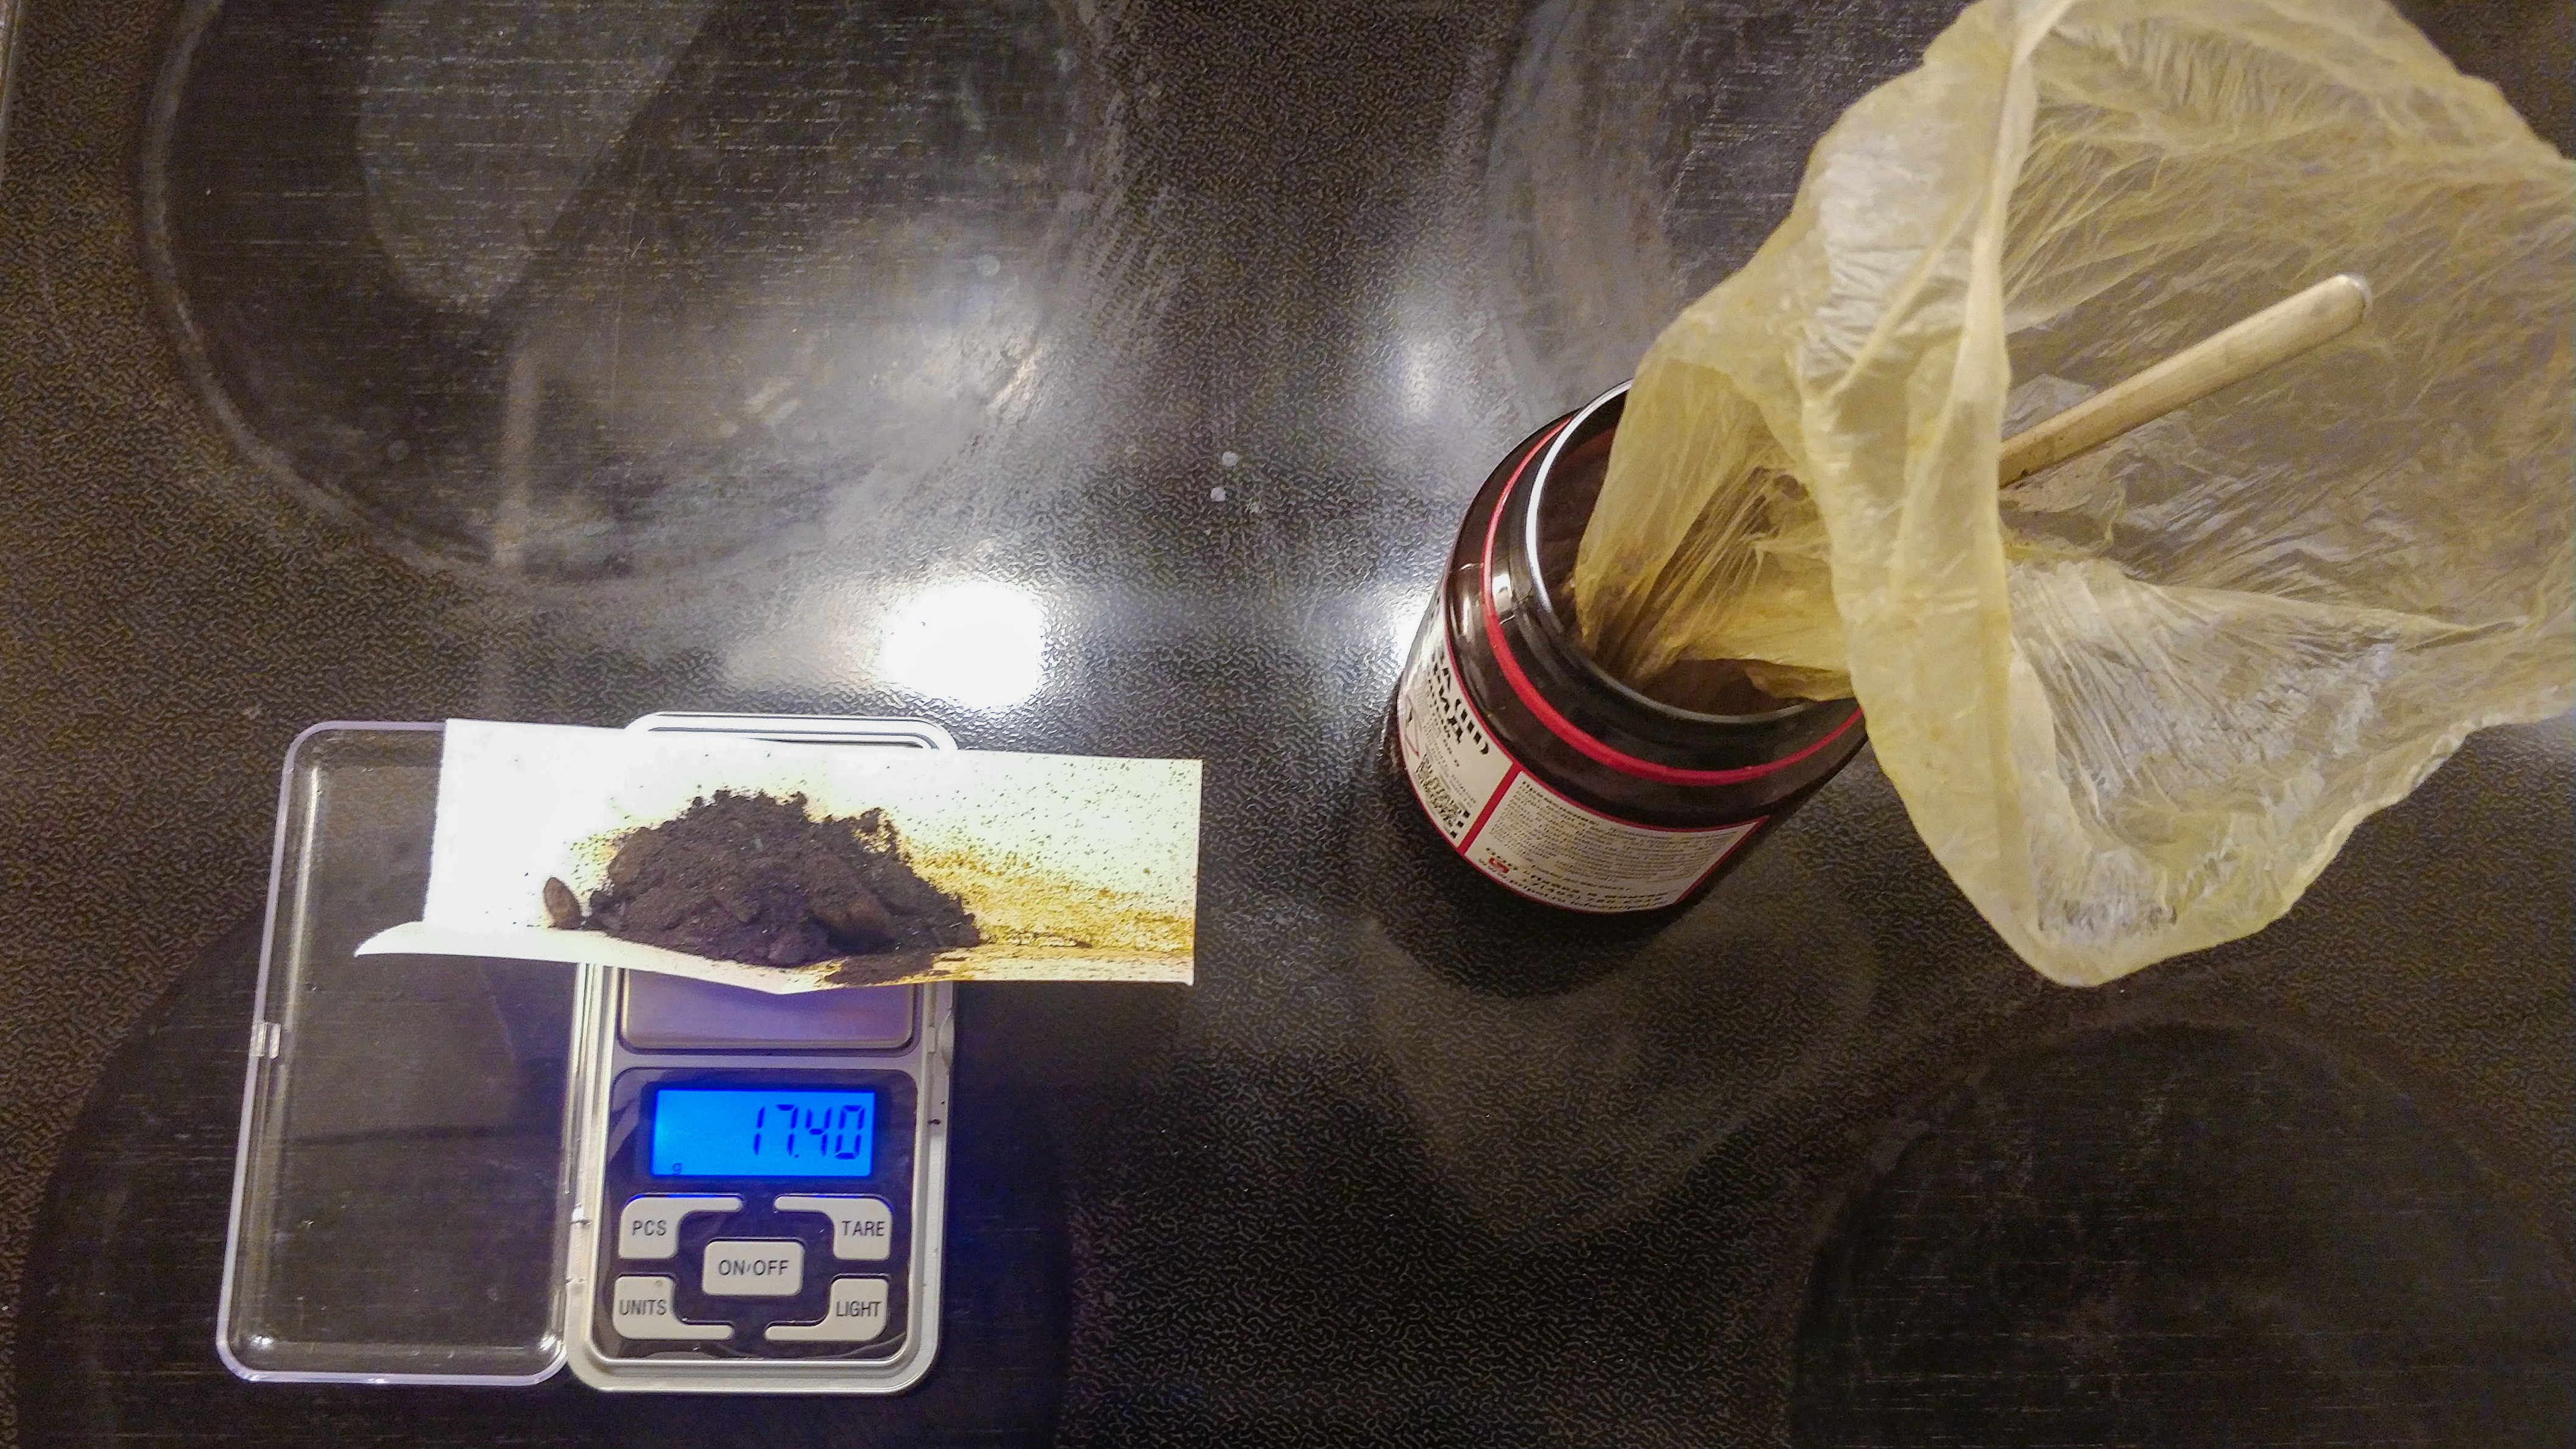
\includegraphics[width=\linewidth]{media/album/PSX_20220228_160724.jpg}
            \caption{}
            \label{fig:PhotoSolutionPrep}
        \end{minipage}
        \hspace{.04\linewidth}
        \begin{minipage}[H]{.394\linewidth}
            \centering
            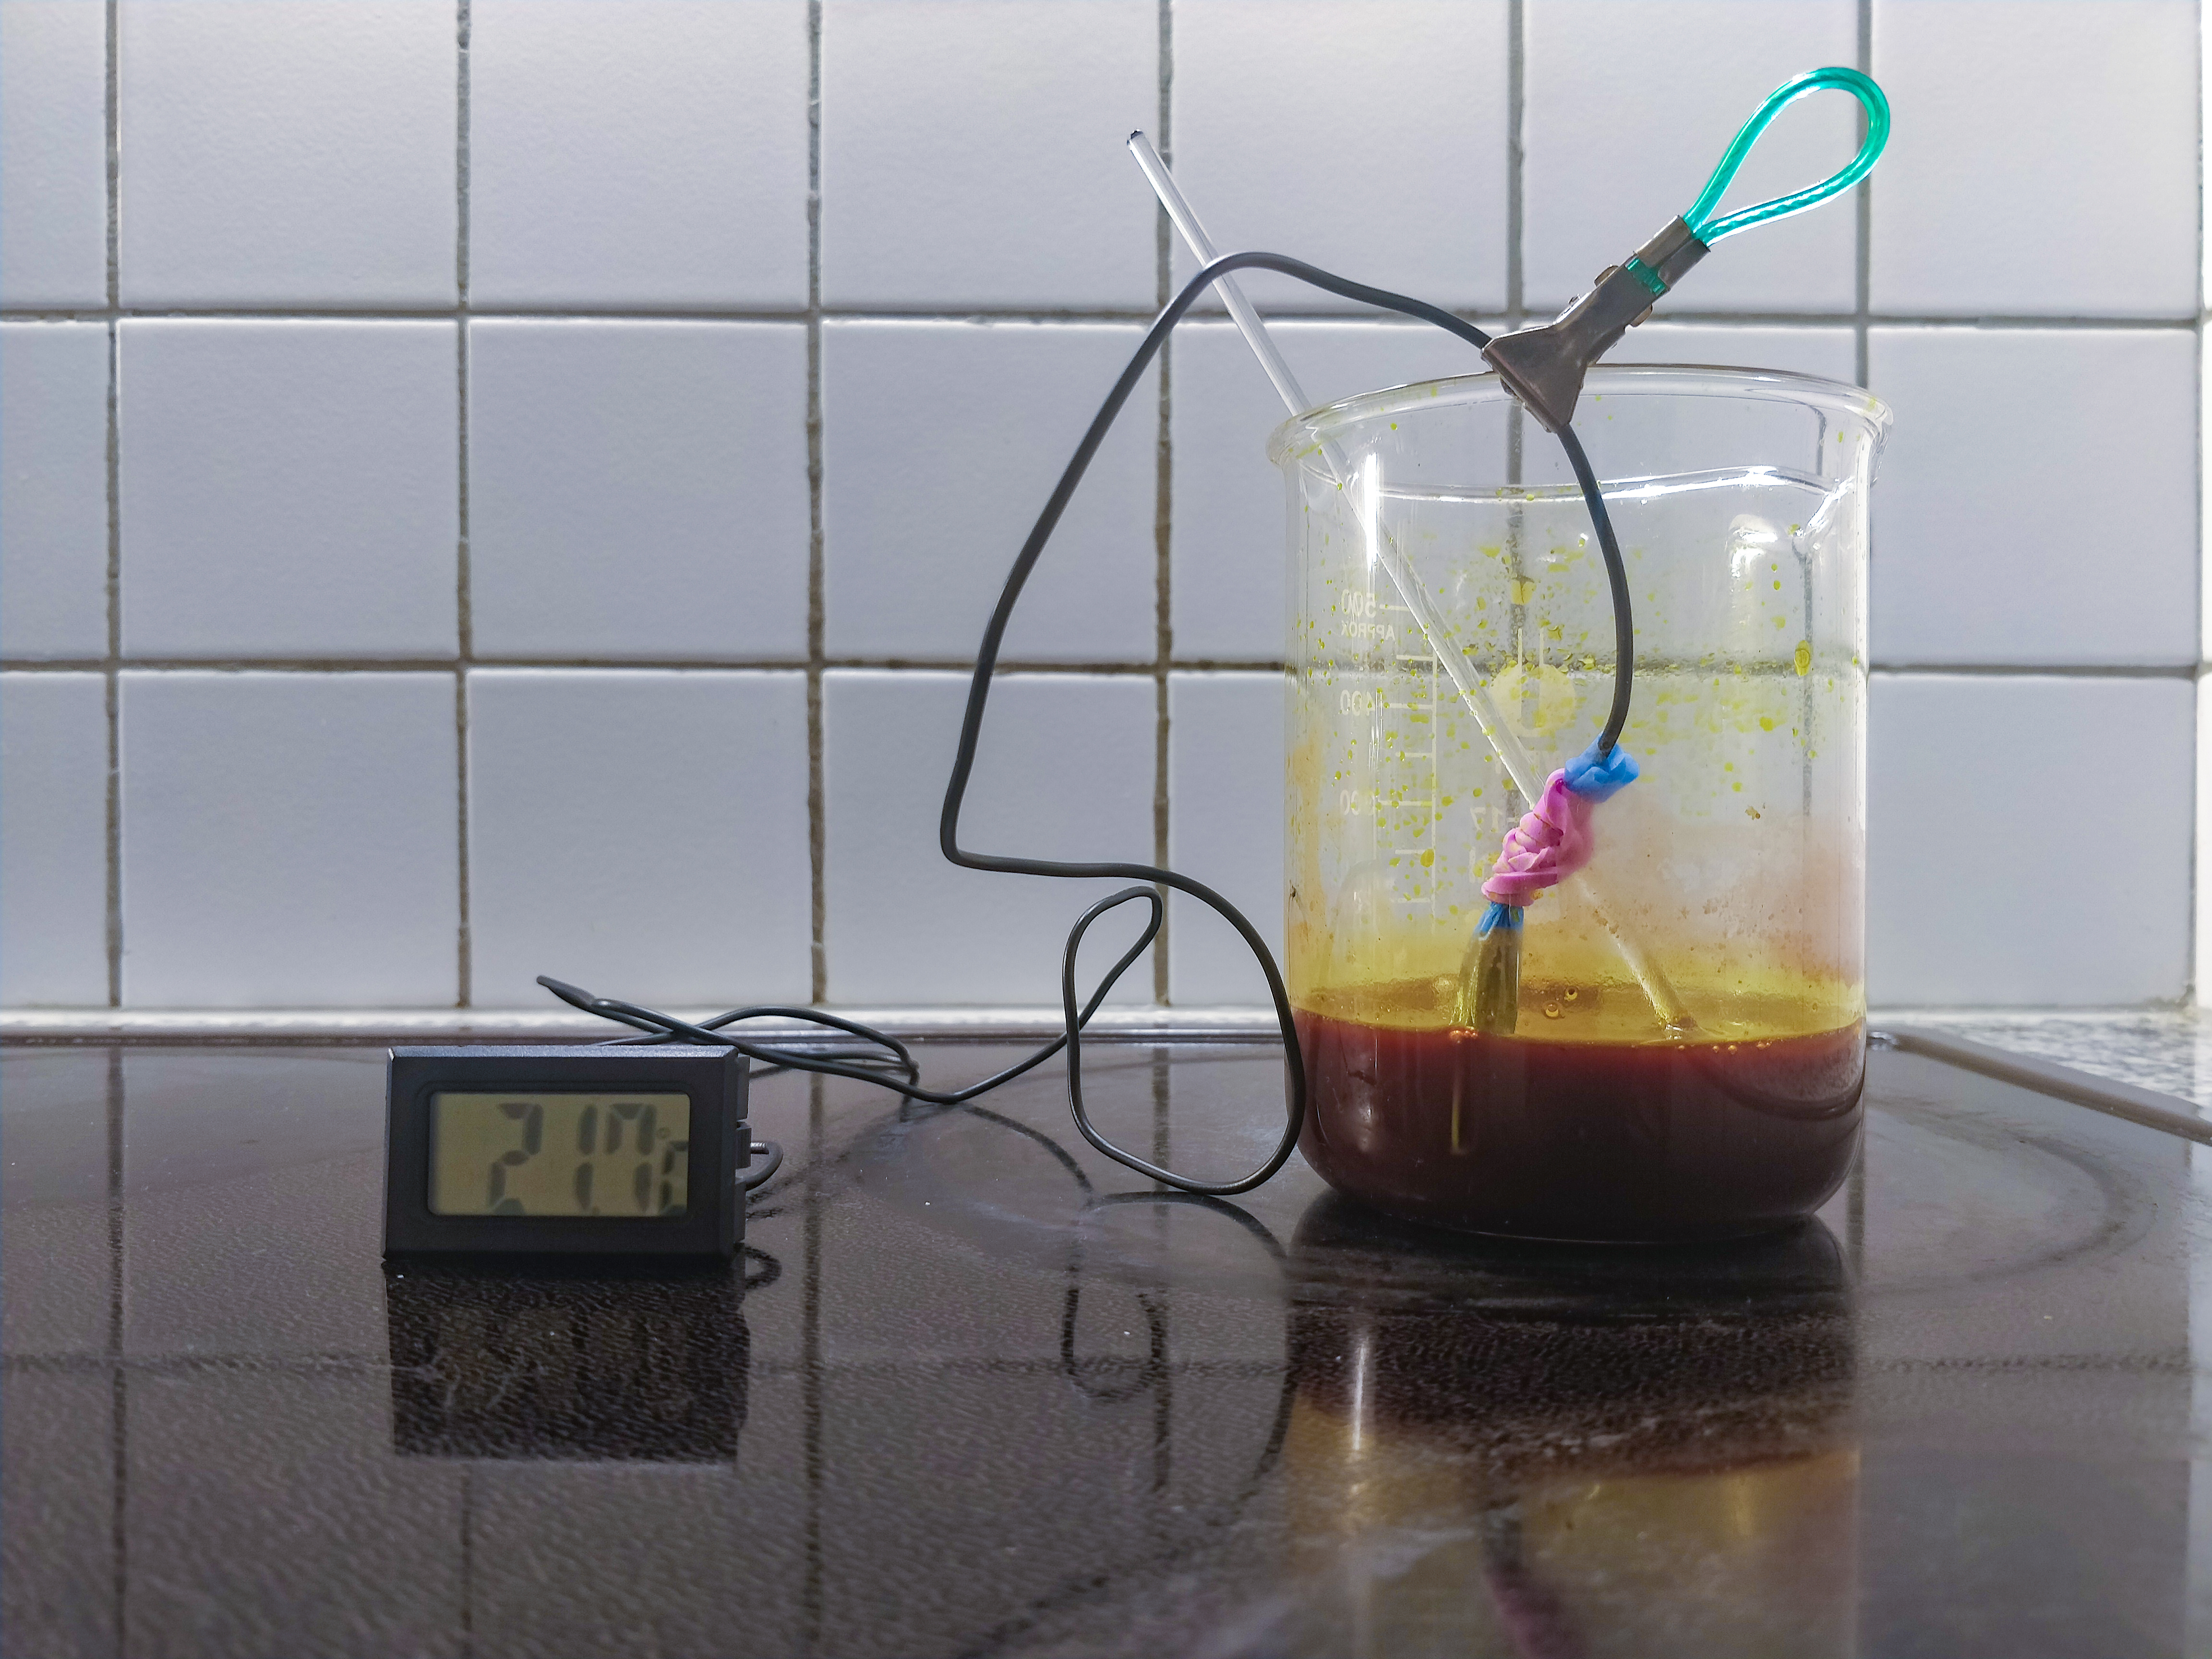
\includegraphics[width=\linewidth]{media/album/PSX_20220301_014813.jpg}
            \caption{}
            \label{fig:PhotoSolution}
        \end{minipage}
    \end{figure}


    Il processo consiste della tecnica di tutte le schede DIY\footnote{Do-It-Yourself, o fai-da-te}, come gi\`{a} detto,occorre stampare il circuito su un pezzo di carta, posarlo con la parte colorata sulla superficie pulita della scheda preparata e attaccare il toner per via dell'applicazione temporanea del calore\footnote{Normalmente si usa un ferro da stiro}\:\footnote{Figura \ref{fig:PhotoPCBIron}}.
    Poi il foglio con il circuito deve essere tolto\footnote{Figura\ref{fig:PhotoPCBWash}} con cautela.
    Il metodo pi\`{u} efficace \`{e} il bagnare il foglio e consumarlo a poco a poco con qualcosa di ruvido, ma soffice come una spugna.
    Avendo pulito totalmente il circuito mi sono ritrovato delle tracce di toner attaccate alla superficie della scheda.
    Coloro saranno da protezione dalla soluzione per l'incisione chimica: le parti scoperte reagiranno con la soluzione consumandosi con l'andare del tempo, mentre le parti coperte rimarranno attaccate.

    \begin{figure}[H]
        \centering
        \begin{minipage}[H]{.331\linewidth}
            \centering
            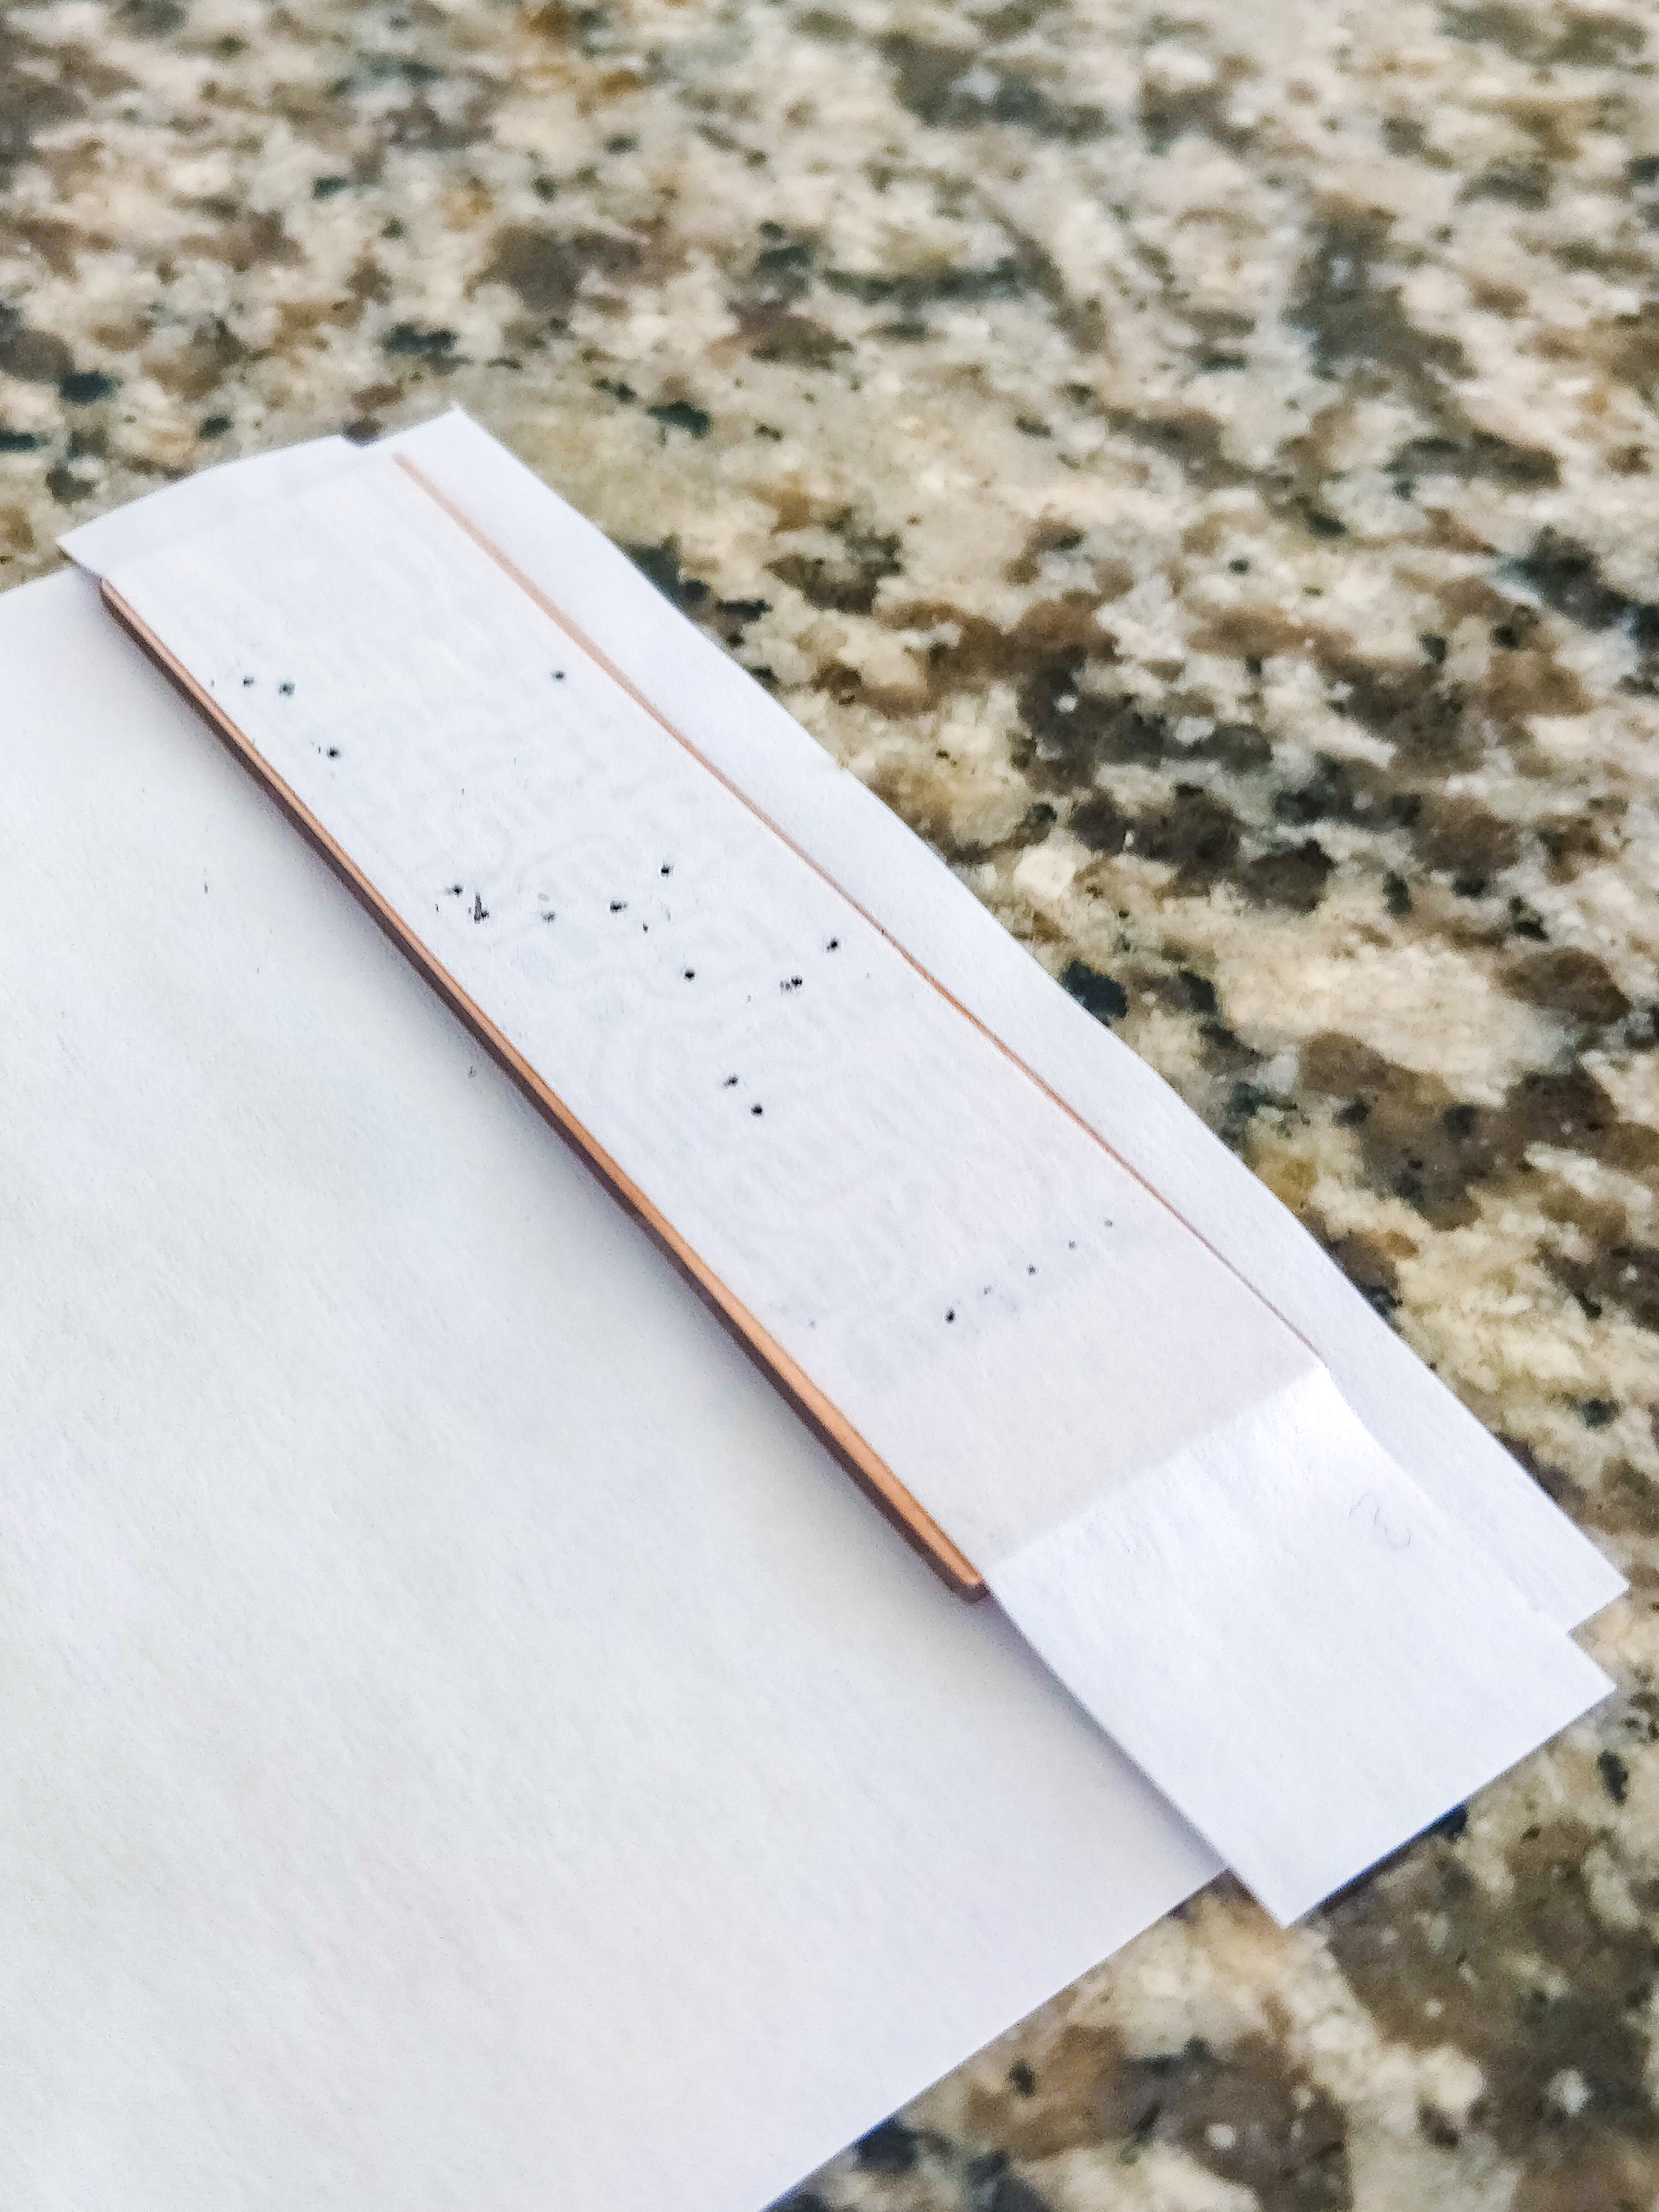
\includegraphics[width=\linewidth]{media/album/PSX_20220228_020336.jpg}
            \caption{}
            \label{fig:PhotoPCBIron}
        \end{minipage}
        \hspace{.04\linewidth}
        \begin{minipage}[H]{.5888\linewidth}
            \centering
            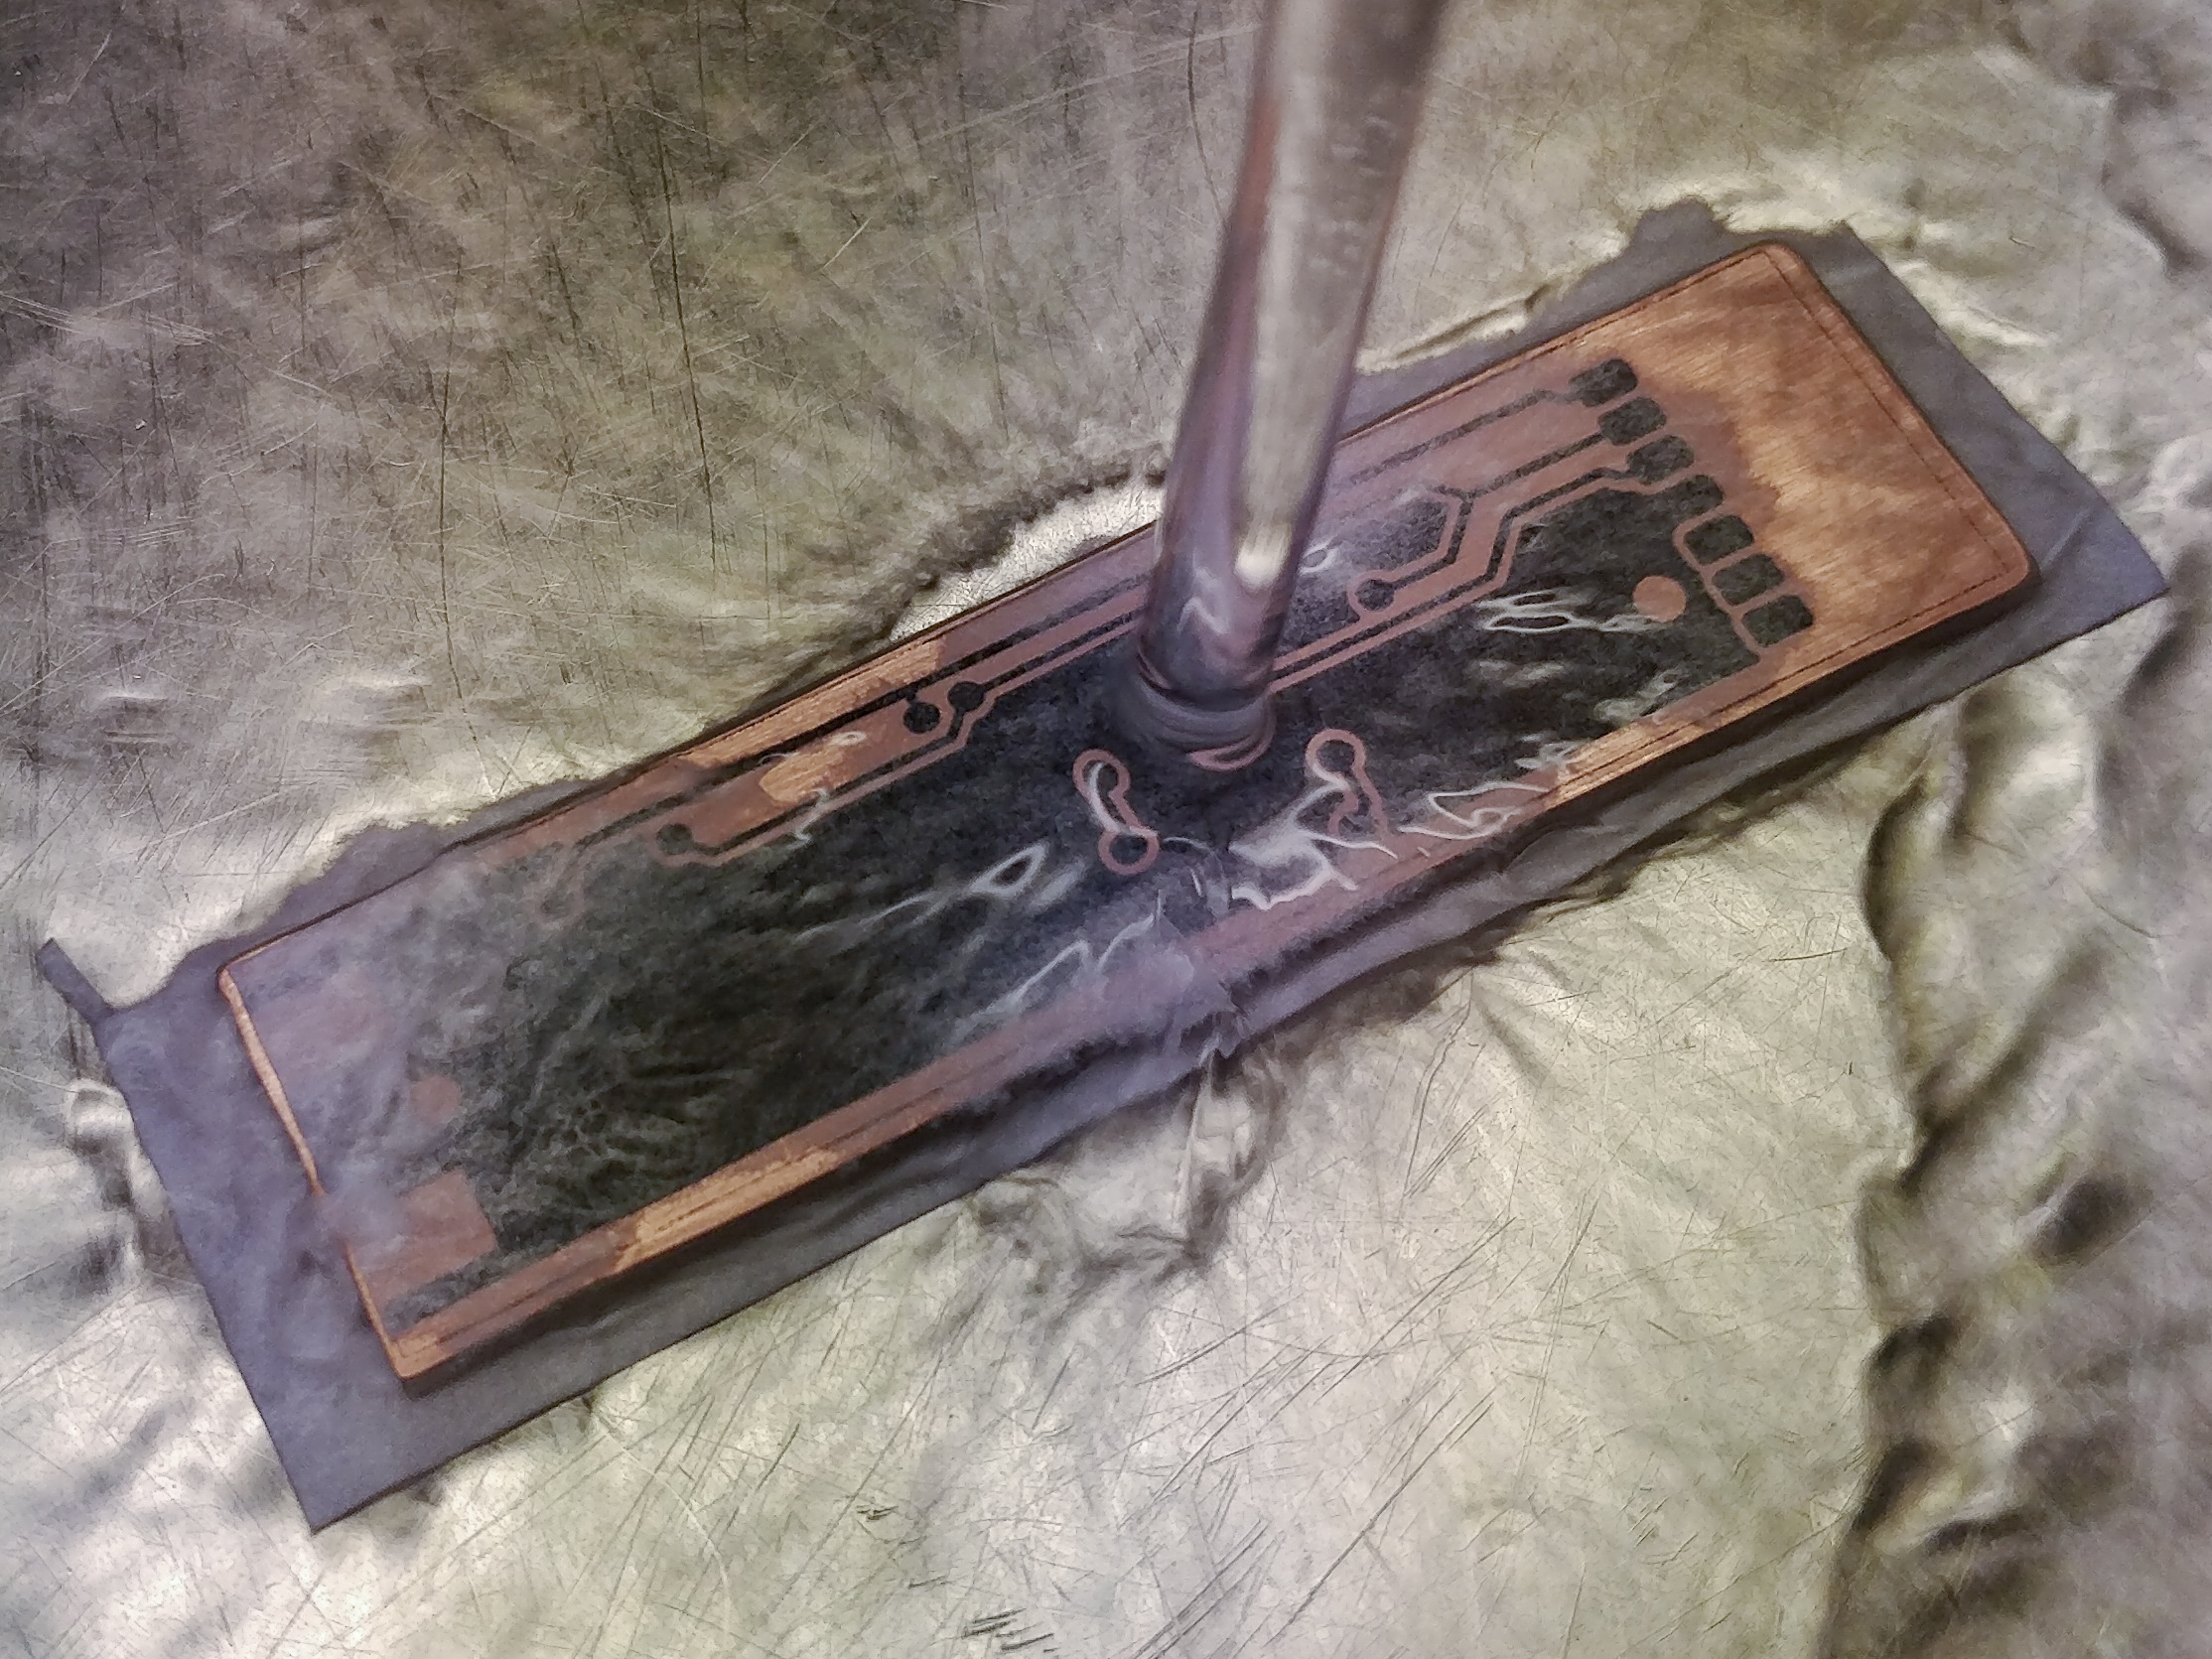
\includegraphics[width=\linewidth]{media/album/PSX_20220301_034705.jpg}
            \caption{}
            \label{fig:PhotoPCBWash}
        \end{minipage}
    \end{figure}
    \clearpage

    In un lasso di 10 minuti il circuito \`{e} rimasto\footnote{Figure \ref{fig:PhotoPCBPrepare1}, \ref{fig:PhotoPCBPrepare2}, \ref{fig:PhotoPCBPrepare3}, \ref{fig:PhotoPCBPrepareDone}} nella soluzione, mentre il rame si dissolveva a poco a poco.
    Inoltre la soluzione pu\`{o} essere scaldata un po'per velocizzare il processo \emph{(Sempre senza superare i $55^{\circ}C$)}
    \begin{figure}[H]
        \centering
        \begin{minipage}[H]{.45\linewidth}
            \centering
            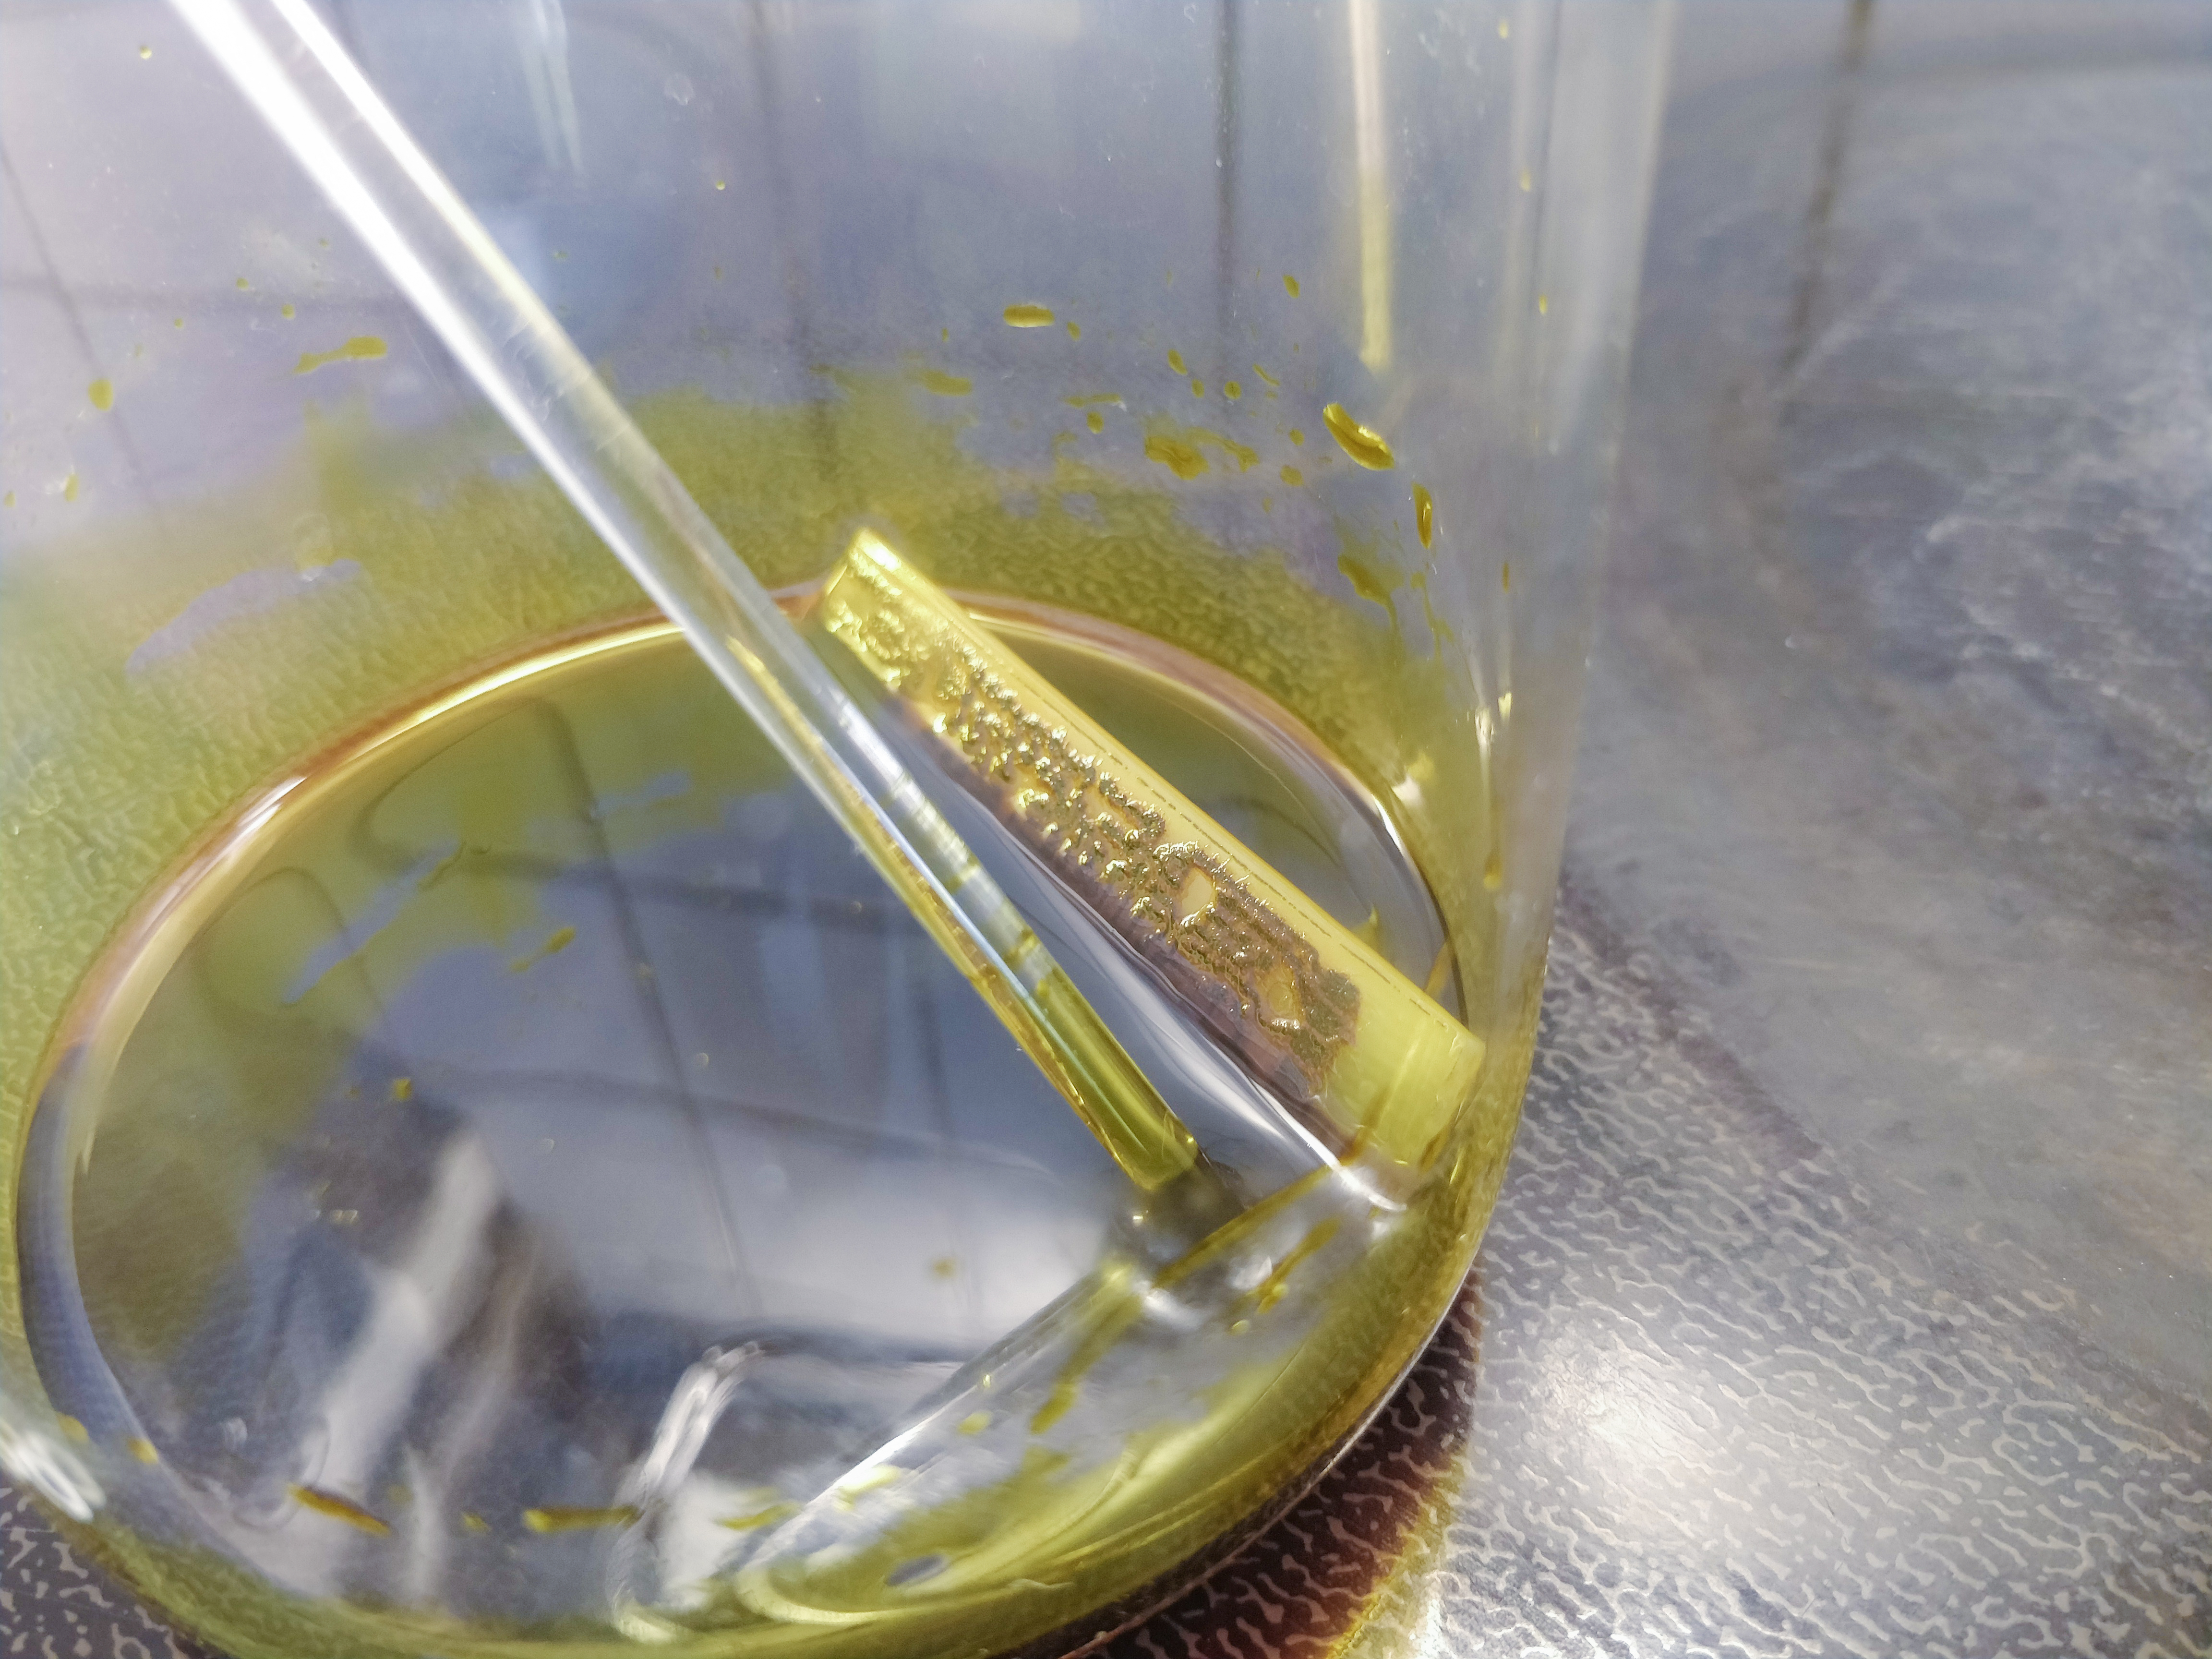
\includegraphics[width=\linewidth]{media/album/PSX_20220301_014718.jpg}
            \caption{}
            \label{fig:PhotoPCBPrepare1}
        \end{minipage}
        \hspace{.04\linewidth}
        \begin{minipage}[H]{.45\linewidth}
            \centering
            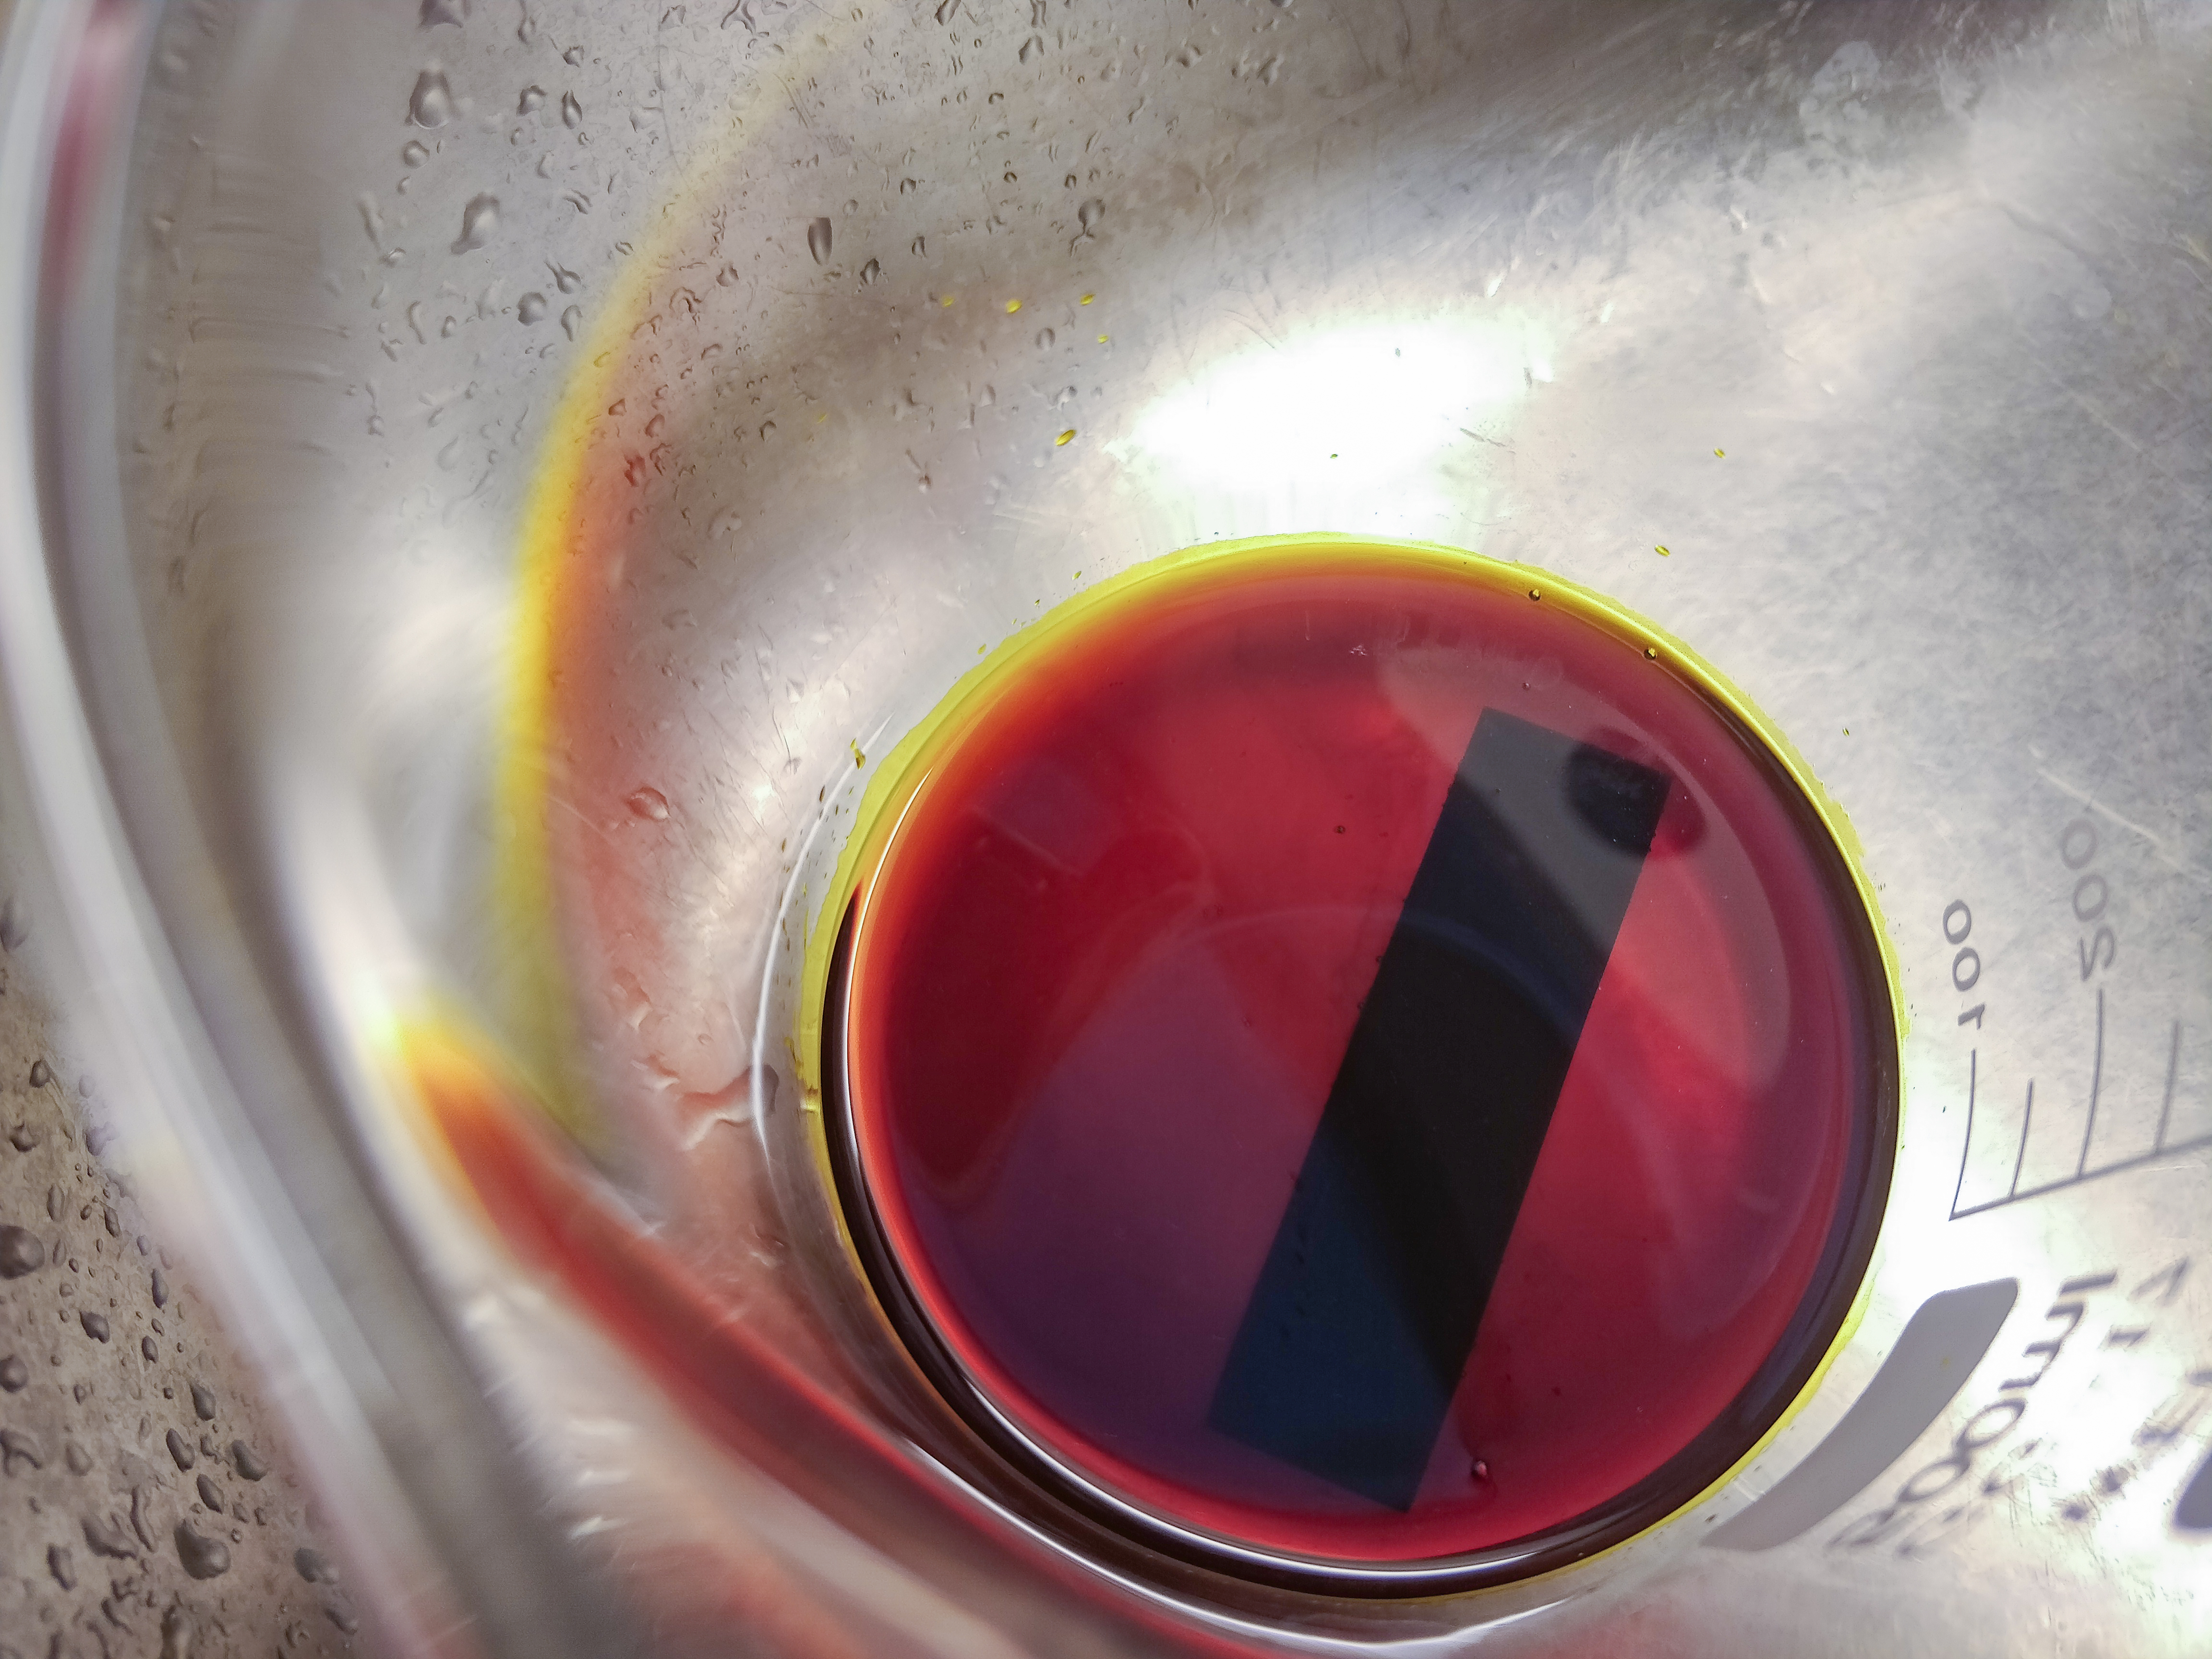
\includegraphics[width=\linewidth]{media/album/PSX_20220301_014557.jpg}
            \caption{}
            \label{fig:PhotoPCBPrepare2}
        \end{minipage}
        \\
        \vspace*{.01\linewidth}
        \begin{minipage}[H]{.95\linewidth}
            \centering
            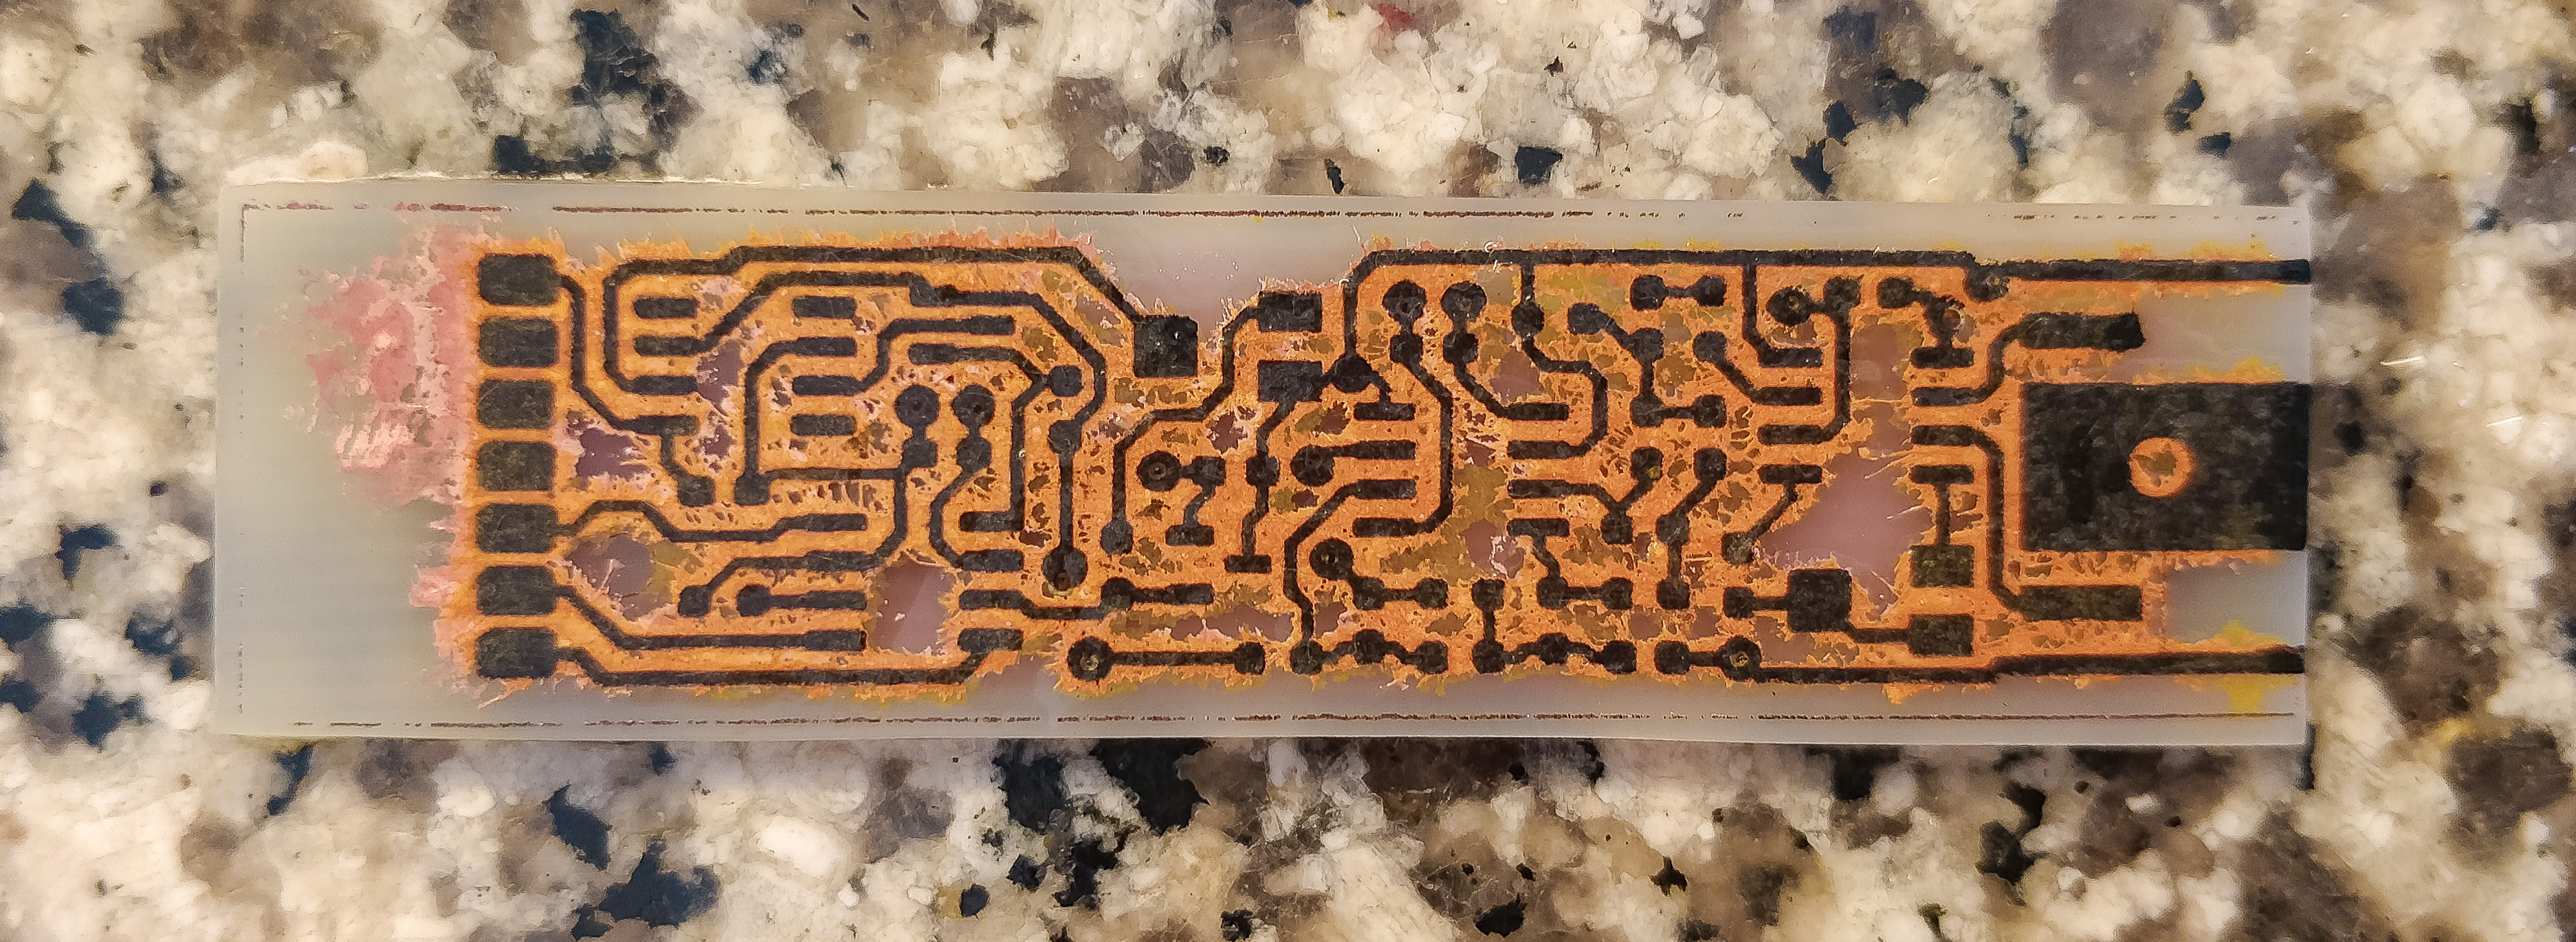
\includegraphics[width=\linewidth]{media/album/PSX_20220228_015716.jpg}
            \caption{}
            \label{fig:PhotoPCBPrepare3}
        \end{minipage}
        \\
        \vspace*{.01\linewidth}
        \begin{minipage}[H]{.95\linewidth}
            \centering
            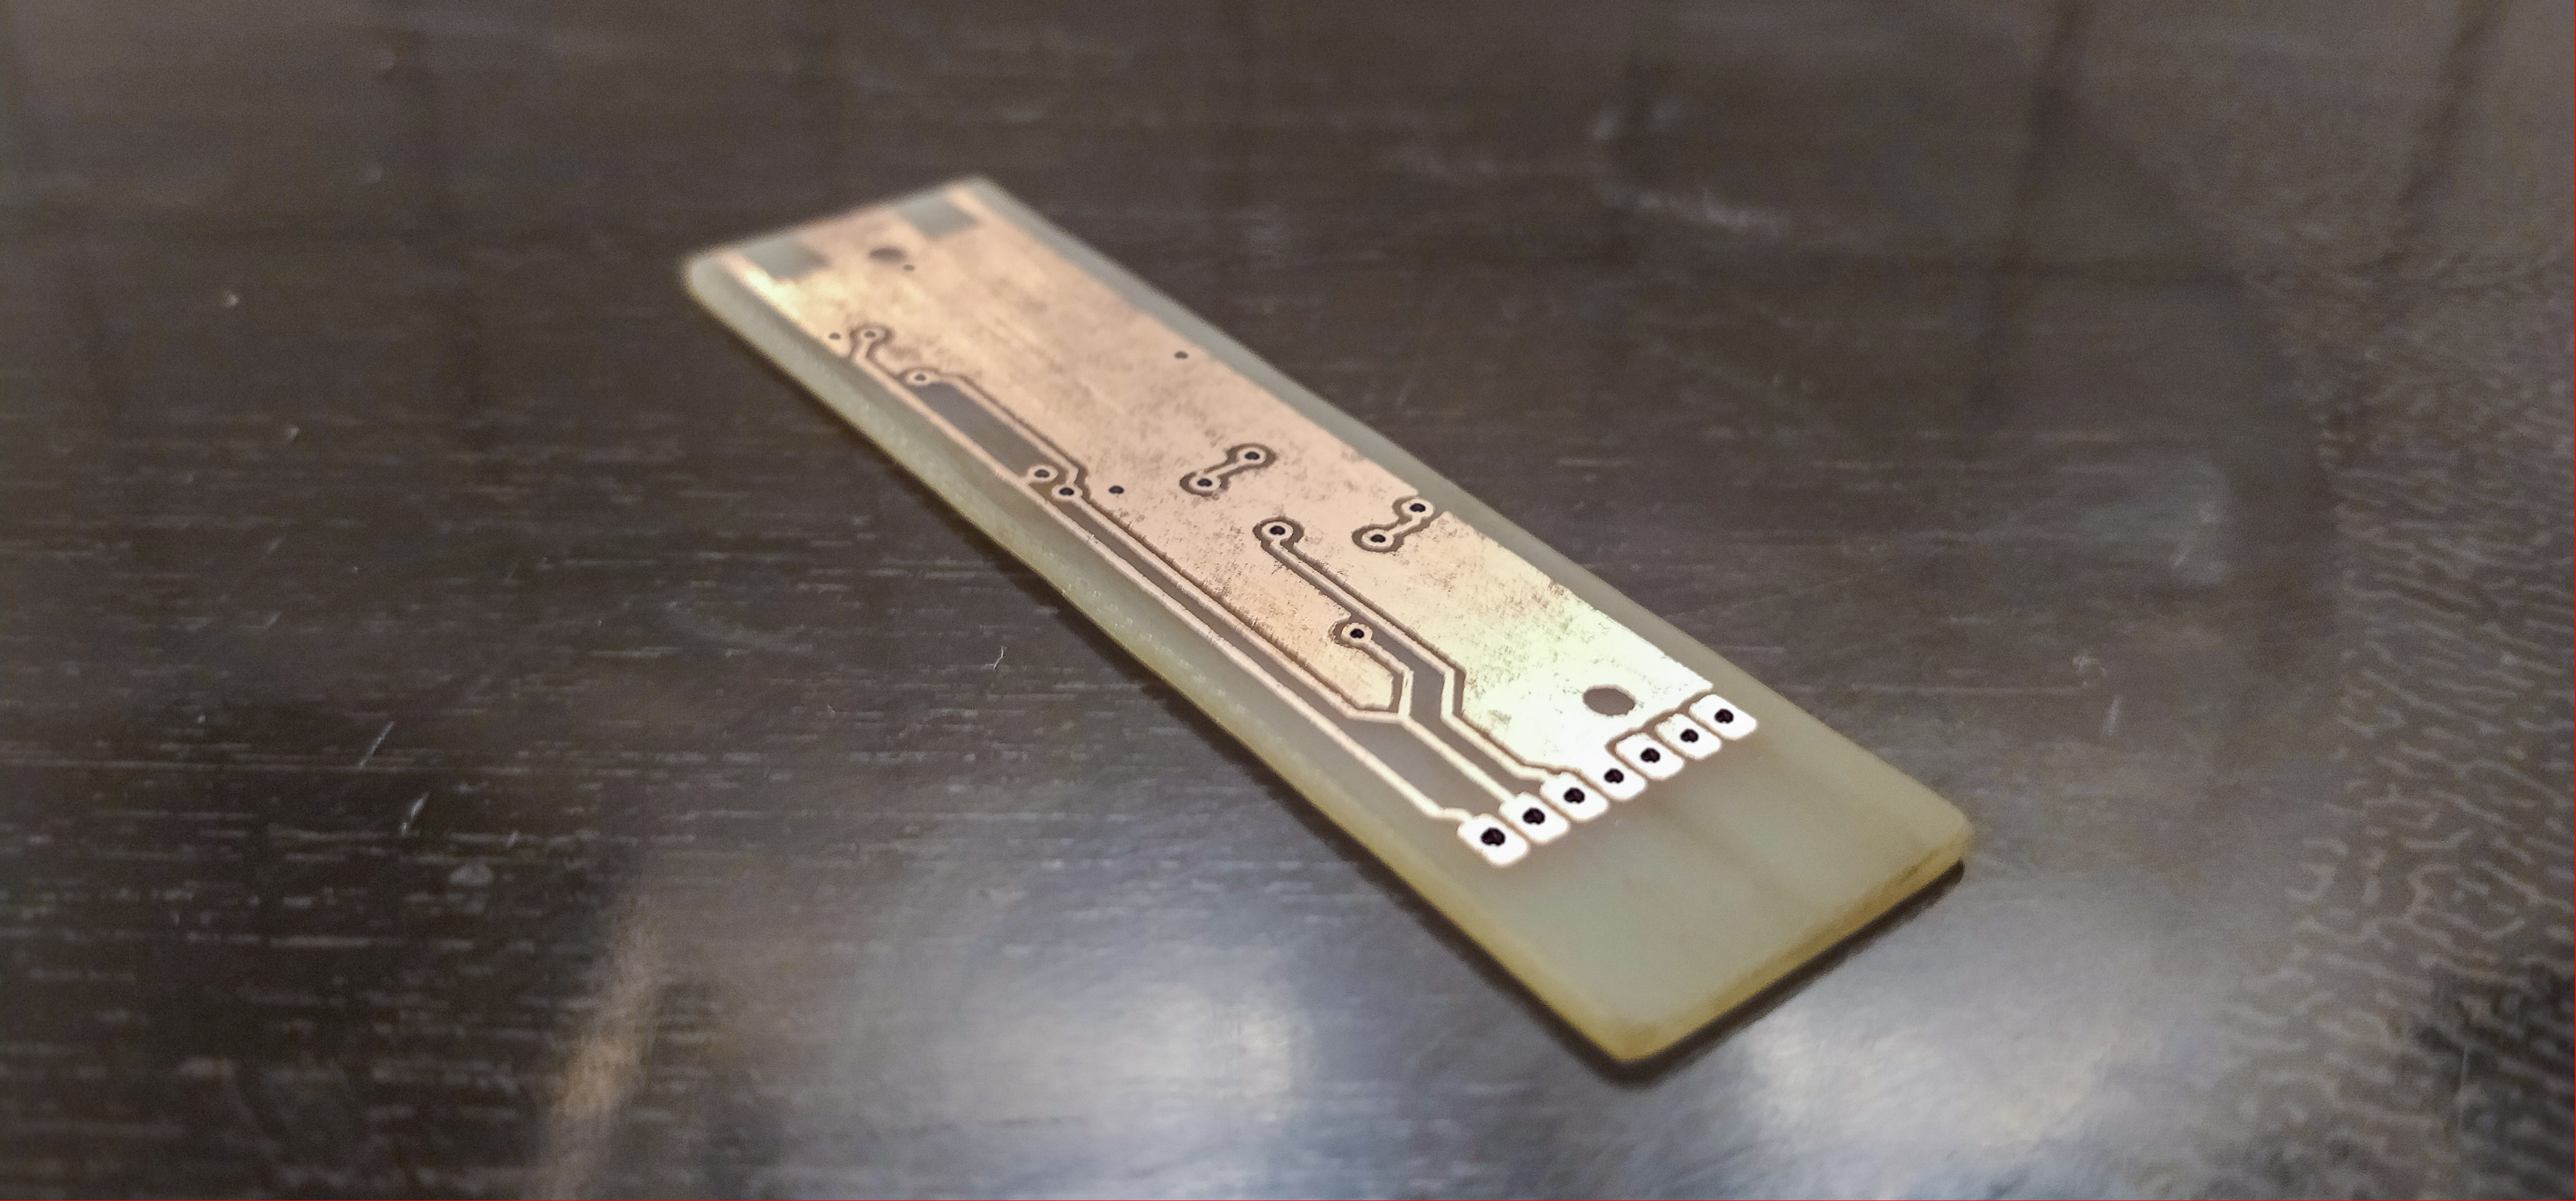
\includegraphics[width=\linewidth]{media/album/PSX_20220301_054445.jpg}
            \caption{}
            \label{fig:PhotoPCBPrepareDone}
        \end{minipage}
    \end{figure}

    La prossima tappa \`{e} quella di saldare\footnote{Figure \ref{fig:PhotoPCBProgress1}, \ref{fig:PhotoPCBProgress2}, \ref{fig:PhotoPCBProgress3}, \ref{fig:PhotoCableProgress4}, \ref{fig:PhotoCableProgress5}} il circuito e qui entrano in atto le abilit\`{a} micromotorie.
    Gli unici consigli che posso dare, sono di fare attenzione all'antiossidante che si usa, per il motivo che alcuni conducono elettricit\`{a} e se non tolti interamente\footnote{Con i componenti di formato SMD non si riesce a togliere dal sotto dell'elemento che si salda} dopo la saldatura, possono causare malfunzionamenti.
    \begin{figure}[H]
        \centering
        \begin{minipage}[H]{.45\linewidth}
            \centering
            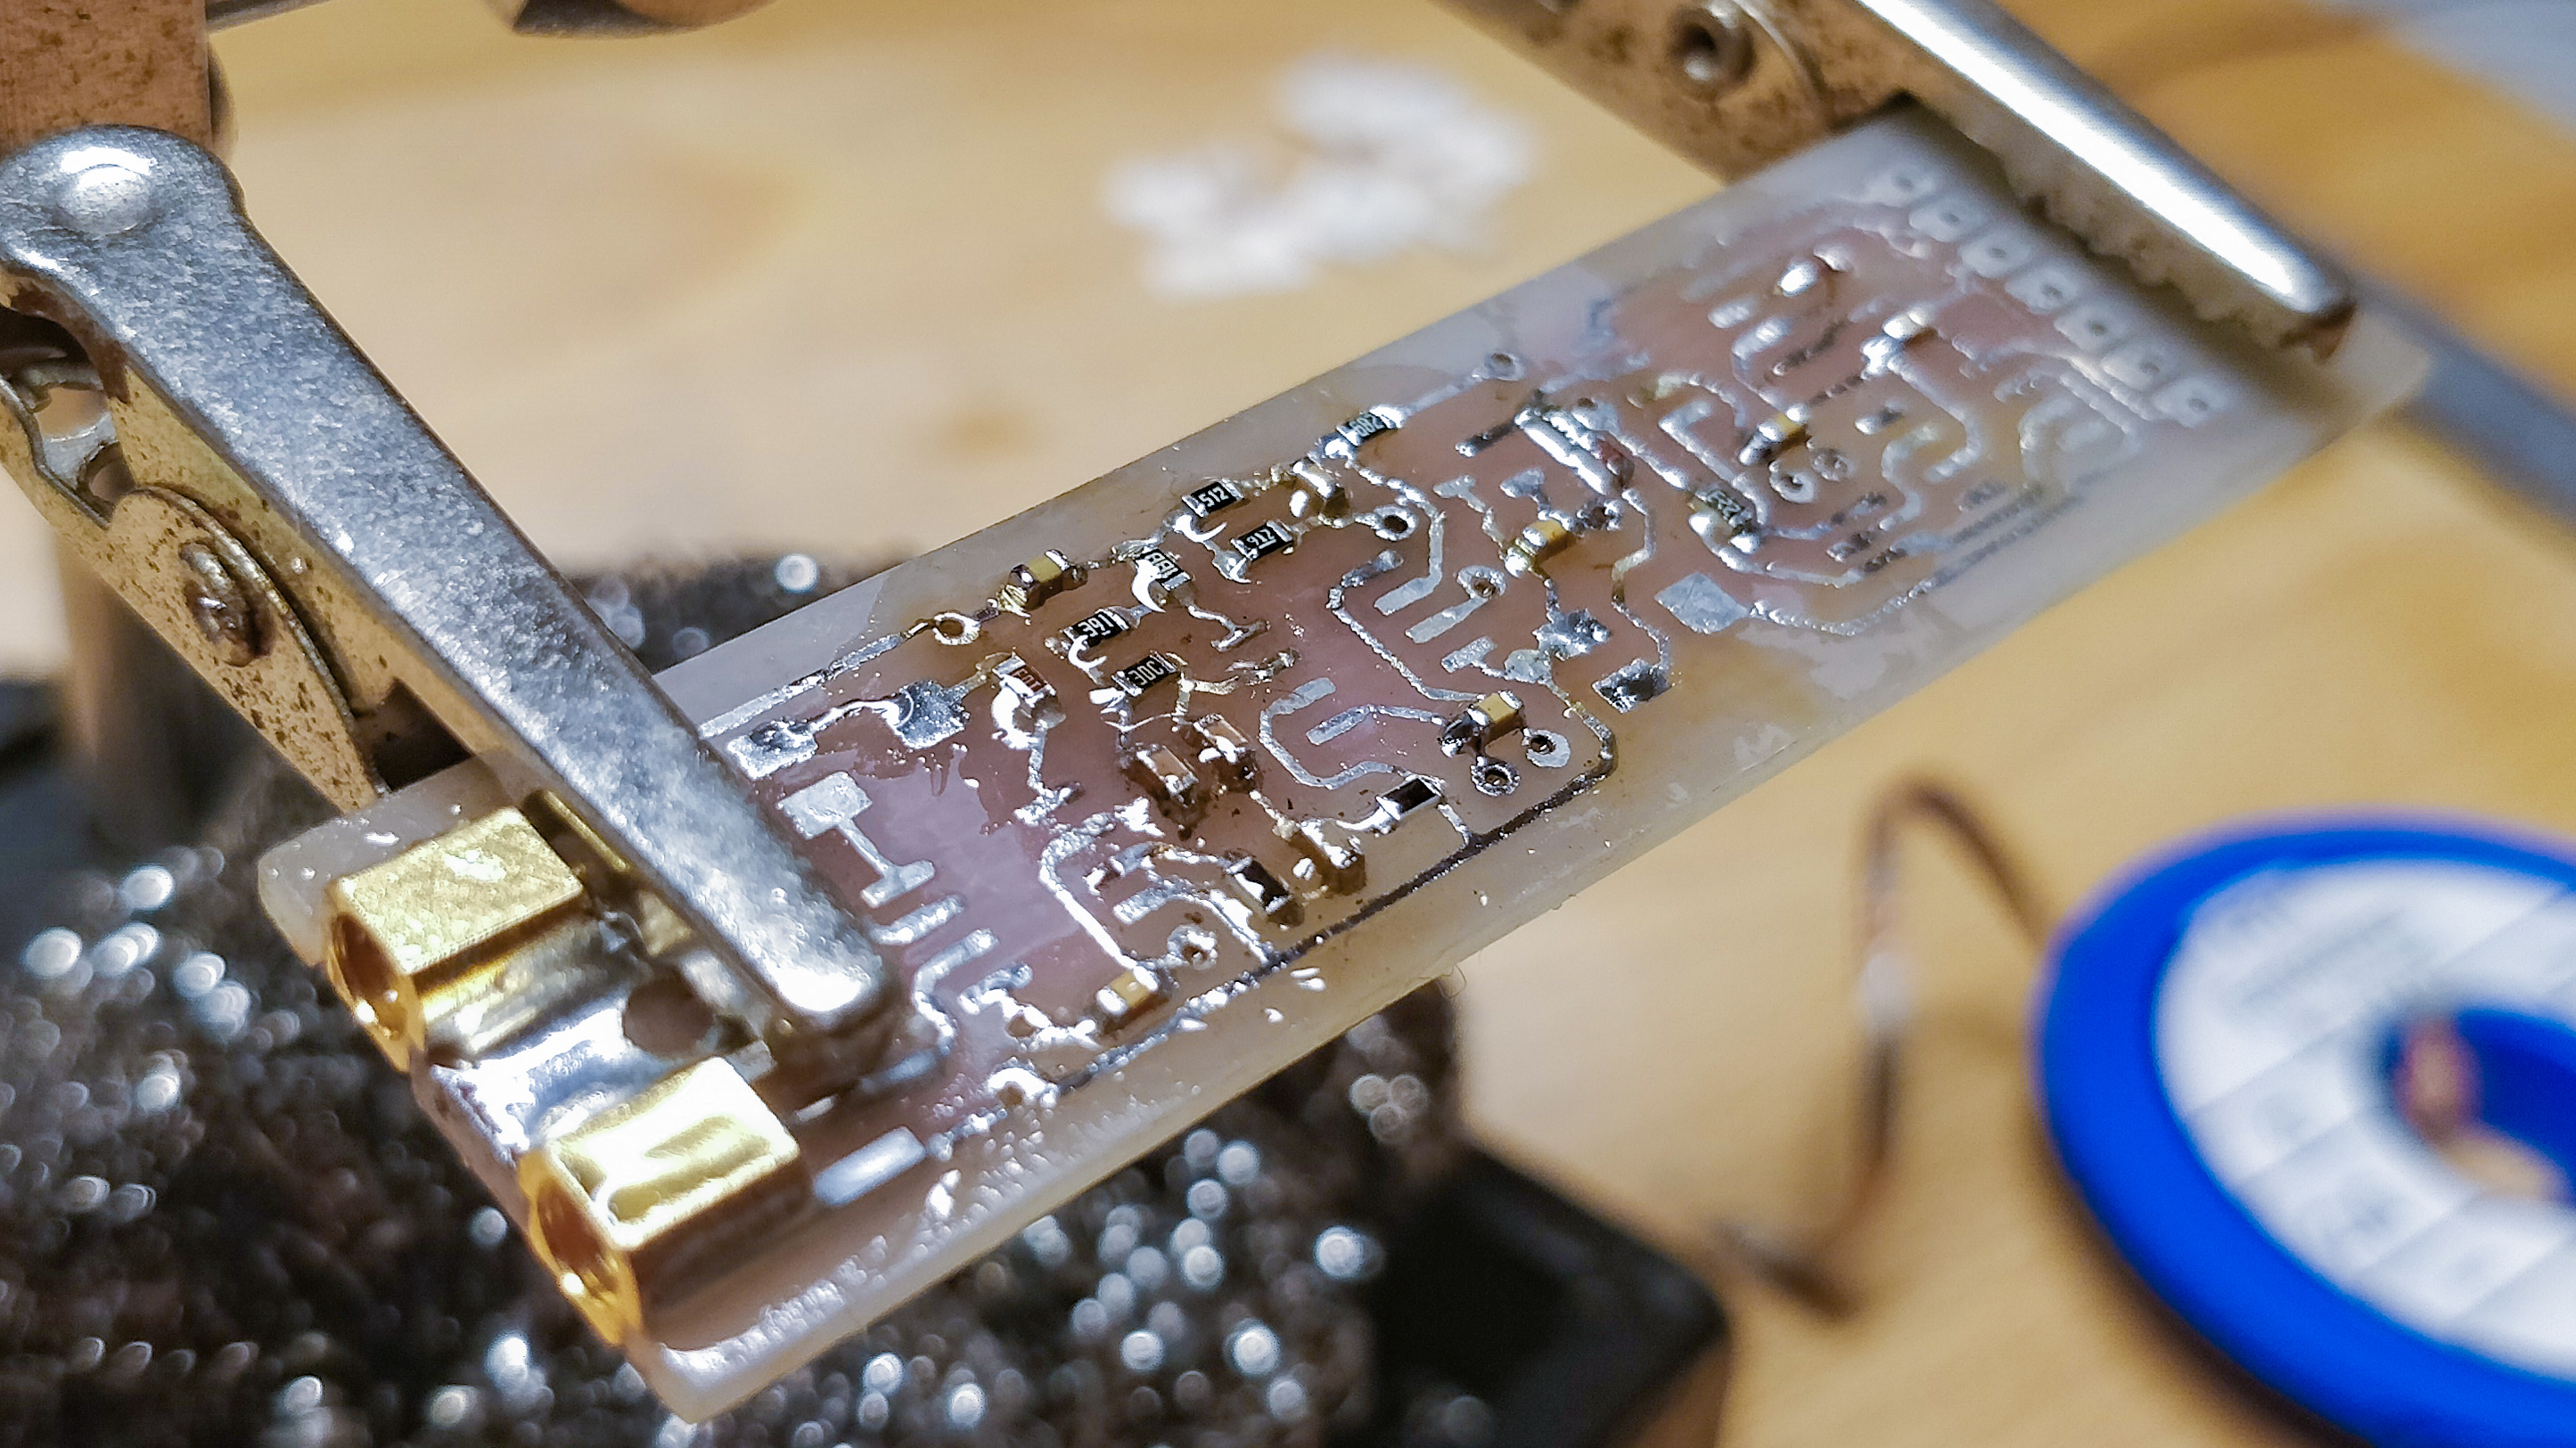
\includegraphics[width=\linewidth]{media/album/PSX_20220228_161847.jpg}
            \caption{}
            \label{fig:PhotoPCBProgress1}
        \end{minipage}
        \hspace{.04\linewidth}
        \begin{minipage}[H]{.45\linewidth}
            \centering
            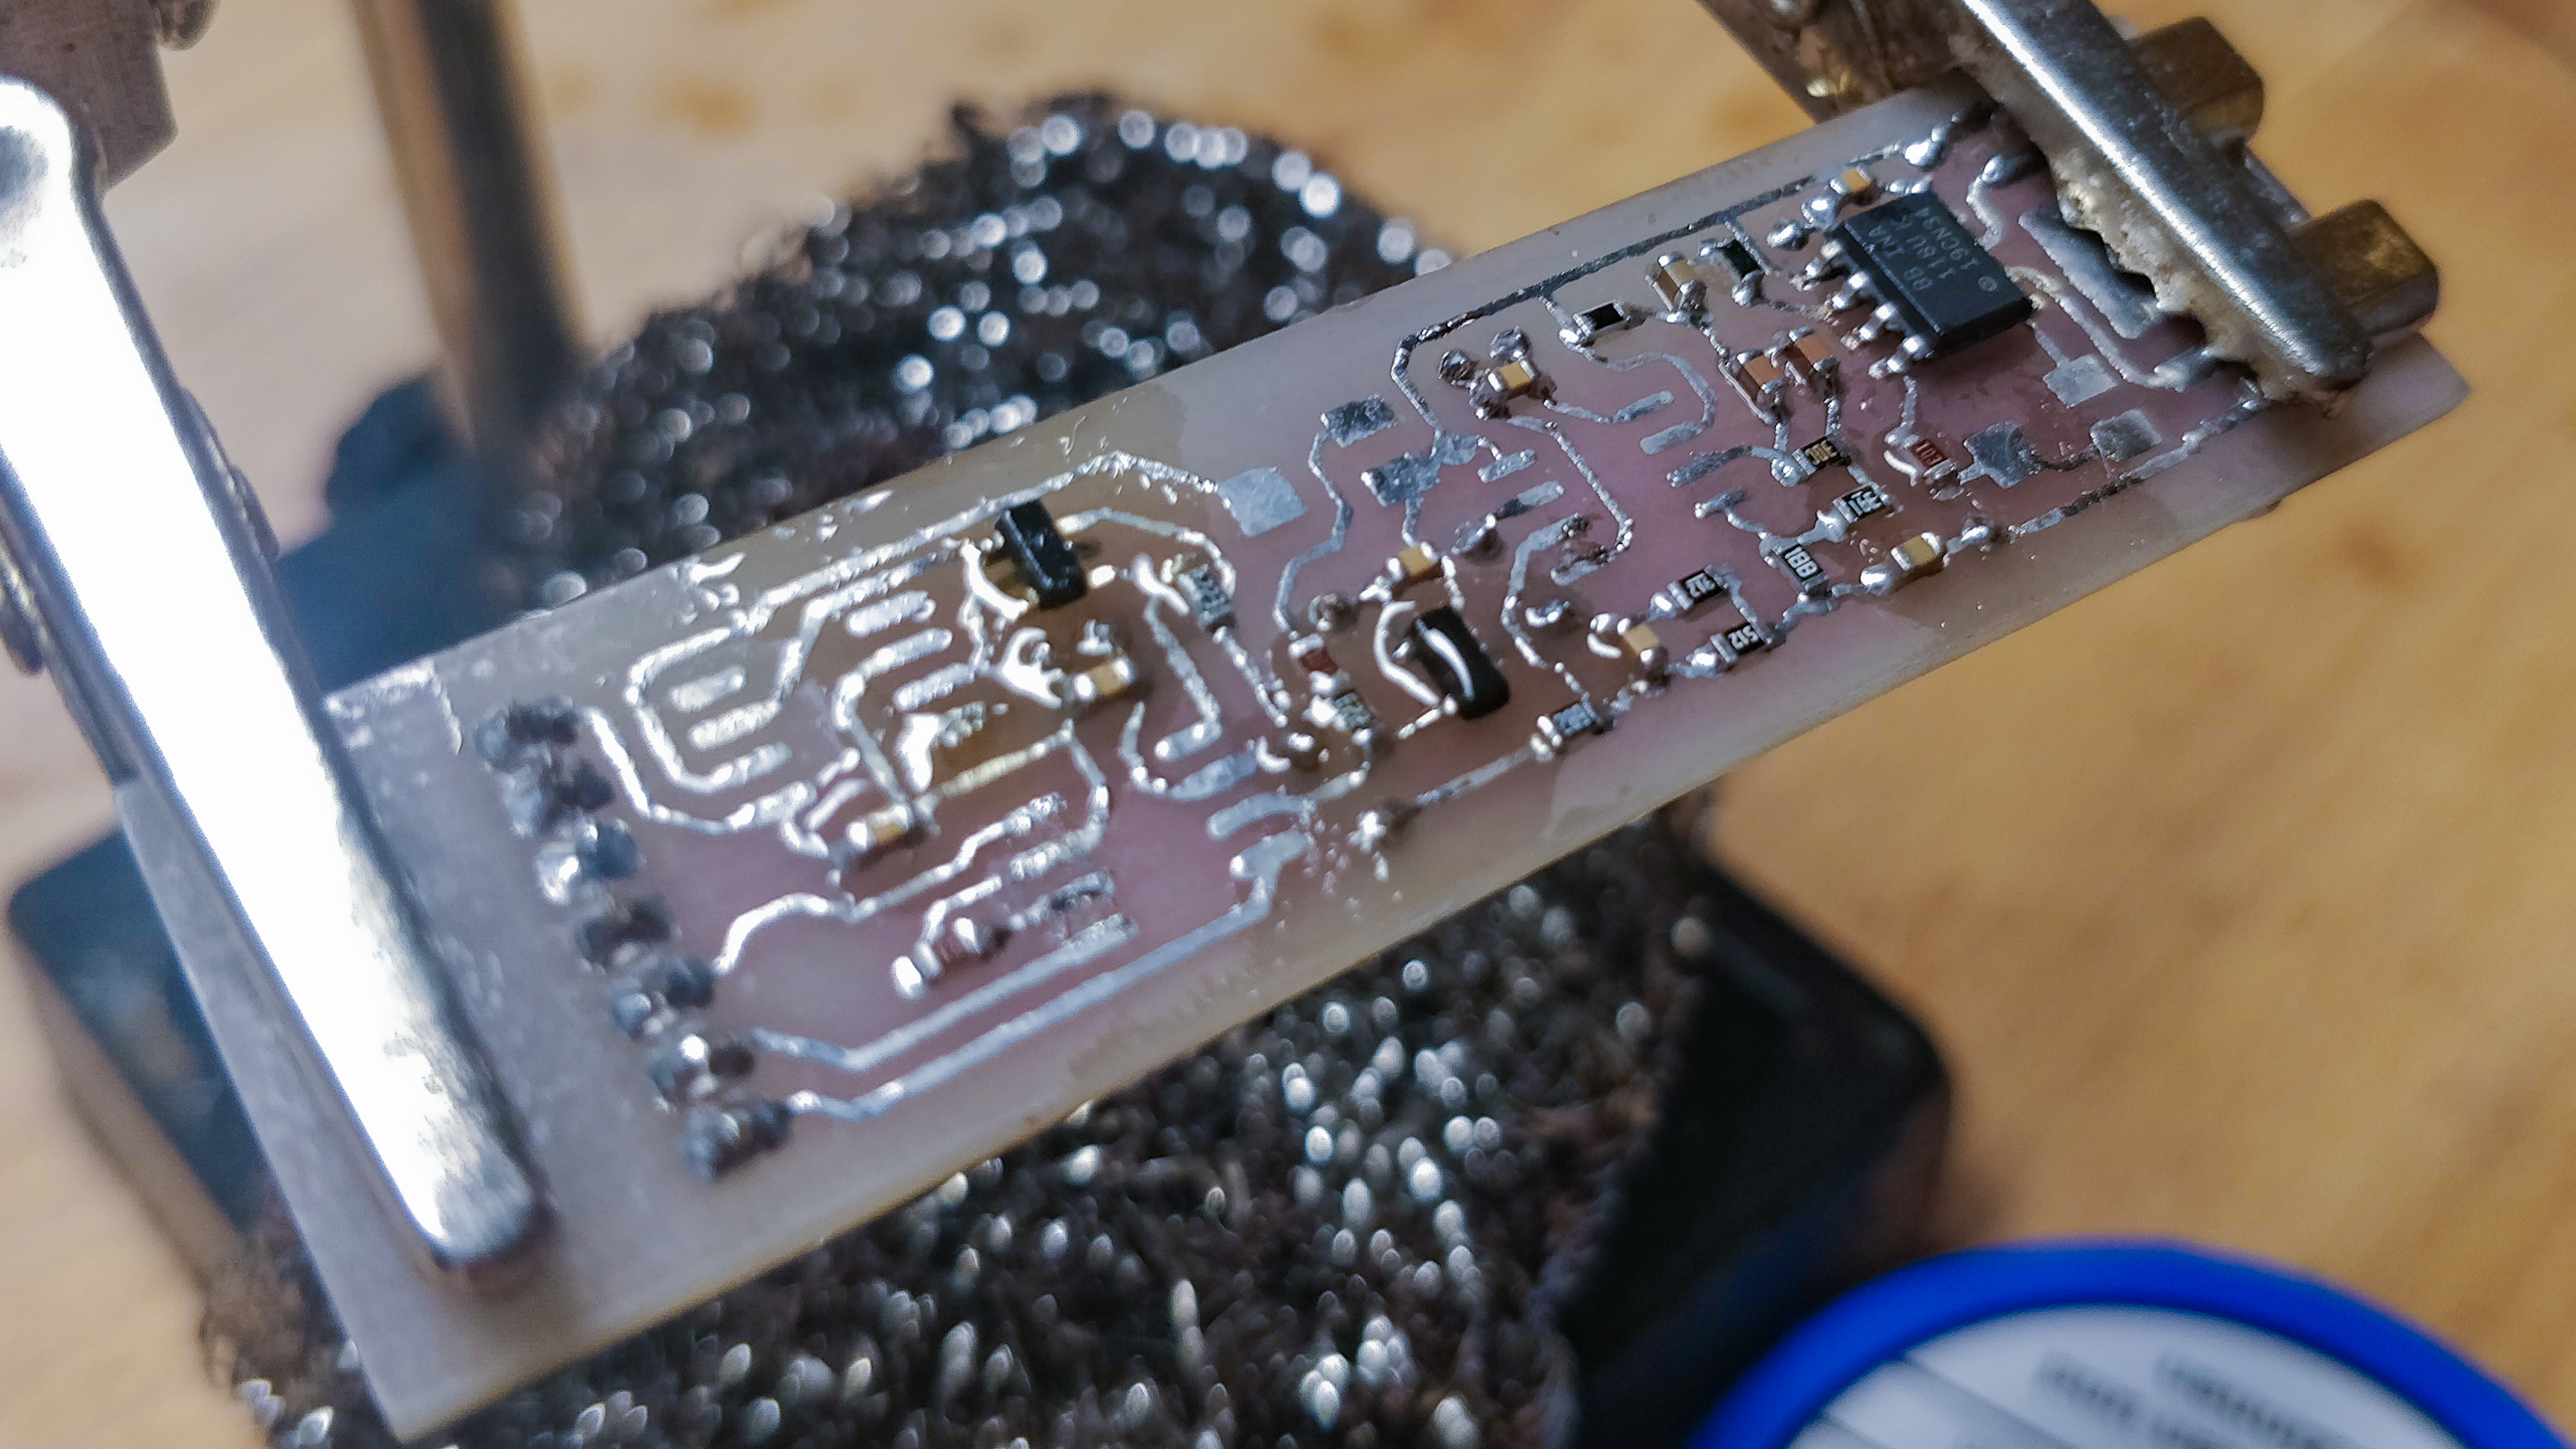
\includegraphics[width=\linewidth]{media/album/PSX_20220228_162014.jpg}
            \caption{}
            \label{fig:PhotoPCBProgress2}
        \end{minipage}
        \\
        \vspace*{.01\linewidth}
        \begin{minipage}[H]{.95\linewidth}
            \centering
            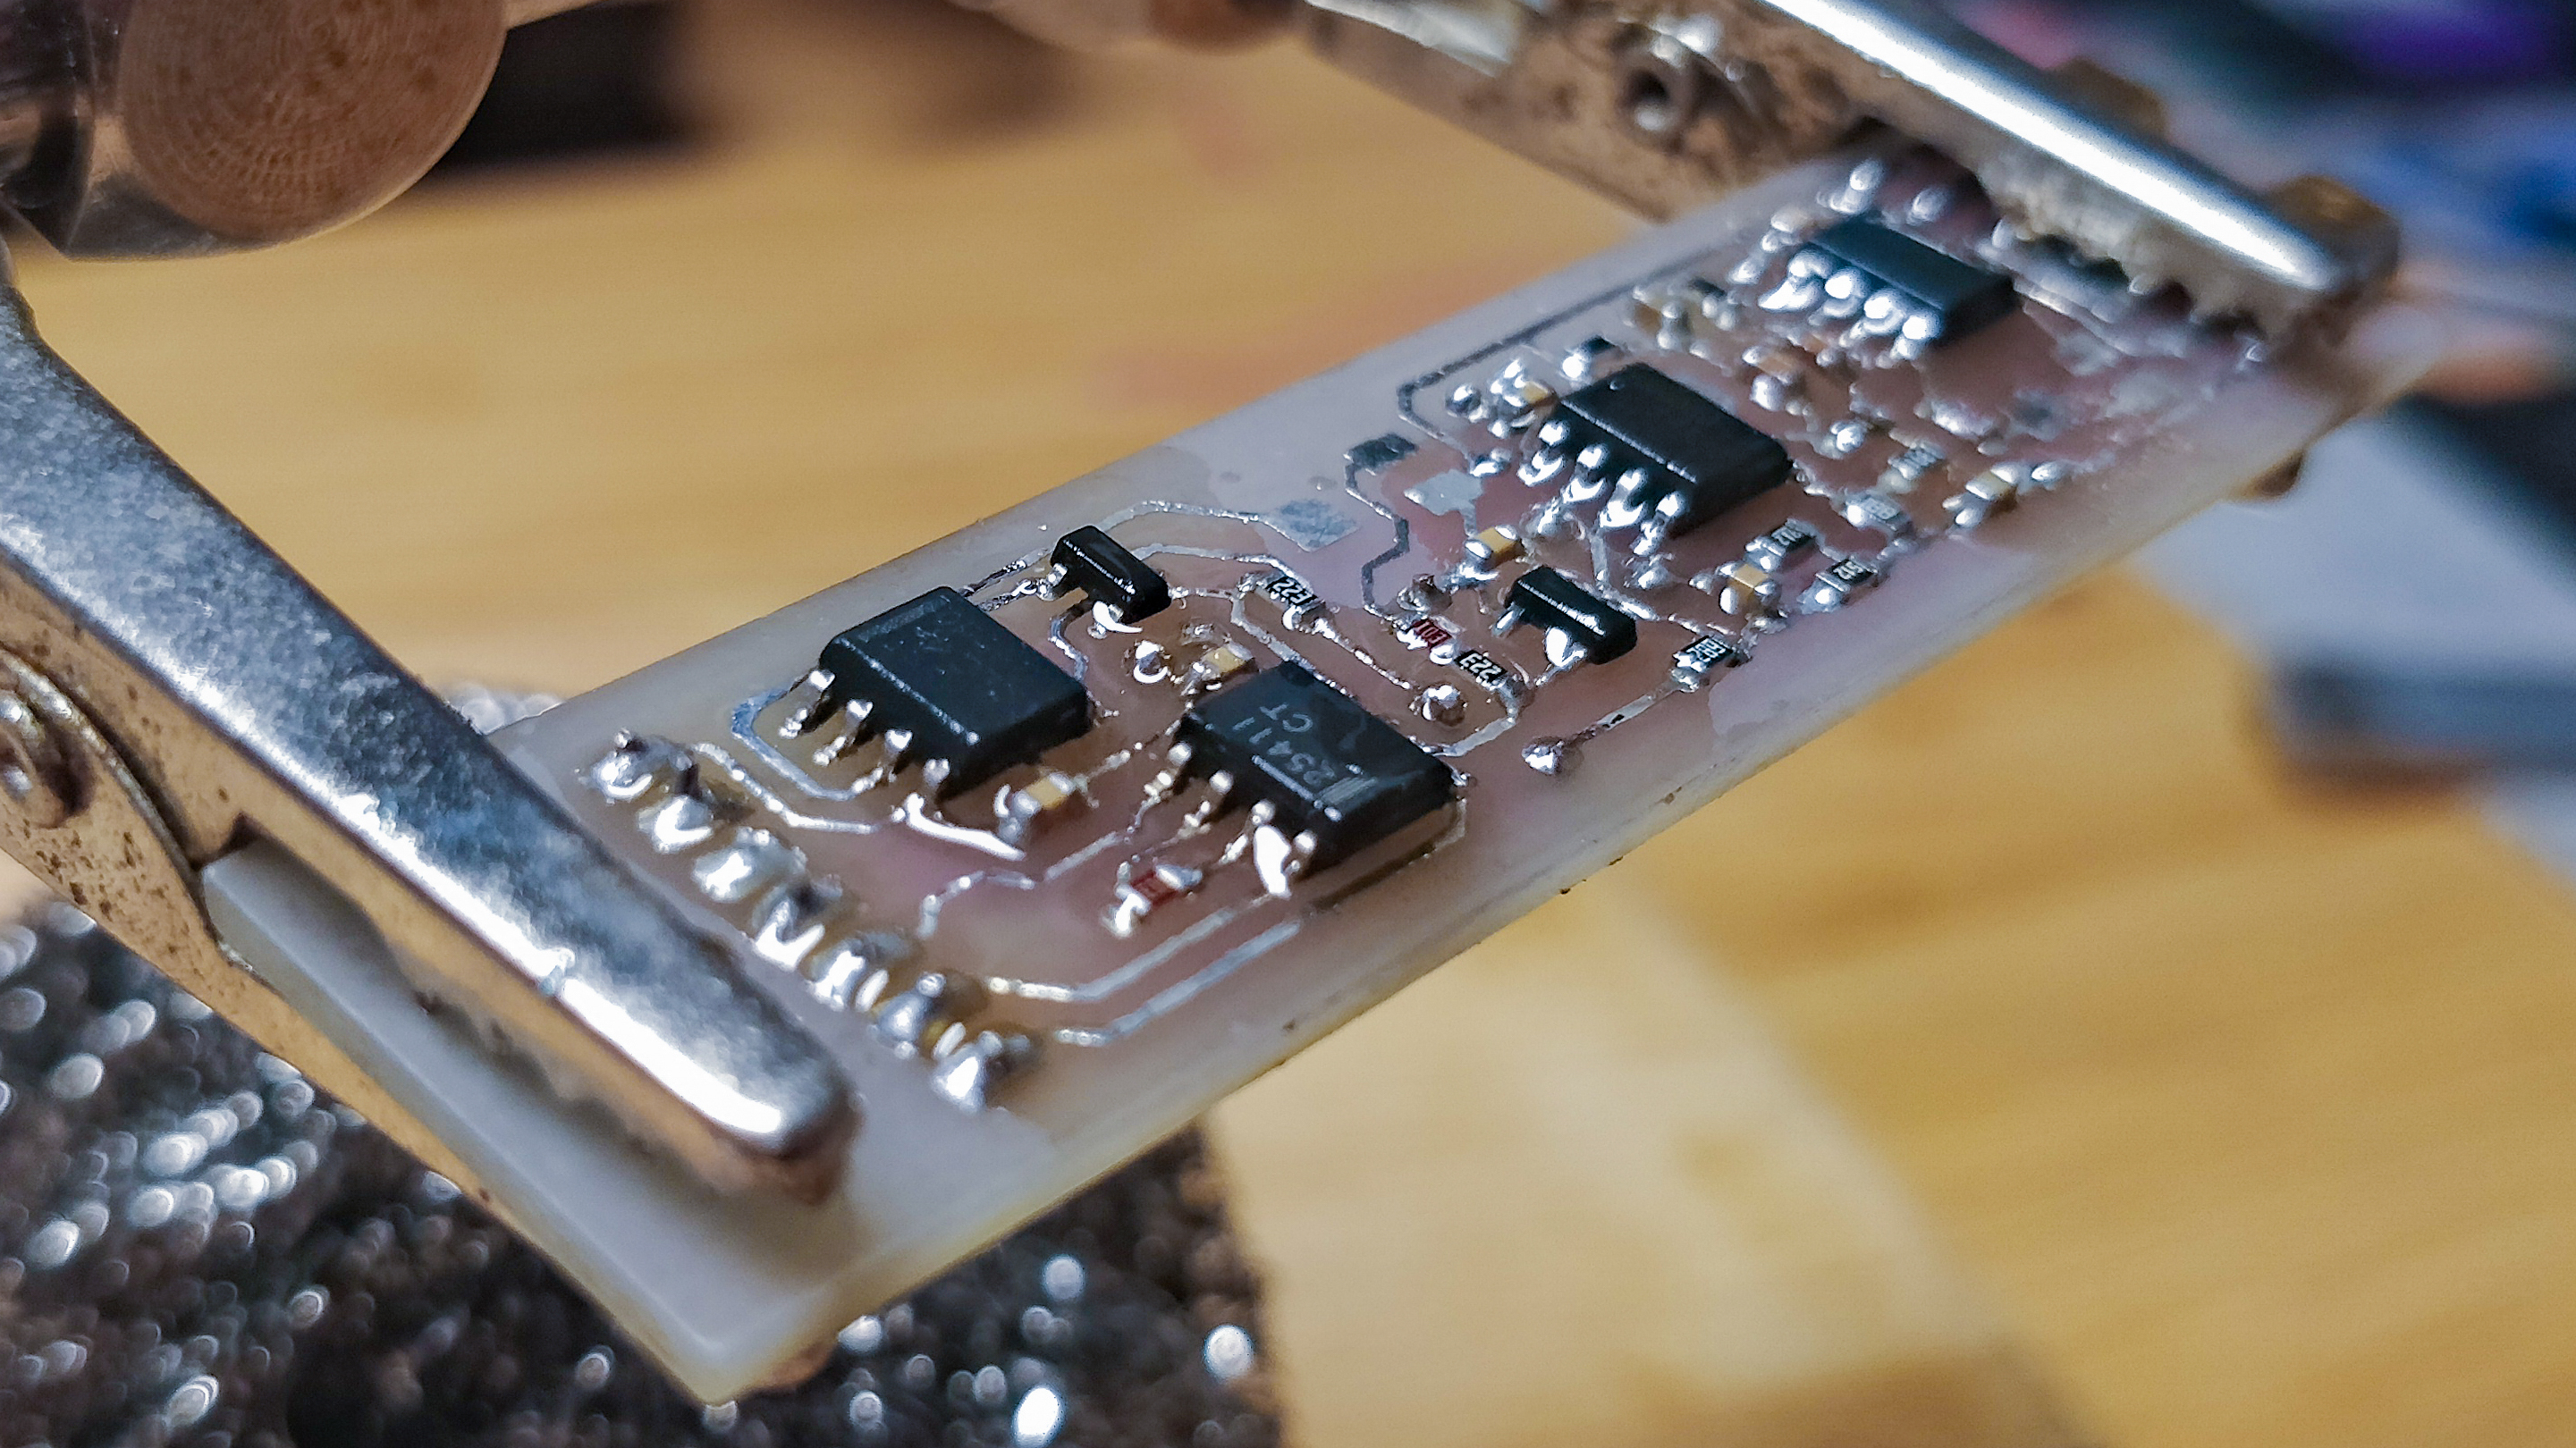
\includegraphics[width=\linewidth]{media/album/PSX_20220301_044735.jpg}
            \caption{}
            \label{fig:PhotoPCBProgress3}
        \end{minipage}
        \\
        \vspace*{.01\linewidth}
        \begin{minipage}[H]{.95\linewidth}
            \centering
            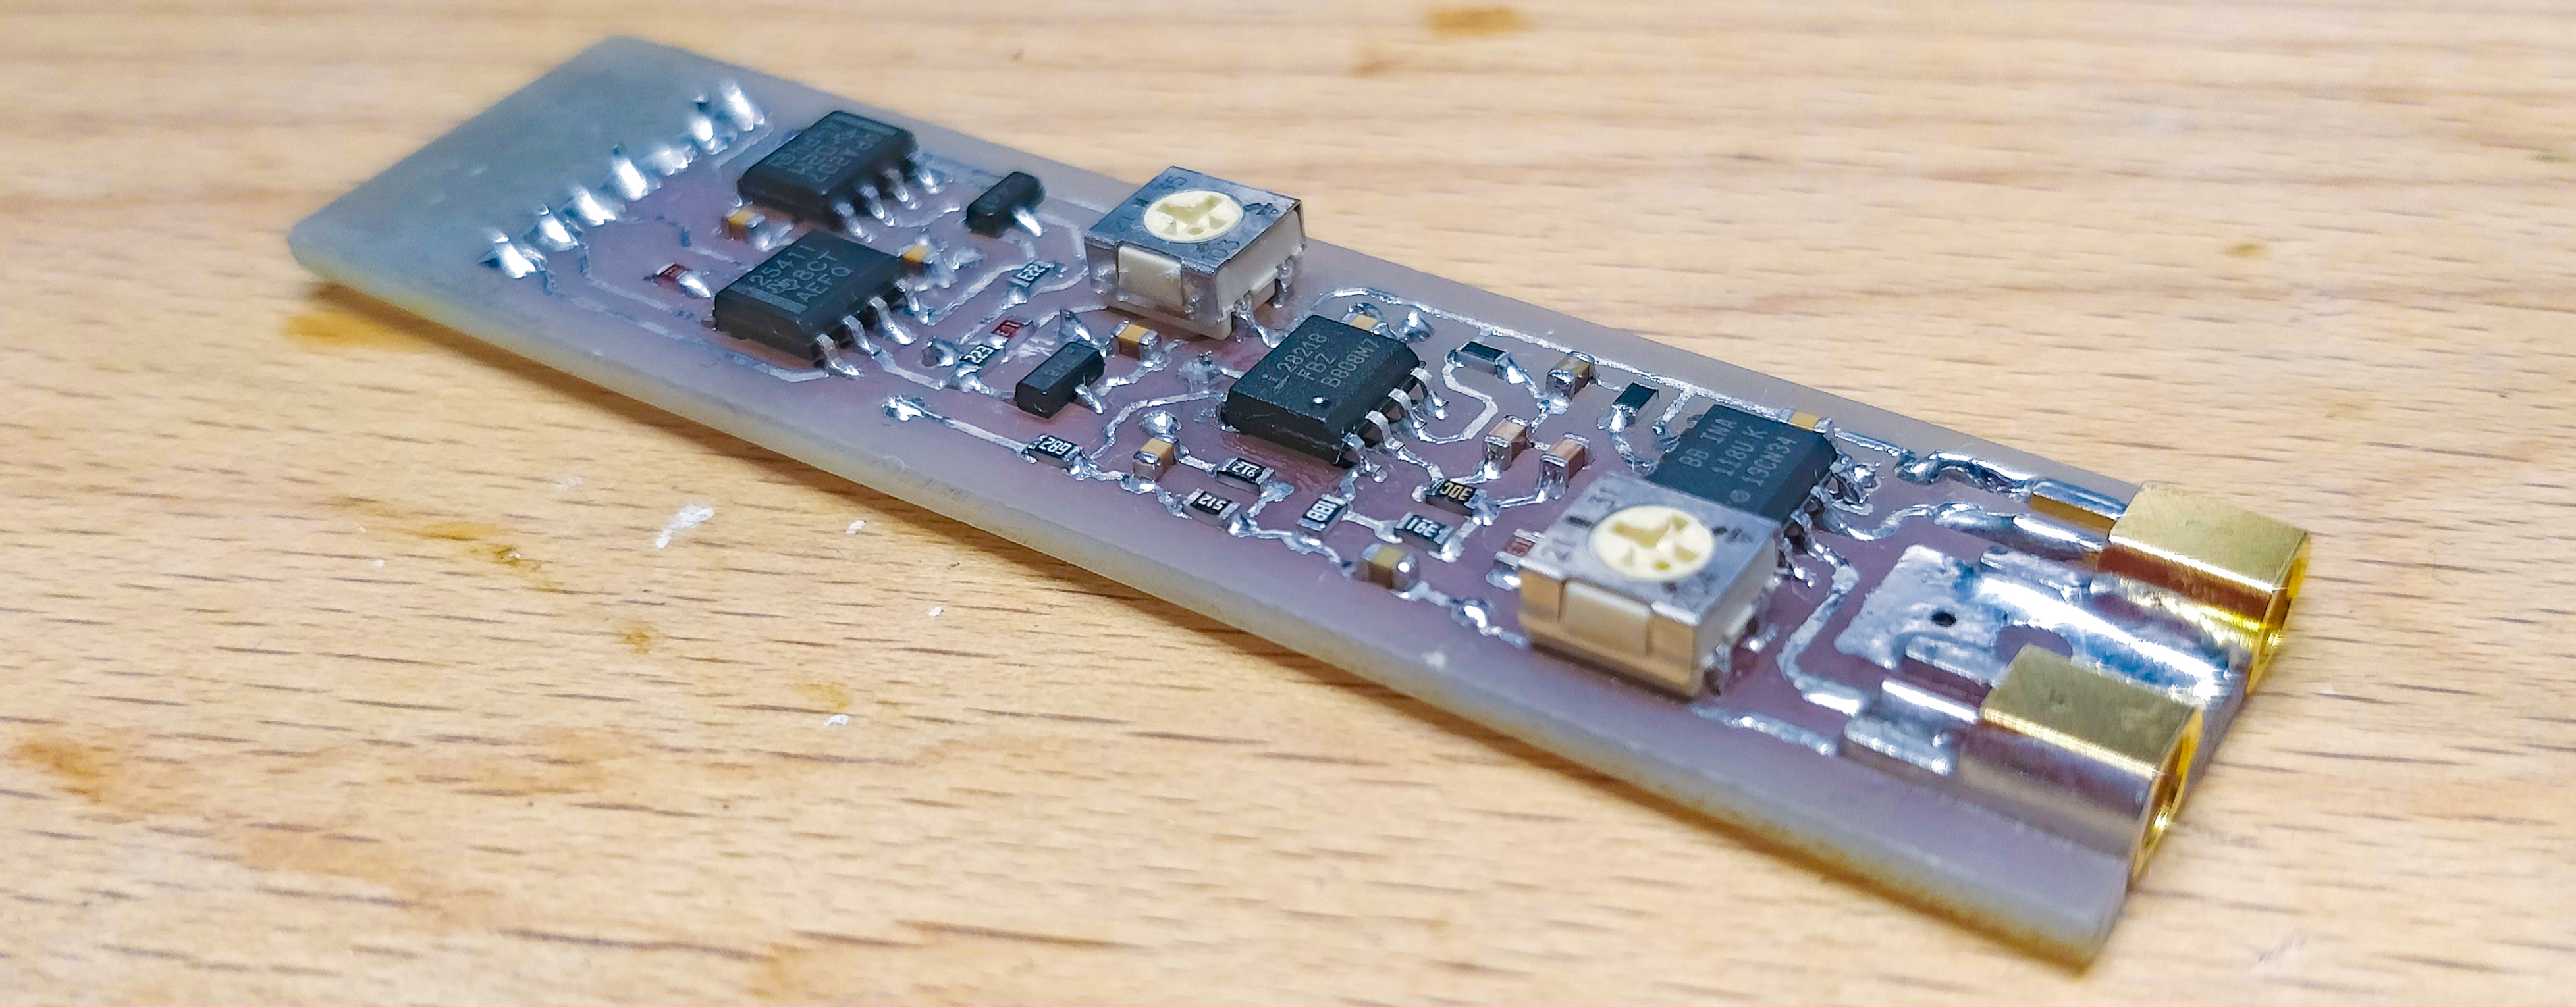
\includegraphics[width=\linewidth]{media/album/PSX_20220228_020356.jpg}
            \caption{}
            \label{fig:PhotoPCBDone}
        \end{minipage}
    \end{figure}

    Per un piccolo errore di ordine non ho avuto la possibilit\`{a} di saldare il connettore $J3$, per questo al suo posto ho saldato dei cavi. Con la saldatura dei cavi\footnote{Figure \ref{fig:PhotoCableProgress1}, \ref{fig:PhotoCableProgress2}, \ref{fig:PhotoCableProgress3}, \ref{fig:PhotoCableProgress4}, \ref{fig:PhotoCableProgress5}, \ref{fig:PhotoCableDone}} dei elettrodi il circuito era completo.
    \begin{figure}[H]
        \RaggedRight
        \centering   
        \begin{minipage}[H]{.95\linewidth}
            \centering
            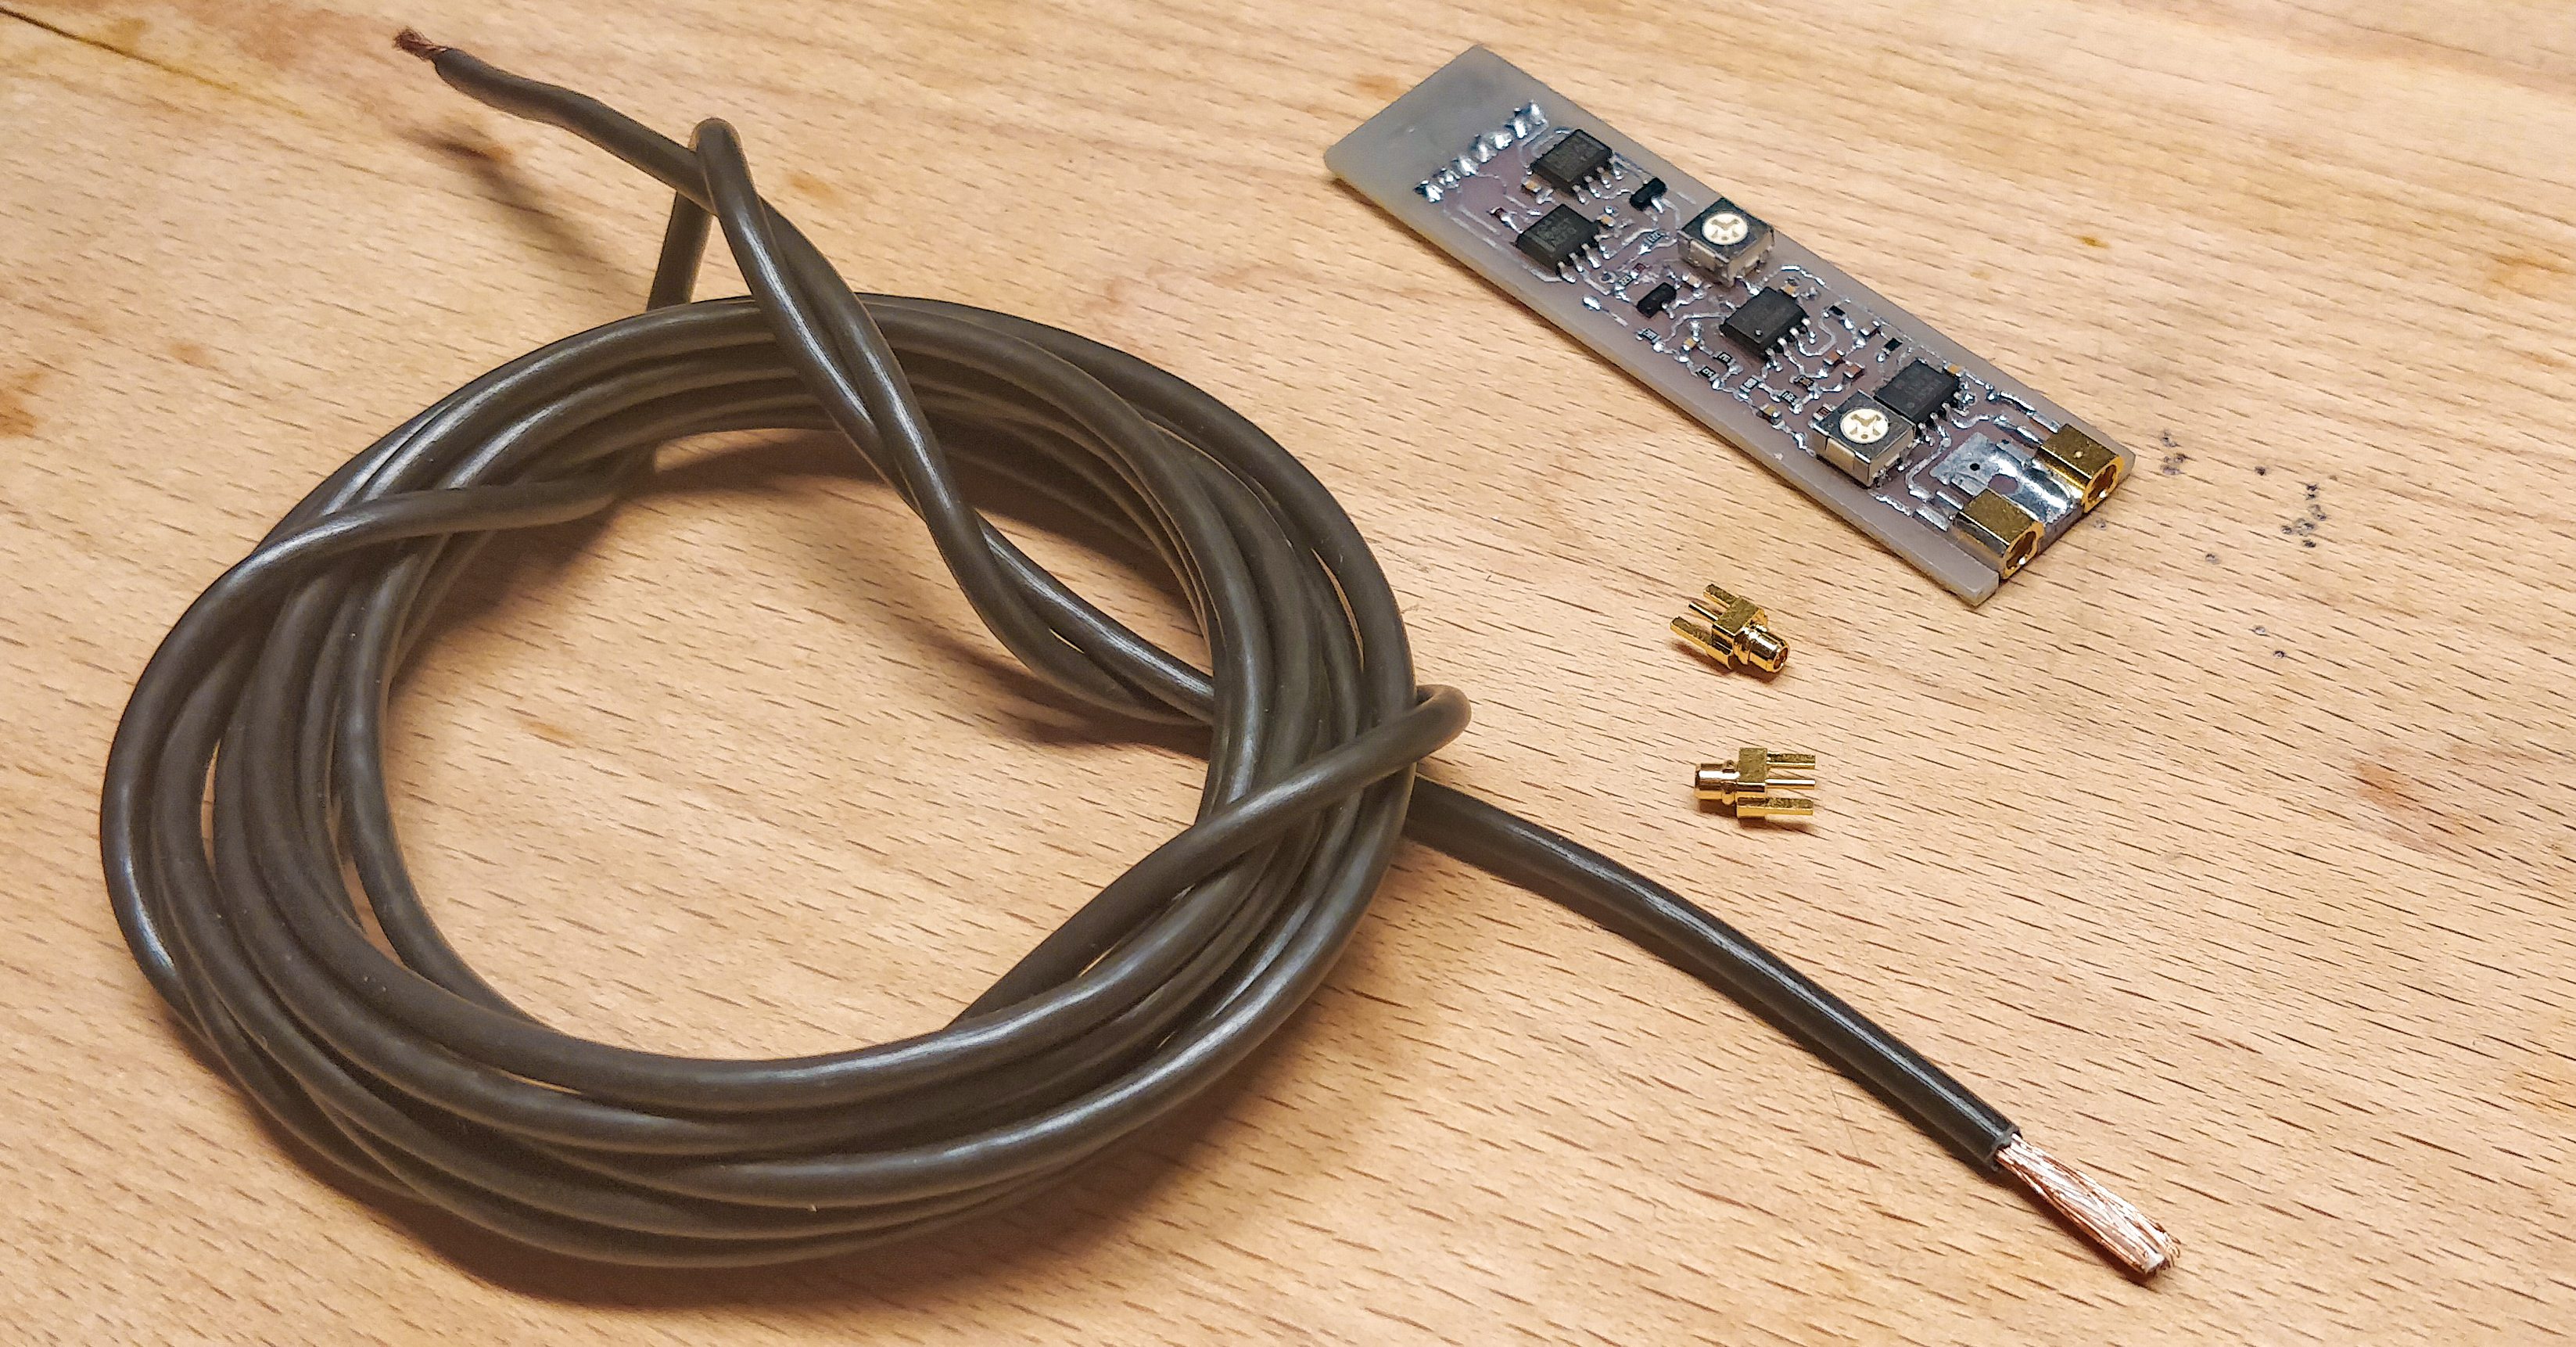
\includegraphics[width=\linewidth]{media/album/PSX_20220228_020856.jpg}
            \caption{}
            \label{fig:PhotoCableProgress1}
        \end{minipage}
        \\
        \vspace*{.01\linewidth}
        \begin{minipage}[H]{.28\linewidth}
            \centering
            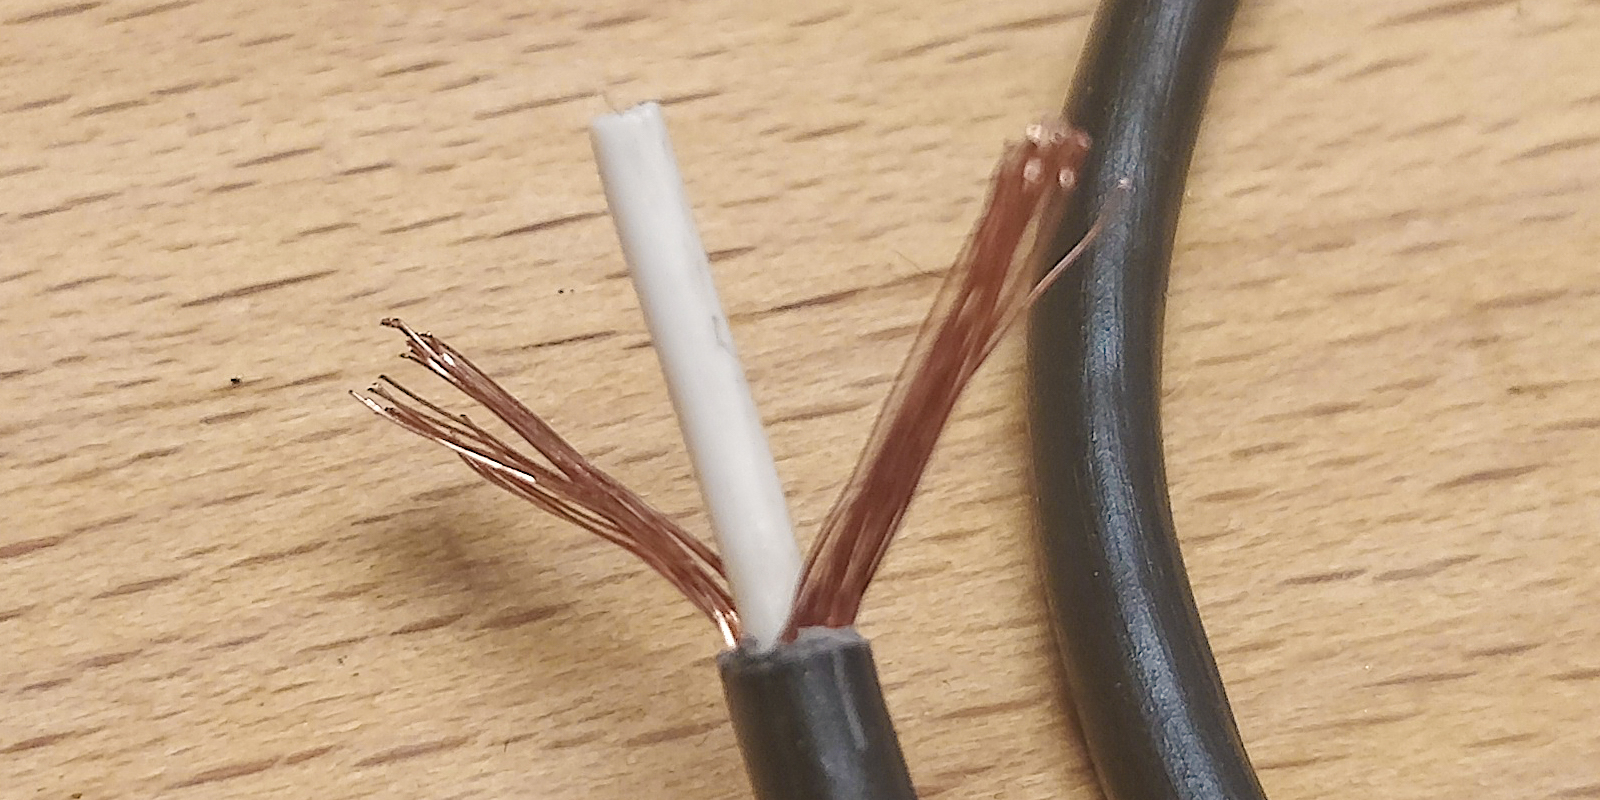
\includegraphics[width=\linewidth]{media/album/PSX_20220228_020741.jpg}
            \caption{}
            \label{fig:PhotoCableProgress2}
        \end{minipage}
        \hspace{.04\linewidth}
        \begin{minipage}[H]{.28\linewidth}
            \centering
            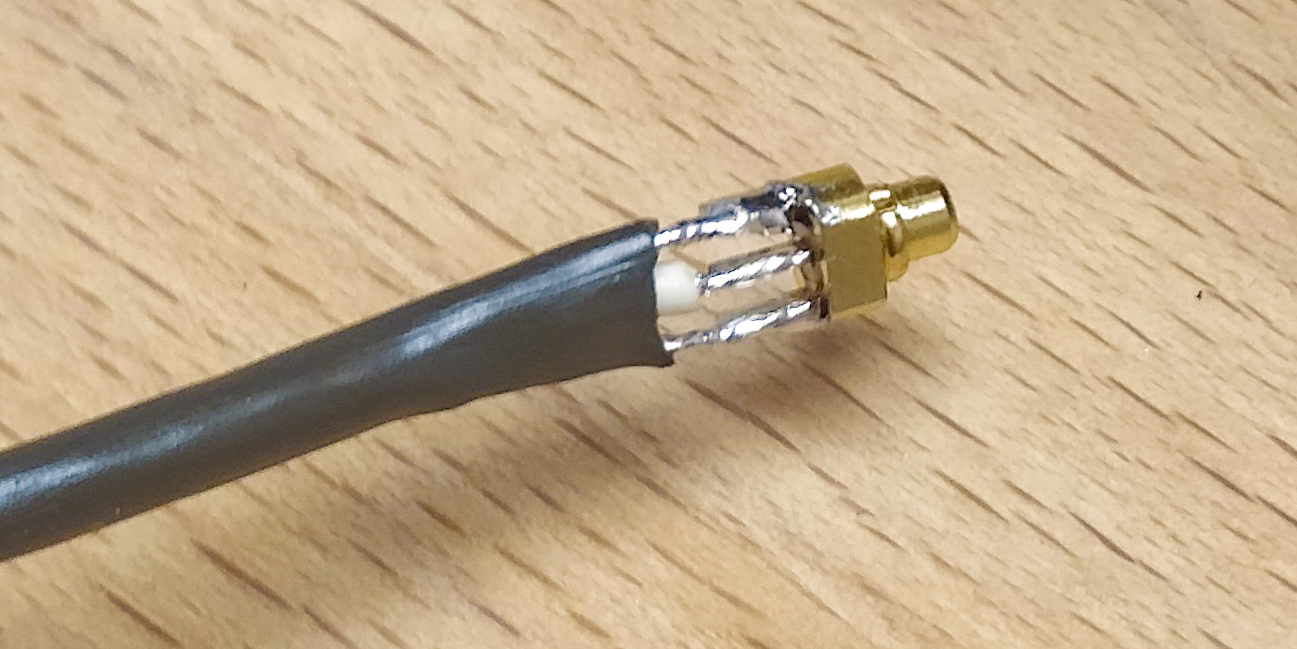
\includegraphics[width=\linewidth]{media/album/PSX_20220228_162153.jpg}
            \caption{}
            \label{fig:PhotoCableProgress3}
        \end{minipage}
        \hspace{.04\linewidth}
        \begin{minipage}[H]{.28\linewidth}
            \centering
            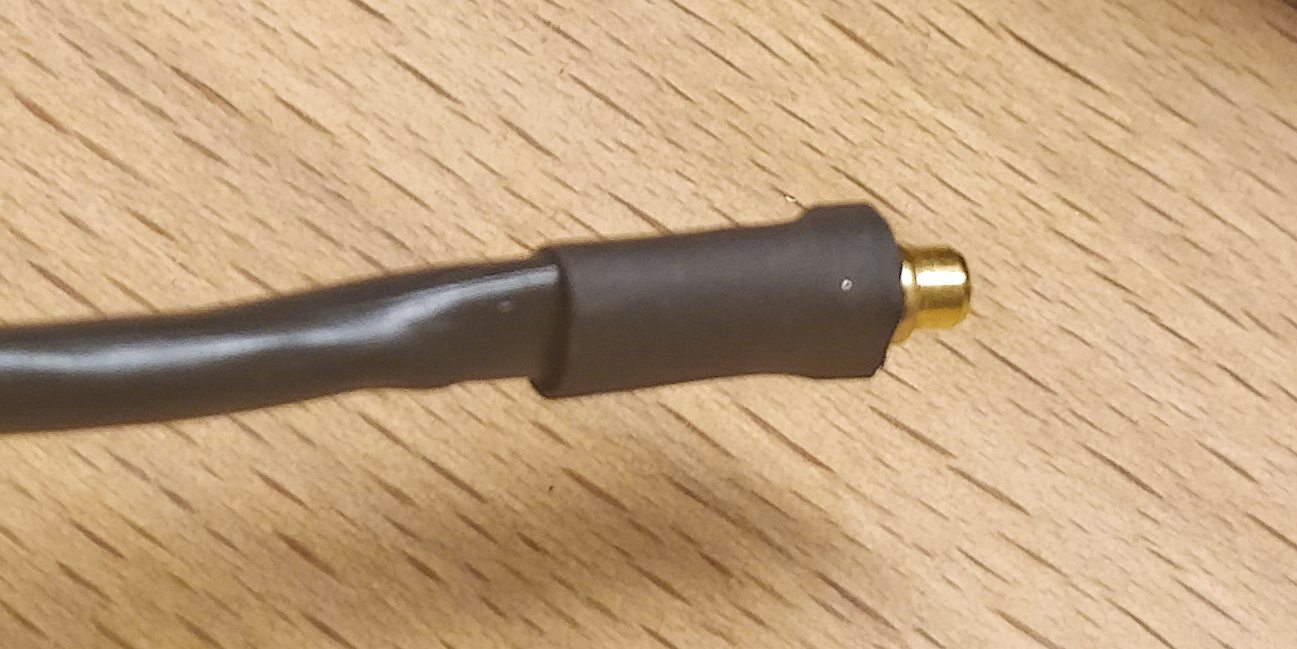
\includegraphics[width=\linewidth]{media/album/PSX_20220228_162233.jpg}
            \caption{}
            \label{fig:PhotoCableProgress4}
        \end{minipage}
        \\
        \vspace*{.01\linewidth}
        \begin{minipage}[H]{.95\linewidth}
            \centering
            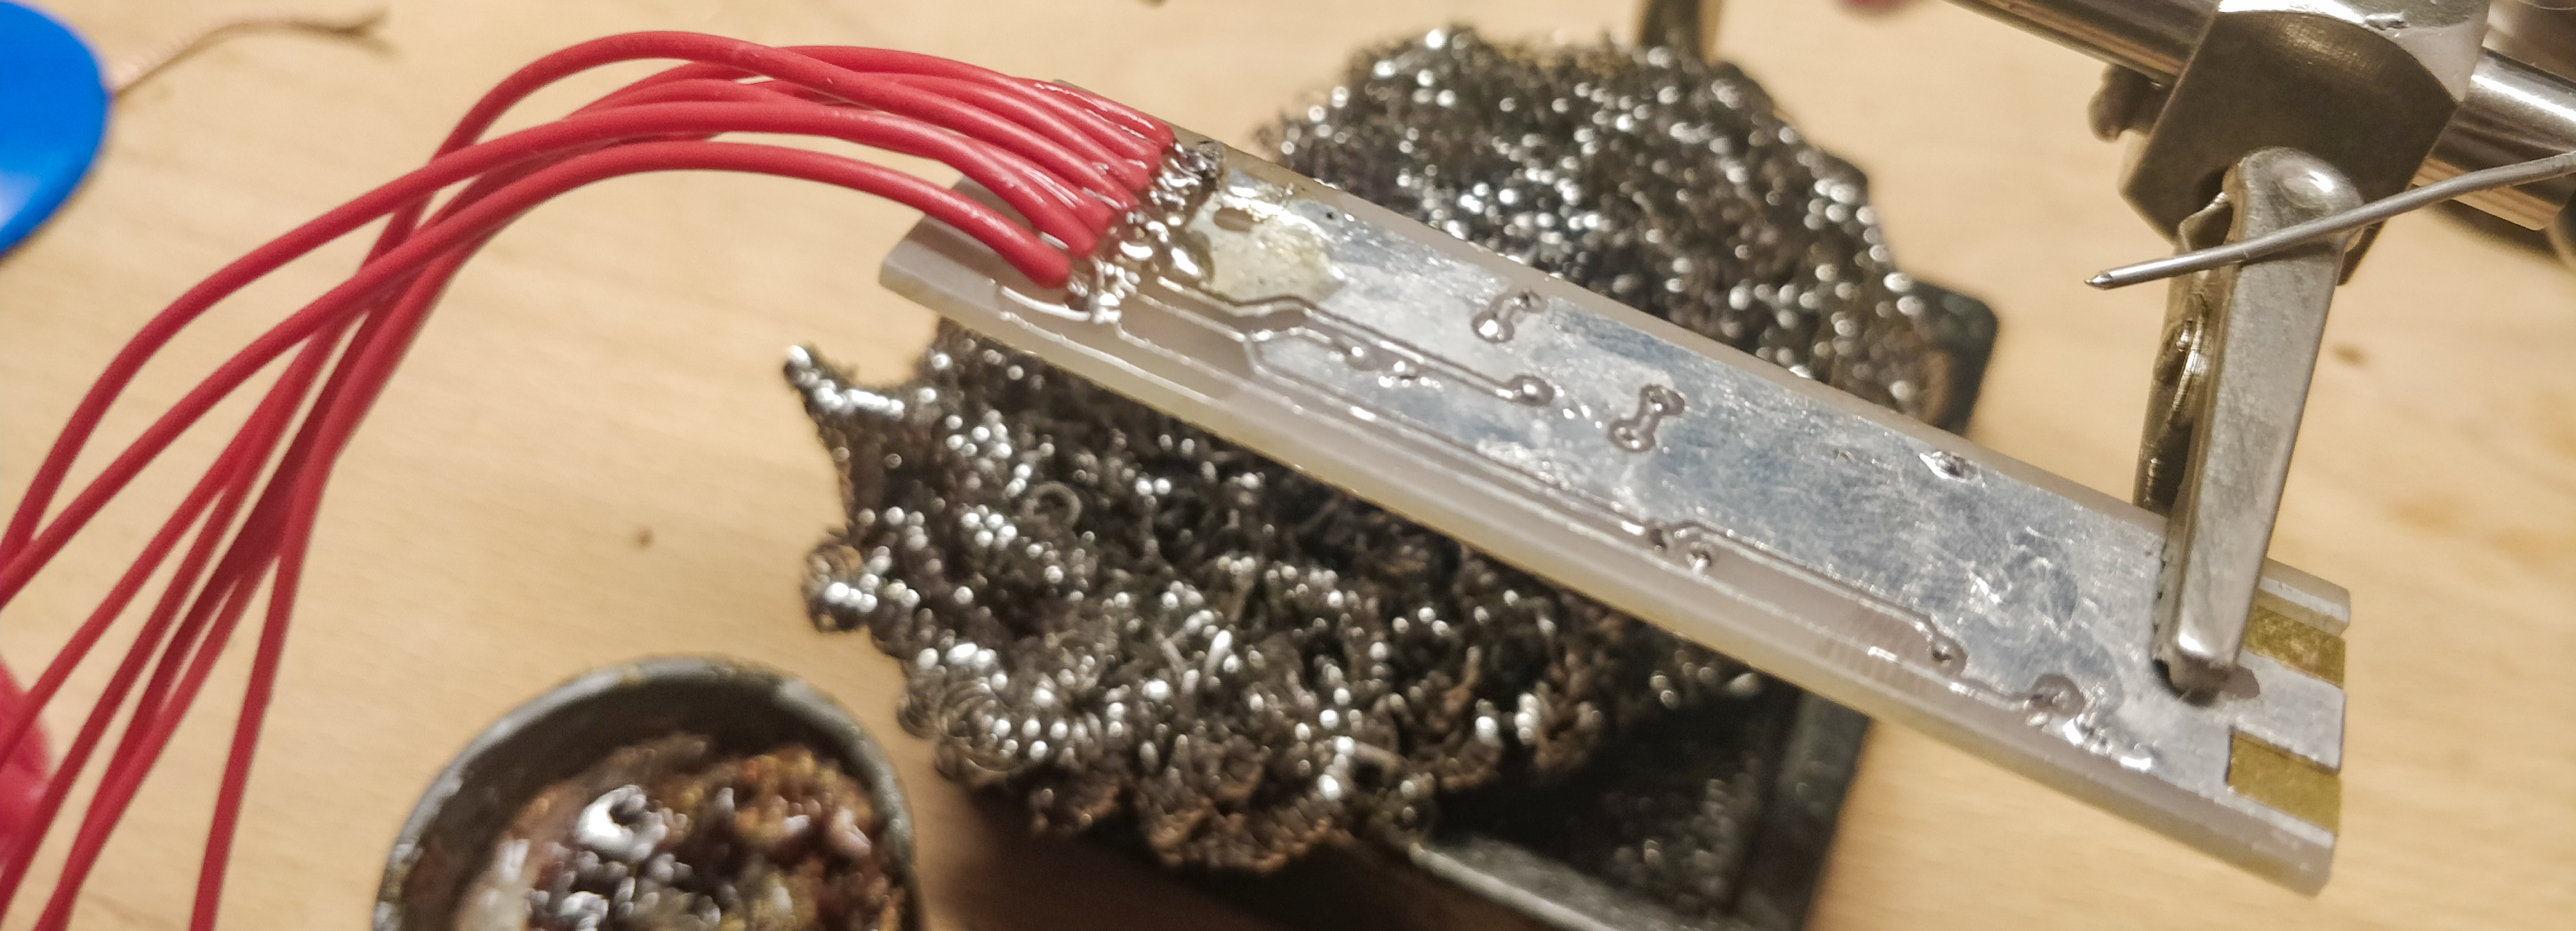
\includegraphics[width=\linewidth]{media/album/PSX_20220228_020557.jpg}
            
            \caption{}
            \label{fig:PhotoCableProgress5}
        \end{minipage}
        \\
        \vspace*{.01\linewidth}
        \begin{minipage}[H]{.95\linewidth}
            \centering
            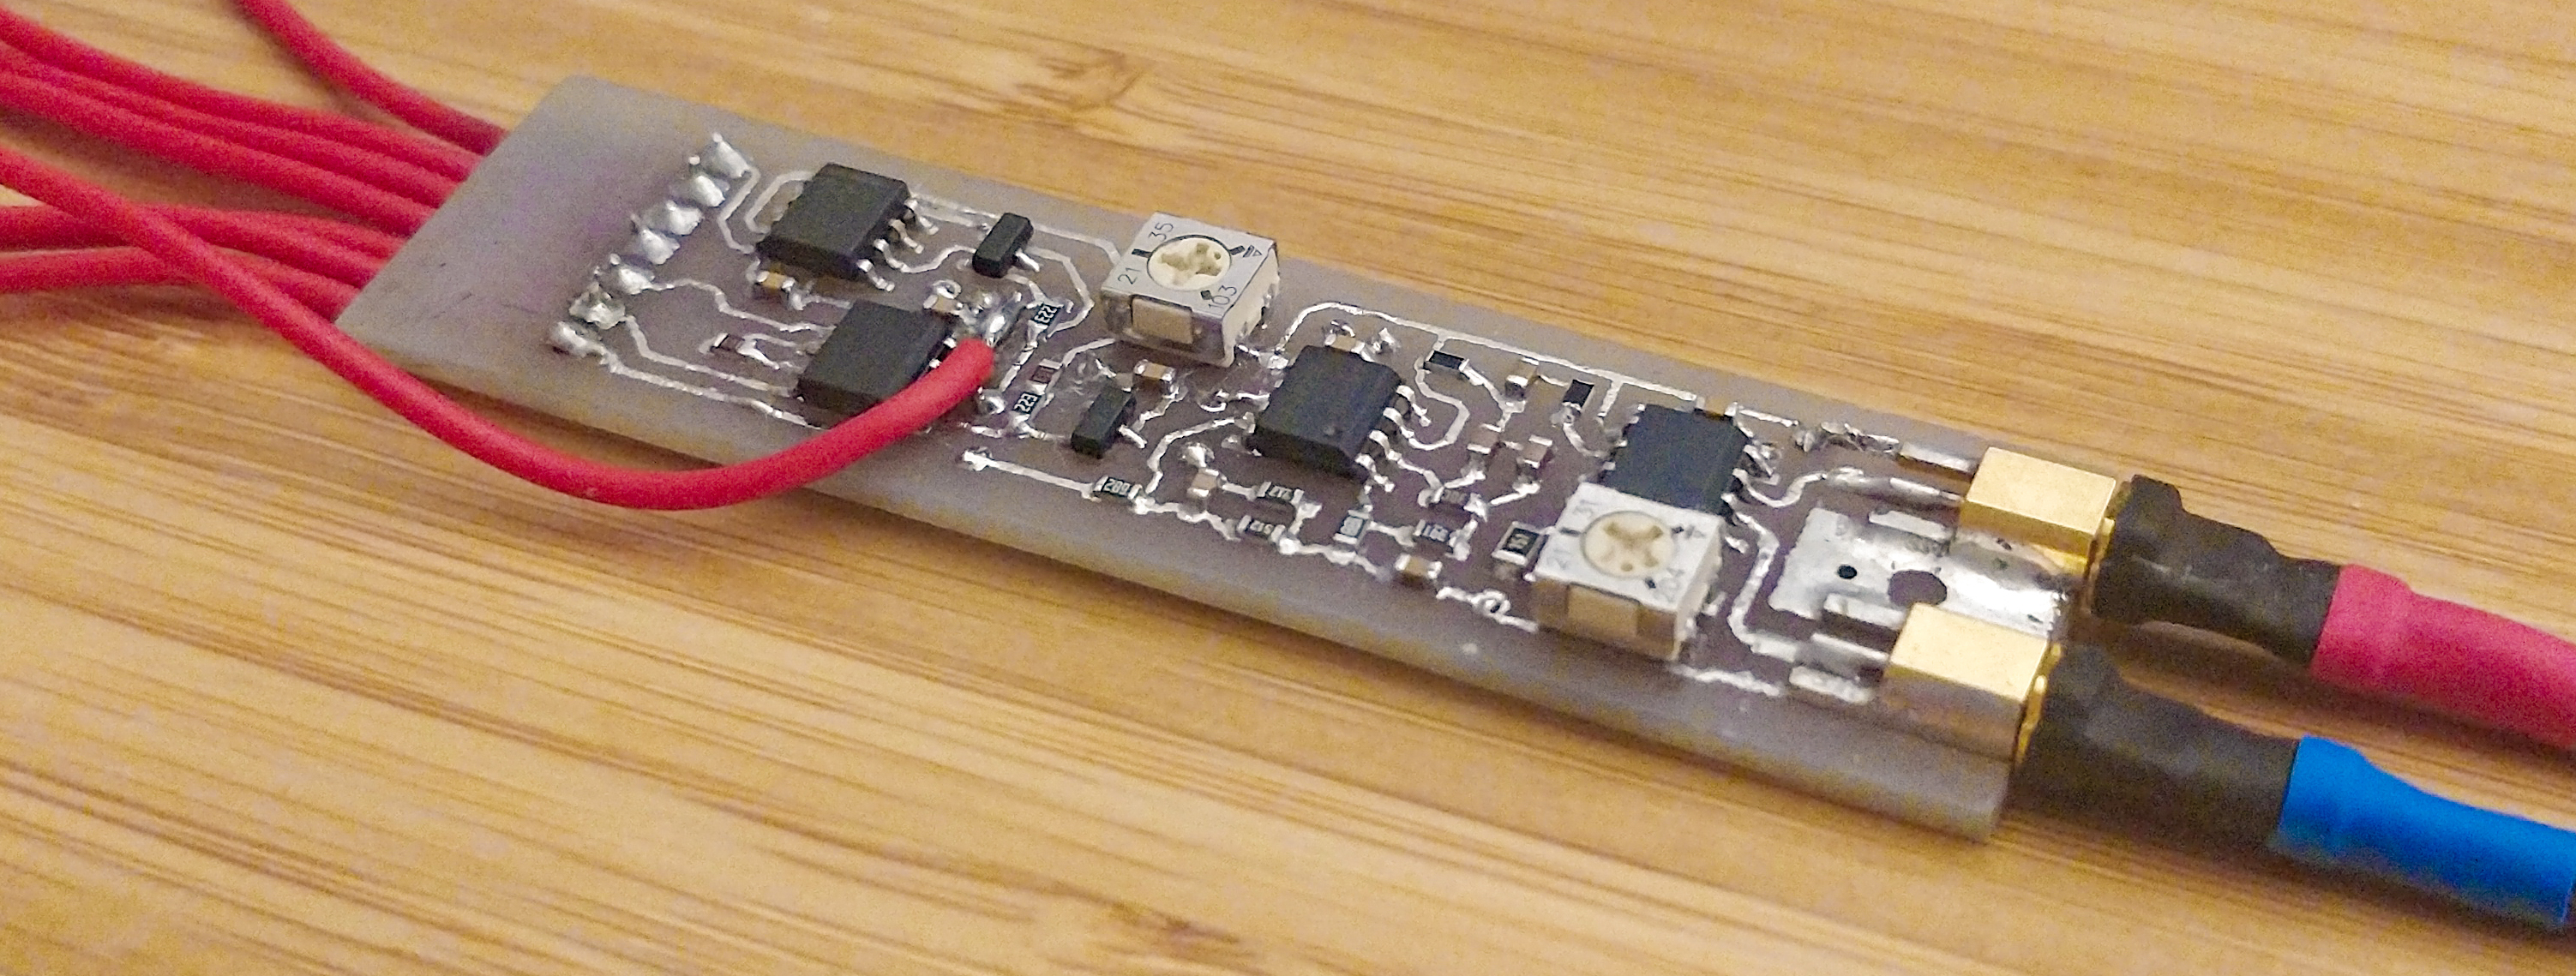
\includegraphics[width=\linewidth]{media/album/PSX_20220227_234925.jpg}
            \caption{}
            \label{fig:PhotoCableDone}
        \end{minipage}
    \end{figure}


    \subsection{Connessione}
    Ho connesso il circuito nel modo come era previsto dal circuito:
    \begin{center}
    \begin{tabular}{ ||l|l|| }
        \hline
        \multicolumn{1}{||l|}{Scheda Sensore} & \multicolumn{1}{|l||}{Arduino Due \& Regolatore} \\
        \hline
        \hline
        CS\footnote{Chip Select, o selezione del chip} & pin 4\footnote{Va bene un pin digitale qualsiasi}\\ 
        \hline
        SDO\footnote{Serial Data Output, o uscita delle informazioni seriali} & MISO\\  
        \hline
        SCLK\footnote{Serial Clock, o pin seriale che si occupa a dare il ritmo della trasmissione dei dati} & SCLK\\
        \hline
        $5V$   & $5V$\\
        \hline
        $3V3$  & $3.3V$\\
        \hline
        $-3V3$ & $-3.3V$ (Regolatore)\\
        \hline
        GND    & GND\\
        \hline
    \end{tabular}
    \end{center}
    \noindent Per scoprire che l'ADC non funziona per un motivo a me ignoto\footnote{L'SDO dell'ADC rimaneva sempre "$0$": $0-20mV$}.
    Allora ho deciso di utilizzare la porta analogica dell'Arduino DUE con un ADC di 10bit.

    \noindent La nuova connessione \`{e} la seguente
    \begin{center}
        \begin{tabular}{ ||l|l|| }
            \hline
            \multicolumn{1}{||l|}{Scheda Sensore} & \multicolumn{1}{|l||}{Arduino Due \& Regolatore} \\
            \hline
            \hline
            Uscita del nodo di rettificazione\footnote{SEMG Sensor Board - RECT} & A0\footnote{La porta analogica dell'Arduino DUE}\\
            \hline
            $5V$   & $5V$\\
            \hline
            $3V3$  & $3.3V$\\
            \hline
            $-3V3$ & $-3.3V$ (Regolatore)\\
            \hline
            GND    & GND\\
            \hline
        \end{tabular}
    \end{center}

    \begin{figure}[H]
        \centering
        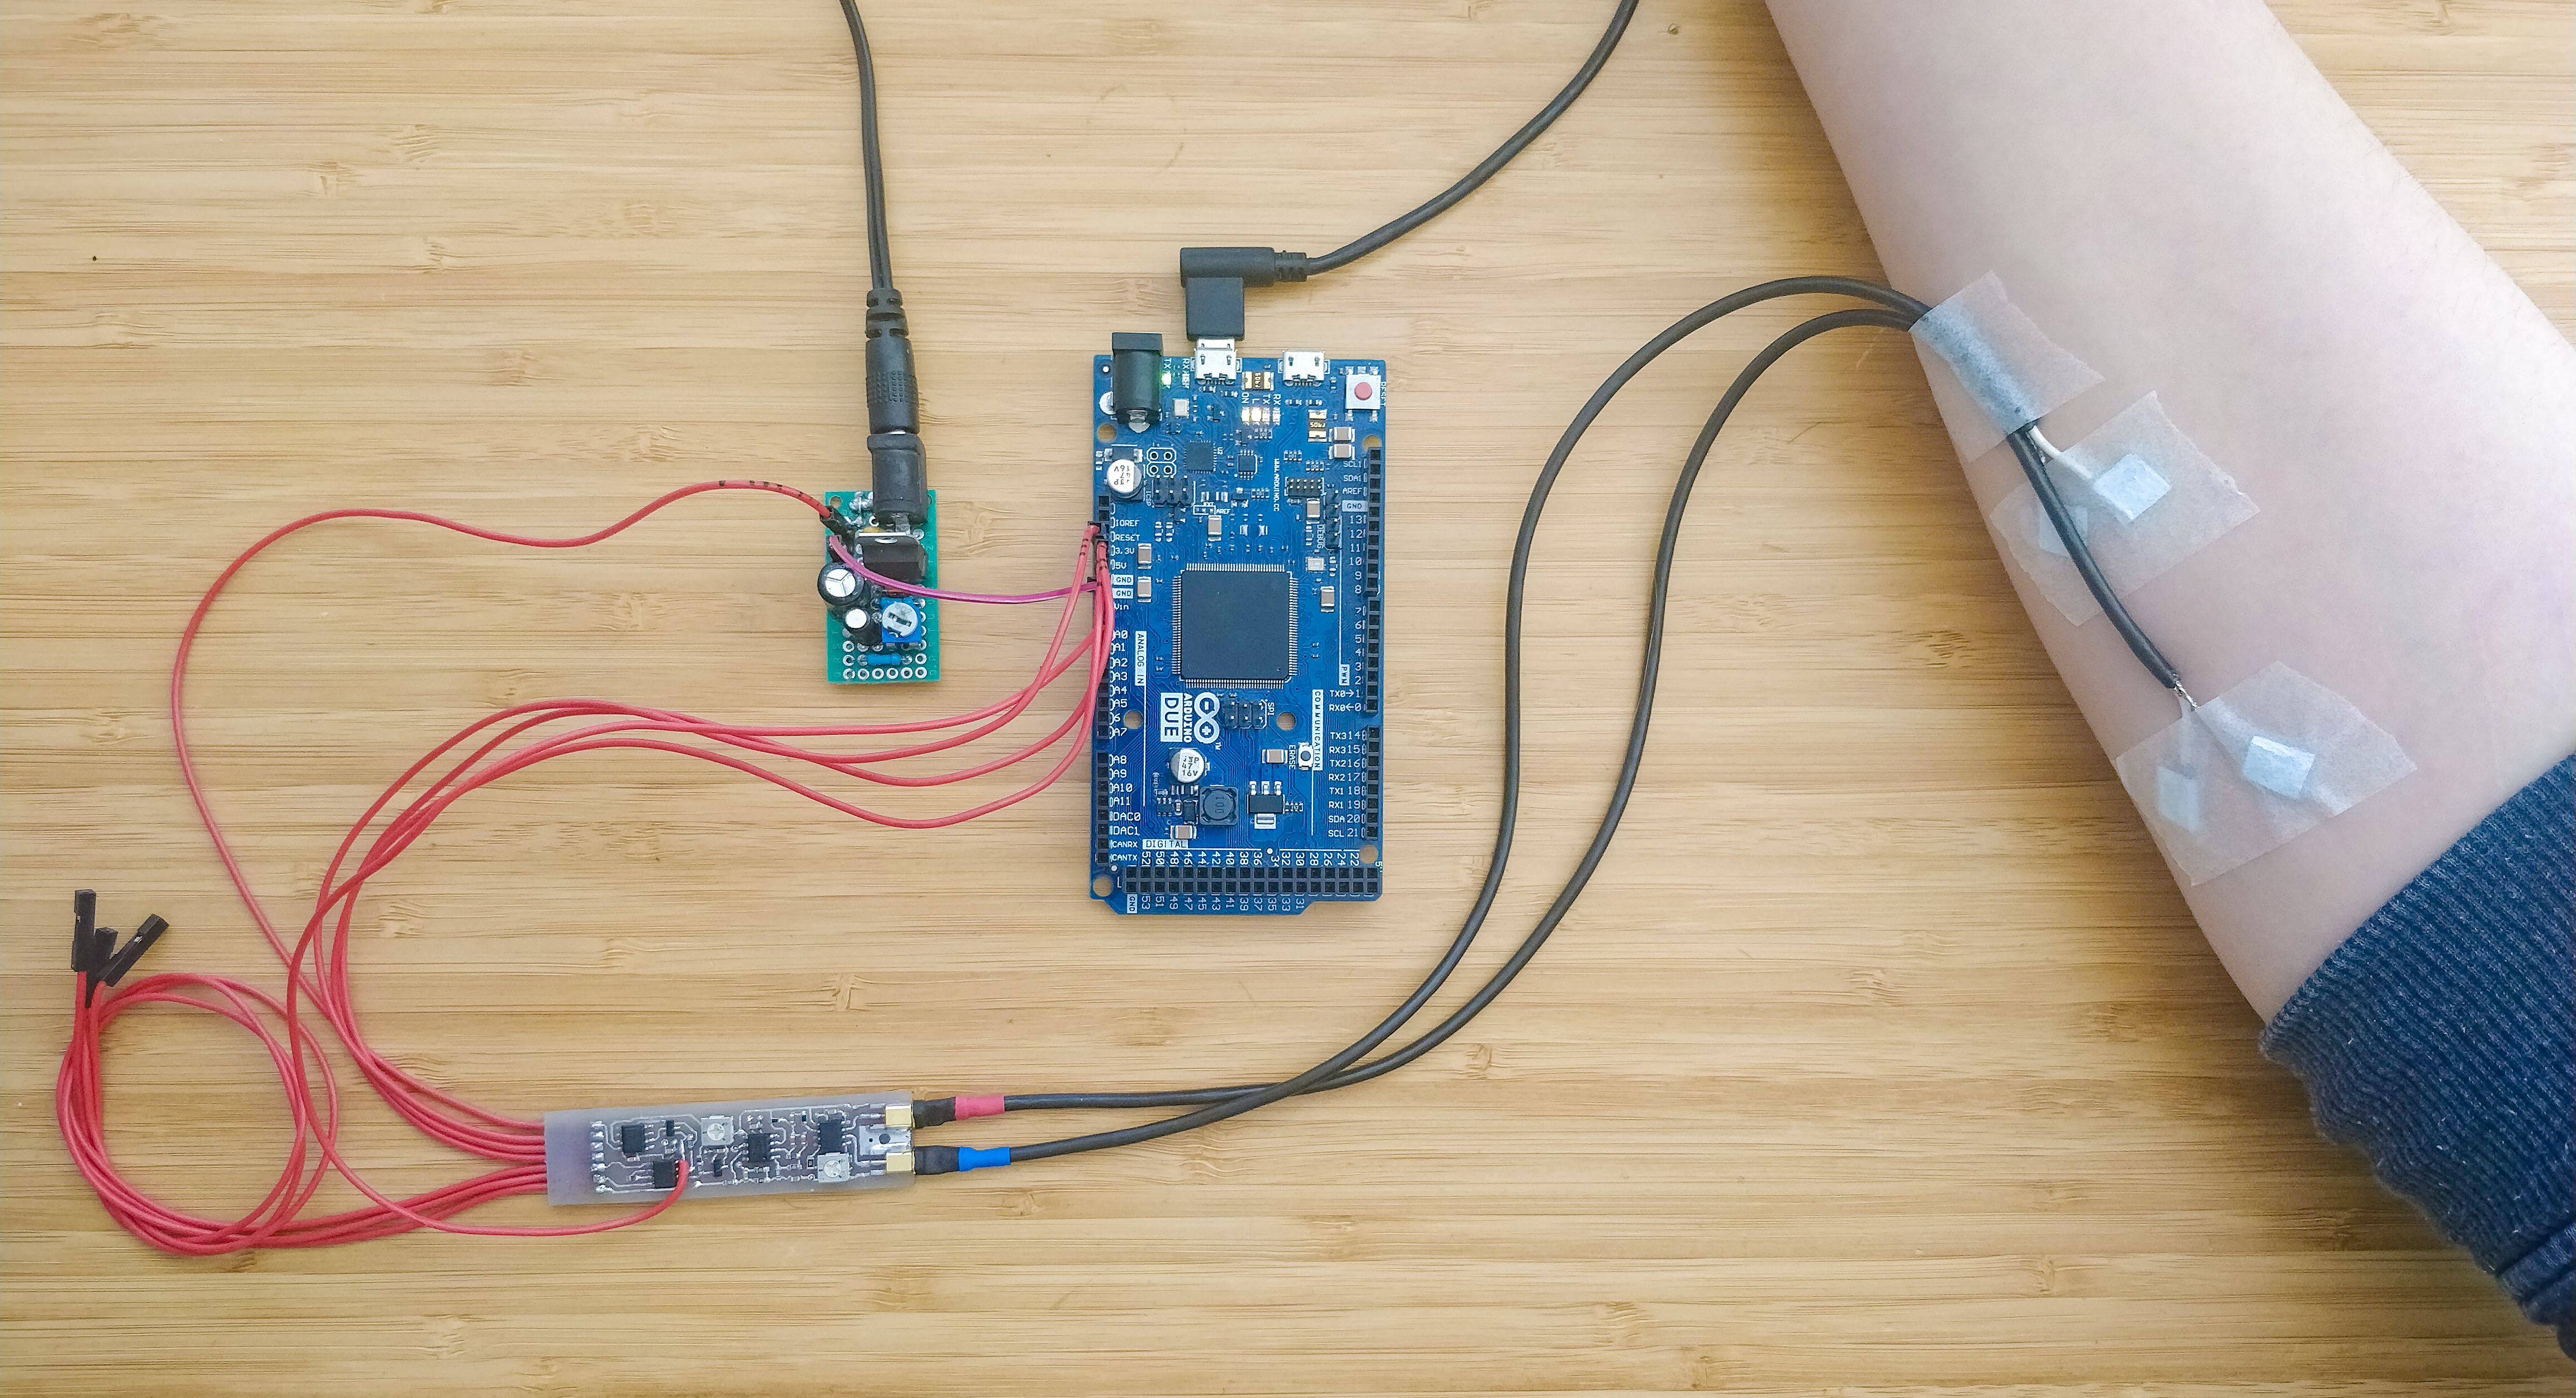
\includegraphics[width=\linewidth]{media/album/PSX_20220227_234659.jpg}
        \caption{Connessione di tutto il prototipo}
        \label{fig:AllConnection}
    \end{figure}
    
    \subsection{Software}
    Il codice per comunicare con l'ADC attraverso il protocollo SPI:
    \begin{verbatim}
        #include <Arduino.h>            // Importa la libreria di Arudino
        #include <SPI.h>                // Importa la libreria del protocollo SPI

        /* --------------------- */
        #define SS_PIN_TLV2541  4       // Pin digitale connesso al Chip Select dell'ADC
        #define FREQ_SAMPLE 1500        // Frequenza di lettura
        /* --------------------- */

        #define DELAY_INTERSAMPLE 1000000. / FREQ_SAMPLE  // Lunghezza della pausa tra 
                                                          // le letture

        SPISettings SPI_settings_TLV2541(10000000, MSBFIRST, SPI_MODE1);  // Dichiara
                                                                // le impostazioni
                                                                // dell'ADC per l'SPI

        void setup() {
            pinMode(SS_PIN_TLV2541, OUTPUT);            // Metti il Chip Select 
                                                        // dell'ADC nella
                                                        // modalita di uscita
            Serial.begin(115200);                       // Inizializza la porta SPI
            SPI.begin();                                // Inizializza la 
                                                        // comunicazione SPI
        }

        void loop() {
            digitalWrite(SS_PIN_TLV2541, LOW);          // Attiva l'ADC
            SPI.beginTransaction(SPI_settings_TLV2541); // Inizia trasmissione dati
                                                        // con impostazioni
                                                        // dell'ADC
            uint16_t val = SPI.transfer16(0x00);        // Leggi il valore in una
                                                        // variabile di 16 bit senza
                                                        // segno
            delayMicroseconds(4);                       // Dai del tempo all'ADC
                                                        // per convertire il segnale
            SPI.endTransaction();                       // Finisci trasmissione dati
            digitalWrite(SS_PIN_TLV2541, HIGH);         // Disabilita l'ADC

            Serial.println(val);                        // Stampa il valore nella porta
                                                        // seriale
            delayMicroseconds(DELAY_INTERSAMPLE);       // Aspetta il tempo predefinito
        }
    \end{verbatim}

    \noindent Il codice attuale per leggere il valore dalla porta analogica A0
    \begin{verbatim}
        #include <Arduino.h>          // Importa la libreria di Arudino

        /* --------------------- */
        #define SENSE_PIN A0          // Pin analogico
        #define FREQ_SAMPLE 1500      // Frequenza di lettura
        /* --------------------- */

        #define DELAY_INTERSAMPLE 1000000. / FREQ_SAMPLE  // Lunghezza della pausa tra
                                                          //le letture

        void setup() {
            Serial.begin(115200); // Inizia la comunicazione seriale
        }

        void loop() {
            Serial.println(analogRead(SENSE_PIN));  // Leggi il valore dal pin 
                                                    // analogico e invialo
                                                    // alla porta seriale
            delayMicroseconds(DELAY_INTERSAMPLE);   // Aspetta il tempo predefinito
        }
    \end{verbatim}

    Per visualizzare il grafico ho utilizzato il seguente programma gi\`{a} scritto in Processing \parenciteit{}{ProcessingGrapher:Software}
    \section{Risultati} \label{sec:Results}
    \begin{figure}[H]
        \centering
        \begin{minipage}[H]{\linewidth}
            \begin{tikzpicture}
                \begin{axis}[
                    axis x line=bottom,
                    axis y line*=left,
                    ylabel style={rotate=-90},
                    xlabel={$t[ms]$},
                    ylabel={$U[V]\cdot k$},
                    legend entries={$($Canale $1)$},
                    legend pos=north east,
                    height=.4\textwidth,
                    width=.85\textwidth,
                    smooth,
                    clip=true,
                    xmin=0,
                    % xmax=17500,
                    colormap/twilight_shifted,
                    axis_style_default_data,
                    ymajorgrids=true,
                    xmajorgrids=false,
                    grid style=dashed,
                    cycle list={[colors of colormap={145,250},]},
                    every axis plot/.append style={mark=none, thick, draw opacity=.7},
                    ]
                    % [2026 revision] measured signal in solid dark teal (was twilight_shifted
                    % mid-range + draw opacity .7; user request: clearer "real measured" color)
                    \addplot[draw=teal!70!black, draw opacity=1] table [header=false, col sep=comma]{datasets/result/gr1.csv};
                \end{axis}
            \end{tikzpicture}
            \subcaption{Dimostrazione della possibilit\`{a} di lettura del segnale}
        \end{minipage}
        \begin{minipage}[H]{\linewidth}
            \begin{tikzpicture}
                \begin{axis}[
                    axis x line=bottom,
                    axis y line*=left,
                    ylabel style={rotate=-90},
                    xlabel={$t[ms]$},
                    ylabel={$U[V]\cdot k$},
                    legend entries={$($Canale $1)$},
                    legend pos=north east,
                    height=.4\textwidth,
                    width=.85\textwidth,
                    smooth,
                    clip=true,
                    xmin=0,
                    % xmax=17500,
                    colormap/twilight_shifted,
                    axis_style_default_data,
                    ymajorgrids=true,
                    xmajorgrids=false,
                    grid style=dashed,
                    cycle list={[colors of colormap={145,250},]},
                    every axis plot/.append style={mark=none, thick, draw opacity=.7},
                    ]
                    \addplot[draw=teal!70!black, draw opacity=1] table [header=false, col sep=comma]{datasets/result/gr2.csv};
                \end{axis}
            \end{tikzpicture}
            \subcaption{Dimostrazione della possibilit\`{a} di aggiustare l'ampiezza del segnale \emph{(Le prime tre contrazioni dei muscoli sono su una soglia di amplificazione, mentre le prossime due sono su un'altra che \`{e} chiaramente minore)}}
        \end{minipage}
        \begin{minipage}[H]{\linewidth}
            \begin{tikzpicture}
                \begin{axis}[
                    axis x line=bottom,
                    axis y line*=left,
                    ylabel style={rotate=-90},
                    xlabel={$t[ms]$},
                    ylabel={$U[V]\cdot k$},
                    legend entries={$($Canale $1)$},
                    legend pos=north east,
                    height=.4\textwidth,
                    width=.85\textwidth,
                    smooth,
                    clip=true,
                    xmin=0,
                    % xmax=17500,
                    colormap/twilight_shifted,
                    axis_style_default_data,
                    ymajorgrids=true,
                    xmajorgrids=false,
                    grid style=dashed,
                    cycle list={[colors of colormap={145,250},]},
                    every axis plot/.append style={mark=none, thick, draw opacity=.7},
                    ]
                    \addplot[draw=teal!70!black, draw opacity=1] table [header=false, col sep=comma]{datasets/result/gr3.csv};
                \end{axis}
            \end{tikzpicture}
            \subcaption{Dimostrazione della possibilit\`{a} di aggiustare l'altezza del segnale}
        \end{minipage}
        \caption{Segnali campionati provvenienti dalla scheda sensore durante una serie di contrazioni della mano \emph{(Segnale pi\`{u} ampio vuole dire che il muscolo \`{e} in contrazione)}}
    \end{figure}
    Avendo mostrato questo, posso considerare che il bersaglio del lavoro di maturit\`{a} \`{e} stato raggiunto.

    \section{Conclusioni}
    Ritengo questo prototipo un successo per la verifica di funzionamento per e tante conoscenze che ho assunto durante la ricerca.
    Nonostante dei piccoli errori\footnote{Come l'ADC non funzionante} che mi hanno impedito di verificare altri fattori come i rumori introdotti dal circuito, e l'adatta amplificazione del segnale sono riuscito a filtrare il segnale in modo adatto per poi ricevere un segnale abbastanza puro.
    Le numerose difficolt\`{a} che ho incontrato durante il design del progetto, che partivano dai problemi con il sistema operativo del computer e finivano con la perdita di tempo in internet per la ricerca di informazioni molto sparpagliate, mi hanno reso pi\`{u} sicuro delle mie capacit\`{a} e dei miei metodi per risolvere problemi.
    Il lavoro che si deve fare ancora fare per ottenere uno skate funzionante \`{e} non \`{e} molto pi\`{u} vasto del lavoro che ho fatto durante questo lavoro di maturit\`{a} perche\'{e} ritengo che il design dei circuiti analogici di elaborazione del segnale \`{e} una delle cose in assoluto pi\`{u} complesse dell'elettrotecnica.
    Inoltre sono anche contento che il mio progetto \`{e} stato fatto con tenendo conto delle previsioni nel futuro, anche se questa parte mi ha sottratto tanto tempo: per esempio la regolazione dell'amplificazione pu\`{o} essere facilmente sostituita da un potenziometro digitale\footnote{Un elemento che varia la propria resistenza usando dei protocolli di comunicazione digiali} per ottenere una funzionalit\`{a} di autocalibrazione e la poca corrente che consuma il circuito\footnote{Nei calcoli \`{e} presente anche questa parte} mi permette di scegliere quanto sofisticato voglio fare il circuito per eccesso di capacit\`{a} nella batteria (oppure di diminuire ancora di pi\`{u} il circuito e non temere il suo surriscaldamento).
    Infine sono contento non solo del lavoro che ho fatto, ma anche del come \`{e} stato fatto: da me stesso, con le proprie mani e la propria mente.

    \section{Calcoli} \label{sec:Calculations}
    In questa Sezione presento differenti documenti che ho ottenuto mentre utilizzavo Maple per calcolare diversi risultati.
    \begin{center}
        \begin{tabular}{ ||l|l|| }
            \hline
            \multicolumn{1}{||l|}{Titolo} & \multicolumn{1}{|l||}{Argomento} \\
            \hline
            \hline
            LPF Theor Model & Modello teorico della funzione di trasferimento di un LPF \\
            HPF Theor Model & Modello teorico della funzione di trasferimento di un HPF \\
            Transfer Function Derivation & Derivazione delle funzioni di trasferimento \\
            Voltage Regulator & Informazioni a riguardo del regolatore di tensione \\
            Voltage Reference & Informazioni a riguardo del riferimento di tensione \\
            Offset Amplification Tuning & Tuning della distribuzione dell'amplificazione nei diversi nodi del circuito \\
            Noise & Calcolo dei rumori introdotti dal circuito \\
            INA & Informazioni a riguardo dell'INA \\
            OA & Informazioni a riguardo dell'OA \\
            ADC & Informazioni a riguardo dell'ADC \\
            \hline
        \end{tabular}
    \end{center}

    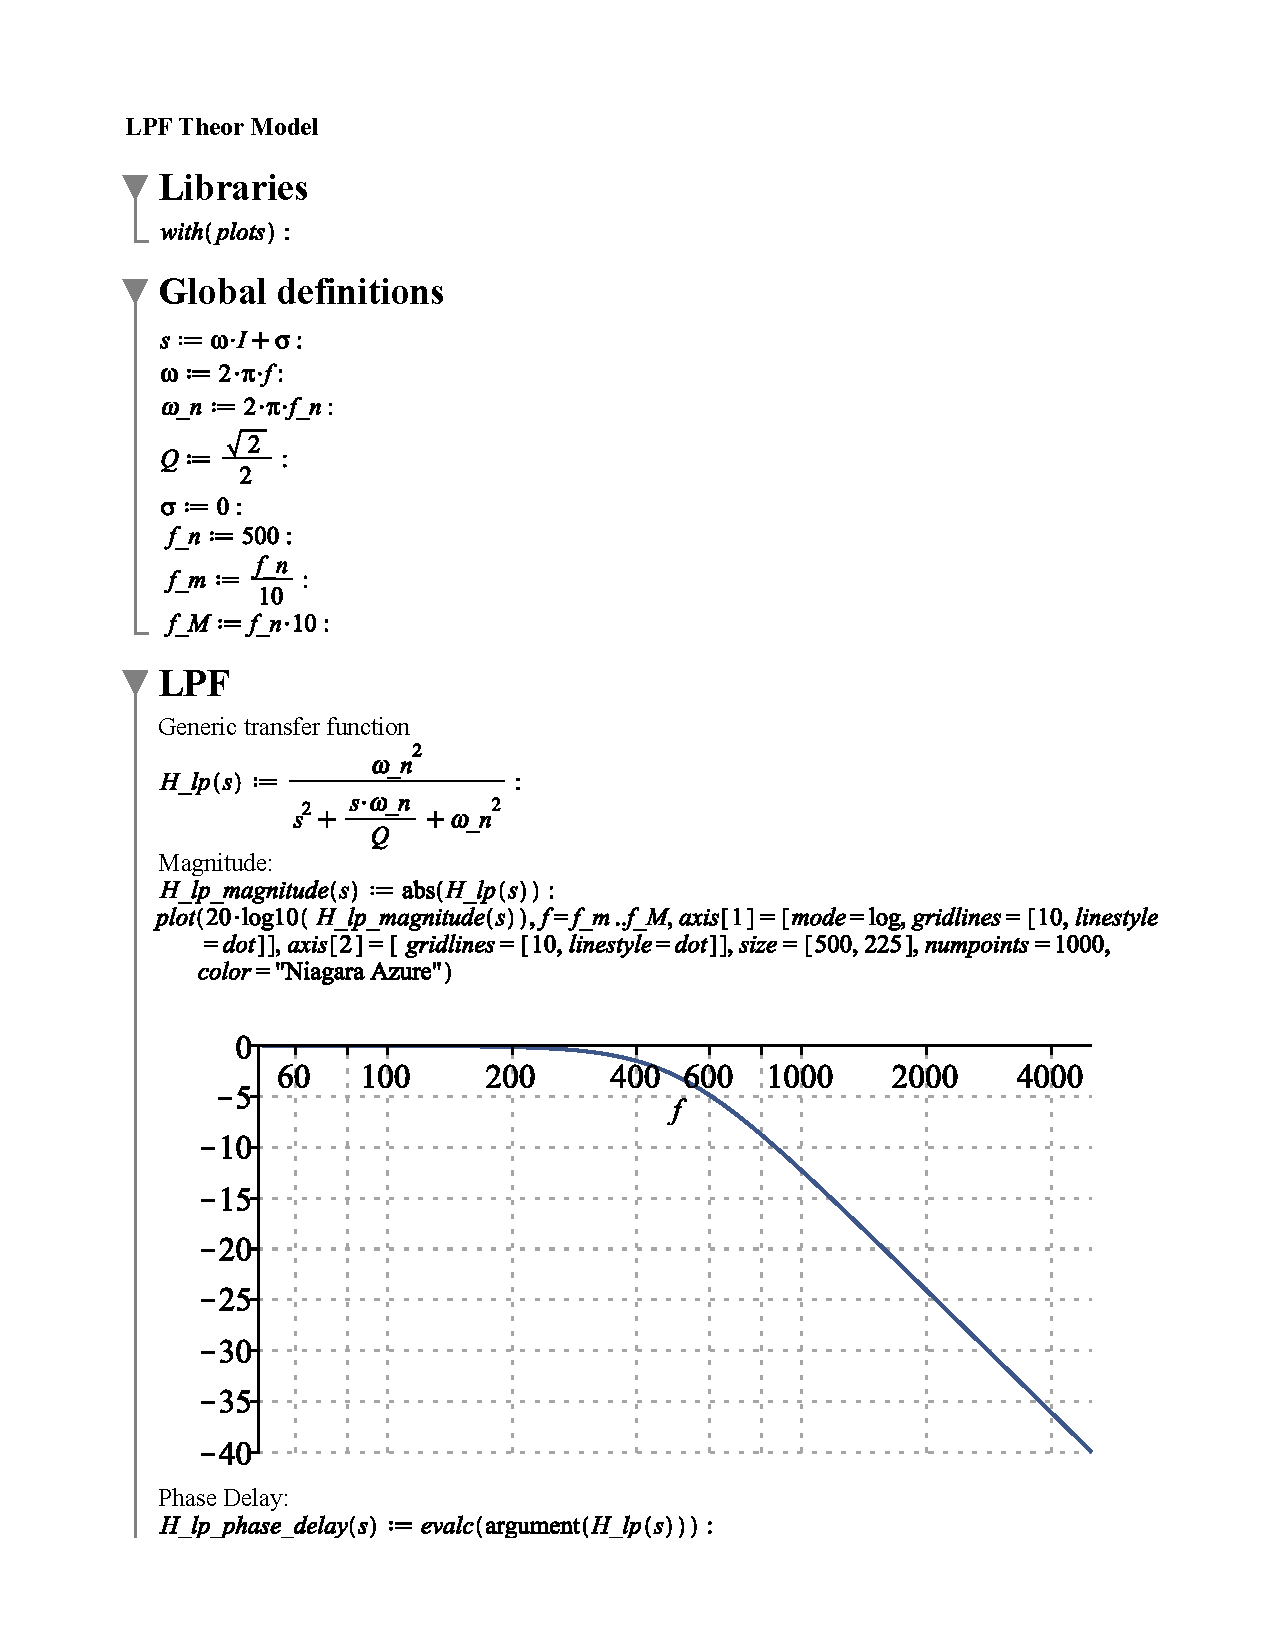
\includepdf[pages=-]{media/maple/lpf_theor-model.pdf}
    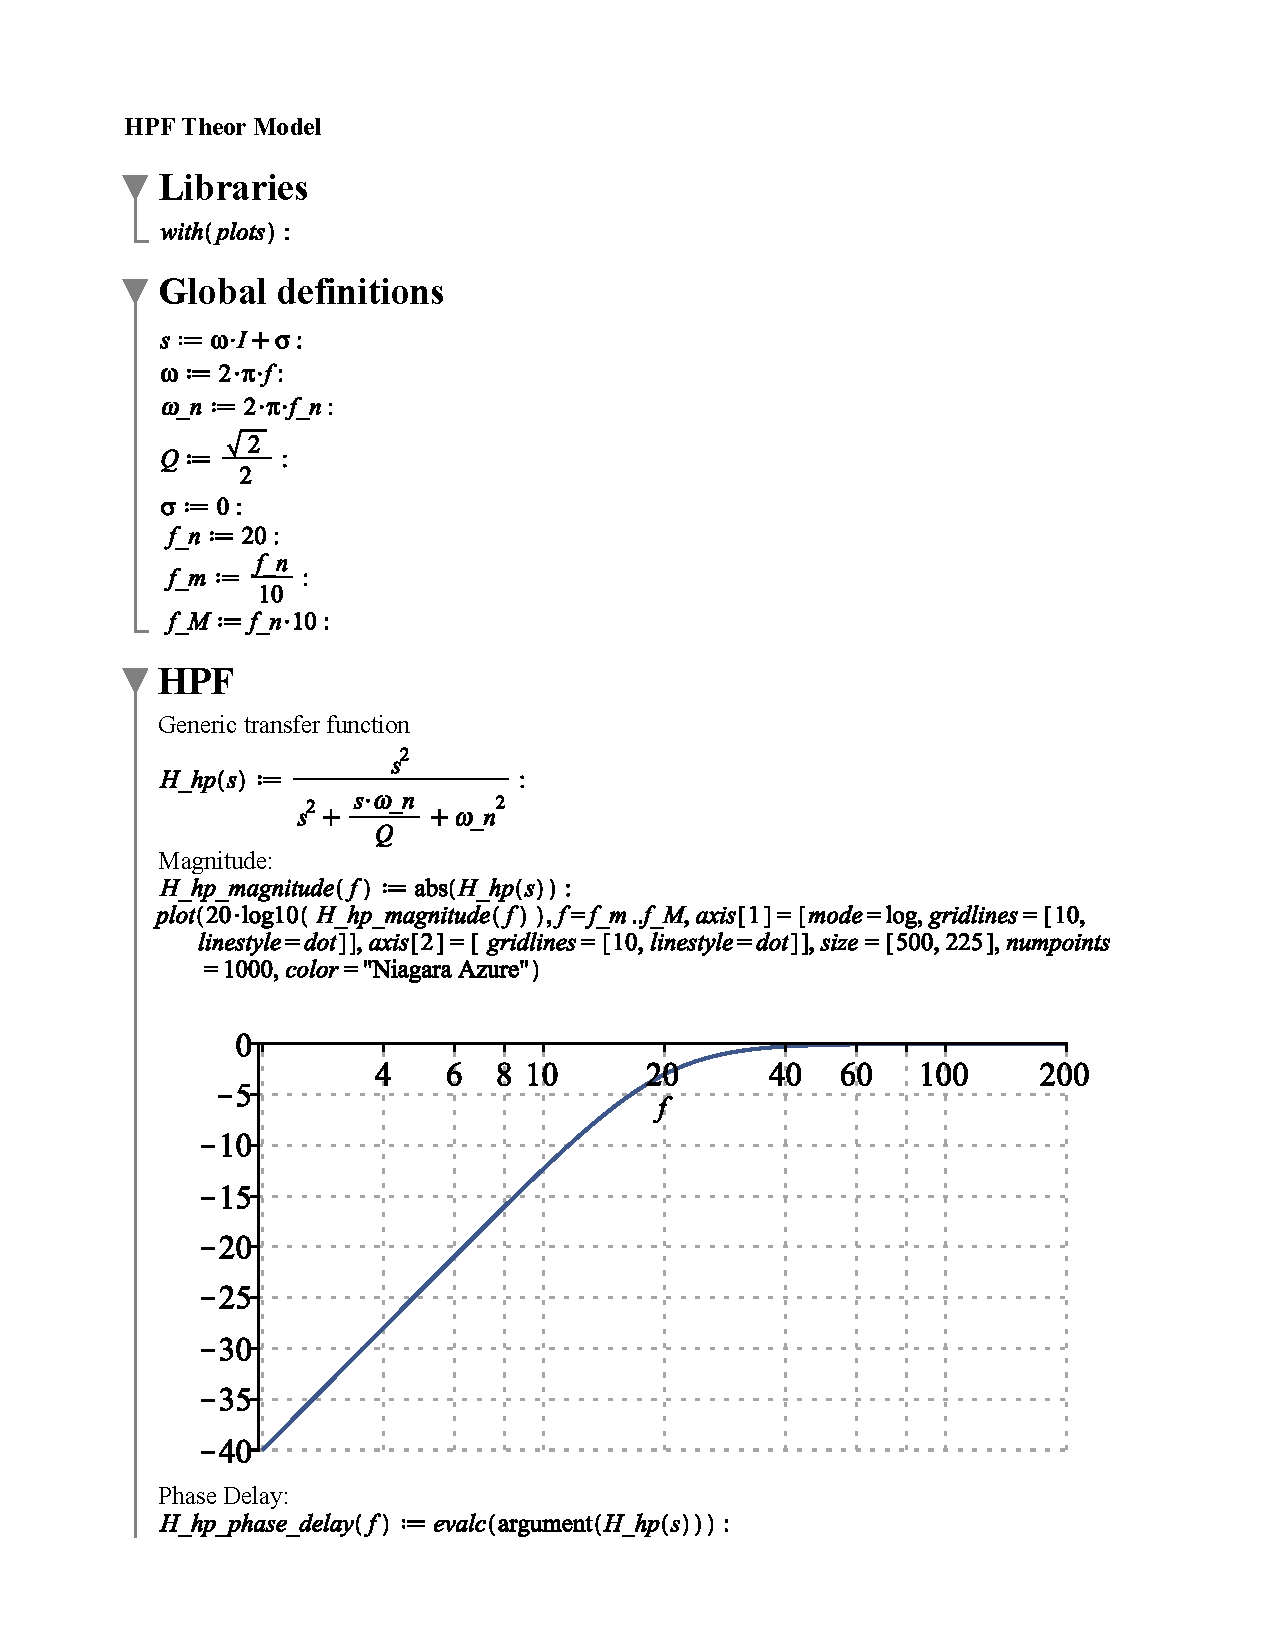
\includepdf[pages=-]{media/maple/hpf_theor-model.pdf}
    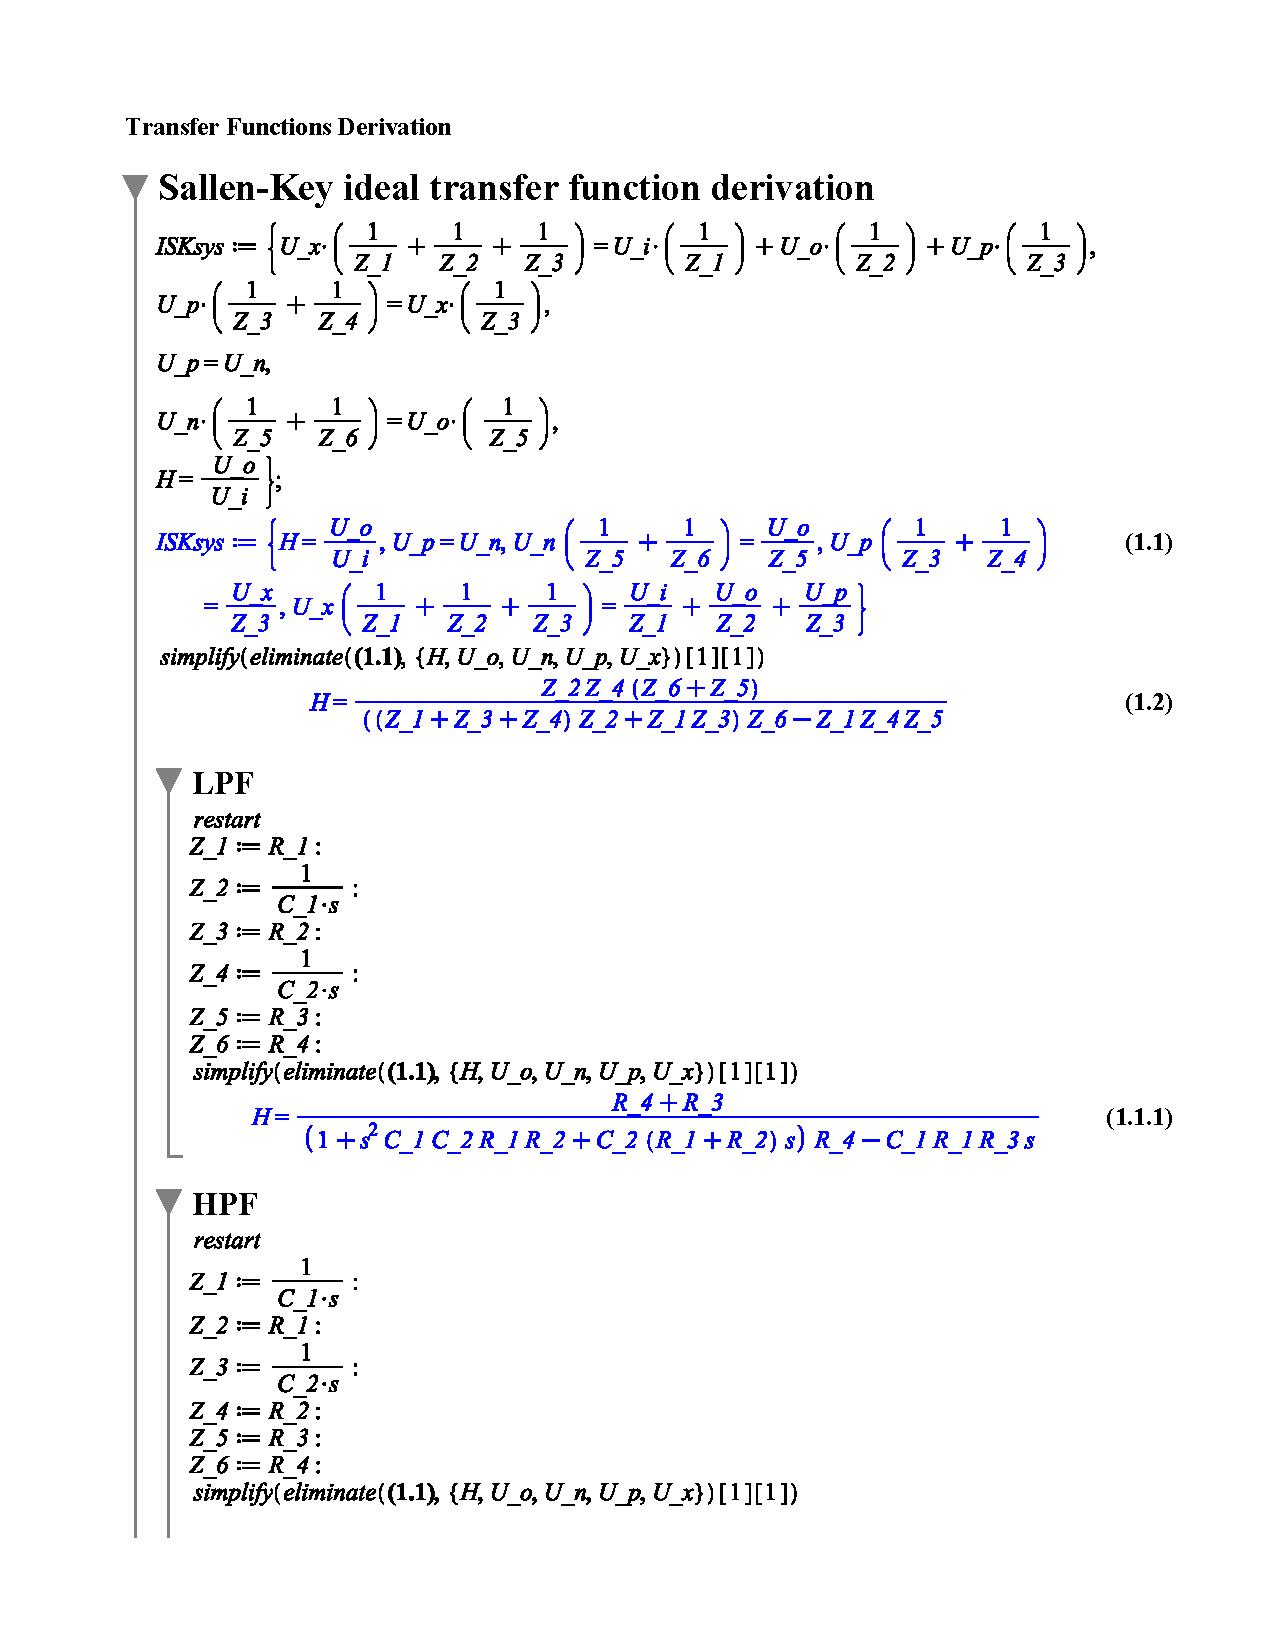
\includepdf[pages=-]{media/maple/tranfer_functions_derivation.pdf}
    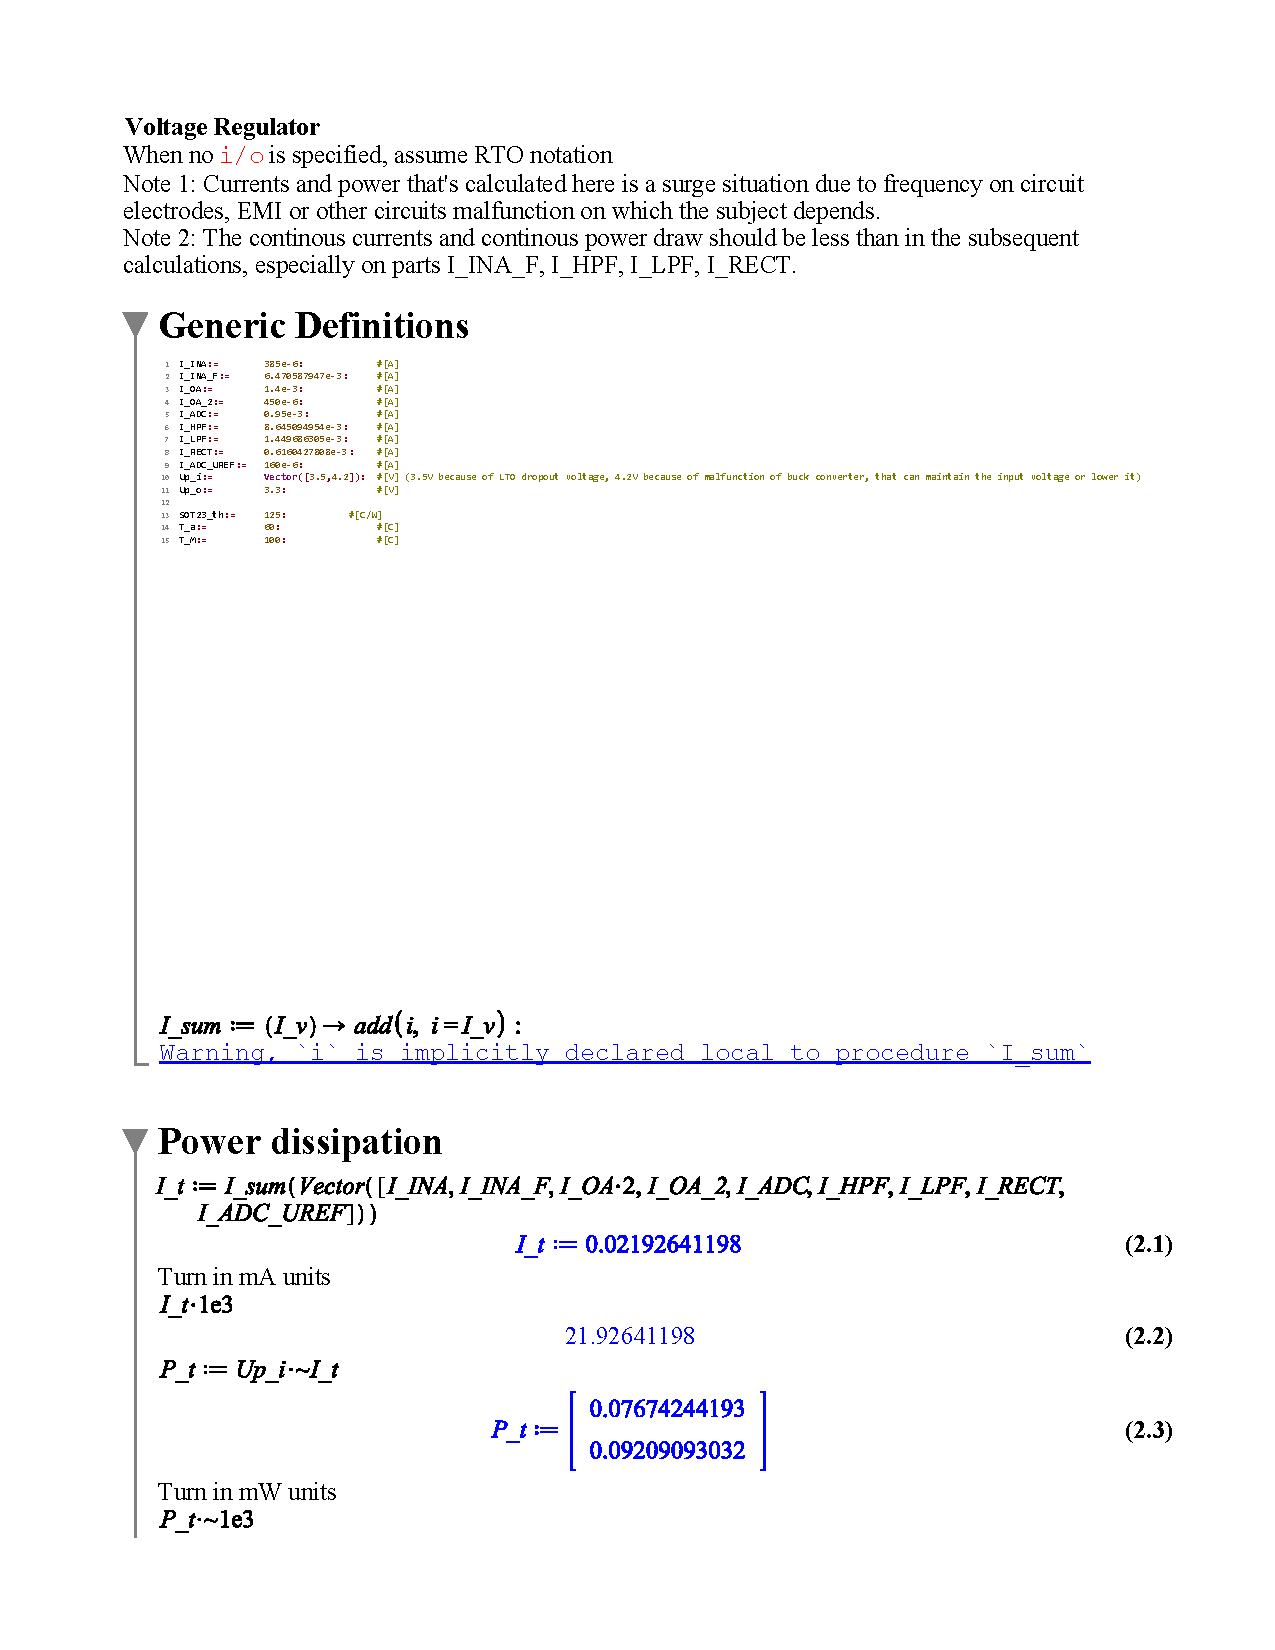
\includepdf[pages=-]{media/maple/voltage_regulator.pdf}
    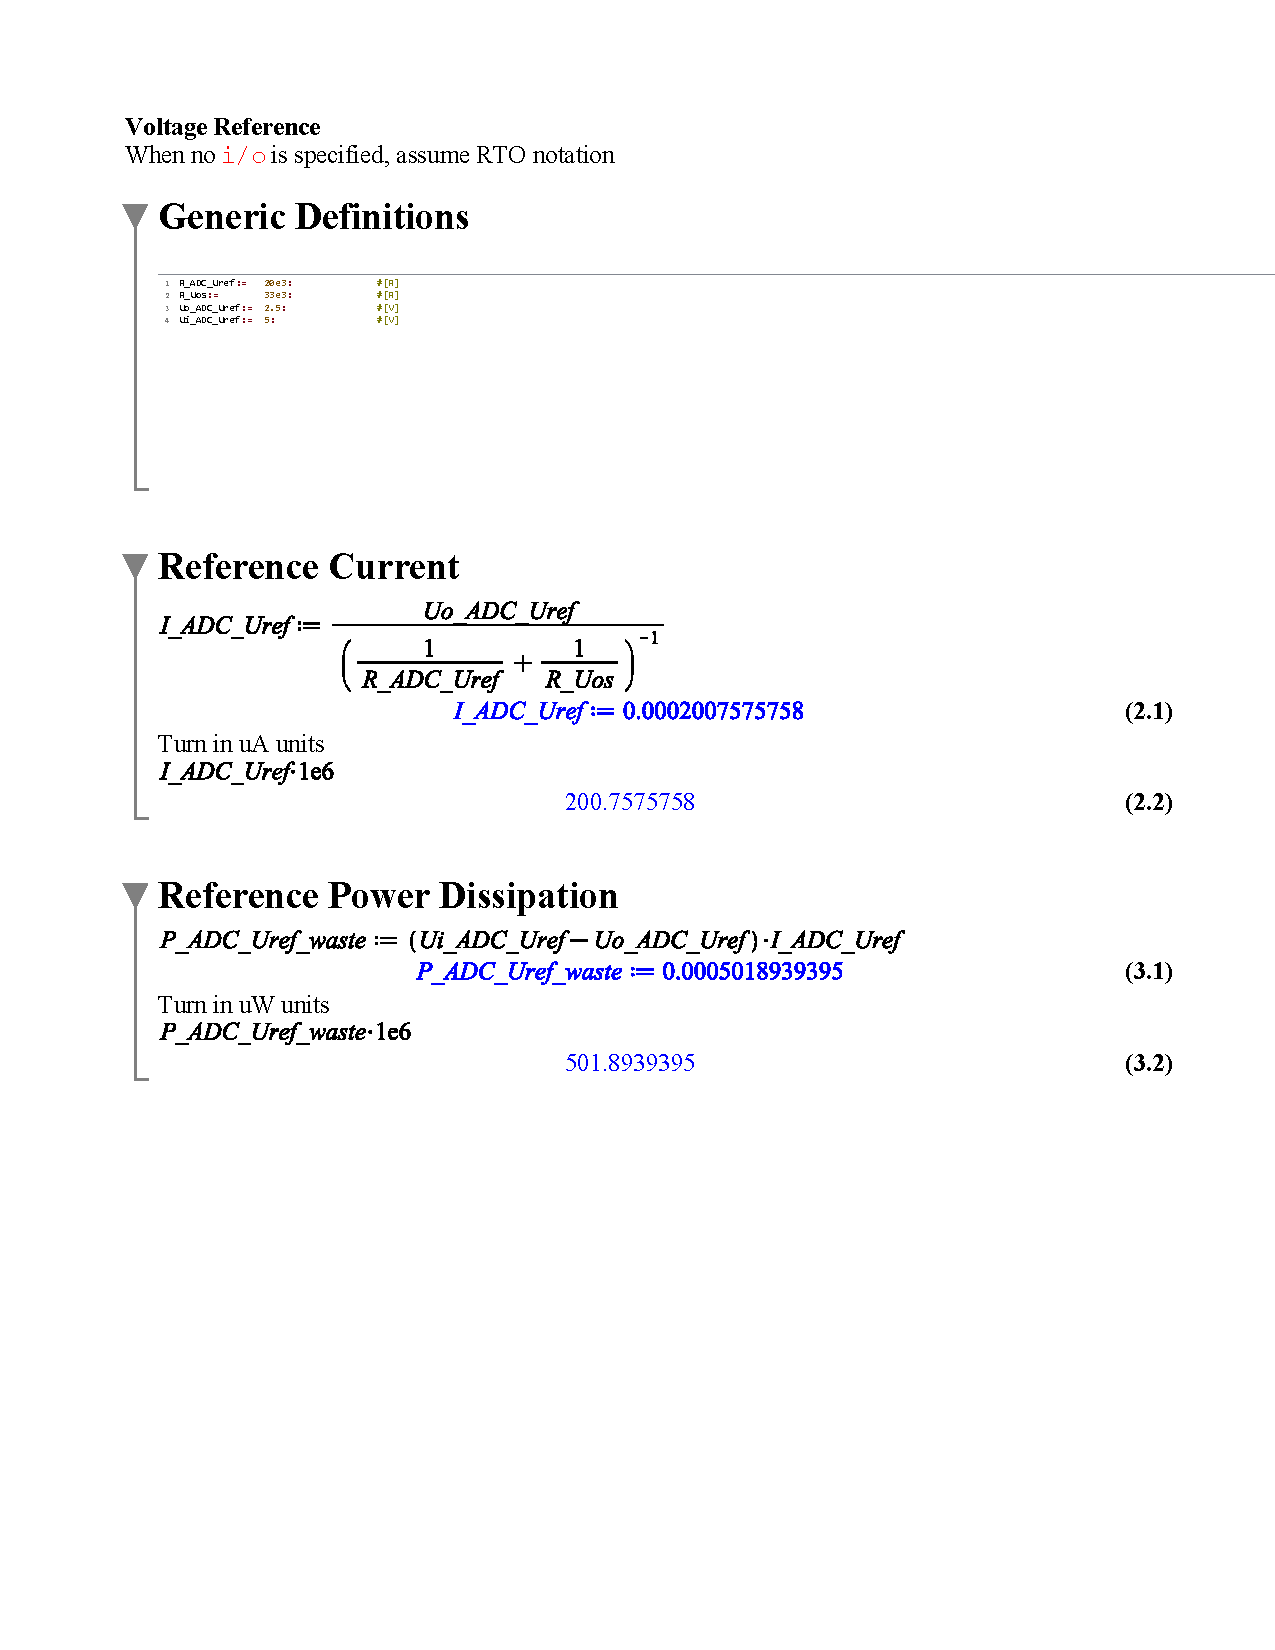
\includepdf[pages=-]{media/maple/voltage_reference.pdf}
    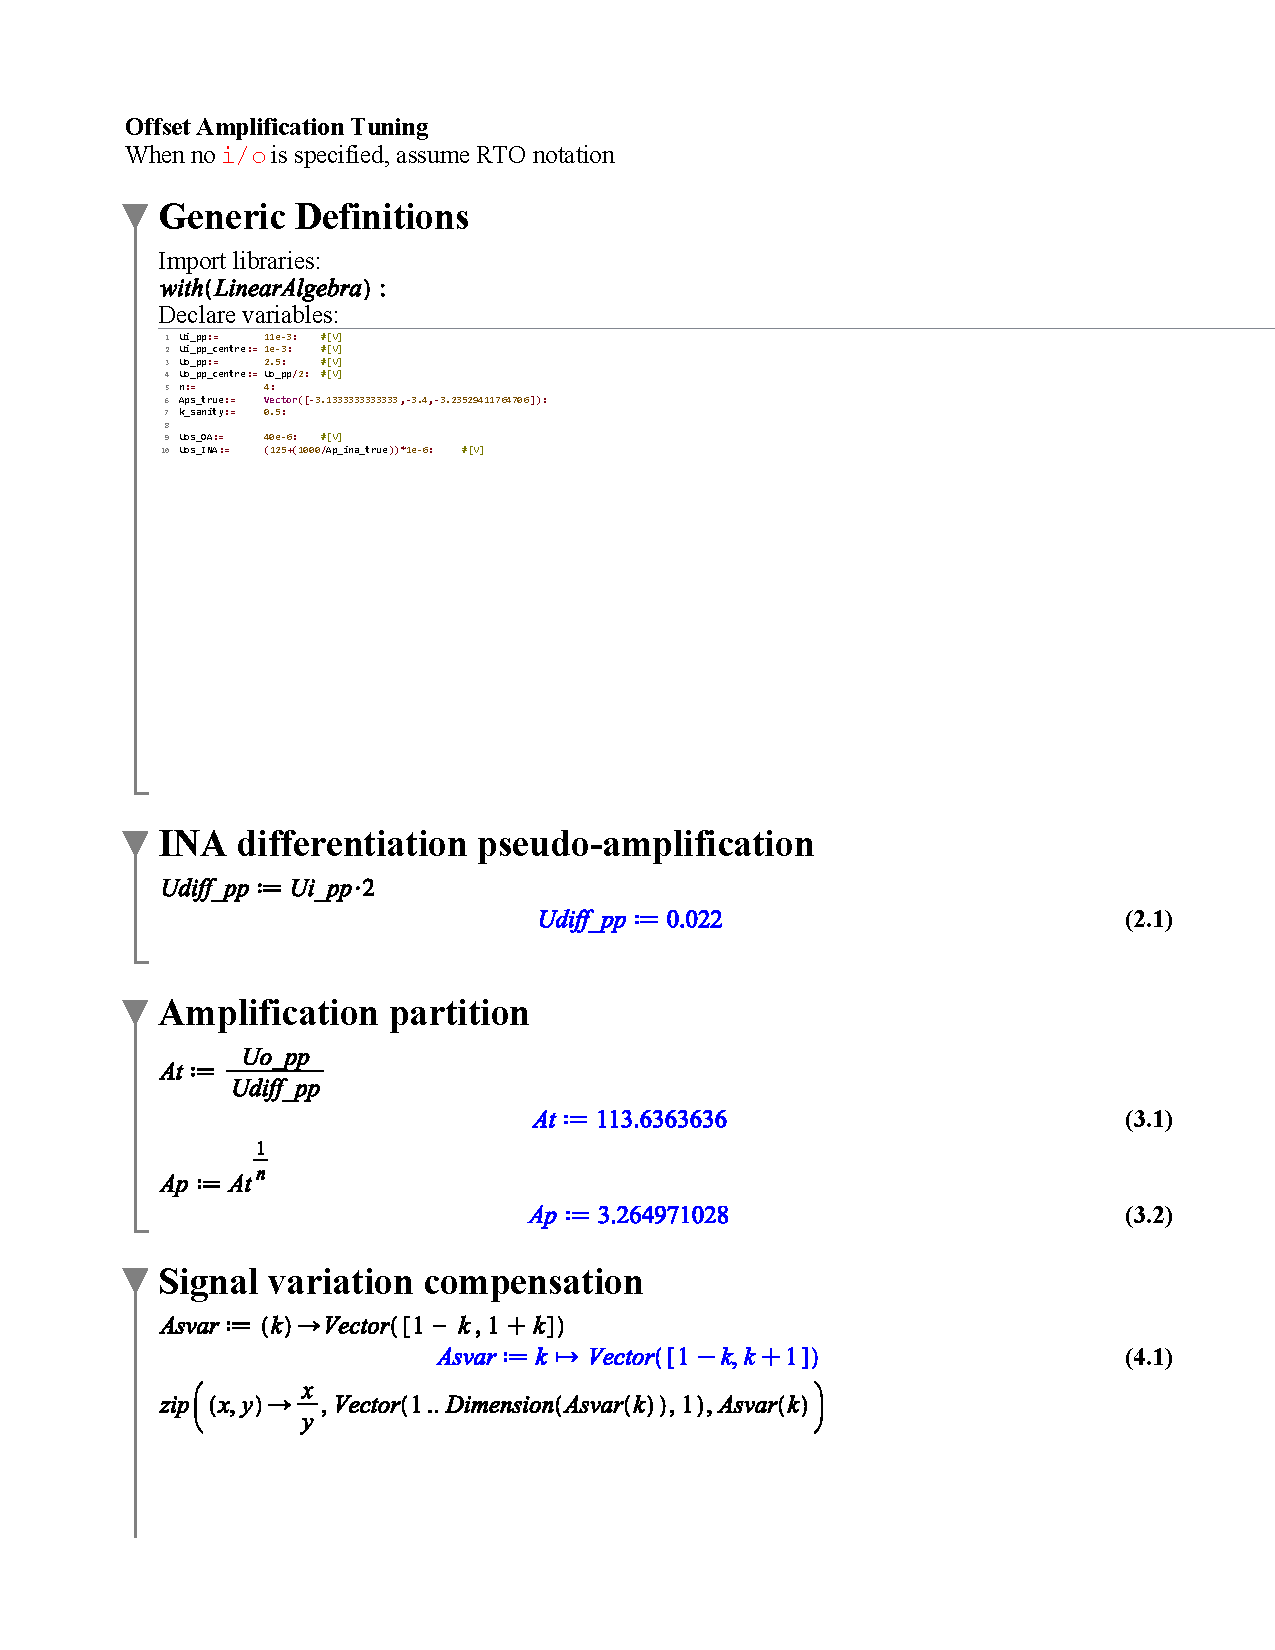
\includepdf[pages=-]{media/maple/offset_amplification_tuning.pdf}
    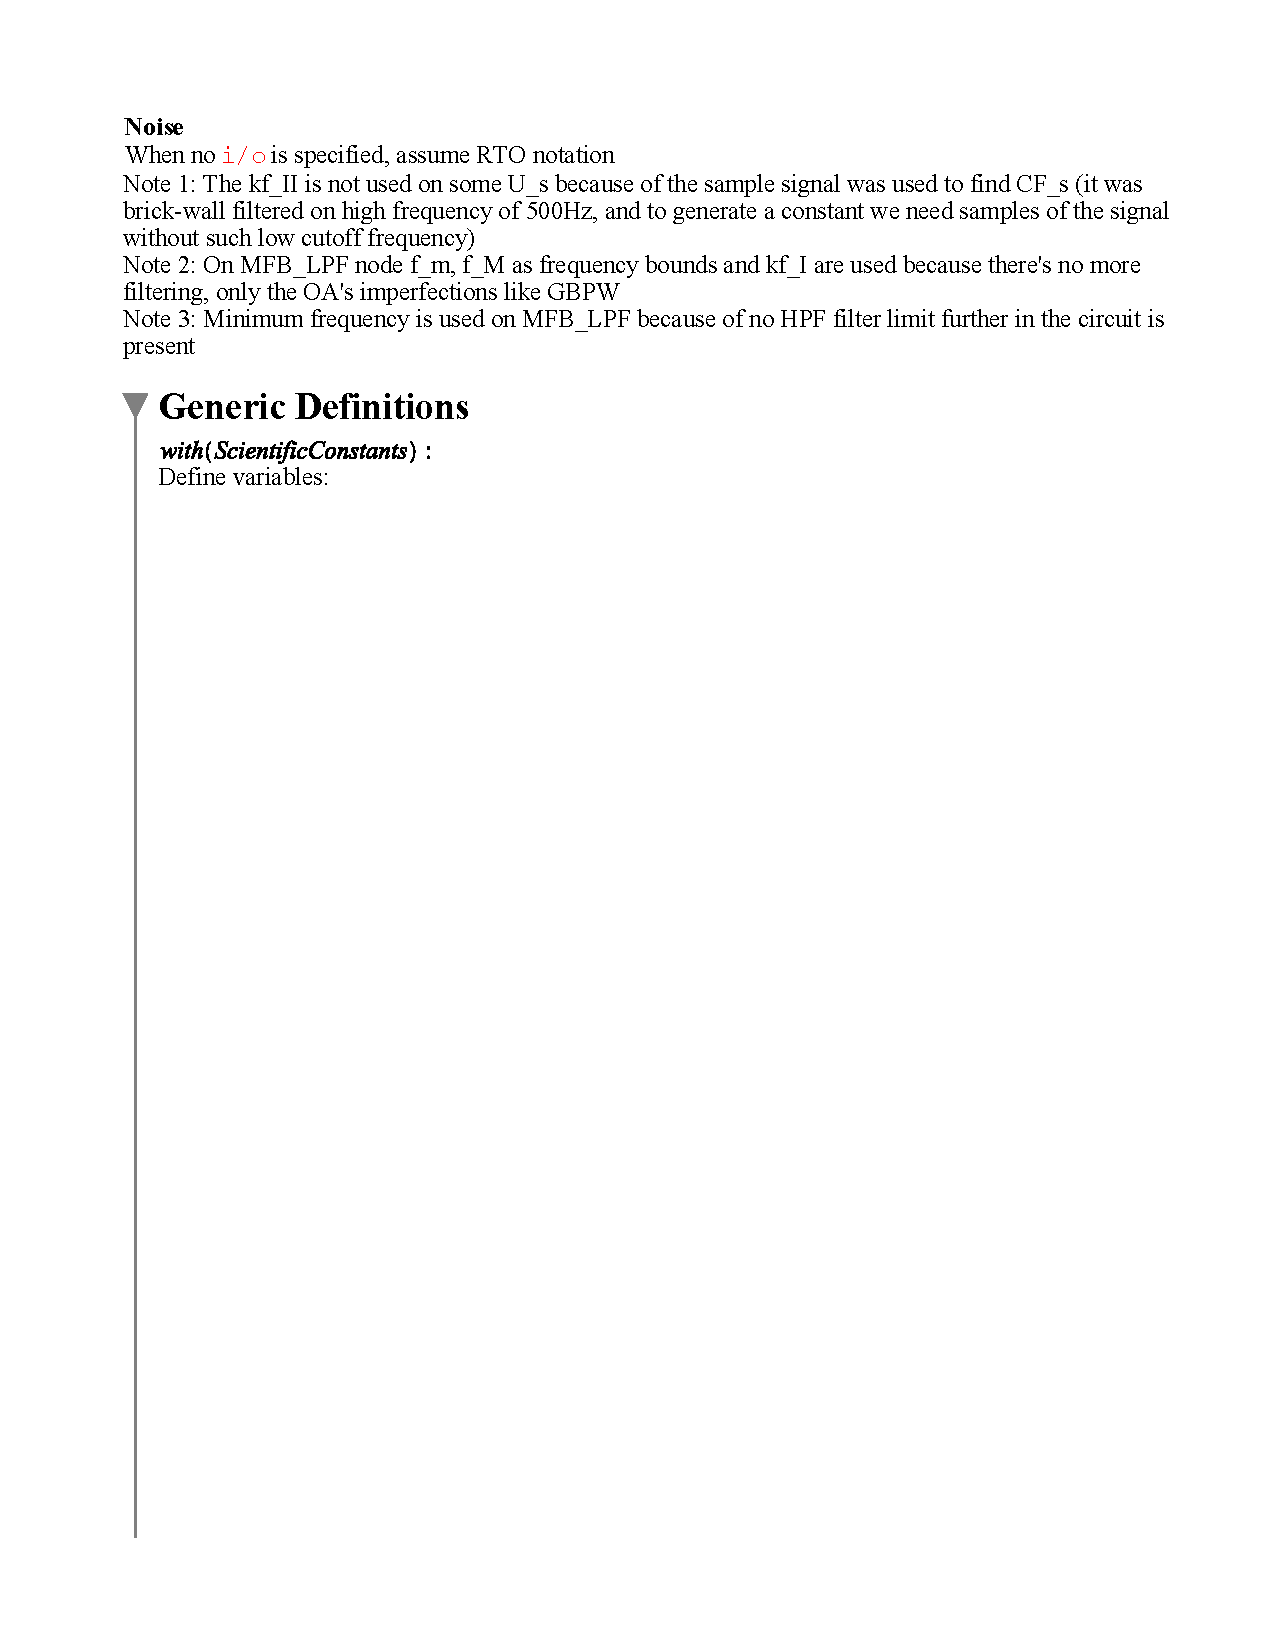
\includepdf[pages=-]{media/maple/noise.pdf}
    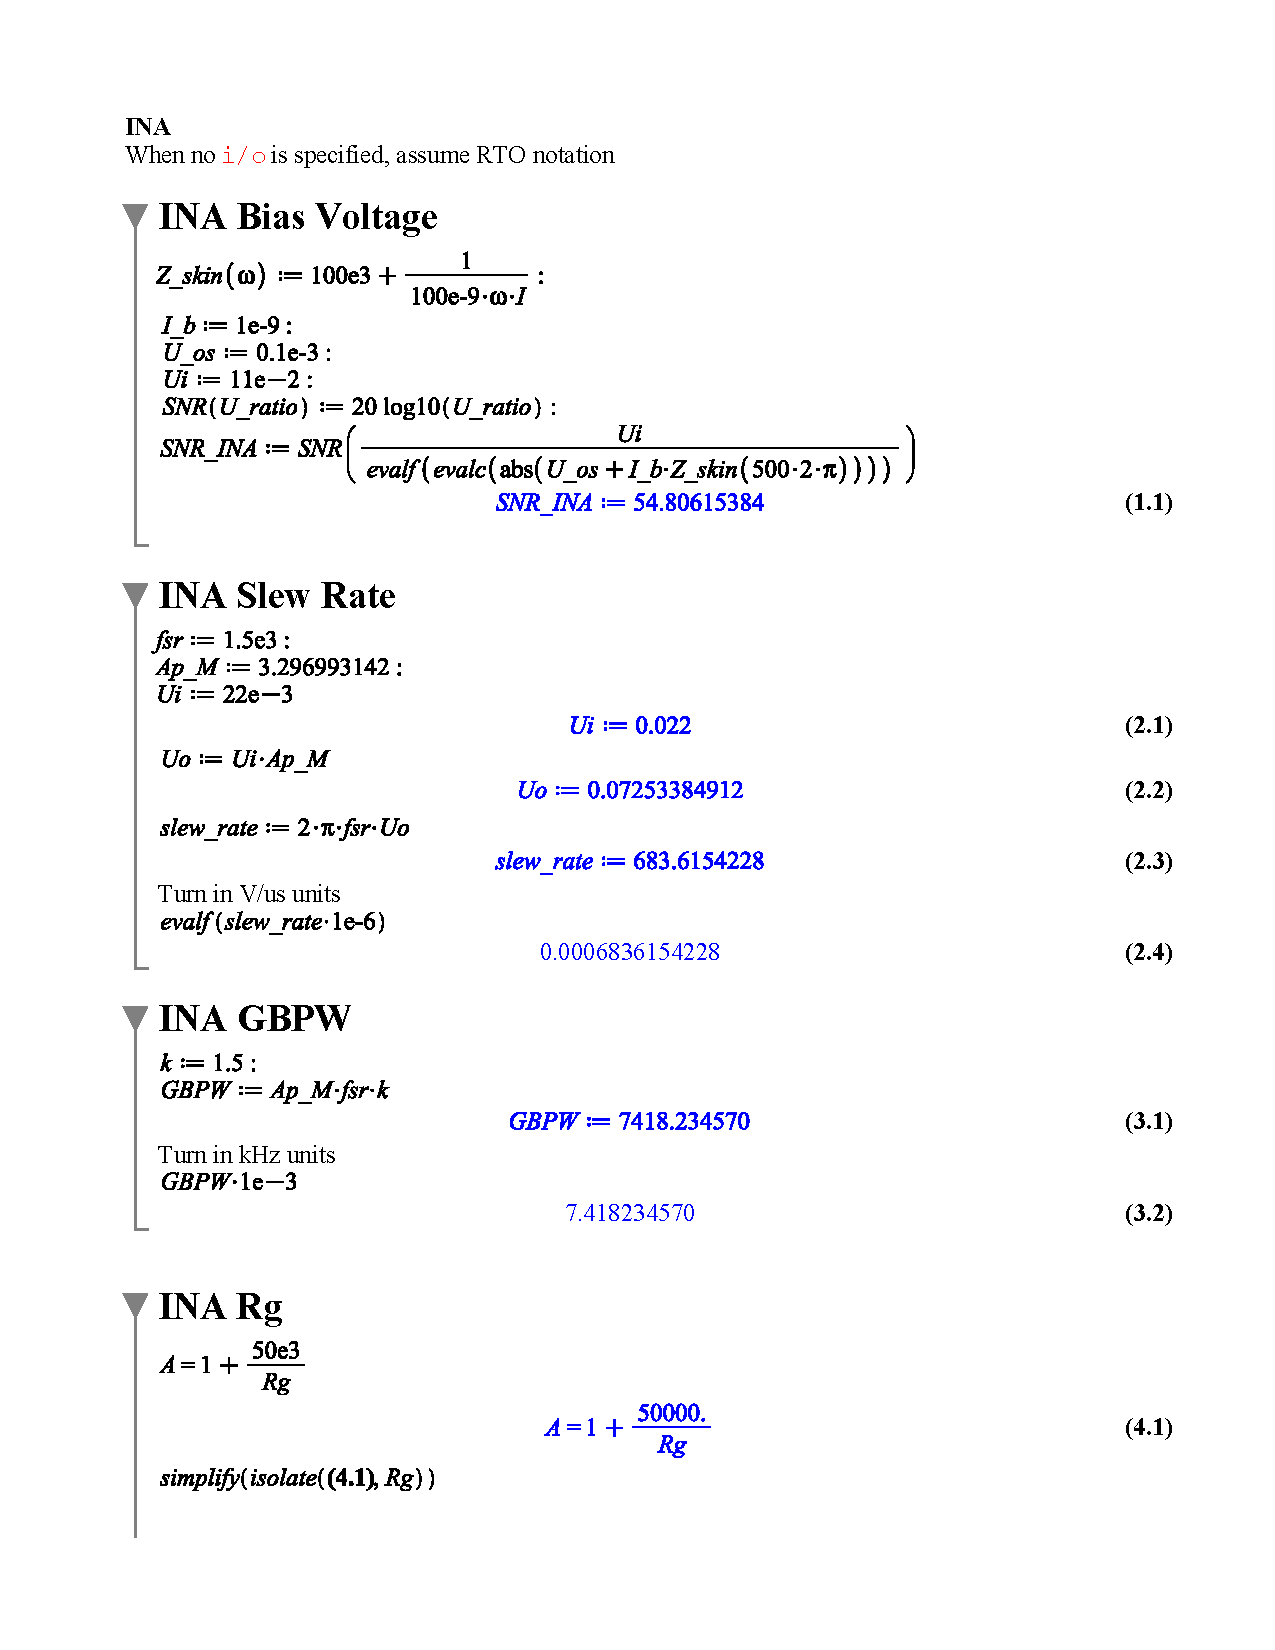
\includepdf[pages=-]{media/maple/INA.pdf}
    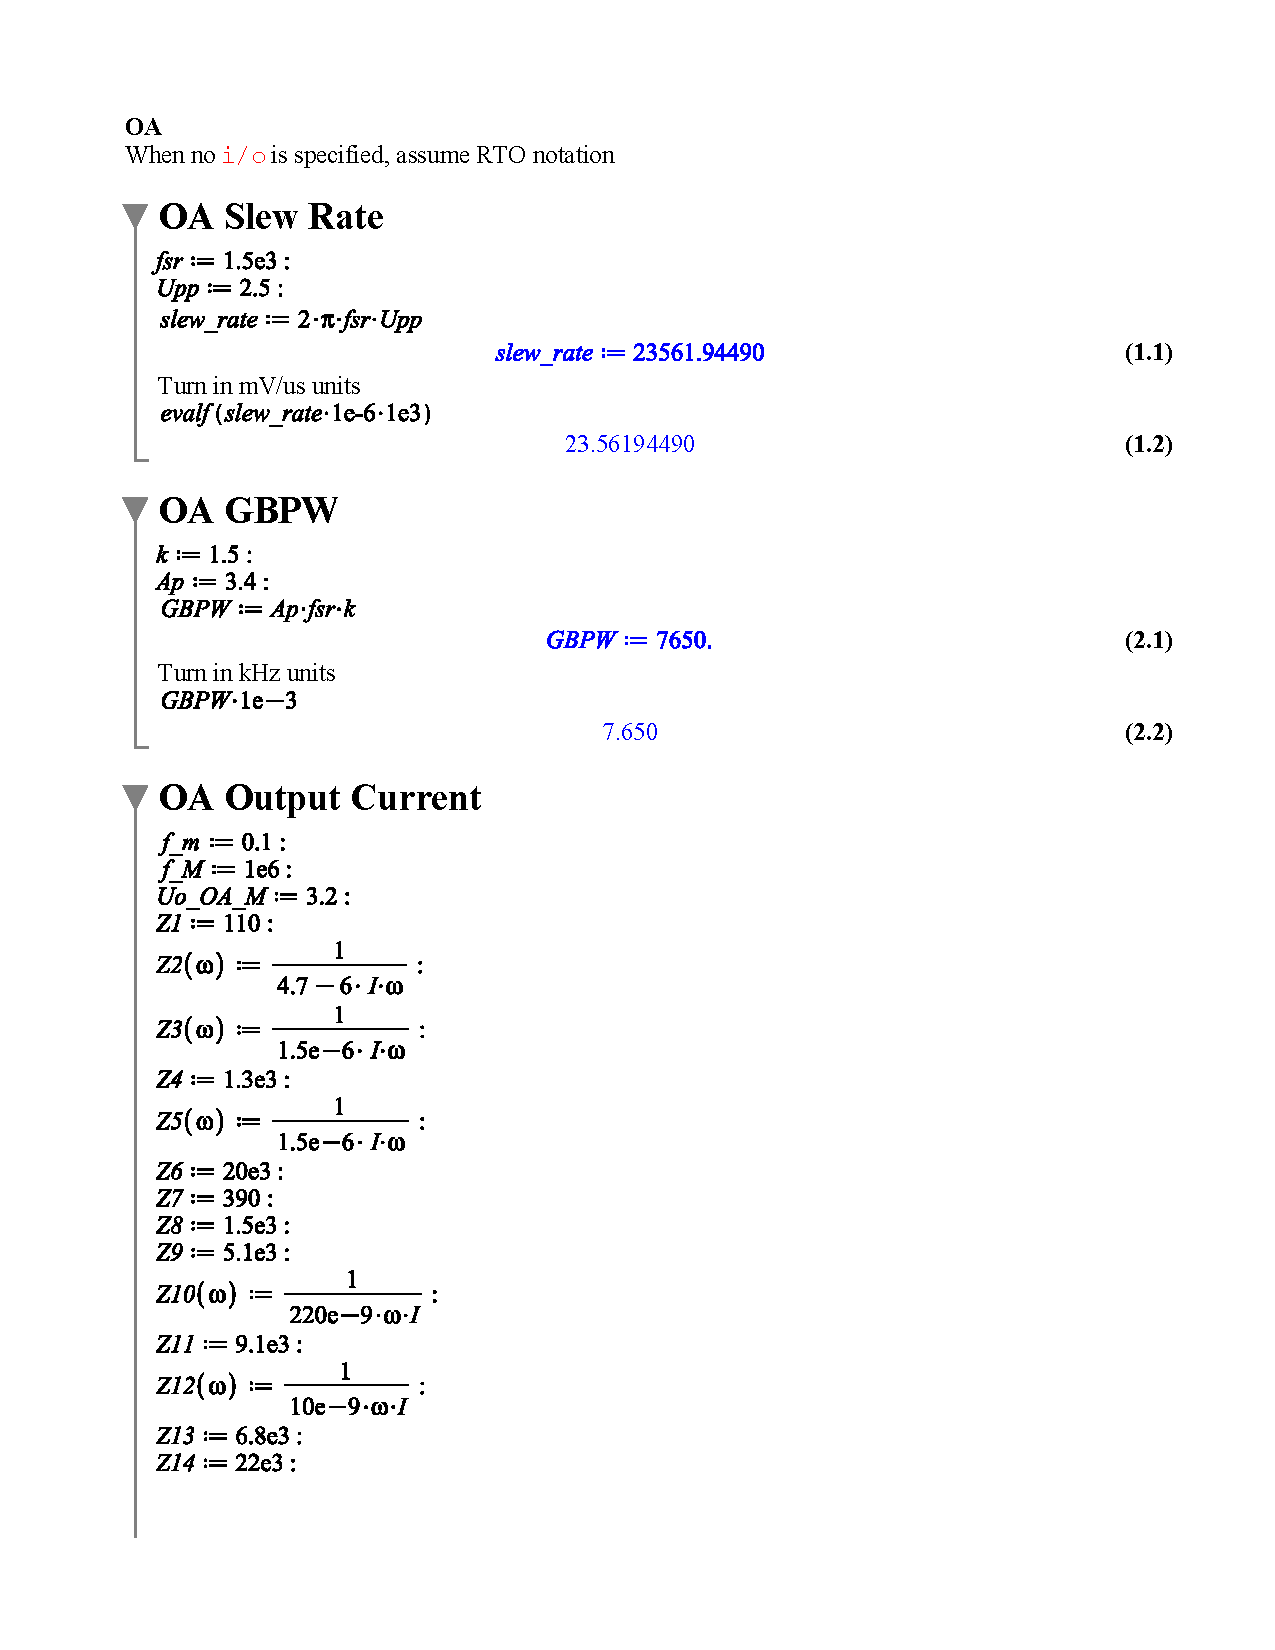
\includepdf[pages=-]{media/maple/OA.pdf}
    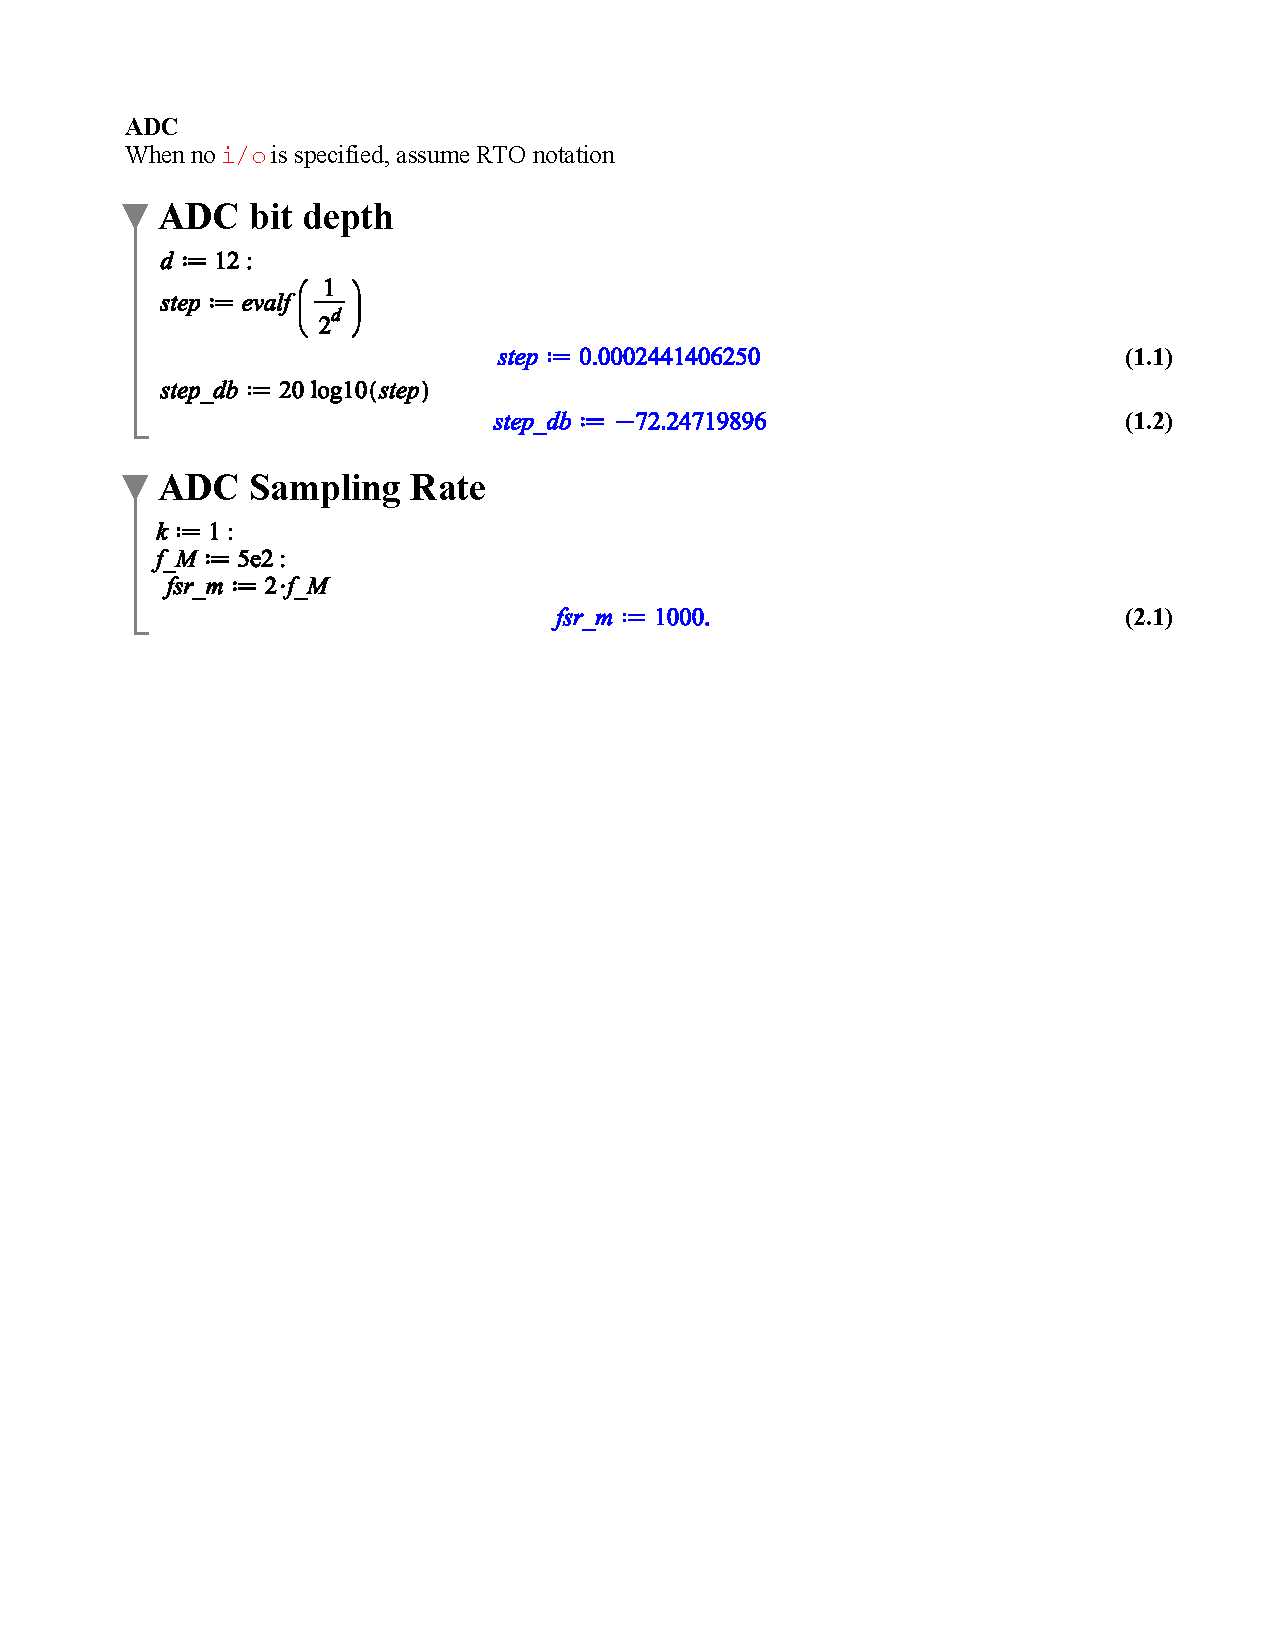
\includepdf[pages=-]{media/maple/ADC.pdf}

    \printbibheading
    \printbibliography[keyword=major, heading=subbibliography, title={Sorgenti Maggiori}]
    \printbibliography[keyword=minor, heading=subbibliography, title={Sorgenti Minori}]
    \printbibliography[keyword=data, heading=subbibliography, title={Sorgenti Dati}]
    \printbibliography[keyword=image, heading=subbibliography, title={Sorgenti Immagini}]
    \printbibliography[keyword=datasheet, heading=subbibliography, title={Sorgenti Datasheet}]
    \printbibliography[keyword=software, heading=subbibliography, title={Sorgenti Software}]
    \printbibliography[keyword=web, heading=subbibliography, title={Sorgenti Componenti}]
\end{document}
